\documentclass{book}

\title{Appunti di Telecomunicazioni}
\author{Stefano Rossini}

\usepackage{bookmark}

\usepackage[italian]{babel}
\usepackage{geometry}
\geometry{a4paper, margin={2.54cm,1.9cm}}

\usepackage{hyperref}
\usepackage{tcolorbox} %for COLORED BOXES 

\usepackage{amsmath}
\usepackage{graphicx}
\graphicspath{{./immagini/}}

\usepackage{url}

\usepackage{physics}

\usepackage{amsfonts} 

\usepackage{gensymb}

\usepackage{textcomp}

\usepackage{tikz}

\usepackage{pgfplots}

\usepackage{amssymb}

\usepackage{imakeidx} 
\makeindex[columns=3, title=Alphabetical Index, intoc]

\hypersetup{
    colorlinks=true,
    linkcolor=blue,
    bookmarksnumbered=true,  % <-- numerazione nelle sezioni del PDF
    pdftitle={Appunti Telecomunicazioni},
    pdfauthor={Autore},
    pdfstartview=FitH
}

\setcounter{secnumdepth}{5}
\setcounter{tocdepth}{4}

\begin{document}

\maketitle

%\setcounter{chapter}{-1}
\section*{Introduzione}

 

Appunti ordinati, con approfondimenti passo-passo, del corso di Telecomunicazioni per il corso di laurea in Ingegneria Elettronica 
presso l’Università Politecnica delle Marche per l'A.A. 2024/2025. \newline
        
Per quelli che seguono il nuovo corso di Ingegneria elettronica: \\
\url{https://www.univpm.it/Entra/Offerta_formativa_1/Corso_di_laurea_triennale_in_Ingegneria_Elettronica_e_delle_Tecnologie_Digitali} \\
cioè la Laurea in Ingegneria Elettronica e delle Tecnologie Digitali, 
il corso prende il nome di Telecomunicazioni digitali. \newline 


Le fonti degli appunti sono le seguenti: 

\begin{itemize}
    
    \item Slide del corso del prof Franco Chiaraluce 
    "Telecomunicazioni digitali A.A. 2024/2025" 
    
    \item Appunti personali e quelli di Damiano Gollinucci presi a lezione
    
    \item Communication Systems Engineering, Second Edition, Proakis - Salehi ISBN 0130617938

\end{itemize}

Chiaraluce è un professore con la P maiuscola: è coinvolgente, esaustivo e chiaro. \newline 

Come dice a lezione, nel corso ci saranno delle salite e poi delle discese, un po' come la vita. \newline 

Venite a lezione, se potete, e chiedete almeno un ricevimento al prof: in tempo massimo una settimana avrete modo di chiedergli qualsiasi dubbio avete in mente. \newline 

Venite a lezione anche per le esercitazioni di Matlab, perchè si potranno capire alcuni argomenti, specialmente quelli finali: dal metodo "carta e penna" al metodo iterativo e di programmazione. \newline 

Sfruttate il ricevimento il più possibile, perchè, giustamente, a lezione non vi verranno tutti i tre-miliardi di dubbi sul corso, 
specialmente quelli in cui il prof lascia le slide senza spiegazioni e solo con la formula. \newline 

La cosa più importante dell'orale è come ci si arriva alla formula. \newline 

È un po' come la vita: l'importante è il viaggio, non dove si arriva. \newline 

È altamente consigliato studiare e superare prima l’esame di teoria dei segnali, o come si chiama adesso "Segnali Determinati e Aleatori", 
perchè non capirete nulla sul corso, ve lo posso assicurare mettendo la mano sul fuoco. \newline 

Ogni concetto scritto in queste dispense, fa riferimento al corso precedente, o come lo chiama il professore a "Telecomunicazioni 1", perchè questa è "Telecomunicazioni 2". \newline 

Se vuoi dare un'occhiata ai miei vecchi appunti del corso di Teoria dei Segnali: \\
\url{https://github.com/ciccio25/appunti-teoria-dei-segnali} \newline 

I concetti importanti degli altri corsi precedenti che non sono quelli di Chiaralce sono importanti ma non fondamentali: ci serviranno i concetti base. \newline 

Lascerò dei link a video e/o spiegazioni esterne per ulteriori approfondimenti. \newline 

Per qualsiasi domanda, se trovi qualche errore grammaticale o hai bisogno di chiarimenti, scrivimi a \href{mailto:rossini.stefano.appunti@gmail.com}{rossini.stefano.appunti@gmail.com} o contattami su Whatsapp se hai il mio numero di cellulare personale. \newline

Se trovi qualche errore e/o vuoi contribuire agli appunti, 
puoi aprire un Issue sulla repository degli appunti di GitHub. \newline 

Buono studio e buona lettura \newline

\newpage 







\tableofcontents

\section*{Tabella lettere greche utili per il corso}

\begin{center}
\begin{tabular}{ c c c }
    
Lettera maiuscola & Lettera minuscola & Nome lettera greca \\
\hline 
A & $\alpha$ & Alfa \\ \\
B & $\beta$ & Beta \\ \\
$\Gamma$ & $\gamma$ & Gamma \\ \\
$\Delta$ & $\delta$ & Delta \\ \\  
E & $\varepsilon$ & Epsilon \\ \\
H & $\eta$ & Eta  \\ \\ 
$\Theta$ & $\theta$ & Theta \\ \\  
K & $\kappa$ & Kappa \\ \\ 
$\Lambda$ & $\lambda$ & Lambda \\ \\ 
M & $\mu$ & Mu \\ \\ 
$\Pi$ & $\pi$ & Pi \\ \\ 
P & $\rho$ & Rho \\ \\
$\Sigma$ & $\sigma$ & Sigma \\ \\  
T & $\tau$ & Tau \\ \\ 
$\Phi$ & $\phi$ & Phi \\ \\
X & $\chi$ & Chi \\ \\ 
$\Psi$ & $\psi$ & Psi \\ \\ 
$\Omega$ & $\omega$ & Omega  




\end{tabular}
\end{center}

\newpage 

\chapter{Rumore nei sistemi lineari}

\begin{figure}[h]
    \centering
    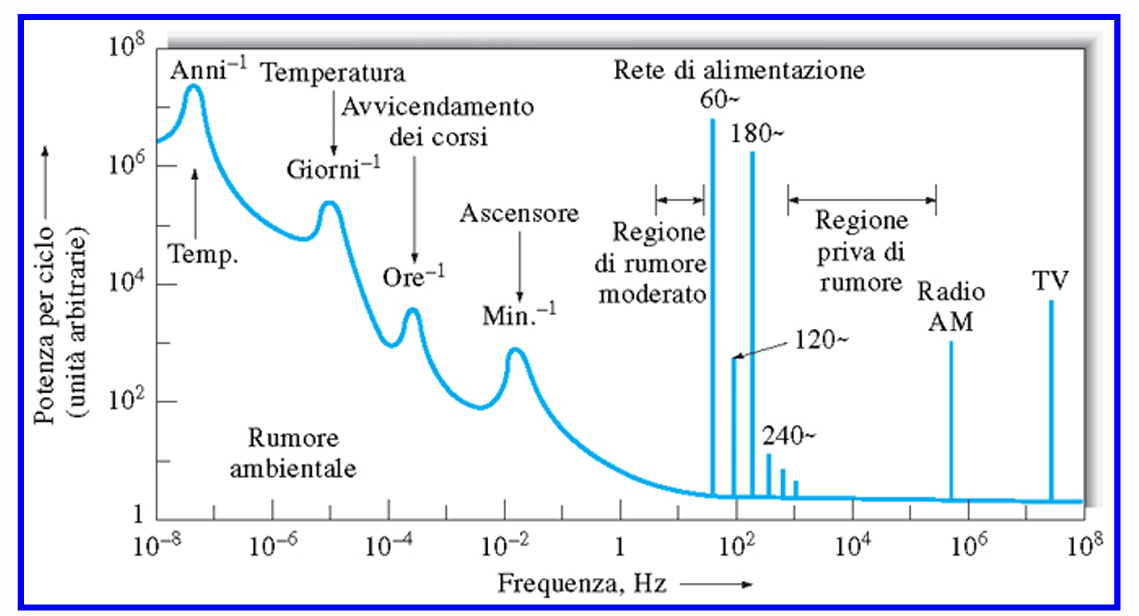
\includegraphics[scale = 0.8]{Rumore in base alla frequenza.PNG}
\end{figure}

\newpage 

\section{Banda equivalente di rumore}
\footnote{Slide del prof | Parametri di rumore sistema lineare | pag 1 \\  
Appunti di Damiano| pag 1} 

Dato un sistema lineare: 

\begin{figure}[h]
    \centering
    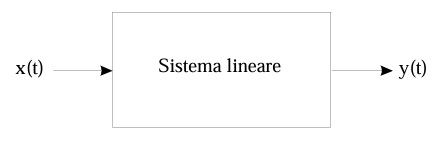
\includegraphics[scale = 1]{Blocco sistema lineare.PNG}
\end{figure}

dove x(t) è il segnale di ingresso e y(t) è il segnale di uscita dal sistema lineare, 
dal corso di Teoria dei Segnali, è noto che una generica rete 2-porte, anche contenente elementi attivi, 
è responsabile dell'introduzione di un contributo di rumore termico, 
che si sovrappone al segnale utile (i.e. segnale di ingresso) e ne degrada le caratteristiche. \newline 

\begin{tcolorbox}
    Un breve ripasso da Tds: \\
    \url{https://github.com/ciccio25/appunti-teoria-dei-segnali/blob/main/Appunti%20Teoria%20dei%20segnali.pdf} \\
    Capitolo 5 - Sistemi lineari - pag 41
\end{tcolorbox}

Allo stesso tempo, un rumore termico presente all'ingresso di una rete lineare, 
viene modificato dal transito di essa, e si ritrova in uscita amplificato (o attenuato) 
oltre che, eventualmente, con una minore occupazione spettrale (determinata dalle caratteristiche filtranti della rete resistiva). \newline 

\begin{tcolorbox}
    Un sistema lineare, a differenza di un sistema non lineare, può solo togliere le componenti in frequenza dal segnale di ingresso iniziale e non ne aggiunge di nuove
\end{tcolorbox}

Questi aspetti devono essere combinati per poter analizzare come la potenza di rumore viene alternata dal passaggio attraverso un sistema lineare 
e, soprattutto, come tale potenza aumenta quando più sistemi lineari vengono posti in cascata. \newline 

Un primo concetto utile, nel contesto delineato, è quello di banda equivalente di rumore. \newline 

Una rete 2-porte lineare è caratterizzata dalla sua funzione di trasferimento H(f) . \newline 

Quando un rumore termico, con densità spettrale di potenza bilatera $\frac{\eta}{2}$ (costante sia per le frequenze positive che per quelle negative) è applicato all'ingresso della H(f), 
la potenza di rumore in uscita sarà data da: 

{
    \Large 
    \begin{equation}
        \begin{split}
            <n^{2}>
            &= 
            \int_{-\infty}^{+\infty}
            p_{n_h}(f) 
            df
            \\
            &= 
            \int_{-\infty}^{+\infty}
            p_h(f) \cdot p_n(f) 
            df
            \\
            &= 
            \int_{-\infty}^{+\infty}
            \abs{H(f)}^{2} \cdot \abs{N(f)}^{2}
            df
            \\
            &= 
            \int_{-\infty}^{+\infty}
            \abs{H(f)}^{2} \cdot \frac{\eta}{2}
            df
            \\
            &=
            \frac{\eta}{2}
             \int_{-\infty}^{+\infty}
            \abs{H(f)}^{2} 
            df
        \end{split}
    \end{equation}
}

dove: 

\begin{itemize}
    \item $p_{n_h}(f)$ si intende la potenza del rumore (noise dall'inglese) dopo il sistema lineare 
    \item $p_h (f)$ si intende la potenza del sistema lineare 
    \item $p_n (f)$ si intende la potenza del rumore 
\end{itemize}  

\newpage 

\begin{tcolorbox}
    Per ripassare i sistemi lineari \newline 

    Da \url{https://github.com/ciccio25/appunti-teoria-dei-segnali/blob/main/Appunti%20Teoria%20dei%20segnali.pdf} \\
    Capitolo 5.2 Densità spettrale di energia e di potenza di un filtro | pag 44 \newline 

Dato x(t) il segnale di ingresso e y(t) il segnale di uscita di un sistema lineare, 
possiamo definire le loro rappresentazioni in Fourier come $X(\omega)$ e $Y(\omega)$. \newline 

Essendo: 

{
    \Large 
    \begin{equation}
        Y(\omega) = H(\omega) X(\omega)
    \end{equation}
}

le densità spettrali di energia (ove applicabili) dei segnali in ingresso e in uscita sono tra 
loro legate dalla seguente relazione: 

{
    \Large 
    \begin{equation}
        \abs{Y(\omega)} ^{2} 
        = 
        \abs{H(\omega) X(\omega)} ^{2} 
        = 
        \abs{H(\omega)} ^{2} \cdot \abs{X(\omega)} ^{2}
    \end{equation}
}

Una relazione analoga vale per gli spettri di potenza, indicati con $p_x (\omega)$ 
(per l'ingresso) e $p_y (\omega)$ (per l'uscita): 

{
    \Large 
    \begin{equation}
        p_y (\omega) = \abs{H(\omega)} ^{2} p_x (\omega)
    \end{equation}
}

$\blacksquare$ \newline 

Dunque, la densità in uscita si ottiene moltiplicando la densità in ingresso 
per il modulo al quadrato della funzione di trasferimento. \newline 


    Per ripassare il rumore \newline 

    Da \url{https://github.com/ciccio25/appunti-teoria-dei-segnali/blob/main/Appunti%20Teoria%20dei%20segnali.pdf} \\
    Capitolo 14.1 Un esempio di processo stocastico: il rumore termico | pag 162 - 163 \newline 

    Ponendo T come il valore della temperatura assoluta a cui si trova il sistema lineare in kelvin, 
    dove la relazione tra temperatura espressa in kelvin e gradi celsius è la seguente: 

    {
        \Large 
        \begin{equation}
            0\text{ }K = -273.15 \text{ } ^{\circ} C
        \end{equation}
    }


    Sapendo che: 

{
    \Large 
    \begin{equation}
        K = 1.38 \cdot 10^{-23} \frac{J}{^{\circ} K}
    \end{equation}
}

è la costante di Boltzmann. \newline 

Sapendo che il rumore è un processo "stocastico", possiamo esprimere la potenza del rumore indipendente dal tempo come: 

{
    \Large 
    
        \begin{equation}
                <P_n>
                = 
                KTB
        \end{equation}
    
}

dove $P_n$ è la "potenza disponibile". \newline 

La densità spettrale di potenza sarà: 

{
    \Large 
    \begin{equation}
        \begin{split}
        p_n(f) 
        &= 
        \frac{KT}{2}
        \\
        &= \frac{\eta}{2}
        \end{split}
    \end{equation}
}

\end{tcolorbox}

L'espressione: 

{
    \Large 
    \begin{equation}
        <n^{2}>
        =
            \frac{\eta}{2}
             \int_{-\infty}^{+\infty}
            \abs{H(f)}^{2} 
            df
    \end{equation}
}

mette in evidenza che, una volta assegnato il valore di $\frac{\eta}{2}$, 
la potenza di rumore in uscita dipende solo dall'andamento della funzione di trasferimento del sistema lineare. \newline 

Sapendo che: 

{
    \Large 
    \begin{equation}
        \frac{1}{2} \int_{-\infty}^{+\infty} \abs{H(f)}^{2} df = \abs{H_0}^{2} B_N
    \end{equation}
}

dove: 

\begin{itemize}
    \item $\abs{H_0}$ è l'ampiezza del sistema lineare 
    \item $B_N$ è la banda del rumore di ingresso al sistema lineare
\end{itemize}

Isolando $B_N$ dalla formula precedente, con dei semplici passaggi algebrici: 

{
    \Large 
    \begin{equation}
        \begin{split}
            \frac{1}{2} \int_{-\infty}^{+\infty} \abs{H(f)}^{2} df 
            &= 
            \abs{H_0}^{2} B_N
            \\
            &\updownarrow
            \\
            B_N 
            &= 
            \frac{1}{2 \abs{H_0}^{2} } \int_{-\infty}^{+\infty} \abs{H(f)}^{2} df
        \end{split}
    \end{equation}
}

Grazie alla relazione di $B_N$, possiamo riscrivere la potenza del segnale di rumore come: 

{
    \Large 
    \begin{equation}
        \begin{split}
        <n^{2}>
        &=
            \frac{\eta}{2}
             \int_{-\infty}^{+\infty}
            \abs{H(f)}^{2} 
            df 
        \\
        &= 
        \eta \frac{1}{2}
           \int_{-\infty}^{+\infty}
            \abs{H(f)}^{2} 
            df 
        \\
        &= 
        \eta \abs{H_0}^{2} B_N
        \\
        &= 
        \abs{H_0}^{2} \eta  B_N
        \end{split}
    \end{equation}
}

$\abs{H_0}^{2}$, in questa relazione di $<n^{2}>$, ha il significato di guadagno in potenza, 
che possiamo esprime anche come guadagno disponibile $G_d$ della rete 2-porte. \newline 

$B_N$ prende il nome di "banda equivalente di rumore" della rete 2-porte. \newline 

$B_N$ rappresenta la larghezza di banda di un sistema lineare con funzione di trasferimento costante e pari a $\abs{H_0}$, 
che fornisce in uscita la stessa potenza di rumore che si ha in uscita da H(f). \newline 

Dal punto di vista della potenza di rumore in uscita, i due sistemi sono perfettamente equivalenti. \newline 

\newpage 

\subsection{Osservazioni riguardo la Banda equivalente di rumore}
\footnote{Slide del prof | Parametri di rumore sistema lineare | pag 1 - 2\\  
Appunti di Damiano| pag 1 - 2} 

D'altro canto, per un dato sistema, l'integrale della formula di $B_N$: 

{
    \Large 
    \begin{equation}
        B_N 
            = 
            \frac{1}{2 \abs{H_0}^{2} } \int_{-\infty}^{+\infty} \abs{H(f)}^{2} df
    \end{equation}
}

può essere calcolato una volta 
e può essere utilizzato ai fini della valutazione della potenza di rumore in uscita: 

{
    \Large 
    \begin{equation}
        <n^{2}>
        = 
        \abs{H_0}^{2} \eta  B_N
    \end{equation}
}

Quindi passeremo da un complicato integrale da svolgere: 

{
    \Large 
    \begin{equation}
        <n^{2}>
        =
            \frac{\eta}{2}
             \int_{-\infty}^{+\infty}
            \abs{H(f)}^{2} 
            df
    \end{equation}
}

a una semplice moltiplicazione. \newline 

In effetti, il valore di $B_N$ viene normalmente specificato insieme alle altre caratteristiche del sistema, 
o comunque predeterminato per uno specifico servizio. \newline 

Ad esempio, nel caso di un segnale televisivo analogico, la banda equivalente di rumore del ricevitore può essere posta uguale a 5 MHz, 
vale a dire la massima frequenza del segnale modulante in banda base. \newline 

La conoscenza della relazione tra potenza del rumore dopo un sistema lineare $<n^{2}>$ e $B_N$, 
consente di semplificare il calcolo della potenza di rumore in uscita da una rete 2-porte quando il rumore in ingresso è a spettro piatto. \newline 

Notando un grafico di esempio riguardo alla valutazione della banda equivalente di rumore, per un generico andamento di H(f): 

\begin{figure}[h]
    \centering
    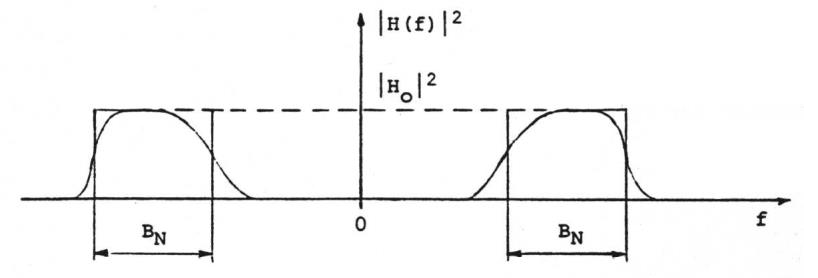
\includegraphics[scale = 1]{Valutazione della banda equivalente di rumore in un sistema.png}
\end{figure}

Se ci troviamo il caso uno spettro di rumore "colorato" come in figura (vale a dire a spettro non uniforme), 
$B_N$ non ha alcuna implicazione pratica diretta, in quanto lo spettro in uscita si ottiene dalla combinazione del modulo al quadrato della funzione di trasferimento e delle spettro di potenza in ingresso, 
ed è sempre il risultato del loro prodotto a dover essere integrato per ricavare la potenza in uscita. \newline 

In altre parole, per calcolare la potenza del rumore nel caso ideale del segnale rettangolare, abbiamo: 

{
    \Large 
    \begin{equation}
        \begin{split}
           <n^{2}>
           &=
           \frac{\eta}{2}
           \cdot
           \abs{H_0}^{2}
           \cdot
           2B 
           \\
           &=
           \eta B \abs{H_0}^2
        \end{split}
    \end{equation}
}

e possiamo dire che per un determinato $B_N$, 
la partenza del sistema equivalente è uguale a quello del sistema. \newline 

\newpage

\section{Temperatura equivalente di rumore di una rete 2-porte lineare}
\footnote{Slide del prof | Parametri di rumore sistema lineare | pag 2 - 4\\  
Appunti di Damiano| pag 2 - 4} 

Si consideri ora una rete 2-porte rumorosa, al cui ingresso si connette un resistore rumoroso a temperatura $T_i$. \newline 

All'uscita della rete 2-porte, si ha il rumore di ingresso amplificato (o attenuato) ed il rumore introdotto dalla rete 2-porte rumorosa. \newline 

Le fonti di rumore interne della rete sono, di regola, incorrelate rispetto al rumore generato dal resistore connesso in ingresso (i.e. sono indipendenti ed hanno covarianza nulla). \newline 

Pertanto, la potenza di rumore disponibile all'uscita della rete è uguale alla somma delle potenze di rumore disponibile dovute dalla: 

\begin{itemize}
    \item rumorosità della rete 
    \item rumore di ingresso amplificato (o attenuato) dalla rete
\end{itemize}

La stessa considerazione vale per le densità di potenza di rumore: 

{
    \Large 
    \begin{equation}
            \frac{\eta^{'}}{2} 
            = 
            G_d \frac{\eta}{2} + \frac{\delta \eta}{2} 
    \end{equation}
}

dove: 

\begin{itemize}
    \item $\frac{\eta^{'}}{2}$ è il segnale in uscita dalla rete 2-porte rumorosa, i.e. la densità di potenza in uscita
    \item $G_d$ è il rumore generato dal sistema lineare 
    \item  $\frac{\eta}{2}$ è il segnale di ingresso con rumore 
    \item $\frac{\delta \eta}{2}$ è la densità spettrale bilatera dovuta alla rete, i.e. la densità spettrale bilatera dovuta alla rete
\end{itemize}

Sapendo che: 

{
    \Large 
    \begin{equation}
        \begin{cases}
            \eta = K \cdot T_i 
            \\
            \eta^{'} = K \cdot T_u 
        \end{cases}
    \end{equation}
}

dove: 
\begin{itemize}
    \item $T_i$ è la temperatura in ingresso dal sistema lineare 
    \item $T_u$ è la temperatura in uscita dal sistema lineare
\end{itemize}

L'equazione della densità di potenza in uscita $ \frac{\eta^{'}}{2}$ diventa: 

{
    \Large 
    \begin{equation}
        \begin{split}
        \frac{\eta^{'}}{2} 
        &= 
        G_d \frac{\eta}{2} + \frac{\delta \eta}{2}     
       \\
       &\downarrow
       \\ 
       \frac{K \cdot T_u}{2} 
        &= 
        G_d \frac{K \cdot T_i}{2} + \frac{\delta \eta}{2}   
        \\
        &= 
        \frac{1}{2} (G_d \cdot K \cdot T_i + \delta \eta)
        \\     
        K \cdot T_u
        &= 
        G_d \cdot K \cdot T_i + \delta \eta
    \end{split}
    \end{equation}
}

Sapendo che la densità spettrale alla rete $\delta \eta$ si trova ad una temperatura $T_e$, possiamo esprimerla come: 

{
    \Large 
    \begin{equation}
        \delta \eta = G_d \cdot K \cdot T_e
    \end{equation}
}

l'espressione della densità di potenza in uscita $\frac{\eta^{'}}{2}$ possiamo continuarla ancora a semplificarla come: 

{
    \Large 
    \begin{equation}
        \begin{split}
        K \cdot T_u
        &= 
        G_d \cdot K \cdot T_i + \delta \eta
        \\
        &\downarrow
        \\
        K \cdot T_u
        &= 
        G_d \cdot K \cdot T_i + G_d \cdot K \cdot T_e
        \\
        &= 
        G_d \cdot K (T_i + T_e)
    \end{split}
    \end{equation}
}

$T_e$ prende il nome di "temperatura equivalente di rumore" della rete 2-porte. \newline 

$T_e$ rappresenta l'incremento di temperatura che occorre dare al resistore connesso all'ingresso della rete 2-porte supposta non rumorosa, 
per avere all'uscita la stessa densità di potenza disponibile di rumore che si ha con il generatore (di rumore) in ingresso a temperatura $T_i$ e rete 2-porte rumorosa. \newline 

O, spiegato in un'altra maniera, usando i sistemi equivalenti, la temperatura equivalente sposta tutto il rumore nell'ingresso, azzerando il rumore del sistema lineare. \newline 

Quindi, $T_e$ è un parametro caratteristico della rete e ne quantifica in maniera semplice ed esplicita la rumorosità. \newline 

È sufficiente aumentare di $T_e$ la temperatura di rumore in ingresso per poter considerare la rete 2-porte non rumorosa, 
pur ottenendo in uscita la stessa densità di potenza (e quindi la stessa potenza) di rumore del sistema reale. \newline 

$T_u$ rappresenta la temperatura equivalente di rumore complessiva in uscita, 
e può essere utilizzata per caratterizzare una cascata di reti 2-porte. \newline 

Quando si descrive la rumorosità del singolo dispositivo, si è soliti riferirsi alla sua sezione in ingresso, assegnando quindi direttamente il valore di $T_e$. \newline 


\newpage 

\section{Cifra di rumore di una rete 2-porte lineare}
\footnote{Slide del prof | Parametri di rumore sistema lineare | pag 3 - \\  
Appunti di Damiano| pag 3 - } 

In alternativa, alla temperatura equivalente di rumore, la rumorosità introdotta da una rete 2-porte può essere assegnata specificando la cosiddetta "cifra di rumore" (o "fattore di rumore") F. \newline 


F è definita come rapporto tra la densità di potenza disponibile di rumore in uscita da una rete 2-porte rumorosa, 
al cui ingresso sia connesso un generatore di rumore a temperatura standard $T_0$: 

{
    \Large 
    \begin{equation}
        \begin{split}
            T_0 
            &= 
            290 ^{\circ} K
            \\ 
            &= 
            (290 - 273.15) ^{\circ} C 
            \\
            &= 
            16.85 ^{\circ} C
            \\
            &\approx 
            17 ^{\circ} C
        \end{split}
    \end{equation}
}


e la densità di potenza disponibile di rumore dovuta all'amplificazione del rumore immesso in ingresso dal generatore. \newline

In formula, sulla base della notazione precedente: 

{
    \Large 
    \begin{equation}
        \begin{split}
            F 
            &= 
            \frac{\left. \eta^{'} \right|_{T_i = T_0}}{G_d \cdot K \cdot T_0 }
            \\
            &= 
            \frac{\left. G_d \cdot K (T_i + T_e) \right|_{T_i = T_0}}{G_d \cdot K \cdot T_0 }
            \\
            &=
            \frac{ G_d \cdot K (T_0 + T_e) }{G_d \cdot K \cdot T_0 }
            \\
            &=
            \frac{T_0 + T_e}{T_0}
            \\
            &= 
            \frac{T_0 (1 + \frac{T_e}{T_0})}{T_0}
            \\
            &= 
            1 + \frac{T_e}{T_0}
        \end{split}
    \end{equation}
}

Generalmente, e nella vita pratica, F cifra di rumore è sempre maggiore di 1, ma a livello teorico valgono le seguenti considerazioni teoriche. \newline 

La relazione di F con $T_e$ e $T_0$: 

{
    \Large 
    \begin{equation}
        F = 1 + \frac{T_e}{T_0}
    \end{equation}
}

stabilisce un legame esplicito tra temperatura equivalente di rumore e cifra di rumore della rete 2-porte, 
a conferma dell'equivalenza "operativa" delle due funzioni. \newline

In certi casi, può essere utile esplicitare il legame inverso, cioè: 

{
    \Large 
    \begin{equation}
        \begin{split}
        F &= 1 + \frac{T_e}{T_0}
        \\
        &\downarrow
        \\
        F - 1
        &= 
        \frac{T_e}{T_0}
        \\
        T_0 (F - 1)
        &=
        T_e 
        \\
        T_e 
        &=
        T_0 (F - 1)
        \end{split}
    \end{equation}
}

D'altro canto, moltiplicando numeratore e denominatore dall'equazione di F per la banda equivalente di rumore della rete 2-porte, 
la cifra di rumore F può anche essere riscritta come: 

{
    \Large 
    \begin{equation}
        \begin{split}
           F &= 1 + \frac{T_e}{T_0} 
           \\
           &\downarrow
           \\
           F &= \frac{<n^{'^{2}}>}{G_d \cdot <n^{2}>}
        \end{split}
    \end{equation}
}


dove: 

\begin{itemize}
    \item $<n^{2}>$ è la potenza di rumore dovuta al solo resistore a temperatura $T_0$ in ingresso (che abbiamo precedentemente calcolato) 
    \item $<n^{'^{2}}>$ è la potenza di rumore totale in uscita (comprensivo del contributo dovuto alla rete 2-porte)
\end{itemize}

Grazie a questa ultima relazione di F: 

{
    \Large 
    \begin{equation}
        F = \frac{<n^{'^{2}}>}{G_d \cdot <n^{2}>}
    \end{equation}
}

la cifra di rumore F esprime il rapporto tra il rumore in uscita dal 2-porte 
e quello che si avrebbe (sempre in uscita, stante la moltiplicazione di $<n^{2}>$ per $G_d$) 
se il 2-porte fosse ideale, cioè non introducesse alcuna rumorosità aggiuntiva. \newline 

È evidente che: 

{
    \Large 
    \begin{equation}
        F \ge 1
    \end{equation}
}

e, quanto più F risulta prossimo a 1, tanto più il comportamento del sistema lineare risulta migliore ai fini della rumorosità. \newline 

Tenendo conto che un segnale utile di potenza $S_i$ in ingresso si ritrova amplificato (o attenuato) e pari a $G_d \cdot S_i$ in uscita, 
si può semplificare ulteriormente numeratore e denominatore a secondo membro della funziona di F per $S_i$, ottenendo così: 

{
    \Large 
    \begin{equation}
        \begin{split}
            F &= \frac{<n^{'^{2}}>}{G_d \cdot <n^{2}>}
            \\
            &\quad
            \\
            &= \frac{S_i \cdot <n^{'^{2}}>}{S_i \cdot G_d \cdot <n^{2}>}
            \\
            &\quad
            \\
            &= \frac{\frac{S_i}{<n^{'^{2}}>}}{\frac{S_i \cdot G_d}{<n^{2}>} }
            \\
            &\quad
            \\
            &= \frac{\left( \frac{S}{N}\right)_{i}}{\left( \frac{S}{N}\right)_{u}}
            \\
            &\quad
            \\
            &= \frac{SNR_i}{SNR_u}
        \end{split}
    \end{equation}
}

dove: 

\begin{itemize}
    \item $SNR_i$ esprime il rapporto segnale-rumore in ingresso, in presenza del solo resistore a temperatura $T_0$
    \item $SNR_u$ esprime il rapporto segnale-rumore in uscita, includendo anche la rumorosità della rete a 2-porte
\end{itemize}

In condizioni ideali, per la rete a 2-porte, questo rapporto varrebbe 1, 
poiché segnale utile e rumore in ingresso verrebbero amplificati (o attenuati) della stessa quantità $G_d$. \newline 

In condizioni reali (cioè nel caso di un rete 2-porte rumorosa) F è sempre maggiore di 1 ed esprime il peggioramento nel rapporto segnale-rumore dovuto al 2-porte. \newline 

\newpage 

\section{Cifra di rumore di una rete 2-porte lineare e temperatura equivalente di rumore generalizzata}
\footnote{Slide del prof | Parametri di rumore sistema lineare | pag 4 - 5\\  
Appunti di Damiano| pag 4 - 5} 

È opportuno precisare che la definizione di cifra di rumore e temperatura equivalente di rumore si estende anche nel caso in cui la rumorosità introdotta dal sistema lineare è 
caratterizzata da uno spettro di potenza non uniforme e il guadagno disponibile è variabile con la frequenza. \newline 

In questo caso la F dipenderà dalla frequenza f, quindi passeremo al caso costante per ogni frequenza al caso generalizzato: 

{
    \Large 
    \begin{equation}
        \begin{split}
           F &= 1 + \frac{T_e}{T_0} 
           \\
           &\downarrow
           \\
        F(f) &= 1 + \frac{\delta \eta(f)}{\eta G_d (f)}
        \end{split}
    \end{equation}
}

Analogamente, possiamo generalizzare $T_e$ per ogni frequenza f: 

{
    \Large 
    \begin{equation}
        \begin{split}
        T_e 
        &=
        T_0 (F - 1) 
        \\
        &\downarrow
        \\
        T_e (f)
        &=
        T_0 \cdot [(F(f) - 1)] 
        \end{split}
    \end{equation}
}

Nell'ottica di caratterizzare con un unico numero la rete 2-porte, anche in questa situazione più generale, 
F(f) e $T_e (f)$ possono essere mediati sulla banda passante del rete 2-porte, 
in tal modo ottenendo: 

{
    \Large 
    \begin{equation}
        \begin{split}
            \overline{F}
            &= 
            \frac{\int_{-\infty}^{+\infty} F(f) \cdot G_d (f) df}{\int_{-\infty}^{+\infty} G_d (f) df}
            \\
            &\quad
            \\
            &= 
            \frac{1}{2 \abs{H_0}^{2} B_N} \int_{-\infty}^{+\infty} F(f) \cdot G_d (f) df
        \end{split}
    \end{equation}
}

e 

{
    \Large 
    \begin{equation}
        \begin{split}
            \overline{T_e}
            &=
            \frac{\int_{-\infty}^{+ \infty} T_e (f) \cdot G_d (f) df}{\int_{-\infty}^{+ \infty} G_d (f) df} 
            \\
            &\quad
            \\
            &=
            \frac{1}{2 \abs{H_0}^{2} B_N} \int_{-\infty}^{+ \infty} T_e (f) \cdot G_d (f) df
            \\
            &\quad
            \\
            &= 
            T_0 \cdot (\overline{F} - 1)
        \end{split} 
    \end{equation}
}

Le relazioni di $\overline{F}$ e $\overline{T_e}$ sono valide se: 

{
    \Large 
    \begin{equation}
        G_d (f) = \abs{H(f)}^{2}
    \end{equation}
}

\begin{tcolorbox}
    D'ora in poi non consideriamo la dipendenza dalla frequenza dei parametri per semplicità di notazione, 
    ma bisogna ricordarci che è possibile che esista per la teoria
\end{tcolorbox}

\newpage 

\section{2-porte in cascata}
\footnote{Slide del prof | Parametri di rumore sistema lineare | pag 5 - 6\\  
Appunti di Damiano| pag 5 - 6} 

Le espressioni sin qui introdotto sono sufficienti per descrivere la rumorosità di una singola rete 2-porte. \newline 

Cosa succede quando un certo numero di reti 2-porte vengono connessi in cascata come in figura? 

\begin{figure}[h]
    \centering
    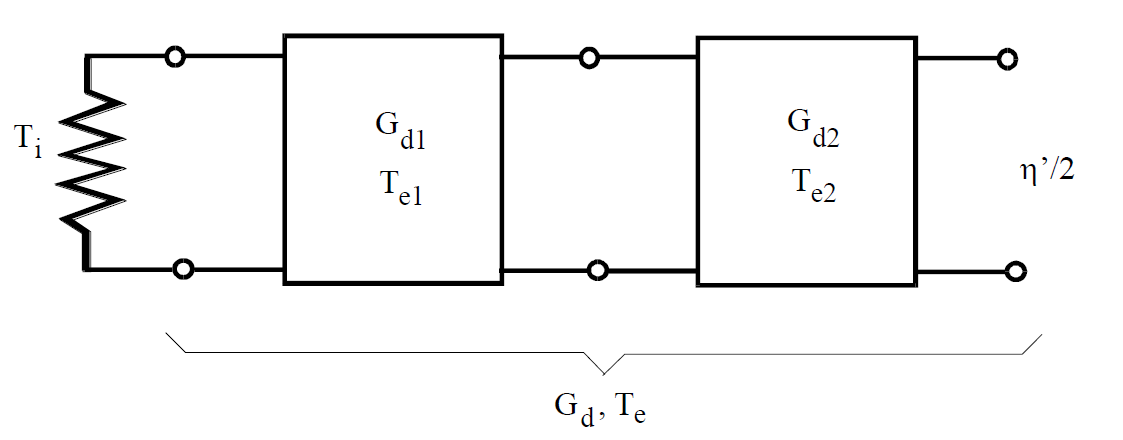
\includegraphics[scale = 0.8]{Cascata di reti 2-porte.PNG}
\end{figure}

La resistenza in ingresso, che schematizza una generica sorgente di rumore termico, si trova a temperatura $T_i$. \newline 

Ciascuna rete 2-porte è caratterizzata dal proprio guadagno disponibile, rispettivamente $G_{d1}$ e $G_{d2}$, e dalla propria temperatura equivalente di rumore, 
rispettivamente $T_{e1}$ e $T_{e2}$. \newline 

Se: 

{
    \Large 
    \begin{equation}
        G_{d1} > 1
    \end{equation}
}

la rete a 2-porte viene identificato come amplificatore. \newline 

Se: 

{
    \Large 
    \begin{equation}
        G_{d1} < 1
    \end{equation}
}

la rete a 2-porte viene identificato come attenuatrice. \newline 

Considerando solo il primo sistema lineare (quello a sinistra della figura), 
possiamo esprimere la temperatura di rumore complessiva $T_{u1}$ del primo sistema lineare 
(come studiato nelle scorse sezioni) come: 

{
    \Large 
    \begin{equation}
        \begin{split}
            K \cdot T_{u1} &= G_d \cdot K \cdot (T_i + T_{e1})
            \\
            T_{u1} &= G_d \cdot (T_i + T_{e1})
        \end{split}
    \end{equation}
}

$T_{u1}$ può essere interpretata come la temperatura equivalente in ingresso alla seconda rete 2-porte, 
in uscita dalla quale si avrà allora: 

{
    \Large 
    \begin{equation}
        \begin{split}
            T_{u2}
            &= 
            G_{d2} \cdot (T_{u1} + T_{e2})
            \\
            &= 
            G_{d2} \cdot [G_{d1} (T_i + T_{e1}) + T_{e2}]
            \\
            &=
            G_{d1} \cdot G_{d2} \cdot T_i 
            + 
            G_{d1} \cdot G_{d2} \cdot T_{e1} 
            + 
            G_{d2} \cdot T_{e2}
        \end{split}
    \end{equation}
}


Tenendo conto che il guadagno disponibile della cascata $G_d$ vale: 

{
    \Large 
    \begin{equation}
        \begin{split}
            G_d &= G_{d1} \cdot G_{d2}
            \\ 
            &\updownarrow
            \\
            G_{d2} &= \frac{G_d}{G_{d1}}
        \end{split}
    \end{equation}
}

e che, per definizione di temperatura equivalente, si deve poter scrivere: 

{
    \Large 
    \begin{equation}
        T_{u2} = G_d \cdot (T_i + T_e)
    \end{equation}
}

con $T_e$ temperatura equivalente della cascata, per confronto si ricava: 

{
    \Large 
    \begin{equation}
        \begin{split}
            T_{u2}
            &=
            G_{d1} \cdot G_{d2} \cdot T_i 
            + 
            G_{d1} \cdot G_{d2} \cdot T_{e1} 
            + 
            G_{d2} \cdot T_{e2}
            \\
            G_d \cdot (T_i + T_e)
            &=
            G_d \cdot T_i
            + 
            G_d \cdot T_{e1}
            + 
            G_{d2} \cdot T_{e2}
            \\
            G_d \cdot T_i + G_d \cdot T_e 
            &=
            \\
            G_d \cdot T_e 
            &=
            G_d \cdot T_{e1} + G_{d2} \cdot T_{e2}
            \\
            &= 
            G_d \cdot T_{e1} + \frac{G_d}{G_{d1}} \cdot T_{e2}
            \\
            &= 
            G_d \cdot (T_{e1} + \frac{T_{e2}}{G_{d1}})
            \\
            T_e
            &=
            T_{e1} + \frac{T_{e2}}{G_{d1}}
        \end{split}
    \end{equation}
}

La formula di $T_e$ appena scritta esplicita che la temperatura equivalente di due sistemi lineari in cascata 
si ottiene sommando alla temperatura equivalente del primo stadio $T_{e1}$ la temperatura equivalente del secondo stadio $T_{e2}$ per il guadagno del primo stadio $G_{d1}$. \newline 

Inoltre, la formula di $T_e$ fornisce un'altra informazione quantitativa estremamente importante: 
dovendo scegliere la collocazione relativa, ad esempio, di due stadi amplificatori, 
tendenzialmente si metterà in testa quello meno rumoroso, 
in quanto la rumorosità dell'altro stadio (maggiore) sarà ridotta del fattore $G_{d1}$. \newline 

Se il primo stadio è un attenuatore, cioè $G_{d1} < 1$, la rumorosità del secondo stadio verrebbe amplificata. \newline 

In questo caso, è meglio, se possibile, porre l'attenuatore dopo l'amplificatore. \newline 

È per questo motivo per cui il pre-amplificatore, 
per un sistema di ricezione televisivo, 
viene posto a contatto con l'antenna e prima del cavo che porta il segnale al cinescopio (la cosiddetta "discesa d'antenna"). \newline 

\newpage 

\subsection{Cifra di rumore e temperatura equivalente di rumore di una cascata di reti 2-porte lineare }
\footnote{Slide del prof | Parametri di rumore sistema lineare | pag 6 - \\  
Appunti di Damiano| pag 6 - } 

In generale, la disposizione relativa dei componenti di una cascata va ottimizzata, 
tenendo conto dei valori relativi del guadagno e della temperatura equivalente di rumore, 
in modo da minimizzare la formula di $T_e$: 

{
    \Large 
    \begin{equation}
            T_e
            =
            T_{e1} + \frac{T_{e2}}{G_{d1}}
    \end{equation}
}

La proceduta che ha consentito di ricavare la temperatura equivalente di rumore per una coppia di reti 2-porte, 
può essere estratta ad un numero n qualsiasi di sistemi lineari connessi in cascata. \newline 

La temperatura equivalente di rumore globale si ottiene dalla seguente espressione: 

{
    \Large 
    \begin{equation}
        T_e 
        = 
        T_{e1}
        + 
        \frac{T_{e2}}{G_{d1}}
        + 
        \frac{T_{e3}}{G_{d1} \cdot G_{d2}}
        + 
        \dots
        +
        \frac{T_{en}}{G_{d1} \cdot G_{d2} \cdot \dots \cdot G_{dn-1}}
    \end{equation}
}

Una eguale espressione compatta, sapendo il legame tra temperatura equivalente e cifra di rumore, si ricava come: 

{
    \Large 
    \begin{equation}
        F 
        = 
        F_{1}
        + 
        \frac{F_{2} - 1}{G_{d1}}
        + 
        \frac{F_{3} - 1}{G_{d1} \cdot G_{d2}}
        + 
        \dots
        +
        \frac{F_{n} - 1}{G_{d1} \cdot G_{d2} \cdot \dots \cdot G_{dn-1}}
    \end{equation}
}

Questa ultima formula di F è nota come "formula di Friis". \newline 

Grazie alla formula di Friis, possiamo fare le stesse considerazioni sulla cascata delle n porte partendo dalla cascata dei due sistemi lineari. \newline 

La rumorosità del primo stadio, qui espressa da $F_1$, è, in generale, la più importante nell'ambito della cascata (e va dunque adeguatamente controllata). \newline 

Si è già detto in precedenza che, uno o più stadi della cascata, possono, in realtà, presentare un comportamento da attenuatore, nel caso in cui: 

{
    \Large 
    \begin{equation}
        G_d = \frac{1}{A_d}  < 1
    \end{equation}
}

e, più che il guadagno, risulta significativo considerare l'attenuazione disponibile $A_d$, che risulta maggiore di 1. \newline 

Frequentemente, sia $G_d$ che $A_d$, sono espresse in unità logaritmiche (dB), in cui avere un numero 
in unità assolute, maggiore di 1 (o minore di 1), corrisponde a una misura in dB positiva (o negativa). \newline 

\newpage 

\section{2-porte attenuatrice: rumorosità}
\footnote{Slide del prof | Parametri di rumore sistema lineare | pag 6 - 7\\  
Appunti di Damiano| pag 6 - 7} 

È interessante chiedersi quanto valga la rumorosità di una rete 2-porte attenuatrice. \newline 

Essa è, tipicamente, realizzata utilizzando un attenuatore resistivo, 
in cui l'attenuazione è il risultato della dissipazione di potenza elettrica immensa nelle resistenze. \newline 

Dal punto di vista grafico, possiamo schematizzarlo in questa maniera: 

\begin{figure}[h]
    \centering
    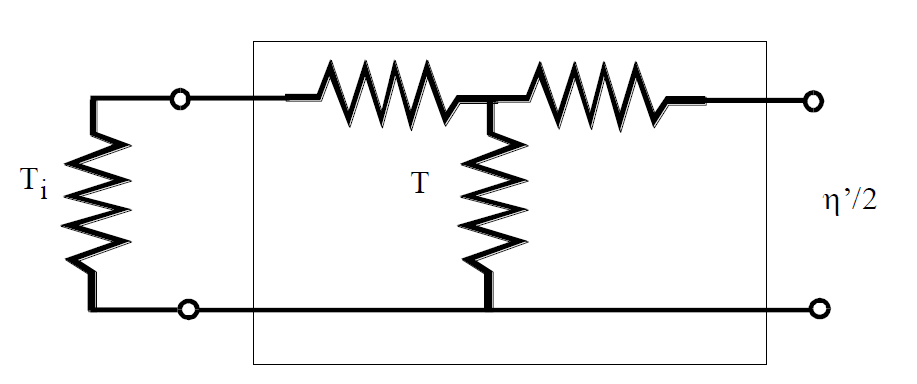
\includegraphics[scale = 0.8]{2-porte attenuatrice.PNG}
\end{figure}

Si suppone che l'attenuatore sia collegato in ingresso ad un generatore di rumore a temperatura $T_i$, 
in generale diversa dalla temperatura T dell'attenuatore. \newline 

Si può pensare che la densità di potenza disponibile nel sistema considerato sia divisa in due parti: 

\begin{itemize}
    \item la prima, pari a $K \cdot \frac{T_i - T}{2}$ è relativa all'eccesso di temperatura $T_i$ rispetto a T 
    \item la seconda, pari a $K \cdot \frac{T}{2}$ sarebbe invece, la sola densità di potenza disponibile nel caso in cui il resistore fosse alla stessa temperatura T dell'attenuatore
\end{itemize}

Se: 

{
    \Large 
    \begin{equation}
        T_i = T
    \end{equation}
}

l'insieme del resistore esterno all'attenuatore e dei resistori interni costituirebbero un'unica resistenza a temperatura T. \newline 

La densità spettrale di potenza di rumore $<P_n>$ disponibile è indipendente dal valore della resistenza. \newline  

Se si considera solo f positive, $<P_n>$ sarà uguale a: 

{
    \Large 
    \begin{equation}
        \begin{split}
            <p_n> 
            &= 
            \int_{0}^{+B} \eta(f) df 
            \\
            &= 
            K \cdot T
        \end{split}
    \end{equation}
}

Se si considera solo f positive e f negative, $<P_n>$ sarà uguale a: 

{
    \Large 
    \begin{equation}
        \begin{split}
            <p_n> 
            &= 
            \int_{-B}^{+B} \eta(f) df 
            \\
            &= 
            K \cdot \frac{T}{2}
        \end{split}
    \end{equation}
}

L'incremento di R dovuto all'attenuatore, non modificherebbe in alcun modo la rumorosità in ingresso. \newline 

Il contributo $ K \cdot \frac{T}{2}$ resta tale qualunque sia la sezione in cui si colloca (in particolare in uscita dell'attenuatore). \newline 

Il contributo $ K \cdot \frac{T_i - T}{2}$, invece, che è relativo all'eccesso di temperatura del resistore in ingresso, 
deve essere moltiplicato per il guadagno, 
ovvero, diviso per l'attenuazione disponibile. \newline 

In definitiva, la densità di potenza di rumore nella sezione di uscita vale: 

{
    \Large 
    \begin{equation}
        \begin{split}
            \frac{\eta^{'}}{2}
            &= 
            \frac{K \cdot T}{2}
            +
            \frac{K \cdot (T_i - T)}{2 \cdot A_d}
            \\
            &= 
            \frac{K \cdot T_i}{2 \cdot A_d}
            + 
            \frac{K \cdot T}{2}
            \cdot 
            \left( 1 - \frac{1}{A_d}\right)
        \end{split}
    \end{equation}
}

Indicando con $T_e$ la temperatura equivalente dell'attenuatore, 
possiamo riscrivere la densità di potenza di rumore nella sezione di uscita come: 

{
    \Large 
    \begin{equation}
        \begin{split}
            \frac{\eta^{'}}{2}
            &= 
            \frac{K \cdot (T_i - T_e)}{2 \cdot A_d}
            \\
            &= 
            \frac{K \cdot T_i}{2 \cdot A_d}
            + 
            \frac{K \cdot T_e}{2 \cdot A_d}
        \end{split}
    \end{equation}
}

Uguagliando le due formule di $\frac{\eta^{'}}{2}$ e svolgendo alcuni passi algebrici, 
possiamo ricavare $T_e$ come: 

{
    \Large 
    \begin{equation}
        T_e = T \cdot (A_d - 1)
    \end{equation}
}

Questa ultima espressione di $T_e$ esprime la temperatura equivalente di un attenuatore resistivo. \newline 

Di conseguenza, la cifra di rumore che corrisponde ad un attenuatore resistivo, vale: 

{
    \Large 
    \begin{equation}
        F = 1 + \frac{T}{T_0} \cdot (A_d - 1)
    \end{equation}
}

Nel caso particolare, ma importante, in cui l'attenuatore si trovi a temperatura standard $T_0$, 
la sua cifra di rumore uguaglia l'attenuazione disponibile, cioè: 

{
    \Large 
    \begin{equation}
        F = A_d
    \end{equation}
}

Perciò, maggiore è l'attenuazione, maggiore è la rumorosità introdotta dall'attenuatore. \newline 

Le considerazioni svolte per gli attenuatori resistivi valgono per tronchi di guida d'onda o di linee che introducono attenuazione. \newline 

\newpage

\section{Rumorosità di un sistema ricevente radio}
\footnote{Slide del prof | Parametri di rumore sistema lineare | pag 8 \\  
Appunti di Damiano| pag 8} 

Nel caso in cui si debba caratterizzare la rumorosità di un sistema ricevente per collegamenti radio, 
in cui l'insieme degli apparati che costituiscono il ricevitore (cavi, amplificatori, mixer, $\dots$) sia chiuso in ingresso dall'antenna ricevente, 
la temperatura di ingresso $T_i$ deve essere assunta la temperatura di antenna $T_A$. \newline 

La somma della temperatura equivalente del radioricevitore prende il nome di temperatura di sistema $T_S$, 
che si ottiene come: 

{
    \Large 
    \begin{equation}
        T_S = T_A + T_e
    \end{equation}
}

$T_A$ non è la temperatura fisica dell'antenna, ma dipende da dove viene puntata. \newline 

Quando $T_A \approx T_0$, $T_S$ si può esprimere come: 

{
    \Large 
    \begin{equation}
        T_S \approx T_0 \cdot F_r
    \end{equation}
}

dove $F_r$ è la cifra di rumore del ricevitore. \newline 

\newpage 

\section{Conclusioni riguardo la temperatura equivalente}
\footnote{Slide del prof | Parametri di rumore sistema lineare | pag 8\\  
Appunti di Damiano| pag 8} 

In chiusura, si vuole ribadire l'importanza applicativa della definizione di temperatura equivalente (o cifra di rumore a cui essa è legata). \newline 

Trasferendo la rumorosità dovuta alla rete 2-porte (o alla cascata di reti 2-porte) in un incremento della temperatura che schematizza la rumorosità in ingresso, 
essa consente di considerare la rete stessa non rumorosa. \newline 

Come conseguenza, il rapporto segnale-rumore è costante in qualunque sezione del sistema lineare in cui venga calcolato. \newline 

Segnale utile e rumore sono trattati allo stesso modo da blocchi ideali. \newline 

Ovviamente, ciò che resta invariato è un rapporto segnale-rumore in cui la potenza di rumore è onnicomprensiva e tiene conto, in qualunque sezione, anche della rumorosità dei blocchi posti a valle. \newline 

D'altro canto, è questa la rumorosità che interessa ai fini del dimensionamento del sistema e della valutazione delle sua prestazioni. \newline 

Una potenza di rumore che escluda alcuni contributi può essere utile per capire la dinamica del disturbo, 
ma non ha alcuna utilità della caratterizzazione del sistema complessivo. \newline 

Il rapporto segnale-rumore può essere riferito e calcolato in una qualunque sezione. \newline 

Tipicamente ci si colloca in ingresso, ma ciò non rappresenta una scelta obbligata. \newline 

Il fatto che l'SNR resti invariato nel sistema equivalente non implica che la potenza di segnale utile o quella di rumore, considerati individualmente, 
restino pure invariati. \newline 

Al contrario, la potenza S, ad esempio, viene moltiplicata, nel passaggio dall'ingresso all'uscita, per il guadagno disponibile $G_d$, 
lo stesso si verifica per la potenza di rumore. \newline 

Di conseguenza, anche la temperatura equivalente della cascata (cui la potenza di rumore risulta proporzionale) 
può essere riportata in una qualunque sezione, 
semplicemente moltiplicando o dividendo per gli opportuni guadagni (dei blocchi che separano le sezioni considerate). \newline 

\newpage 

\section{Da segnale analogico a segnale digitale}
\footnote{Slide del prof | Parametri di rumore sistema lineare | pag 13\\  
Appunti di Damiano| pag 13} 

In un sistema analogico, le potenze di rumore introdotte dalle singole tratte, supposte tra loro indipendenti, si sommano. \newline 

La potenza di rumore, in analogico, è approssimativamente ad n volte il risultato che si ottiene considerando la tratta singola. \newline 

Ciò si traduce in una significativa degradazione del rapporto segnale-rumore il cui valore, 
è inversamente proporzionale al numero delle tratte considerate. \newline 

Il rapporto segnale rumore è il parametro di merito da utilizzare per esprimere la qualità di un segnale analogico. \newline 

La situazione è radicalmente diversa quando si considera un sistema numerico (sempre organizzato in n tratte). \newline 

Qui il parametro di merito diventa la probabilità di errore e si dimostra che (sarà dimostrato nei successivi capitoli) che, in questo caso, 
sono proprio le probabilità di errore a dover essere sommate, nella cascata di n tratte, per ottenere la probabilità di errore complessiva che influenza l'intero collegamento. \newline 

Questo risultato, peraltro, è conseguenza di una diversa organizzazione di sistema di trasmissione. \newline 

Mentre nel caso analogico i ripetitori posti alla fine di ogni tratta sono essenzialmente degli amplificatori, 
nel caso numerico può essere più conveniente effettuare ad ogni stazione intermedia una "rigenerazione" del segnale, 
cioè estrarre i dati ed effettuare una nuova trasmissione nella tratta successiva. \newline 

È proprio questa procedura che consente di evitare l'accumulazione dei disturbi. \newline 

Per fissare le idee, si può supporre che, in ciascuna tratta, la trasmissione avvenga con le modalità di un canale binario simmetrico caratterizzato da una probabilità di transizione errata 
sul simbolo binario uguale a p. \newline 

Si ha, allora, un errore finale sul simbolo trasmesso se avviene in un numero dispari di tratte: 
con un numero pari di errori: infatti, si ha una compensazione e, in uscita, si riottiene il simbolo corretto. \newline 

Ad esempio se si ha il simbolo 1, se le tratte sono pari, il simbolo ritorna a 1; 
se le tratte sono dispari, il simbolo o può essere 1 o 0, che è diverso da 1. \newline 

Ma la probabilità di errore su 3, 5, $\dots$ tratte è in genere (se p è piccola) trascurabile, 
rispetto alla probabilità di sbagliare su una sola delle n tratte. \newline 

Quest'ultima probabilità, che approssima, nel senso precisato, la probabilità di errore globale $P_{E}^{n}$ vale: 

{
    \Large 
    \begin{equation}
        \binom{n}{1}p(1-p)^{n-1} 
        \approx 
        n \cdot p 
        \approx 
        P_{E}^{(n)}
    \end{equation}
}

Questa ultima formula esplicita che la probabilità di errore si sommano nella cascare di n tratte. \newline 

Questa formula è nettamente favorevole rispetto a quella valida nel caso di sistema analogici. \newline 

In particolare, tenendo conto che la probabilità di errore decresce molto velocemente al crescere del rapporto segnale-rumore (tipicamente con legge esponenziale), 
si verifica che, aumentando anche considerevolmente il numero di tratte la variazione corrispondente nel rapporto segnale-rumore, si mantiene costante. \newline 

\newpage 

\subsection{Calcolo numerico di n tratte per un segnale analogico rispetto al segnale digitale}
\footnote{Slide del prof | Parametri di rumore sistema lineare | pag 13\\  
Appunti di Damiano| pag 13} 

Ad esempio, nel caso di un segnale analogico, considerando: 

{
    \Large 
    \begin{equation}
        n = 10
    \end{equation}
}

tratte, il rapporto segnale e rumore deve essere aumentato di 10 dB per mantenere la qualità che si avrebbe con una tratta singola. \newline 

Considerando invece un segnale numero in banda base con forma d'onda anti-podali, 
e volendo conseguire una probabilità di errore globale: 

{
    \Large 
    \begin{equation}
        P_{E}^{(n)} = 10^{-5}
    \end{equation}
}

sappiamo che, considerando $n = 1$: 

{
    \Large 
    \begin{equation}
        \binom{n}{1}p(1-p)^{n-1} 
        \approx 
        n \cdot p 
        \approx 
        P_{E}^{(n)}
    \end{equation}
}

quindi: 


{
    \Large 
    \begin{equation}
        \begin{split}
        n \cdot p 
        &\approx 
        P_{E}^{(n)} 
        \\
        &\downarrow
        \\
        1 \cdot p 
        &\approx 
        P_{E}^{(n)}
        \\
        p 
        &=
        P_{E}^{(n)}
        = 
        10^{-5} 
        \end{split} 
    \end{equation}
}

se invece $n = 10$: 

{
    \Large 
    \begin{equation}
        \begin{split}
        n \cdot p 
        &\approx 
        P_{E}^{(n)} 
        \\
        &\downarrow
        \\
        n \cdot p 
        &\approx 
        P_{E}^{(n)}
        =
        10^{-5}  
        \\
        p 
        &=
        \frac{P_{E}^{(n)}}{n}
        = 
        \frac{10^{-5}}{10}
        = 
        10^{-6}
        \end{split} 
    \end{equation}
}


Come si dimostrerà, trattando la qualità delle trasmissioni numeriche, 
in particolare per il caso di segnali antipodali, 
il rapporto segnale-rumore quando si passa da n = 1 a n = 10, 
deve essere aumentato di circa 1 dB. \newline 

Un valore significativamente minore rispetto a quanto richiesto nel caso di collegamento analogico. \newline 

\newpage 





\chapter{Modulazioni analogiche}

\begin{figure}[h]
    \centering
    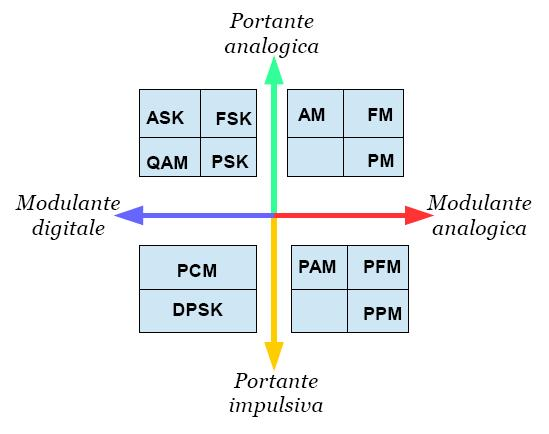
\includegraphics[scale = 1]{classificazione_modulazioni.jpg}
\end{figure}

\newpage 

\section{Rappresentazioni di segnali in modulazione}
\footnote{Slide del prof | Modulazioni analogiche | pag 1 - 2 \\  
Appunti di Damiano| pag 1 - 2 \\
Appunti | Modulazioni analogiche | pag 1 - 2 \\
Appunti | 2025-02-28 | pag 2
} 

Un significativo esempio di applicazione della Teoria dei Segnali, si rinviene nella rappresentazione 
nel dominio del tempo e della frequenza dei segnali modulati. \newline 

Nell'ambito delle telecomunicazioni, il termine modulazione sta ad indicare l'operazione (o in generale, il complesso delle operazioni) 
che consente di trasferire l'informazione da trasmettere (chiamato segnale modulante) in uno o più parametri di un segnale di portante. \newline 

Il risultato di questo "trasferimento" è un nuovo segnale chiamato segnale modulato. \newline 

Possiamo schematizzare la modulazione in questa maniera: 

\begin{figure}[h]
    \centering
    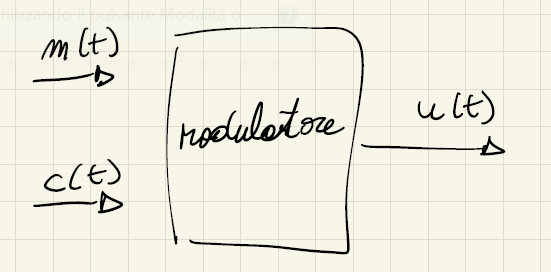
\includegraphics[scale = 0.5]{Schema della modulazione.PNG}
\end{figure}

dove: 

\begin{itemize}
    \item  m(t) è il segnale modulante, dall'inglese modulating signal 
    \item c(t) è il segnale portante, dall'inglese carrier
    \item u(t) è il segnale modulato
\end{itemize}

Il segnale modulato è quello più idoneo alla trasmissione nel canale e può essere inviato nel canale con le modalità che si sono scelte a priori. \newline

Benché la modulazione possa essere riferita anche a segnali passa-basso (ad esempio nel mixer di uno strumento musicale), 
"storicamente" la modulazione nasce per trasformare segnali passa-basso (cioè in banda base) in segnali passa-banda (quindi che dalla banda base li troveremo in alta frequenza, i.e. traslati nello spettro). \newline 

Questa traslazione in frequenza è dovuta principalmente a tre punti: 

\begin{enumerate}
    \item Necessità di utilizzare antenne di dimensioni ridotte nelle trasmissioni radio: la frequenza di trasmissione dipende dalla lunghezza d'onda del segnale, che deve essere uguale alle dimensioni dell'antenna 
    \item Necessità di utilizzare al meglio la funzione di trasferimento del canale trasmissivo: la modulazione permette di modulare il segnale modulante, che si trova in BB (Banda Base) in intervalli di frequenze in cui il canale distorce meno il segnale 
    \item Necessità di trasmettere contemporaneamente più segnali che originariamente occupano lo stesso intervallo di frequenze: si pensi ad esempio al segnale musicale in BB che deve essere trasmesso nella radio commerciale 
\end{enumerate}

\begin{tcolorbox}
    È vero che adesso esistono i podcast, ma ricordati di ascoltare un po' la radio. \newline 

    Prima di diventare anche tu zanzaroso e accendere la radio per ascoltare La Zanzara con David Parenzo e Cruciani, 
    ascoltati altri programmi interessanti nel palinsesto della "Radio di Confindustria". \newline 
    
    Te ne consiglio due dal lunedì al venerdì: 
    \begin{itemize}
        \item Due di Denari, con Mauro Meazza e Debora Rosciani, dalle 11 alle 12 \\ \url{https://www.radio24.ilsole24ore.com/conduttori/debora-rosciani/programmi/due-denari} 
        \item Focus economia, con Sebastiano Barisoni, dalle 17 alle 18:30, specialmente l'immancabile episodio di venerdì con la "poco invidiabile classifica degli sprechi" \\ \url{https://www.radio24.ilsole24ore.com/programmi/focus-economia} 
    \end{itemize}

    Prima il dovere e poi il piacere. \newline 

    AVANTI TIGRE
\end{tcolorbox}

Oltre ai vantaggi appena elencati, ce ne sono molti altri che non stiamo qui ad elencare. \newline 

Un grosso vantaggio della modulazione è l'allargamento dello spettro, che permette di migliorare l'immunità della trasmissione ai diversi agenti di disturbi di norma presenti. \newline 

Generalmente il disturbo principale che avremo a che fare è il nostro "caro amico" rumore termico. \newline 

\begin{tcolorbox}
   Al nostro caro amico rumore termico gli dedico questa canzone: \newline
   
   Toy Story - Un amico in me \\
   \url{https://youtu.be/0O_WONxv5p0?si=Hp4Aiu4OBY5xu6pT}
\end{tcolorbox}

\newpage 

\section{Modulazione analogica di una portante sinusoidale}
\footnote{Slide del prof | Modulazioni analogiche | pag 3 \\  
Appunti di Damiano| pag 3 \\
Appunti | Modulazioni analogiche | pag 3 \\
Appunti | 2025-02-28 | pag 3
} 

Un segnale c(t) (carrier, cioè segnale di portante) sinusoidale può essere descritto dalla seguente equazione: 

{
    \Large 
    \begin{equation}
        c(t) = A_c \cdot \cos(2 \pi f_c t + \phi_c)
    \end{equation}
}

dove: 

\begin{itemize}
    \item $A_c$ è l'ampiezza della sinusoide 
    \item $f_c$ è la frequenza, cioè l'inverso del periodo T di una sinusoide 
    \item t è il tempo 
    \item $\phi_c$ è la fase iniziale
\end{itemize}

Da un punto di vista grafico, nel tempo t possiamo visualizzare i parametri della sinusoide con la seguente figura: 

\begin{figure}[h]
    \centering
    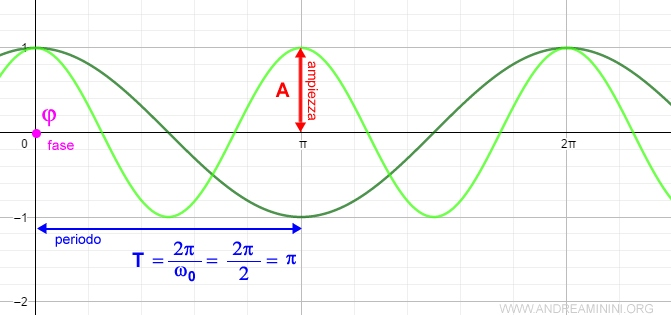
\includegraphics[scale = 0.5]{segnale-sinusoidale-aumento-freq.jpg}
\end{figure}

oppure nel piano fasoriale (che ci sarà molto utile nelle future trattazioni): 

\begin{figure}[h]
    \centering
    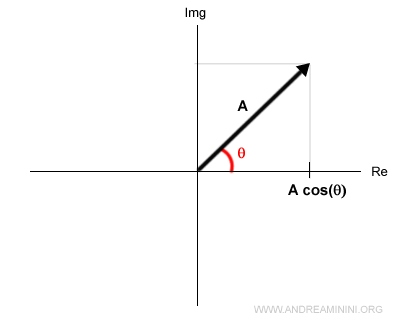
\includegraphics[scale = 0.5]{fasore-esempio-sinusoide.jpg}
\end{figure}

dove: 

\begin{itemize}
    \item $A \cdot \cos(\theta)$ è la proiezione del vettore $\overrightarrow{A}$ sull'asse reale 
    \item $A \cdot \sin(\theta)$ è la proiezione del vettore $\overrightarrow{A}$ sull'asse immaginario 
\end{itemize}

\newpage

Con la seguente figura: 

\begin{figure}[h]
    \centering
    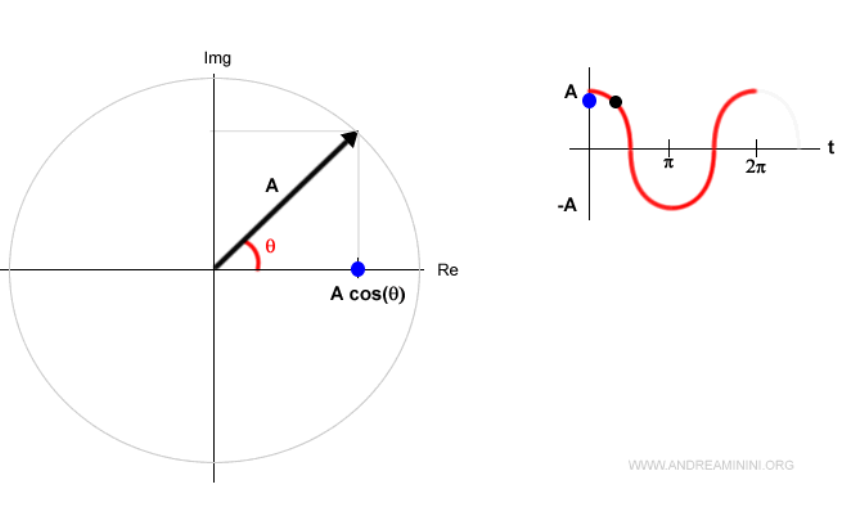
\includegraphics[scale = 0.5]{Piano fasoriale e andamento nel tempo.PNG}
\end{figure}

possiamo capire la relazione tra l'andamento nella sinusoide nel tempo e il piano fasoriale. \newline 

\begin{tcolorbox}
    Sembra banale ripassare i concetti basilari di una sinusoide, ma meglio essere tutti sulla stesso punto di inizio che far finta di capire qualcosa. \newline 
    
    Per approfondire: \\
    \url{https://www.andreaminini.org/telecomunicazioni/il-segnale-sinusoidale}
\end{tcolorbox}

Ritornando alla formula di c(t): 

{
    \Large 
    \begin{equation}
        c(t) = A_c \cdot \cos(2 \pi f_c t + \phi_c)
    \end{equation}
}

è evidente che è caratterizzata da tre gradi di libertà (cioè parametri che possiamo cambiare): 

\begin{itemize}
    \item l'ampiezza $A_c$ 
    \item la frequenza $f_c$ 
    \item la fase iniziale $\theta_c$
\end{itemize}

\begin{tcolorbox}
    Rispetto al corso di Segnali Determinati e Aleatori, o Teoria dei segnali per quelli del vecchio ordinamento, 
    in questo corso si predilige l'uso della frequenza f piuttosto che dei radianti $\omega$. \newline
    
    La relazione tra radianti e frequenza è la seguente: 

    {
        \Large 
        \begin{equation}
            \omega = 2 \pi f
        \end{equation}

    }
    
\end{tcolorbox} 


Questi gradi di libertà sono costanti e invariabili per qualunque istante di tempo nel segnale c(t). \newline 

Con la modulazione si vuole far dipendere uno o più di questi parametri di c(t), detto segnale di portante, a dei parametri di un altro segnale m(t), 
detto appunto segnale modulante. \newline 

Si parlerà di: 

\begin{itemize}
    \item modulazione di ampiezza (Amplitude Modulation o AM) quando l'ampiezza $A_c$ verrà resa dipendente da m(t)
    \item modulazione in frequenza (Frequency Modulation o FM) quando la frequenza $f_c$ verrà resa dipendente da m(t)
    \item modulazione di fase (Phase Modulation o PM) quando la fase iniziale $\phi_c$ verrà resa dipendente da m(t)
\end{itemize}

In realtà, si avrà modo di precisare che sia la modulazione di frequenza e sia la modulazione di fase sono tra loro intimamente legate: 
per cui, ove si realizzi una modulazione di frequenza, si realizza anche una modulazione di fase e viceversa. \newline 

Per questo motivo, sia la modulazione di fase che di frequenza, possono essere definite anche come modulazioni angolari, 
perché il segnale modulante agisce sull'angolo della funzione sinusoide. \newline 

\newpage 

\section{Modulazione di ampiezza}
\footnote{Slide del prof | Modulazioni analogiche | pag 3 \\  
Appunti di Damiano| pag 3 \\
Appunti | Modulazioni analogiche | pag 3 \\
Appunti | 2025-02-28 | pag 3
} 

Ritornando al segnale c(t): 

{
    \Large 
    \begin{equation}
        c(t) = A_c \cdot \cos(2 \pi f_c t + \phi_c)
    \end{equation}
}

andiamo a spiegare diverse modulazioni in cui l'ampiezza $A_c$ verrà resa dipendente da m(t), segnale modulante. \newline 

\newpage 

\subsection{Banda Laterale Doppia Portante Soppressa (DSB-SC)}
\footnote{Slide del prof | Modulazioni analogiche | pag 3 - 6\\  
Appunti di Damiano| pag 3 - 6\\
Appunti | Modulazioni analogiche | pag 3 - 6 \\
Appunti | 2025-02-28 | pag 3 - 5 \\
Appunti | 2025-03-03 | pag 2
} 

Nella modulazione di ampiezza con banda laterale doppia portante soppressa (o più frequentemente DSB-SC: Double Side Band - Suppressed Carrier), 
il segnale modulato u(t) è ottenuto semplicemente moltiplicando il segnale c(t) per il segnale modulante m(t). \newline 

In formula: 

{
    \Large 
    \begin{equation}
        \begin{split}
            u (t) 
            &= 
            m(t) \cdot c(t)
            \\
            &=
            m(t) \cdot \left[ A_c \cdot \cos(2 \pi f_c t + \phi_c) \right]
            \\
            &= 
            \left[A_c \cdot m(t) \right] \cdot \cos(2 \pi f_c t + \phi_c)
        \end{split}
    \end{equation}
}

Un esempio si segnale modulato u(t): 

{
    \Large 
    \begin{equation}
        u (t) 
        = 
        \left[A_c \cdot m(t) \right] \cdot \cos(2 \pi f_c t + \phi_c)
    \end{equation}
}

partendo da un segnale m(t) modulante è raffigurato nelle seguenti figure: 

\begin{figure}[h]
    \centering
    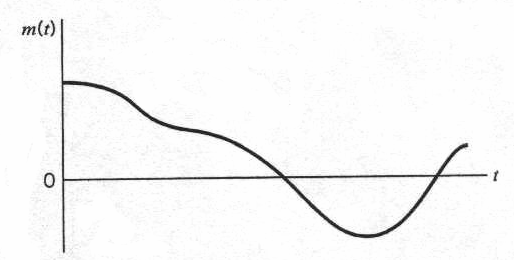
\includegraphics[scale = 0.8]{Segnale modulante.png}
    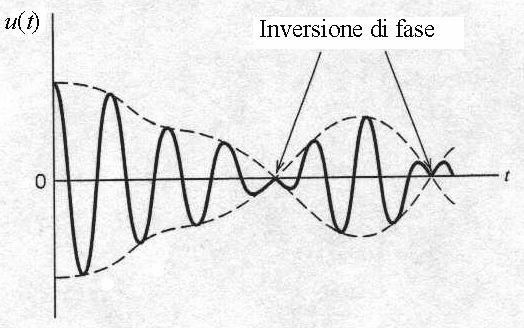
\includegraphics[scale = 0.8]{Segnale modulato in AM.png}
\end{figure}

È interessante l'inversione di fase del segnale modulato in corrispondenza dei passaggi per lo zero del segnale modulante. \newline 

Inoltre, nella figura di u(t), è tratteggiato l'andamento di m(t). \newline 

Utilizzando le proprietà della trasformata di Fourier, cioè quella della trasformazione in frequenza e quella del prodotto,
u(t) ha una semplice rappresentazione in frequenza: 

{
    \Large 
    \begin{equation}
        \begin{split}
        u (t) 
        &= 
        \left[A_c \cdot m(t) \right] \cdot \cos(2 \pi f_c t + \phi_c)
        \\
        &\downarrow
        \\
        U(f)
        &=
        \frac{A_c}{2}
        \left[
            M (f - f_c) e^{\jmath \theta_c}
            +
            M (f + f_c) e^{-\jmath \theta_c}
        \right]
        \end{split}
    \end{equation}
}


\begin{tcolorbox}
    
    Da \url{https://github.com/ciccio25/appunti-teoria-dei-segnali/blob/main/Appunti%20Teoria%20dei%20segnali.pdf} \\
    Capitolo 3.3 Proprietà della trasformata di Fourier | pag 22 - 23 \newline
    
    \textbf{Proprietà della traslazione in frequenza}

Considerando $\omega_1$ la frequenza traslata, possiamo dire che: 

{
    \Large 
    \begin{equation}
        s^{'} (t) = s(t) e^{\jmath \omega_1 t} 
        \leftrightarrow 
        S^{'} (\omega) = S(\omega -\omega_1)
    \end{equation}
}

\textbf{Proprietà del prodotto}

{
    \Large 
    \begin{equation}
        s^{'} (t) = s_1(t) s_2 (t) 
        \leftrightarrow 
        S^{'}(\omega) = \frac{1}{2 \pi} \int_{-\infty}^{\infty}S_1(\theta) S_2 (\omega - \theta) d\theta
    \end{equation}
}

L'integrazione viene svolta su $\theta$ e $\omega$ viene visto come parametro nella formula di integrazione. \newline 

$\blacksquare$ \newline 

Da \url{https://www.andreaminini.org/telecomunicazioni/il-fasore} \newline

$e^{-\jmath \theta_c}$ è un $\cos(\omega t + \theta_c)$ nell'asse dei tempi 

\end{tcolorbox}

In frequenza i segnali m(t) e u(t) possiamo rappresentarli come in figura: 

\begin{figure}[h]
    \centering
    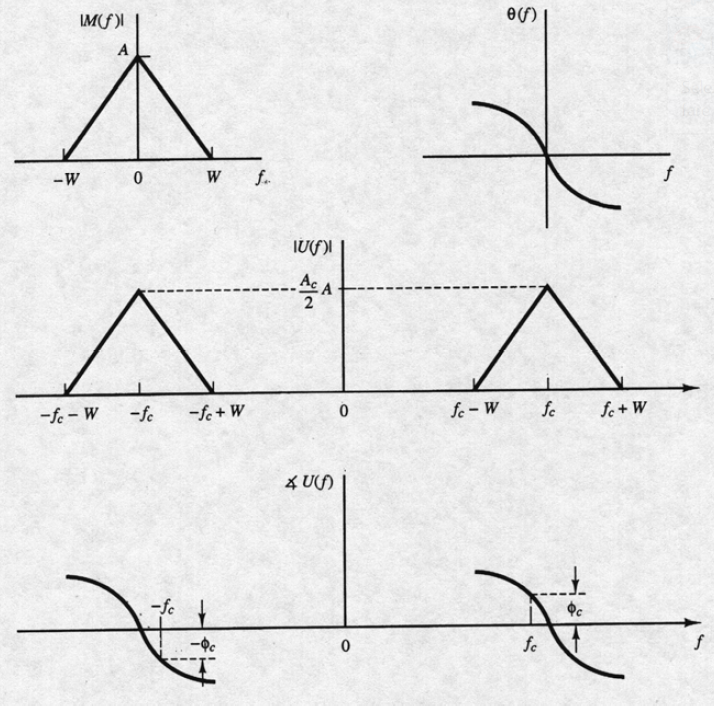
\includegraphics[scale = 1]{Segnale modulato e modulante in AM.PNG}
\end{figure} 

Questa figura mette in evidenzia tutte le caratteristiche peculiari della modulazione DSB-SC. \newline 

La modulazione trasla lo spettro del segnale di $\abs{M(f)}$ da $[-W, +W]$ a $\abs{U(f)}$ in $[-f_c - W, -f_c +W]$ e $[f_c - W, f_c +W]$. \newline 

Il modulo di $\abs{M(f)}$ in $\abs{U(f)}$ resta inalterato (a meno di un fattore moltiplicativo che è $\frac{A_c}{2}$). \newline 

L'unico parametro che cambia è quello della fase che passa da $\theta(f) = 0$ in f a $-\theta_c$ a $-f_c$ e $\theta_c$ a $f_c$. \newline 

In altre parole, la fase iniziale viene incrementata di $\theta_c$ nelle frequenze positive e viene ridotta di $\theta_c$ per quanto riguarda le frequenze negative. \newline 

A meno di questo sfasamento (che peraltro è nullo quando $\theta_c = 0$), 
lo spettro del segnale non viene modificato dalla modulazione. \newline 

Per questo motivo, la modulazione DSB-SC, e più in generale la modulazione in ampiezza, 
viene classificata come "lineare" anche se non è una modulazione svolta con componenti lineari. \newline 

Un sistema lineare, può eliminare (cioè si comporta da filtro) o equalizzare (cioè svolge un equalizzatore di ampiezza o di fase) totalmente o in parte le frequenze che gli si presentano in ingresso, 
ma non ne potrà mai introdurre di nuove. \newline 

Dalla figura degli spettri del segnale modulato rispetto al segnale modulante, 
$M(f)$ occupa una banda $[-W, +W]$, invece $U(F)$ occupa $[-f_c - W, -f_c +W]$ e $[f_c - W, f_c +W]$, 
che è il doppio della banda occupata da M(f). \newline 

Prende il nome di banda laterale superiore di U(f) (o come è stato definito a lezione Banda Laterale Superiore BLSup) 
la parte dello spettro per $\abs{f} > f_c$. \newline 

Prende il nome di banda laterale inferiore di U(f) (o come è stato definito a lezione Banda Laterale Inferiore BLInf) 
la parte dello spettro per $\abs{f} < f_c$. \newline 

Il seguente schema ci può far capire meglio la differenza tra banda laterale superiore e banda laterale inferiore: 

\begin{figure}[h]
    \centering
    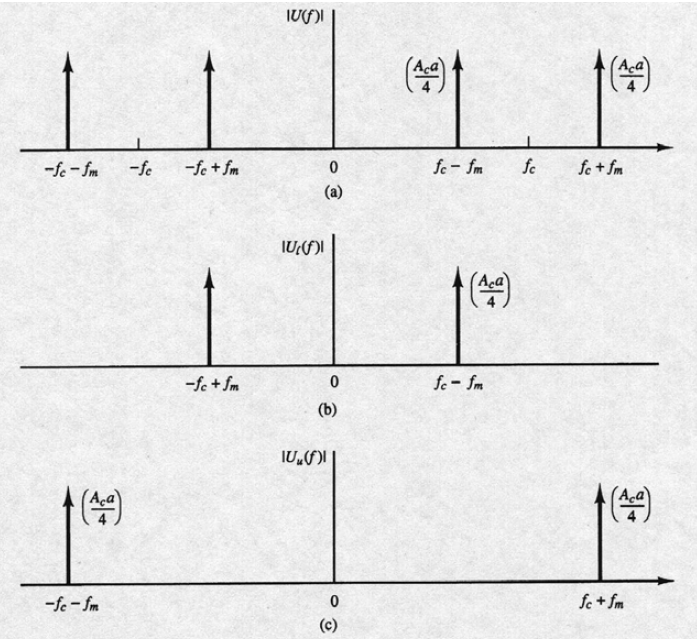
\includegraphics[scale = 1]{Bande laterali.PNG}
\end{figure} 

Se la modulante è sinusoidale, grazie alle proprietà di Fourier, avremo come segnale modulato una serie di righe nello spettro in frequenza (come si vede in figura da $\abs{U(f)}$). \newline 

$\abs{U_u (f)}$ è lo spettro della banda superiore (u dall'inglese si intende upper, superiore in italiano), 
$\abs{U_l (f)}$ è lo spettro della banda inferiore (l dall'inglese si intende lower, inferiore in italiano) 

Quindi, come si vede dalla figura, in $\abs{U_u (f)}$ ci sono solo le frequenze a $[-f_c + f_m]$ e $[f_c - f_m]$, 
in $\abs{U_l (f)}$ ci sono solo le frequenze a $[-f_c - f_m]$ e $[f_c + f_m]$. \newline 

Grazie al concetto dei processi stocastici, in particolare della teoria dei processi ciclo-stazionari, i segnali determinati e le loro proprietà si estendono anche ai segnali di spettro di potenza, 
cioè quelli che abbiamo visto in figura. \newline 

\begin{tcolorbox}
    
    Da \url{https://github.com/ciccio25/appunti-teoria-dei-segnali/blob/main/Appunti%20Teoria%20dei%20segnali.pdf} \\
    Capitolo 13 Processi stocastici | pag 151 - 160 \newline

\end{tcolorbox}

\newpage 

\subsubsection{Demodulazione per la DSB-SC}
\footnote{Slide del prof | Modulazioni analogiche | pag 6 - 8\\  
Appunti di Damiano| pag 6 - 8\\
Appunti | Modulazioni analogiche | pag 6 - 8 \\
Appunti | 2025-03-03 | pag 3 - 11
} 

Un ultimo aspetto riguarda la demodulazione, cioè la capacità di riottenere il segnale modulante a partire dal segnale modulato. \newline 

In un sistema di comunicazioni, la demodulazione avviene al lato ricevente quando si deve recuperare l'informazione m(t) per renderla utilizzabile dal destinatario. \newline 

Si pensi ad un segnale telefonico: la voce umana sta nella banda da 300 Hz a 3400 Hz. \newline 

Nella trasmissione sul canale, ad esempio il cavo di rame, il segnale voce viene modulato ad alta frequenza 
in modo da essere trasportato nella rete di telecomunicazioni, e alla fine viene ricevuto dal destinatario che riporta il segnale modulato in alta frequenza alla frequenza originale, 
così da poter ascoltare la voce del mittente. \newline 

In assenza di rumore, distorsione o altre cause di disturbo, 
il segnale ricevuto r(t) coincide con m(t): 
il modo concettuale per riottenere il segnale m(t) non è quello di dividere per la portante, 
bensì moltiplicare r(t) per un segnale sinusoidale. \newline 

Il segnale sinusoidale sarà proprio il segnale di portante, che è sta generata localmente dal ricevitore, 
con la stessa frequenza e con la stessa fase della portante ricevuta. \newline 

In formule, se si è ricevuto r(t) e grazie alle proprietà trigonometriche: 

{
    \Large 
    \begin{equation}
        \begin{split}
        r(t) \cdot \cos(2 \pi f_c t + \phi_c) 
        &=
        A_c \cos^{2}(2 \pi f_c t + \phi_c)
        \\
        &=
        A_c m(t) \cdot \frac{1 + \cos[2\cdot (2 \pi f_c t + \phi_c)]}{2} 
        \\
        &=
        \frac{1}{2} A_c m(t)
        +
        \frac{1}{2} A_c m(t)
        \cos[2\cdot (2 \pi f_c t + \phi_c)]
        \\
        &=
        \frac{1}{2} A_c m(t)
        +
        \frac{1}{2} A_c m(t)
        \cos(4 \pi f_c t + 2 \phi_c)
    \end{split}
    \end{equation}
}

\begin{tcolorbox}
    Ripasso delle formule trigonometriche che non fa mai male: \\
    \url{https://www.youmath.it/formulari/65-formulari-di-trigonometria-logaritmi-esponenziali/159-identita-trigonometriche-formule-di-prostaferesi-formule-di-werner.html} \newline 

    In questo corso le utilizzeremo spesso, quindi può essere comodo averle sempre sotto mano
\end{tcolorbox}

Osservando la formula appena scritta, possiamo fare le seguenti considerazioni: 

\begin{itemize}
    \item Aggiungendo un filtro passa basso con frequenza di taglio a $2 \pi f_c$, possiamo togliere tutta la componente in alta frequenza 
    \item $\frac{1}{2} A_c$ è solo un fattore moltiplicativo
\end{itemize}

Con queste osservazioni, possiamo semplificare l'equazione del demodulatore come: 

{
    \Large 
    \begin{equation}
        \begin{split}
        r(t) \cdot \cos(2 \pi f_c t + \phi_c) 
        &=
        \frac{1}{2} A_c m(t)
        +
        \frac{1}{2} A_c m(t)
        \cos(4 \pi f_c t + 2 \phi_c)  
        \\
        &\downarrow
        \\
        r(t) \cdot \cos(2 \pi f_c t + \phi_c)
        &= 
        \frac{1}{2} A_c m(t)
        \end{split}
    \end{equation}
}

Cioè il segnale ricevuto e de-modulato è proprio il segnale originale in banda base, a meno del fattore moltiplicativo $\frac{1}{2} A_c$. \newline 

Possiamo schematizzare il demodulatore con la seguente figura: 

\begin{figure}[h]
    \centering
    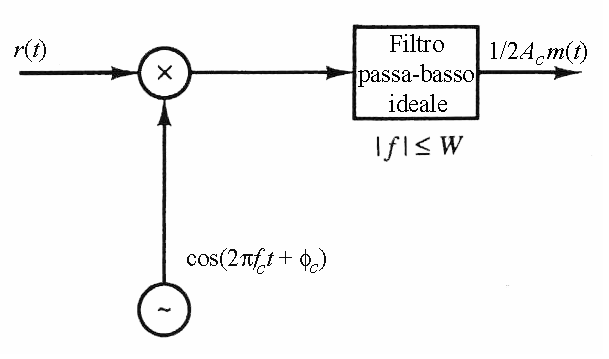
\includegraphics[scale = 1]{Schema architettura di un demodulatore.png}
\end{figure} 

Se invece consideriamo una differenza di fase tra la portante ricevuta e la portante generata localmente, 
avremo la seguente equazione: 

{
    \Large 
    \begin{equation}
            r(t) \cos(2 \pi f_c t + \phi)
            = 
            \frac{1}{2} A_c m(t) \cos(\phi_c - \phi)
            + 
            \frac{1}{2} A_c m(t) \cos(4 \pi f_c t + \phi_c - \phi)
    \end{equation}
}

A valle del filtro passa-basso del demodulatore, e per le considerazioni svolte precedentemente, avremo il segnale di uscita $y_l (t)$:

{
    \Large 
    \begin{equation}
        \begin{split}
            r(t) \cos(2 \pi f_c t + \phi)
            &= 
            \frac{1}{2} A_c m(t) \cos(\phi_c - \phi)
            + 
            \frac{1}{2} A_c m(t) \cos(4 \pi f_c t + \phi_c - \phi)
            \\
            &\downarrow
            \\
            y_l (t)
            &= 
            \frac{1}{2} A_c m(t) \cos(\phi_c - \phi)
        \end{split}
    \end{equation}
}

Questa ultima espressione di $y_l (t)$ mette in evidenzia che, rispetto al caso ideale: 

{
    \Large 
    \begin{equation}
        y_l^{'} (t) = \frac{1}{2} A_c m(t)
    \end{equation}
}

il segnale utile in uscita è ridotto del fattore $\cos(\theta_c - \theta)$. \newline 

Se: 

{
    \Large 
    \begin{equation}
        \theta_c - \theta = 90 ^{\circ}
    \end{equation}
}

$y_l (t)$ diventa: 

{
    \Large 
    \begin{equation}
       \begin{split}
        y_l (t)
            &= 
            \frac{1}{2} A_c m(t) \cos(\phi_c - c)
            \\
            &\downarrow
            \\
            y_l (t)
            &= 
            \frac{1}{2} A_c m(t) \cos(90 ^{\circ})
            \\
            &= 
            \frac{1}{2} A_c m(t) \cdot 0 
            \\
            &= 
            0
       \end{split} 
    \end{equation}
}

cioè $y_l (t)$ si annulla. \newline 

In caso di un segnale utile sovrapposto ad un contributo di rumore (ad esempio il rumore termico), 
la rivelazione imperfetta riduce la potenza del segnale utile, rendendo quest'ultimo più vulnerabile agli effetti del rumore. \newline 

Il demodulatore raffigurato precedentemente è detto anche ricevitore sincrono (o coerente). \newline 

Viene definito ricevitore coerente perché, per ricavare il segnale modulante, 
si moltiplica il segnale modulato per un coseno. \newline  

Il problema della ricostruzione della fase $\theta_c$ della portante è uno dei problemi di maggior importanza nell'ambito della ricezione sincrona e viene tipicamente risolto con i PLL (Phase-Locked Loop). \newline 

In alternativa, la demodulazione può essere semplificata sovrapponendo alla trasmissione del segnale DSB-SC la trasmissione di un residuo di portante, 
utilizzando il seguente schema: 

\begin{figure}[h]
    \centering
    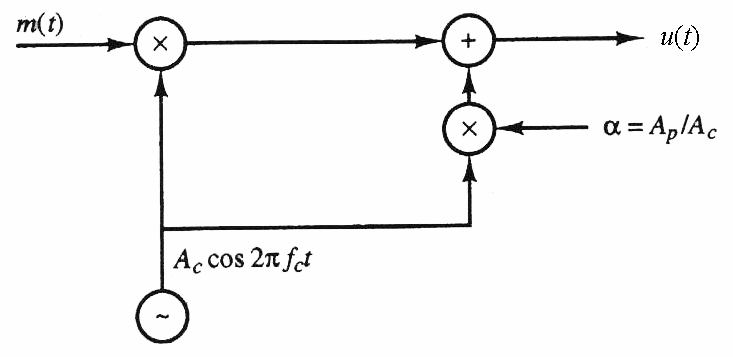
\includegraphics[scale = 1]{Modulazione DSB-SC con resudio di portante.png}
\end{figure} 

Rispetto al caso precedente, u(t) sarà: 

{
    \Large 
    \begin{equation}
        u (t)
        = 
        \left[A_c m(t) + \frac{A_p}{A_c} \right] \cdot \cos(2 \pi f_c t)
    \end{equation}
}

dove $A_p$ viene definito come residuo di portante, la cui ampiezza è una frazione di $\alpha$ di $A_c$: 
$A_c$ viene definito come tono pilota. \newline 

\newpage 

In frequenza avremo: 

\begin{figure}[h]
    \centering
    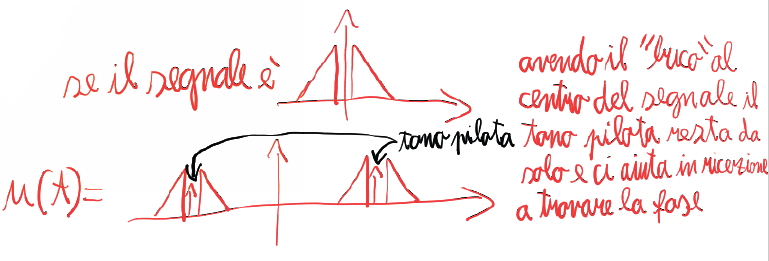
\includegraphics[scale = 1]{Aggiunta del tono pilota DSB-SC.PNG}
\end{figure} 

Con questo schema non vi è necessità di generare localmente la portante al ricevitore, 
ma il prezzo che si paga è in termini di potenza trasmessa addizionale e di intervallo di frequenza non utilizzabile 
perché necessario alla trasmissione della portante. \newline 

In questo senso, rispetto al caso senza tono pilota, lo schema DSB-SC costituisce una soluzione "ibrida", 
che permette di avere un demodulatore più semplice ed a costo economico ridotto, ma sprecando nettamente più energia in trasmissione. \newline 

\newpage 

\subsection{Modulazione di ampiezza convenzionale - AM}
\footnote{Slide del prof | Modulazioni analogiche | pag 8 - 11\\  
Appunti di Damiano| pag 8 - 11\\
Appunti | Modulazioni analogiche | pag 8 - 11\\
Appunti | 2025-03-03 | pag 11 - 13
}

Nella sezione precedente, cioè riguardo alla DSB-SC, abbiamo discusso e analizzato una DSB-SC con una portante quando si va in trasmissione per semplificare il ricevitore: 
questo caso particolare è proprio la tecnica AM (Amplitude Modulation) convenzionale della modulazione DSB-SC. \newline 

Riportando lo schema del modulatore AM: 

\begin{figure}[h]
    \centering
    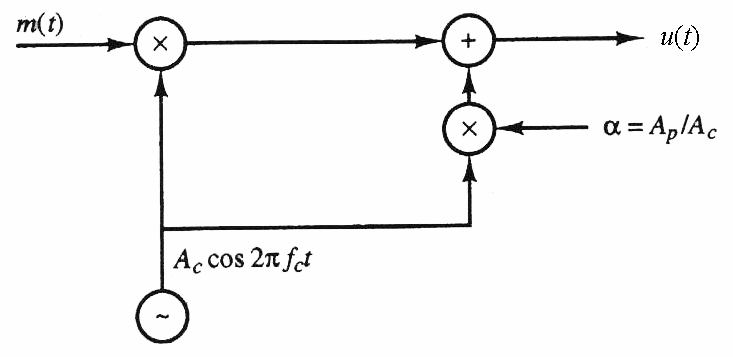
\includegraphics[scale = 1]{Modulazione DSB-SC con resudio di portante.png}
\end{figure} 

il segnale modulato in uscita u(t) sarà: 

{
    \Large 
    \begin{equation}
        u (t)
        = 
        A_c 
        [1 + \alpha \cdot m_n (t)] 
        \cos(2 \pi f_c t + \phi_c)
    \end{equation}
}

dove: 

{
    \Large 
    \begin{equation}
        \begin{cases}
            m_n(t) = \frac{m(t)}{\max \abs{m(t)}}
            \\
            0 < \alpha \le 1
        \end{cases}    
    \end{equation}
}

$m_n (t)$ è definito come "segnale modulante normalizzato", 
invece $\alpha$ è definito come "indice di modulazione di ampiezza". \newline 

Grazie alle definizioni di $m_n (t)$ e $\alpha$, possiamo dire che u(t) non diventa mai negativa nel tempo. \newline 

Considerando il caso particolare in cui:

{
    \Large 
    \begin{equation}
        \begin{cases}
            m_n(t_0) = - 1 
            \\
            \alpha = 1
        \end{cases}
    \end{equation}
}

\newpage 

l'andamento del segnale modulato u(t) è il seguente: 

\begin{figure}[h]
    \centering
    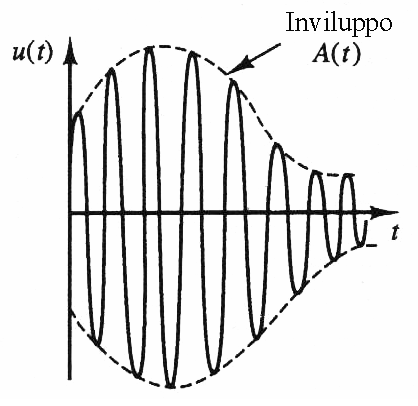
\includegraphics[scale = 1]{Segnale modulato AM con alpha a 1.png}
\end{figure} 

e confrontando il segnale modulato in AM con quello a DSB-SC: 

\begin{figure}[h]
    \centering
    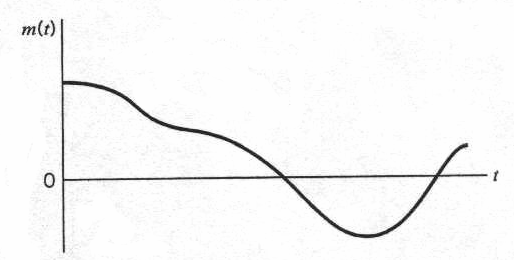
\includegraphics[scale = 0.8]{Segnale modulante.png}
    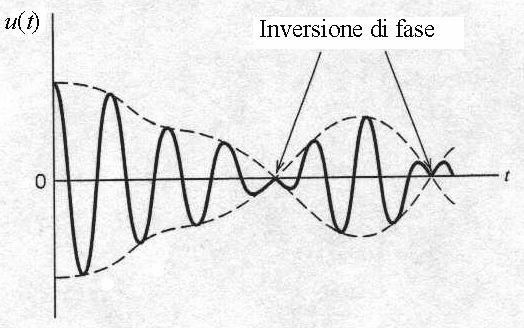
\includegraphics[scale = 0.8]{Segnale modulato in AM.png}
\end{figure}

notiamo che in AM, l'inviluppo mantiene l'andamento del segnale modulante (cioè quello tratteggiato in figura): 
è proprio per questa caratteristica che la demodulazione del segnale AM convenzionale può essere particolarmente semplice. \newline 

Inoltre, nei passaggi sullo zero, in AM non ci sono inversioni della fase. \newline 

Per inviluppo si intende che la sequenza dei massimi tra segnale modulato e modulante è la stessa. \newline 

La trasformata di Fourier di un segnale in AM convenzionale diventa: 

{
    \Large 
    \begin{equation}
        \begin{split}
        u (t)
        &= 
        A_c 
        [1 + \alpha \cdot m_n (t)] 
        \cos(2 \pi f_c t + \phi_c)
        \\
        &\quad
        \\
        &\downarrow
        \\
        &\quad
        \\
        U(f)
        &= 
        \frac{A_c}{2}
        \left[
            e^{\jmath \phi_c} a M_n (f - f_c)
            +
            e^{\jmath \phi_c} \delta (f - f_c)
            +
            e^{-\jmath \phi_c} a M_n (f + f_c)
            +
            e^{-\jmath \phi_c} \delta (f + f_c)
        \right]
    \end{split}
    \end{equation}
}

dove $M_n (f)$ è la trasformata di Fourier del segnale modulante normalizzato. \newline 

\newpage 

Un esempio di andamento di U(f), nel caso di modulante sinusoidale, è mostrato nella seguente figura: 

\begin{figure}[h]
    \centering
    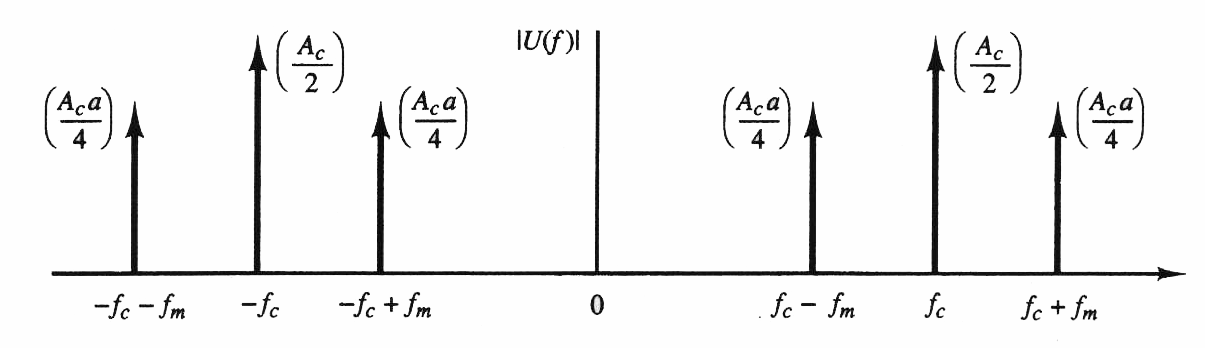
\includegraphics[scale = 0.6]{Segnale modulato in AM in frequenza.png}
\end{figure} 

Rispetto allo spettro in frequenza di un segnale modulato in DSB-SC: 

\begin{figure}[h]
    \centering
    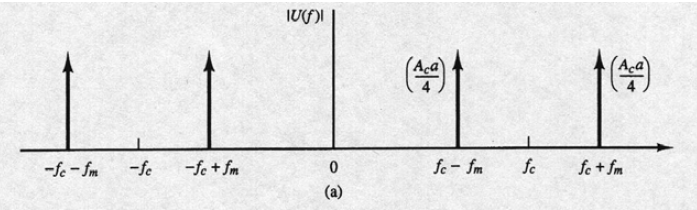
\includegraphics[scale = 1]{Segnale modulato in DSB-SC.PNG}
\end{figure} 

notiamo che, in AM convenzionale, è presente la portante a $\abs{f_c}$. \newline

Inoltre, si nota dalla figura, che, se ci troviamo nel caso di $\alpha = 1$, 
l'ampiezza della portante resta doppia di quella di ciascuno dei segnali assegnati alle bande laterali (in questo caso particolare, a loro volta sinusoidali). \newline 

Di conseguenza, anche nel caso limite di modulazione al 100 \%, cioè $\alpha = 1$, 
i $\frac{2}{3}$ della potenza complessiva del segnale modulato sono associati alla portante 
e solo la frazione rimanente, cioè $\frac{1}{3}$ è associata alla bande laterali. \newline 

Con valori di $\alpha < 1$, questo "squilibrio" si enfatizza, specialmente nei casi in cui $\alpha < \frac{1}{2}$, 
che sono la grande maggioranza dei segnali di interesse. \newline 

Il fatto di usare la maggior parte dell'energia di un segnale modulato per la portante è molto inefficiente dal punto di vista energetico, 
ma è molto utile per realizzare un circuito di demodulazione molto semplice. \newline 

Essendo l'informazione contenuta nell'inviluppo del segnale, 
è sufficiente ricostruire al ricevitore proprio l'inviluppo. \newline 

Quindi non è necessario un ricevitore coerente come nella DSB-SC (anche se tecnicamente lo si potrebbe utilizzare), 
ma possiamo utilizzare questo semplice circuito del demodulatore a inviluppo: 

\begin{figure}[h]
    \centering
    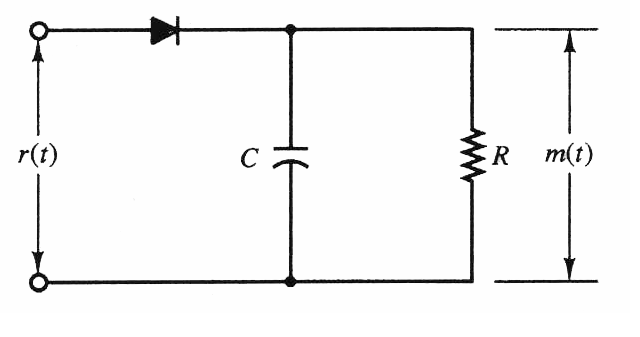
\includegraphics[scale = 1]{Demodulatore di inviluppo.png}
\end{figure} 

Questo demodulatore si definisce non coerente perché non si moltiplica r(t) per un coseno. \newline 

I componenti di questo demodulatore sono i seguenti: 

\begin{itemize}
    \item diodo, che è un componente non lineare che elimina le componenti r(t) quando quest'ultima diventa negativa 
    \item una capacità C 
    \item un resistore R
\end{itemize}

Attraverso una scelta adeguata dei componenti R-C (che realizzano un filtraggio passa-basso), 
si ottiene un andamento del segnale come la seguente figura: 

\begin{figure}[h]
    \centering
    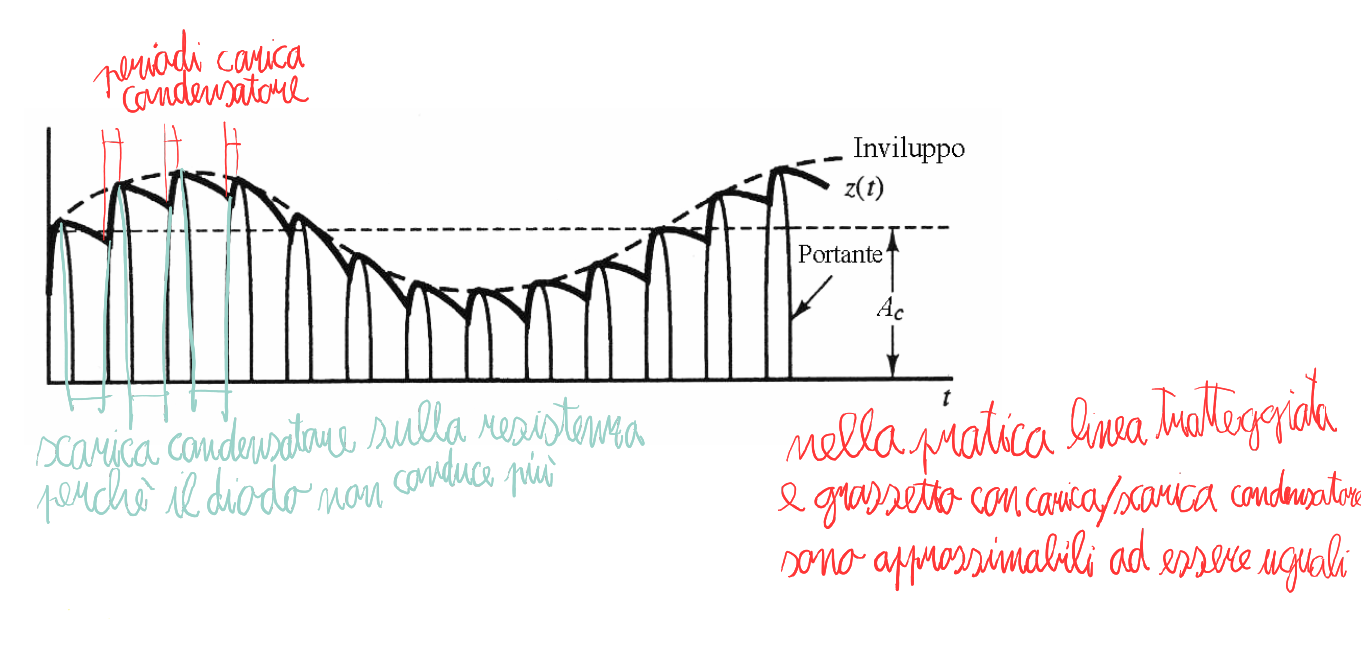
\includegraphics[scale = 0.65]{Segnale demodulato in AM con demodulatore a inviluppo.PNG}
\end{figure} 

La scelta di semplificare il ricevitore è decisiva in tutte quelle applicazioni in cui il numero dei trasmettitori è ridotto, 
mentre è elevato il numero dei ricevitori. \newline 

Per questo motivo l'utilizzo della AM convenzionale, o altre tecniche simili,
ha costituito la soluzione privilegiata (negli anni precedenti prima dell'avvento del digitale e dei componenti a basso costo)
per i servizi commerciali di tipo diffusivo come radio e televisione. \newline 

\newpage 

\subsection{Banda Laterale Unica (SSB)}
\footnote{Slide del prof | Modulazioni analogiche | pag 11 - 13\\  
Appunti di Damiano| pag 11 - 13\\
Appunti | Modulazioni analogiche | pag 11 - 13\\
Appunti | 2025-03-03 | pag 13
} 

L'obbiettivo della modulazione di ampiezza a banda laterale unica (acronimo italiano BLU o, in inglese SSB Single Side Band) 
è quello di migliorare l'efficienza spettrale. \newline 

Nelle tecniche precedenti trattate, cioè DSB-SC e AM convenzionale, 
la banda occupata dal segnale modulato era doppia rispetto a quella del segnale modulante. \newline 

Osservando alla forma dello spettro del segnale modulato, ad esempio quello in DSB-SC, e al modo in cui è stato ottenuto per traslazione dello spettro della banda base: 

\begin{figure}[h]
    \centering
    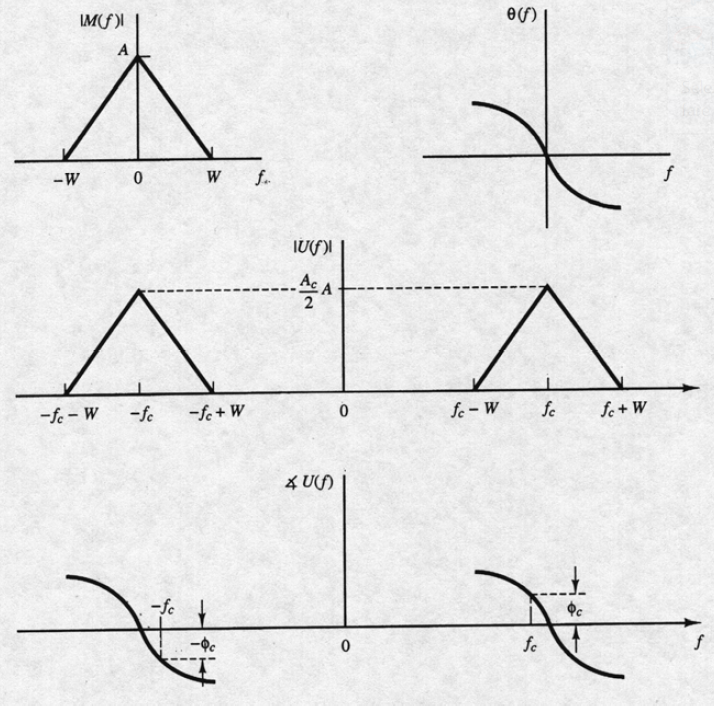
\includegraphics[scale = 0.7]{Segnale modulato e modulante in AM.PNG}
\end{figure} 

ci si convince facilmente che la ricostruzione del segnale è possibile anche conoscendo soltanto una delle due bande laterali. \newline 

L'andamento temporale del segnale SSB è del tipo: 

{
    \Large 
    \begin{equation}
        u(t)
        =
        A_c m(t) \cos(2 \pi f_c t)
        \mp
        A_c \tilde{m}(t) \sin(2 \pi f_c t)
    \end{equation}
}

dove $\tilde{m}(t)$ è la trasformata di Hilbert del segnale modulante. \newline 

\begin{tcolorbox}
    Come al solito, un altro argomento che abbiamo incontrato e studiato al precedente corso. \newline 

    Da \url{https://github.com/ciccio25/appunti-teoria-dei-segnali/blob/main/Appunti%20Teoria%20dei%20segnali.pdf} \\
    Capitolo 8 Trasformata di Hilbert | pag 83 - 85 \newline

\end{tcolorbox}

Per semplicità, si è trascurata la fase iniziale della portante $\phi_c$. \newline 

Nella formula è presente un segno $\mp$ perché si utilizza uno dei due casi: 

\begin{itemize}
    \item il segno negativo - se si è deciso di trasmettere la banda laterale superiore 
    \item il segno positivo + se si è deciso di trasmettere la banda laterale inferiore 
\end{itemize}

\newpage

Dalla formula di u(t) possiamo ricavare uno schema a blocchi del modulatore, che è il seguente: 

\begin{figure}[h]
    \centering
    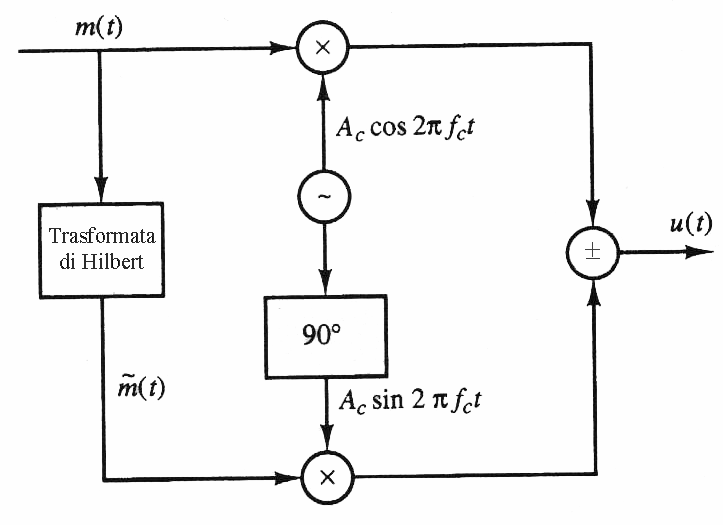
\includegraphics[scale = 0.7]{Modulazioone segnale SSB.png}
\end{figure}

Dalle proprietà della trasformata di Hilbert, ricordiamo che m(t) 
non deve avere un contenuto significativo alle basse frequenze, perché altrimenti si perderà informazione. \newline 

In alternativa, la stessa modulazione SSB può essere applicata con il seguente schema: 

\begin{figure}[h]
    \centering
    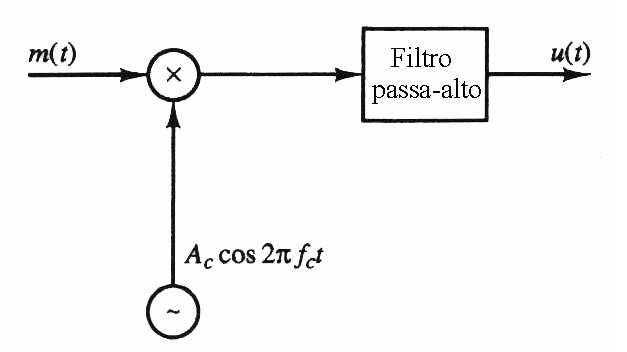
\includegraphics[scale = 0.7]{Modulazioone segnale SSB con filtro passa alto e DSB-SC.png}
\end{figure}

dove è presente un filtro passa-alto, con frequenza di taglio in prossimità della frequenza di portante $f_c$, 
del segnale m(t) modulato in DSB-SC.\newline 

\newpage 

Un esempio di spettro di segnale SSB, nel caso di segnale modulante stocastico è riportato nella seguente figura: 

\begin{figure}[h]
    \centering
    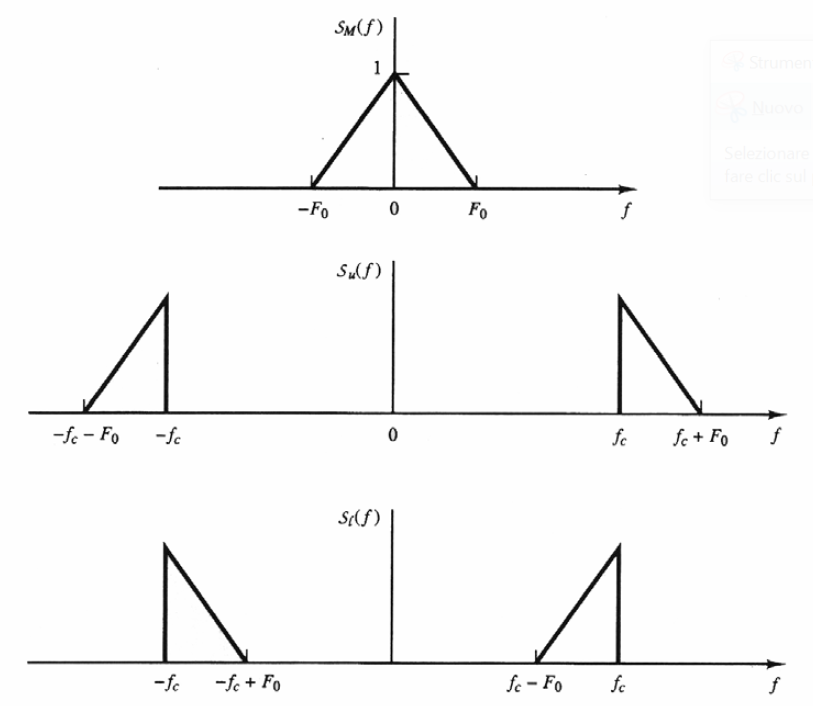
\includegraphics[scale = 0.7]{Spettri di potenza di un segnale in BB e SSB.PNG}
\end{figure}

dove: 

\begin{itemize}
    \item $S_M (f)$ è il segnale modulante in Banda Base 
    \item $S_u (f)$ è il segnale modulato in SSB con banda laterale superiore 
    \item $S_l (f)$ è il segnale modulato in SSB con banda laterale inferiore
\end{itemize}

Sapendo che il segnale modulante $S_M (f)$ si estende in banda da $[- F_0, +F_0]$, 
trasmettendo solo in banda superiore o solo in basa superiore, si occupa la metà della banda rispetto alla DSB-SC e la AM-convenzionale, 
mantenendo la stessa qualità. \newline 

O se si applica il filtraggio passa-alto dalla modulazione della DSB-SC o si utilizza il metodo con la trasformata di Hilbert, 
la SSB è assente di componenti significativi intorno alla frequenza d'origine. \newline 

Se infatti idealmente il filtraggio di Hilbert o quello passa-banda può avvenire con transizione brusca (o a frequenza nulla per la trasformata di Hilbert o a $f_c$ per il filtro passa-alto), 
come si può visualizzare nel seguente andamento del filtro di Hilbert: 

\begin{figure}[h]
    \centering
    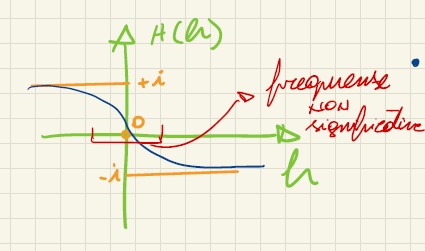
\includegraphics[scale = 0.5]{Considerazioni filtro di Hilbert in frequenza.PNG}
\end{figure} 

nella pratica un filtro reale presenterà una regione di transizione che, inevitabilmente, distorcerà, se presenti, le componenti armoniche al suo interno. \newline 

Questo giustifica il fatto che la modulazione SSB può essere utilizzata per il segnale telefonico, perché lo spettro significativo del parlato inizia dai 300 Hz in su, 
mentre non si può applicare al segnale televisivo, in cui il contenuto armonico include anche le bassissime frequenze 
(in rapporto alla larghezza di banda del segnale televisivo). \newline 

\newpage 

\subsubsection{Demodulazione SSB}
\footnote{Slide del prof | Modulazioni analogiche | pag 13 \\  
Appunti di Damiano| pag 13 \\
Appunti | Modulazioni analogiche | pag 13 \\
Appunti | 2025-03-03 | pag 13 - 14
} 

La demodulazione del segnale modulato in SSB: 

{
    \Large 
    \begin{equation}
        u(t)
        =
        A_c m(t) \cos(2 \pi f_c t)
        \mp
        A_c \tilde{m}(t) \sin(2 \pi f_c t)
    \end{equation}
}

deve, per forza, necessariamente avvenire con tecnica coerente. \newline 

\begin{tcolorbox}
    Come dice il Darione: \newline

    
\includegraphics[scale = 0.3]{dario-moccia-per-forza.jpg }
\end{tcolorbox}

Si pongono le stesse criticità già evidenziate per la tecnica DSB-SC, 
ma aggravate dal fatto che l'eventuale non coincidenza tra la fase $\phi_c$ della portante trasmessa e quella $\phi$, 
della portante generata localmente, si  traduce qui non una semplice attenuazione (come per la DSB-SC), 
ma in una distorsione del segnale demodulato. \newline 

Per esempio, posto per semplicità $\phi_c = 0$ e supponendo di aver trasmesso la banda laterale superiore, ove sia $\phi \neq 0$, 
utilizzando lo stesso schema circuitale della DSB-SC, cioè un filtro coerente: 

\begin{figure}[h]
    \centering
    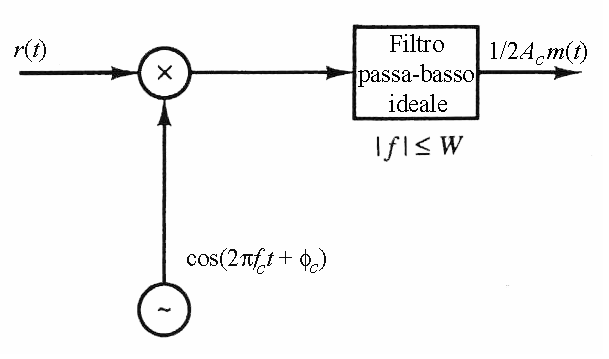
\includegraphics[scale = 1]{Schema architettura di un demodulatore.png}
\end{figure} 

dove avevamo nel caso DSB-SC: 

{
    \Large 
    \begin{equation}
        y_l (t)
        = 
        \frac{1}{2} A_c m(t) \cos(\phi_c - c)
    \end{equation}
}   

nel caso SSB in banda laterale superiore con $\phi_c = 0$, 
avremo che: 

{
    \Large 
    \begin{equation}
        \begin{split}
        u(t)
        &=
        A_c m(t) \cos(2 \pi f_c t)
        -
        A_c \tilde{m}(t) \sin(2 \pi f_c t) 
        \\
        &\downarrow
        \\
        y_l (t)
        &=
        \frac{1}{2} A_c m(t) \cos(\phi)
        + 
        \frac{1}{2} A_c \tilde{m}(t) \sin(\phi)
        \end{split}
    \end{equation}
}

Dalla formula di $y_l (t)$ notiamo che il segnale utile $\frac{1}{2} A_c m(t) \cos(\phi)$ 
è sovrapposto alla sua trasformata di Hilbert, che è ovviamente diversa dal segnale originale. \newline 

Ecco perché è importante realizzare un controllo molto accurato della fase $\phi$ al ricevitore (ad esempio impiegando i PLL), 
in modo da evitare che il problema evidenziato si presenti. \newline 

Per problema evidenziato della fase $\phi$ si intende che, nel caso peggiore in cui: 

{
    \Large 
    \begin{equation}
        \phi = 0^{\circ}
    \end{equation}
}

allora: 

{
    \Large 
    \begin{equation}
        \begin{split}
        y_l (t)
        &=
        \frac{1}{2} A_c m(t) \cos(\phi)
        + 
        \frac{1}{2} A_c \tilde{m}(t) \sin(\phi)
        \\
        &\downarrow
        \\
        y_l (t)
        &=
        \frac{1}{2} A_c m(t) \cos(0^{\circ})
        + 
        \frac{1}{2} A_c \tilde{m}(t) \sin(0^{\circ})
        \\
        &= 
        0
        +
        \frac{1}{2} A_c \tilde{m}(t)
        \\
        &= 
        \frac{1}{2} A_c \tilde{m}(t)
        \end{split}
    \end{equation}
}

cioè è presente solo la trasformata di Hilbert di m(t). \newline 

In modo da evitare questo problema, come ribadito nella DSB-SC, si può trasmettere un tono pilota a $f_c$, 
sprecando sulla potenza e sulla efficienza notevole della modulazione SSB. \newline 

\newpage 

\subsubsection{Modulazione di ampiezza con portanti in quadratura}
\footnote{Slide del prof | Modulazioni analogiche | pag 13 - 14\\  
Appunti di Damiano| pag 13 - 14\\
Appunti | Modulazioni analogiche | pag 13 - 14\\
Appunti | 2025-03-03 | pag 13 - 15
} 

A chiusura di questo sezione, vogliamo evidenziare che la medesima efficienza spettrale del segnale SSB 
può essere conseguita utilizzando due portanti in quadratura, alla stessa frequenza, 
a ciascuna delle quali sia associato un diverso segnale modulante. \newline 

La funzione del tempo che ne risulta può essere scritta come: 

{
    \Large 
    \begin{equation}
        u (t)
        = 
        A_c m_1 (t) \cos(2 \pi f_c t)
        + 
        A_c m_2 (t) \cos(2 \pi f_c t)
    \end{equation}
}

La seguente figura mostra a sinistra la generazione del segnale al lato trasmettitore, 
mentre a destra della figura si recupera $m_1 (t)$ e $m_2 (t)$ al lato ricevitore: 

\begin{figure}[h]
    \centering
    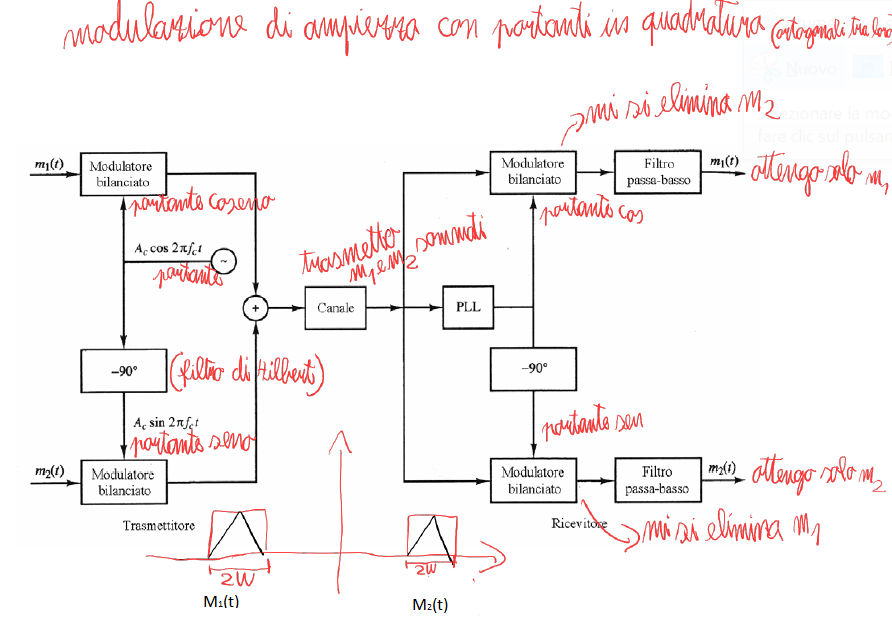
\includegraphics[scale = 1]{Schema con note di modulatore e demodulatore in quadratura.png}
\end{figure} 

Questo tipo di schema ci permette di dire che è possibile realizzare delle modulazioni DSB-SC che in ricezione è possibile separare, 
grazie alla ortogonalità delle portanti. \newline 

Pertanto, in questo caso, si pongono gli stessi problemi di ricostruzione della fase, 
e se ciò non avviene a dovere, il segnale, ad esempio $m_1(t)$, 
sarà sovrapposto a un residuo dell'altro segnale $m_2 (t)$: questa sovrapposizione è definita come cross-talk. \newline 

La modulazione di ampiezza con portanti in quadratura è l'archetipo di una delle modulazioni più importanti: 
la cosiddetta QAM Quadrature Amplitude Modulation, che avremo di approfondire nell'ambito delle modulazioni digitali. \newline 

\newpage 

\subsection{Banda laterale ridotta - VSB}
\footnote{Slide del prof | Modulazioni analogiche | pag 14 - 15\\  
Appunti di Damiano| pag 14 - 15\\
Appunti | Modulazioni analogiche | pag 14 - 15\\
Appunti | 2025-03-04 | pag 2 - 4\\ 
Appunti | 2025-07-08 Ricevimento | pag 10
} 

Per i segnali le cui caratteristiche spettrali non consentono l'utilizzo della modulazione SSB, 
si può migliorare l'efficienza spettrale utilizzando la modulazione di ampiezza a banda laterale ridotta 
(BLR in italiano, o in inglese VSB Vestigal Side Band). \newline 

\begin{tcolorbox}
Con la frase "i segnali le cui caratteristiche spettrali non consentono l'utilizzo della modulazione SSB" 
si intende che la SSB non è indicata per segnali che hanno una informazione significativa alle basse frequenze.  \newline

Letteralmente dall'inglese Vestigal significa residuo
\end{tcolorbox}

L'idea è quella di trasmettere un segnale che contenga una delle due bande laterali, ma anche una porzione (un vestiglio, un residuo) 
dell'altra banda laterale. \newline 

Il risultato è ottenuto con un opportuno filtraggio ad alta frequenza, come spiegato in questa figura: 

\begin{figure}[h]
    \centering
    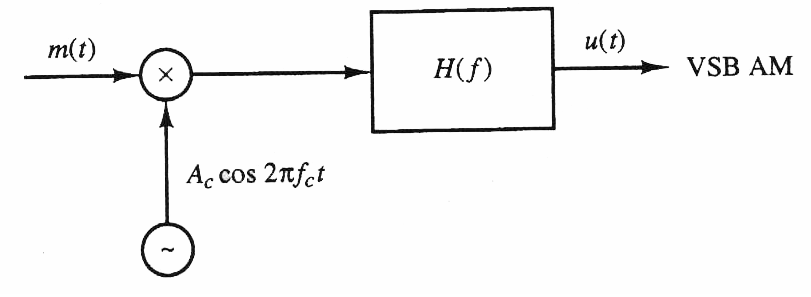
\includegraphics[scale = 0.8]{Architettura modulazione VSB.png}
\end{figure} 

Dallo schema notiamo che, nel tempo: 

{
    \Large 
    \begin{equation}
        u (t) 
        = 
        A_c m(t) \cos(2 \pi f_c t) 
        \otimes
        h(t)
    \end{equation}
}

dove: 

\begin{itemize}
    \item $A_c m(t) \cos(2 \pi f_c t)$ è il segnale modulato in DSB-SC
    \item il segno $\otimes$ indica la convoluzione 
    \item h(t) è la risposta impulsiva del filtro 
\end{itemize}

Dalle proprietà tra tempo e Fourier, sappiamo che, se facciamo una convoluzione nel tempo, avremo un prodotto in frequenza. \newline 

Quindi u(t) in Fourier diventa: 

{
    \Large 
    \begin{equation}
        \begin{split}
        u (t) 
        &= 
        A_c m(t) \cos(2 \pi f_c t) 
        \otimes
        h(t)
        \\
        U(f)
        &= 
        \frac{A_c}{2}
        \left[
            M(f - f_c) 
            +
            M(f + f_c)
        \right] 
        \cdot 
        H(f)
        \end{split}
    \end{equation}
}

Il filtro introduce massimo un'attenuazione di $\frac{1}{2}$: l'ampiezza della portante eventualmente trasmessa viene dimezzata. \newline 

Nelle applicazioni classiche della VSB (ad esempio al broadcasting televisivo), si utilizza la trasmissione della portante per semplificare il demodulatore, il quale può essere d'inviluppo. \newline 

Il filtro H(f) indicato in figura deve soddisfare la seguente condizione: 

{
    \Large 
    \begin{equation}
        H(f - f_c) 
        + 
        H(f + f_c)
        = 
        \text{ costante} 
    \end{equation}
}

Questa relazione deve essere valida per $\abs{f} \le W$. \newline 

Se questa relazione è soddisfatta, la demodulazione del segnale modulante, con banda W, avviene senza distorsione. \newline 

Come spiegato dalle seguenti figure: 

\begin{figure}[h]
    \centering
    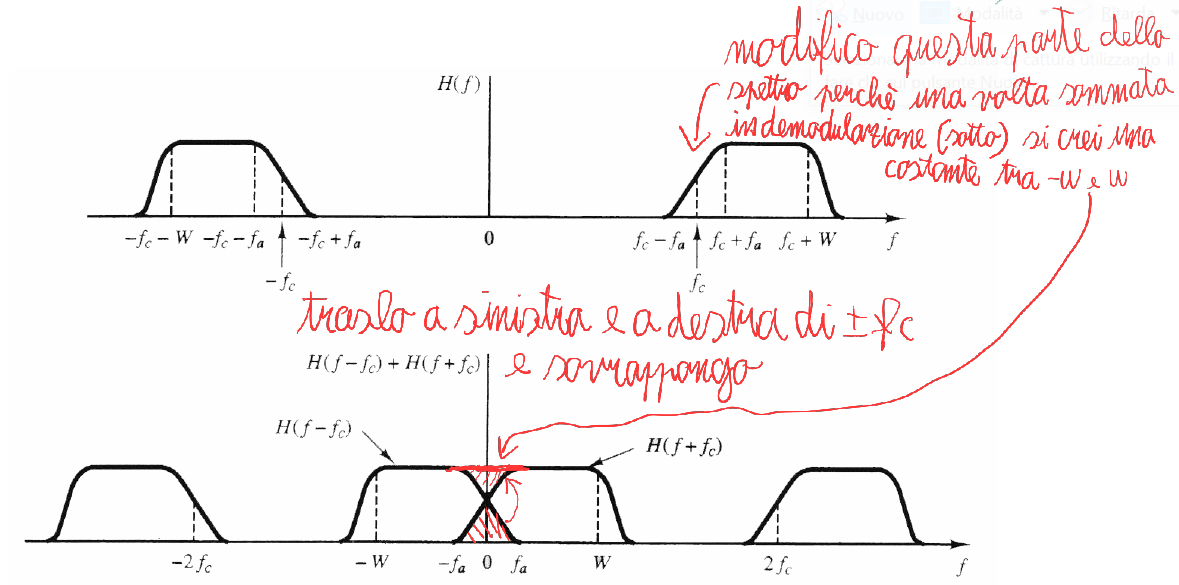
\includegraphics[scale = 0.6]{Grafici negli spettri da BB a modulato in VSB.PNG}
\end{figure} 

nella modulazione VSB, bisogna traslare una volta verso destra e una volta verso sinistra, della stessa quantità $f_c$, 
la funzione di trasferimento del filtro e di verificare che la somma delle due funzioni risultanti dalla due traslazione sia costante per $- W \le f \le +W$. \newline 

La banda occupata dal segnale VSB sarà di $W + f_a$, per cui il risparmio in banda può essere significativo. \newline 

De-modulando in modo coerente, consideriamo v(t) il segnale de-modulato nel tempo: 

{
    \Large 
    \begin{equation}
        v(t) = u(t) \cos(2 \pi f_c t)
    \end{equation}
}

In Fourier v(t) diventa: 

{
    \Large 
    \begin{equation}
        \begin{split}
           v(t) &= u^{'}(t) \cos(2 \pi f_c t)
           \\
           &\downarrow 
           \\
           V(f) &= \frac{1}{2} \left[ U(f - f_c) + U(f + f_c)\right] 
        \end{split}
    \end{equation}
}

Sostituendo il valore d U(f) a V(f), V(f) diventa: 

{
    \Large 
    \begin{equation}
        \begin{split}
             V(f) &= \frac{1}{2} \left[ U(f - f_c) + U(f + f_c)\right] 
             \\
             &\quad
             \\
             &\downarrow
             \\
             &\quad
             \\
             V(f) &= 
             \frac{A_c}{4} \left[ M(f- 2 f_c) + M(f)\right] \cdot H(f - f_c)
             +
            \frac{A_c}{4} \left[ M(f) + M(f + 2 f_c) \right] \cdot H(f + f_c)
        \end{split}
    \end{equation}
}

Riportando lo schema del demodulatore coerente: 

\begin{figure}[h]
    \centering
    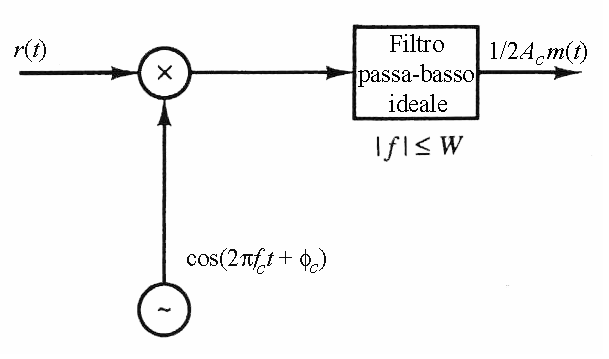
\includegraphics[scale = 1]{Schema architettura di un demodulatore.png}
\end{figure} 

i fattori $M(f- 2 f_c)$ e $M(f + 2 f_c)$ vengono eliminati, quindi V(f) si semplifica come: 

{
    \Large 
    \begin{equation}
        \begin{split}
             V(f) &= 
             \frac{A_c}{4} \left[ M(f- 2 f_c) + M(f)\right] \cdot H(f - f_c)
             +
            \frac{A_c}{4} \left[ M(f) + M(f + 2 f_c) \right] \cdot H(f + f_c)
            \\
            &\downarrow
            \\
            V(f) &= 
             \frac{A_c}{4} \left[ 0 + M(f)\right] \cdot H(f - f_c)
             +
            \frac{A_c}{4} \left[ M(f) + 0 \right] \cdot H(f + f_c)
            \\
            &= 
            \frac{A_c}{4} M(f) \left[ H(f - f_c) + H(f + f_c)\right]
        \end{split}
    \end{equation}
}

Siccome il nostro obbiettivo è recuperare M(f), cioè m(t), deve essere valida la relazione che abbiamo citato precedentemente: 

{
    \Large 
    \begin{equation}
        H(f - f_c) 
        + 
        H(f + f_c)
        = 
        \text{ costante} 
    \end{equation}
}

e per $\abs{f} \le W$. \newline 

\newpage 

\subsection{Altri schemi di modulatori di ampiezza}
\footnote{Slide del prof | Modulazioni analogiche | pag 15 - 18\\  
Appunti di Damiano| pag 15 - 18\\
Appunti | Modulazioni analogiche | pag 15 - 18\\
Appunti | 2025-03-04 | pag 5 - 7
} 

Oltre all'architetture delle modulazioni, è necessario fare qualche esempio riguardo la loro implementazione circuitale. \newline 

L'operazione di modulazione richiede, necessariamente, la presenza di componenti non lineari, 
i soli in grado di produrre le nuove frequenze richieste dalla conversione spettrale. \newline 

Un componente tipico è il diodo:  

\begin{figure}[h]
    \centering
    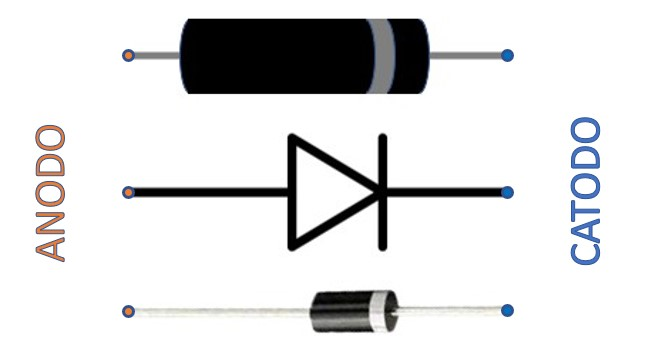
\includegraphics[scale = 0.4]{Diodo_come_funziona.jpg}
\end{figure} 

in cui la caratteristica funzione tensione-corrente ha questo tipo di andamento:

\begin{figure}[h]
    \centering
    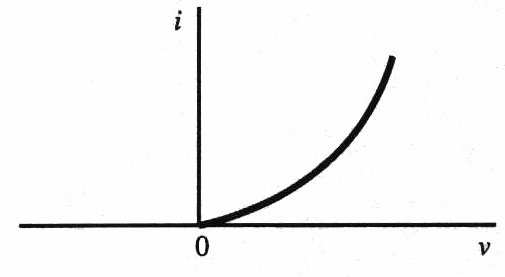
\includegraphics[scale = 0.6]{Grafico relazione tensione-corrente diodo.png}
\end{figure} 

In generale, è sufficiente la presenza di un elemento non lineare, 
la cui caratteristica ingresso-uscita presenti una componente quadratica. \newline 

Ragionando in tensione, ad esempio, deve aversi: 

{
    \Large 
    \begin{equation}
        v_0 (t)
        = 
        a_1 v_i (t)
        + 
        a_2 v_i^{2} (t)
    \end{equation}
}

in cui: 

\begin{itemize}
    \item $v_i (t)$ è il segnale in ingresso 
    \item $v_0 (t)$ è il segnale in uscita
\end{itemize}

Applicando in ingresso al dispositivo non lineare una funzione: 

{
    \Large
    \begin{equation}
        v_i (t)
        = 
        m(t) + A_c \cos(2 \pi f_c t)
    \end{equation}
} 

e filtrando con un filtro passa-banda centrato su $f_c$, come in figura: 

\begin{figure}[h]
    \centering
    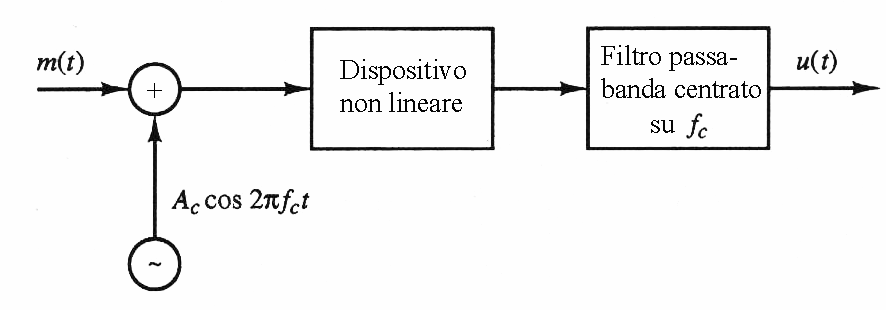
\includegraphics[scale = 0.6]{AM Convenzionale utilizzando un filtro passa-banda e un dipositivo non lineare.png}
\end{figure} 

l'uscita u(t) risulta, con le dovute semplificazioni: 

{
    \Large 
    \begin{equation}
        u(t)
        = 
        A_c a_1 \left[1 + \frac{2a_2}{a_1} m(t)\right] \cos(2 \pi f_c t)
    \end{equation}
}

u(t) ha le caratteristiche di un segnale modulato in ampiezza in modo convenzionale, 
i.e. AM convenzionale. \newline 

Inoltre, sapendo che u(t) è un segnale convenzionale, il termine $1 + \frac{2a_2}{a_1} m(t)$ non può essere negativo. \newline 

Grazie alla funzione caratteristica del diodo, che appunto è un dispositivo non lineare, 
è possibile realizzare uno "Switching Modulator", da cui si ottiene una modulazione AM-convenzionale, 
che ha il seguente schema circuitale: 

\begin{figure}[h]
    \centering
    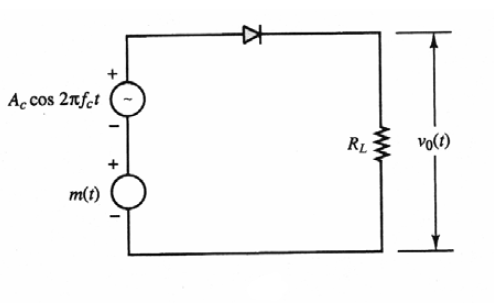
\includegraphics[scale = 1]{Switching Modulator schema circuitale.PNG}
\end{figure} 

oppure è possibile realizzare un "Ring Modulator", da cui si ottiene una modulazione DSB-SC, 
che ha il seguente schema circuitale: 

\begin{figure}[h]
    \centering
    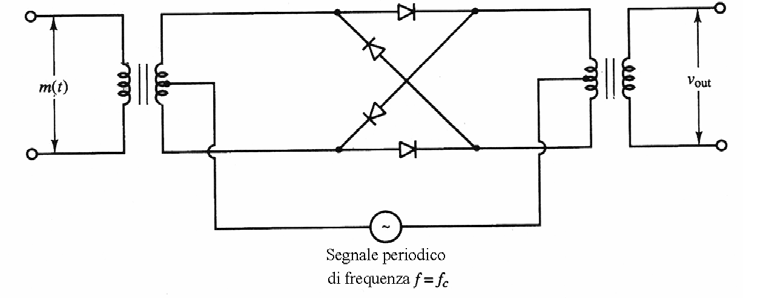
\includegraphics[scale = 1]{Ring Modulator schema circuitale.PNG}
\end{figure} 

Per lo schema dello "Switching Modulator" e del "Ring Modulator", 
il principio di funzionamento è quello di moltiplicare il segnale modulante m(t) per una funzione periodica p(t) di periodo $\frac{1}{f_c}$. \newline 

p(t), sviluppata in serie di Fourier, conterrà anche la componente di interesse a frequenza $f_c$. \newline 

Ad esempio l'uscita del circuito del Ring Modulator, che nel tempo ha questo andamento: 

\begin{figure}[h]
    \centering
    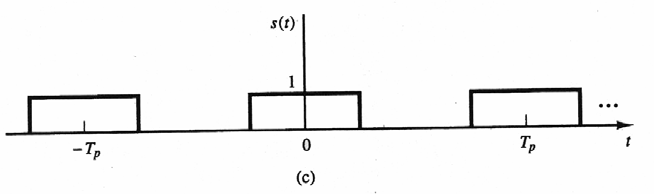
\includegraphics[scale = 1]{Andamento nel tempo tensione uscita Ring Modulator.png}
\end{figure} 


può essere scritta matematicamente come: 

{
    \Large 
    \begin{equation}
        \begin{split}
            v_0 (t) 
            &= 
            m(t) \cdot p(t)
            \\
            &= 
            m(t)
            \frac{4}{\pi} 
            \sum_{n = 1}^{+ \infty}
            \frac{(-1)^{n-1}}{2n - 1 }
            \cos [2 \pi f_c (2n - 1)]
        \end{split}
    \end{equation}
}

Come al solito, la componente di interesse può essere isolata utilizzando, a valle, un opportuno filtro passa-banda. \newline 

Un segnale DSB-SC può anche essere ottenuto combinando due modulatori identici AM convenzionali in uno schema bilanciato, come illustrato con la seguente figura: 

\begin{figure}[h]
    \centering
    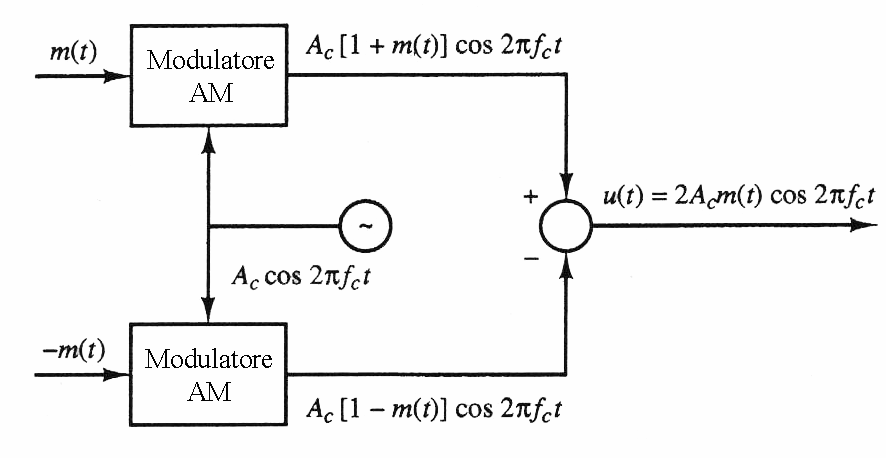
\includegraphics[scale = 0.8]{Architettura DSB-SC partendo da modulatori AM.png}
\end{figure} 

\begin{tcolorbox}
    Chiaraluce potrebbe tranquillamente, a mio parere, far insegnare un corso di Elettronica Analogica. Fine
\end{tcolorbox}

\newpage 

\section{Modulazione angolare}
\footnote{Slide del prof | Modulazioni analogiche | pag 18 - 21\\  
Appunti di Damiano| pag 18 - 21\\
Appunti | Modulazioni analogiche | pag 18 - 21\\
Appunti | 2025-03-04 | pag 8 - 9 \\
Appunti | 2025-03-07 | pag 2 
} 

Ricordando che un segnale c(t) (carrier, cioè segnale di portante) sinusoidale può essere descritto dalla seguente equazione: 

{
    \Large 
    \begin{equation}
        c(t) = A_c \cdot \cos(2 \pi f_c t + \phi_c)
    \end{equation}
}

il segnale della portante c(t) può, non solo modificare l'ampiezza del segnale modulante m(t), 
ma anche modificare la fase $\phi_c$ o la frequenza $f_c$. \newline 

In particolare, si parla di modulazione in fase PM (Phase Modulation) se il segnale modulato risulta: 

{
    \Large 
    \begin{equation}
        \begin{split}
            u(t)
            &= 
            A_c \cos(\theta (t))
            \\
            &= 
            A_c \cos(2 \pi f_c t + \phi(t))
        \end{split}
    \end{equation}
}

in cui: 

{
    \Large 
    \begin{equation}
        \phi (t) = k_p m(t)
    \end{equation}
}

dove $k_p$ è definito come costante di deviazione di fase. \newline 

Nella modulazione di fase, viene modificata $\phi$ in funzione del segnale modulante m(t) in maniera proporzionale. \newline 

Viene definita la frequenza istantanea del segnale u(t) come: 

{
    \Large 
    \begin{equation}
        \begin{split}
            f_i (t)
            &= 
            \frac{1}{2 \pi }
            \frac{d \theta(t)}{dt}
            \\
            &= 
            \frac{1}{2 \pi }
            \frac{d}{dt}
            (2 \pi f_c t + \phi (t))
            \\
            &= 
            f_c + f_c \frac{1}{2 \pi} \frac{d \phi (t)}{dt}
        \end{split}
    \end{equation}
}

$f_i (t)$ viene definita come modulazione di frequenza FM (Frequency Modulation) se risulta: 

{
    \Large 
    \begin{equation}
        f_i (t) - f_c = k_f m(t)
    \end{equation}
}

dove $k_f$ è definita come costante di deviazione di frequenza. \newline 

In altri termini, viene definita modulazione di frequenza quando la differenza rispetto a $f_c (t)$ è proporzionale a m(t) segnale modulante. \newline 

Se: 

{
    \Large 
    \begin{equation}
        m(t) = 0
    \end{equation}
}

nella modulazione di frequenza si trasmette solo $f_c(t)$, cioè la portante. \newline 

La modulazione FM e PM sono strettamente legate: 
dove esiste una esiste l'altra e viceversa. \newline 

In effetti. integrando l'espressione di $f_i (t)$ e tenendo conto dell'espressione di $k_f m(t)$, 
possiamo esprimere la fase $\phi (t)$ come: 

{
    \Large 
    \begin{equation}
        \phi (t)
        = 
        2 \pi k_f 
        \int_{- \infty}^{t}
        m (\tau) d\tau
    \end{equation}
}

A sua volta, derivando: 

{
    \Large 
    \begin{equation}
        \phi (t) = k_p m(t)
    \end{equation}
}

e tenendo conto dell'espressione di $f_i (t)$, 
si conclude che la PM è esprimibile come FM se: 

{
    \Large 
    \begin{equation}
        f_i (t) - f_c 
        =
        \frac{1}{2 \pi} k_p \frac{d}{dt} m(t)
    \end{equation}
}

In base a queste due espressioni, possiamo dire che la FM può essere vista come una PM in cui m(t) viene integrato, 
invece la PM può essere vista come una FM in cui m(t) viene derivata. \newline 

Ricapitolando si parla di FM o PM quando: 

{
    \Large 
    \begin{equation}
        \phi (t)
        = 
        \begin{cases}
            \begin{array}{ll}
            k_p m(t) & \textbf{ PM} 
            \\
            \\
            2 \pi k_f \int_{-\infty}^{t} m(\tau) d\tau & \textbf{ FM}
            \end{array} 
        \end{cases}
    \end{equation}
}

e 

{
    \Large 
    \begin{equation}
        f_i (t) - f_c
        = 
        \begin{cases}
            \begin{array}{ll}
            \frac{1}{2 \pi} k_p \frac{d}{dt} m(t) & \textbf{ PM} 
            \\
            \\
            k_f m(t) & \textbf{ FM}
            \end{array} 
        \end{cases}
    \end{equation}
}

Queste considerazioni danno un'indicazione esplicita su come realizzare il modulatore. \newline 

\newpage 

Come viene spiegato dalle seguenti figure: 

\begin{figure}[h]
    \centering
    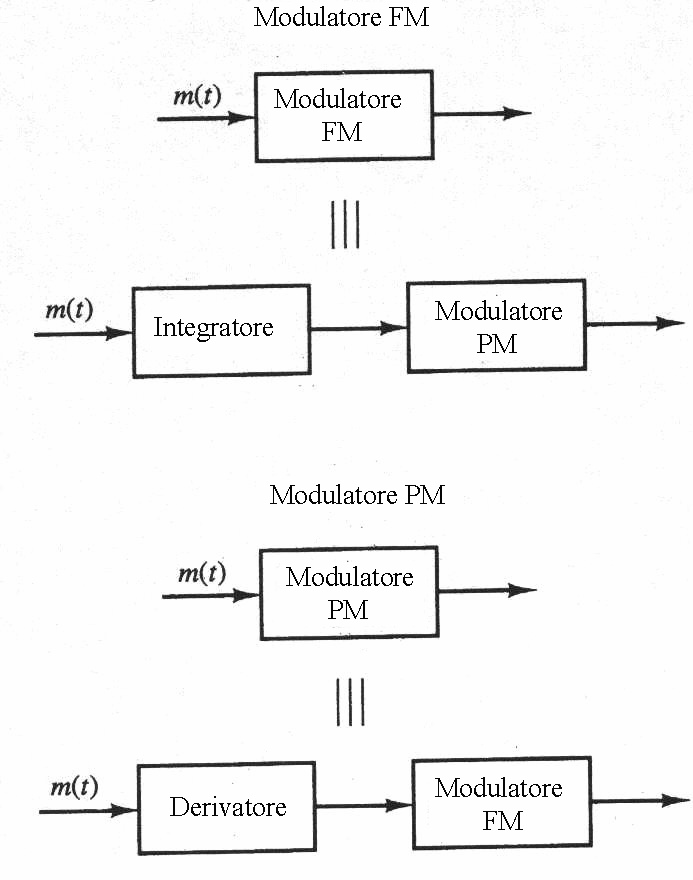
\includegraphics[scale = 0.8]{Modulatore FM e PM interscambiabili.png}
\end{figure} 

con l'aggiunta di un circuito o integratore o derivatore, 
è possibile realizzare un modulatore FM o PM partendo dal suo reciproco. \newline 

\newpage

Inoltre, visualizzando i segnali di ingresso e quelli di uscita dei modulatori: 

\begin{figure}[h]
    \centering
    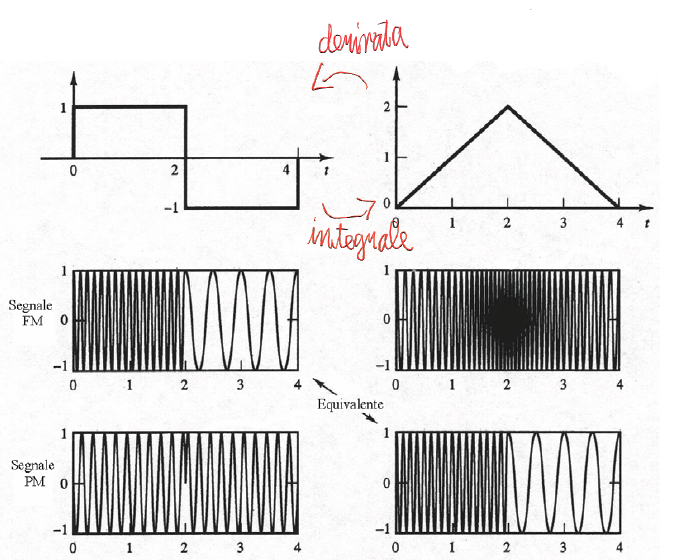
\includegraphics[scale = 1]{Andamenti segnali FM e PM.PNG}
\end{figure} 

possiamo osservare che i segnali FM e PM, con le osservazioni svolte, sono equivalenti. \newline 

Stabilita questa corrispondenza tra le due tecniche di modulazione, si può parlare genericamente di modulazione angolare. \newline 

\newpage 

\subsection{Indici della modulazione angolare}
\footnote{Slide del prof | Modulazioni analogiche | pag 21 - 23\\  
Appunti di Damiano| pag 21 - 23\\
Appunti | Modulazioni analogiche | pag 21 - 23\\
Appunti | 2025-03-07 | pag 2 - 3
} 

Per il fatto che il segnale modulante agisce sull'argomento della portante, 
la modulazione angolare è più difficile da trattare rispetto alla modulazione in ampiezza. \newline 

La modulazione di ampiezza è molto semplice: basta traslare lo spettro del segnale in BB a frequenza di portante. \newline 

Invece questo fatto, nelle angolazioni angolari, non avviene; alche la modulazione angolare è definita come modulazione non lineare, a differenza di quella di ampiezza. \newline 

Per questo motivo, molti dei calcoli relativi alla modulazione angolare sono stati preventivati considerando, 
come segnale modulante, il segnale sinusoidale. \newline 

Per una modulante sinusoidale: 

{
    \Large 
    \begin{equation}
        m(t) = a \cos(2 \pi f_m t)
    \end{equation}
}

si definisce come indici di modulazione, rispettivamente di fase $\beta_p$ e di frequenza $\beta_f$, come segue: 

{
    \Large 
    \begin{equation}
        \beta_p = k_p a
    \end{equation}
}

{
    \Large 
    \begin{equation}
        \beta_f = \frac{k_f a}{f_m}
    \end{equation}
}

Grazie a questi indici, possiamo esprimere il segnale modulato u(t) come: 

{
    \Large 
    \begin{equation}
        u(t)
        = 
        \begin{cases}
            \begin{array}{ll}
            A_c \cos \left[ 2 \pi f_c t + \beta_p \cos(2 \pi f_m t)\right] & \textbf{ PM} 
            \\
            A_c \cos \left[ 2 \pi f_c t + \beta_f \sin(2 \pi f_m t)\right] & \textbf{ FM}
            \end{array} 
        \end{cases}
    \end{equation}
}

È immediato verificare che $k_p a$ rappresenta la massima deviazione di fase $\Delta \phi_{max}$: 

{
    \Large 
    \begin{equation}
        \Delta \phi_{max}
        = 
        k_p \max \abs{m(t)}
    \end{equation}
}

nella PM. \newline 

Invece nella FM, $k_f a$ rappresenta la massima deviazione di frequenza $\Delta f_{max}$: 

{
    \Large 
    \begin{equation}
    \Delta f_{max}
        = 
        k_f \max \abs{m(t)}
    \end{equation}
} 

Grazie a queste definizioni, possiamo riscrivere $\beta_p$ e $\beta_f$ come: 

{
    \Large 
    \begin{equation}
        \beta_p = \Delta \phi_{max}
    \end{equation}
}

{
    \Large 
    \begin{equation}
        \beta_f = \frac{\Delta f_{max}}{f_m}
    \end{equation}
}

Originariamente introdotte per il caso di segnale modulante sinusoidale, 
le definizioni di $\beta_p$ e $\beta_f$ possono essere estese ad un segnale modulante qualsiasi, 
a patto di sostituire $f_m$ con la sua larghezza di banda W. \newline 

Formalmente, per la PM, per un segnale qualsiasi modulante di larghezza di banda W, rimane uguale a prima, quindi: 

{
    \Large 
    \begin{equation}
        \beta_p = \Delta \phi_{max}
    \end{equation}
}

invece, per la FM, diventa: 

{
    \Large 
    \begin{equation}
        \beta_f = \frac{\Delta f_{max}}{W}
    \end{equation}
}

Se un segnale avesse più frequenze, bisogna considerare la banda totale del segnale modulante W. \newline 

\newpage 


\subsubsection{Modulazione angolare a basso indice}
\footnote{Slide del prof | Modulazioni analogiche | pag 23 - 24\\  
Appunti di Damiano| pag 23 - 24\\
Appunti | Modulazioni analogiche | pag 23 - 24\\
Appunti | 2025-03-07 | pag 3 - 4\\
Appunti | 2025-07-08 Ricevimento | pag 10
} 

L'indice di modulazione $\beta$ è un parametro fondamentale della modulazione angolare 
e svolge un ruolo chiave nella qualità di trasmissione quando il segnale è affetto da rumore. \newline 

Si parla di modulazione angolare a basso indice (o modulazione angolare a banda stretta)
quando la variazione di $\phi (t)$: 

{
    \Large 
    \begin{equation}
        \phi (t)
        = 
        \begin{cases}
            \begin{array}{ll}
            k_p m(t) & \textbf{ PM} 
            \\
            \\
            2 \pi k_f \int_{-\infty}^{t} m(\tau) d\tau & \textbf{ FM}
            \end{array} 
        \end{cases}
    \end{equation}
}

risulta molto piccola, cioè: 

{
    \Large 
    \begin{equation}
        \phi (t) << 1
    \end{equation}
}

Sotto questa ipotesi, il segnale modulato con modulazione angolare da: 

{
    \Large 
    \begin{equation}
        \begin{split}
            u(t)
            &= 
            A_c \cos(\theta (t))
            \\
            &= 
            A_c \cos(2 \pi f_c t + \phi(t))
        \end{split}
    \end{equation}
}

diventa: 

{
    \Large
    \begin{equation}
        \begin{split}
        u(t)
        &= 
        A_c \cos(2 \pi f_c t + \phi (t))   
        \\
        &= 
        A_c \cos(2\pi f_c t) \cos(\phi (t)) 
        - 
        A_c \sin(2\pi f_c t) \sin(\phi (t))
        \\
        &\approx
        A_c \cos(2\pi f_c t)  
        - 
        A_c \sin(2\pi f_c t) \phi (t)
        \\
        &= 
        A_c \cos(2\pi f_c t)  
        - 
        A_c \phi (t) \sin(2\pi f_c t) 
    \end{split}
    \end{equation}
}

\begin{tcolorbox}
Non dobbiamo impararci le formule a memoria. \newline 

Dobbiamo solo sapere che l'informazione è contenuta nella fase $\phi (t)$. \newline

    Dall'analisi matematica 1, 
    si è potuto approssimare $\sin(\phi(t))$ a $\phi (t)$ grazie alla teoria degli o-piccoli. \newline 

    Ripassino al volo che non fa mai male: \\
    \url{https://www.youmath.it/lezioni/analisi-matematica/limiti-continuita-e-asintoti/3247-o-piccolo.html}
\end{tcolorbox}

Questa espressione di u(t) esplicita la somiglianza con l'espressione di un segnale modulato in AM convenzionale: 

{
    \Large 
    \begin{equation} 
        \begin{split}
        u (t)
        &= 
        A_c 
        [1 + \alpha \cdot m_n (t)] 
        \cos(2 \pi f_c t + \phi_c)
        \\
        &= 
        A_c \cos(2 \pi f_c t + \phi_c)
        +
        A_c \alpha \cdot m_n (t) \cos(2 \pi f_c t + \phi_c)
        \end{split}
    \end{equation}
}

\newpage 

Utilizzando il piano dei fasori, 
possiamo graficare le due espressione di u(t): 

\begin{figure}[h]
    \centering
    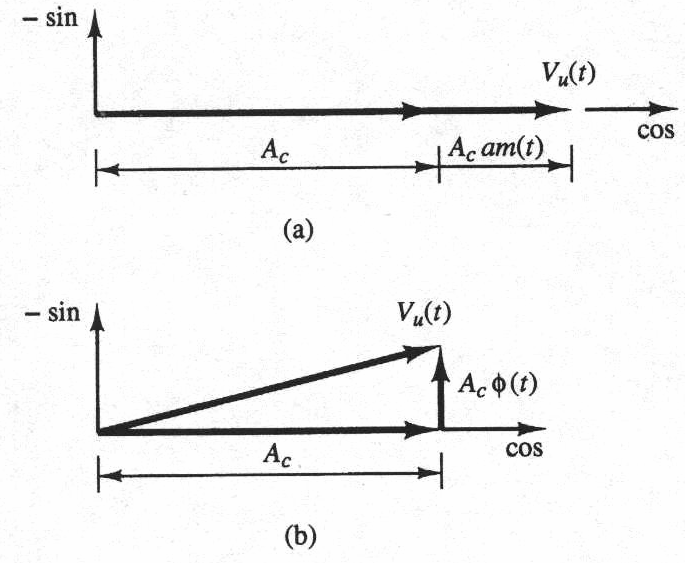
\includegraphics[scale = 1]{Confronto nel piano fasoriale tra AM e modulazione angolare a basso indice.png}
\end{figure} 

dove la prima in alto è u(t) con modulazione AM-convenzionale, 
invece la seconda in basso è u(t) con modulazione angolare a basso indice. \newline 

Si può svolgere la seguente osservazione: 
nella AM convenzionale, il modulo di $V_u (t)$ varia in base alla modulazione (vedo m(t) che si trova sul piano del coseno) e il suo angolo rimane costante; 
invece, nella modulazione angolare, abbiamo che il modulo di $V_u (t)$ rimane costate, ma varia il suo angolo (vedi $\phi (t)$ sul piano del seno). \newline 

Per fissare bene le idee, consideriamo al caso PM in cui il segnale modulato vale: 

{
    \Large 
    \begin{equation}
        u(t) 
        \approx
        A_c \cos(2 \pi f_c t)
        - 
        A_c k_p m(t) \sin(2 \pi f_c t) 
    \end{equation}
}

Facendo la trasformata di Fourier di u(t) e considerando m(t) reale pari, sapendo le proprietà tra trasformata di Fourier nel tempo e in frequenza anche M(f) sarà a sua volta reale pari, 
possiamo visualizzare U(f) come: 

\begin{figure}[h]
    \centering
    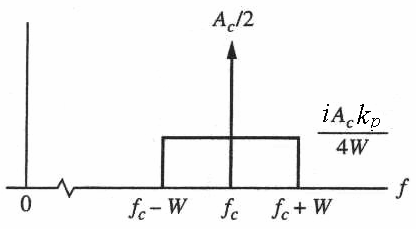
\includegraphics[scale = 1]{Segnale PM modulato a basso indice in Fourier.png}
\end{figure} 

dove in figura si considerano solo le frequenze positive. \newline 

Si parla di modulazione angolare a banda stretta perché, come si visualizza in figura, 2W è la minima occupazione 
spettrale conseguibile in modulazione angolare, quindi PM e FM, e si ottiene sono nell'ipotesi di: 

{
    \Large 
    \begin{equation}
        \phi (t) << 1
    \end{equation}
}

\newpage 

\subsection{Banda di una modulazione angolare}
\footnote{Slide del prof | Modulazioni analogiche | pag 25 - 26\\  
Appunti di Damiano| pag 25 - 26\\
Appunti | Modulazioni analogiche | pag 25 - 26\\
Appunti | 2025-03-07 | pag 4
} 

Assumendo per il segnale modulante m(t) una funzione cosinusoidale con frequenza $f_m$, 
si può scrivere: 

{
    \Large 
    \begin{equation}
        u(t) 
        = 
        A_c 
        \cos(2 \pi f_c t + \beta \cos(2 \pi f_m t))
    \end{equation}
}

con $\beta = \beta_p$ se si fa una PM o $\beta = \beta_f$ se si fa una FM. \newline 

Visto che analiticamente è difficile svolgere un coseno dentro ad un coseno, 
u(t) può essere riscritta come: 

{
    \Large 
    \begin{equation}
        u(t)
        = 
        \sum_{n = -\infty}^{+ \infty}
        A_c 
        J_n (\beta) \cos \left[ 2 \pi (f_c + n f_m) t\right]
    \end{equation}
}

dove $J_n (\beta)$ è la funzione di Bessel di prima specie di ordine n. \newline 

\begin{tcolorbox}
    Cosa sono e perché si utilizzano in casi particolari le funzioni di Bessel? \newline 

    \url{https://it.wikipedia.org/wiki/Equazioni_di_Bessel}
\end{tcolorbox}

Alcuni andamenti di $J_n (\beta)$: 

\begin{figure}[h]
    \centering
    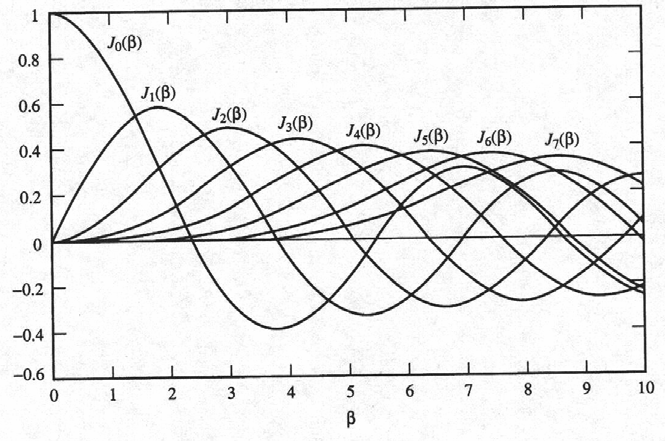
\includegraphics[scale = 1]{Funzioni di Bessel.png}
\end{figure}

Sulla base della formula di u(t), notiamo che u(t) è esprimibile con una sommatoria di infiniti termini, 
in cui avremo, nello spettro, infinite armoniche, quindi infinite righe ogni frequenza multipla di $f_m$. \newline 

Per questo motivo la modulazione angolare non viene definita lineare come la modulazione in ampiezza, 
perché, in questo caso, lo spettro in BB non viene semplicemente traslato alla frequenza della portante. \newline 

Inoltre, sapendo che la potenza del segnale modulato è costante a pari a $\frac{A_c ^{2}}{2}$ (dalle proprietà di ciclo-stazionarietà dello spettro in frequenza), 
si può dire che la potenza delle funzioni di Bessel vale: 

{
    \Large 
    \begin{equation}
        \sum_{n = - \infty}^{+ \infty}
        \left[ J_n (\beta)\right]^{2} = 1
    \end{equation}
}

Questa è una proprietà delle funzioni di Bessel di prima specie. \newline 

L'occupazione illimitata della banda non consentirebbe un utilizzo pratico del sistema. \newline 

Se però si visualizza l'andamento delle funzioni di Bessel, si nota che, per ogni valore di $\beta$, 
c'è un numero limitato di funzioni di Bessel che danno un contributo significativo. \newline 

In particolare, risulta applicabile la regola secondo cui le funzioni di Bessel di ordine n: 

{
    \Large 
    \begin{equation}
        n \le \beta + 1
    \end{equation}
}

sono apprezzabilmente diverse da zero. \newline 

Invece le funzioni di Bessel di ordine n: 
{
    \Large 
    \begin{equation}
        n > \beta + 1
    \end{equation}
} 

sono trascurabili. \newline 

Sulla base di queste considerazioni, si può concludere che delle infinite armoniche nominalmente presenti nello spettro del segnale modulato 
danno, in realtà, contributo significativo allo spettro solo quelle che distano dalla portante non più di $(\beta + 1)$ volte $f_m$. \newline 

Tenendo conto della distribuzione bilatera rispetto alla portante, ne risulta una banda "effettiva" occupata dalla modulazioni angolari di: 

{
    \Large 
    \begin{equation}
        B_c = 2 (\beta + 1) f_m
    \end{equation}
}

$B_c$ contiene il 98 \% della potenza totale del segnale. \newline 

Sapendo la relazione tra $\beta$ e $B_c$, possiamo esprimere $B_c$ per le due modulazioni angolari studiate: 

{
    \Large 
    \begin{equation}
        B_c
        = 
        \begin{cases}
            \begin{array}{ll}
            2 (k_p a + 1) f_m & \textbf{ PM} 
            \\
            2 (k_f a + f_m) & \textbf{ FM}
            \end{array} 
        \end{cases}
    \end{equation}
}

dove a è l'ampiezza del segnale modulante. \newline 

Da queste due formule di $B_c$ per PM e FM si nota che all'aumentare di a, aumenta $B_c$ sia nella PM che nella FM. \newline 

Invece, $f_m$ nella PM moltiplica il termine $2(k_p a + 1)$, 
invece nella FM, $f_m$ ha un ruolo additivo al termine $k_f a$. \newline 

Quindi, all'aumentare di $f_m$, la banda $B_c$ aumenta nettamente di più nella PM rispetto alla FM. \newline 

Queste formule della banda $B_c$ sono valide per un segnale modulante cosinusoidale. \newline 

\newpage

\subsubsection{Banda di una modulazione angolare per un segnale modulante qualsiasi}
\footnote{Slide del prof | Modulazioni analogiche | pag 26 - 27\\  
Appunti di Damiano| pag 26 - 27\\
Appunti | Modulazioni analogiche | pag 26 - 27\\
Appunti | 2025-03-07 | pag 4 - 5
}

Nel caso in cui si considera un generico segnale periodico (che possiamo generalizzare come caso di modulante cosinusoidale) 
e un processo gaussiano (esemplificativo di una funzione stocastica), si possono adattare i parametri visti precedente a questo caso. \newline 

La formula di $B_c$ vista precedentemente è valida se a $f_m$ si sostituisce la frequenza massima significativa W dello spettro del segnale modulante:
: 

{
    \Large 
    \begin{equation}
        \begin{split}
        B_c
        &= 
        \begin{cases}
            \begin{array}{ll}
            2 (k_p a + 1) f_m & \textbf{ PM} 
            \\
            2 (k_f a + f_m) & \textbf{ FM}
            \end{array} 
        \end{cases}
        \\
        &\downarrow
        \\
        B_c
        &= 
        \begin{cases}
            \begin{array}{ll}
            2 (k_p a + 1) W & \textbf{ PM} 
            \\
            2 (k_f a + W) & \textbf{ FM}
            \end{array} 
        \end{cases} 
        \end{split}
    \end{equation}
}


Lo stesso principio vale per l'altra formula di $B_c$: 

{
    \Large 
    \begin{equation}
        \begin{split}
            B_c &= 2 (\beta + 1) f_m 
        \\
        &\downarrow
        \\
        B_c &= 2 (\beta + 1) W
        \end{split}
    \end{equation}
}

Queste formula di $B_c$ costituisce una eccellente approssimazione della banda occupata da un segnale in modulazione angolare. \newline 

Questa formula è universalmente nota come "regola di Carson". \newline 

Ma, è bene precisare che, la formula di Carson nel caso FM, così calcolata, è una sottostima di $B_c$ se il valore di $\beta$ 
è compreso tra 2 e 10. \newline 

Quindi la formula di Carson, in questo caso particolare diventa: 

{
    \Large 
    \begin{equation}
        B_c = 2 (\beta_f + 2 ) W \textbf{ FM per  $ 2 < \beta_f < 10$ }
    \end{equation}
}

\newpage 

\subsection{Mo/demodulatori angolari}
\footnote{Slide del prof | Modulazioni analogiche | pag 27 - 31\\  
Appunti di Damiano| pag 27 - 31\\
Appunti | Modulazioni analogiche | pag 27 - 31\\
Appunti | 2025-03-10 | pag 2 - 4\\ 
Appunti | 2025-07-08 Ricevimento | pag 10
} 

Dalla formula della modulazione angolare PM a basso indice u(t): 

{
    \Large 
    \begin{equation}
        u(t) 
        \approx
        A_c \cos(2 \pi f_c t)
        - 
        A_c k_p m(t) \sin(2 \pi f_c t) 
    \end{equation}
}

possiamo dire che la modulazione angolare può essere vista come una modulazione AM-convenzionale con uno shift di $90^{\circ}$
(il seno rispetto al coseno differiscono di $90^{\circ}$) della portante. \newline 

Grazie a questa osservazione, possiamo costruire il seguente schema del modulatore angolare: 

\begin{figure}[h]
    \centering
    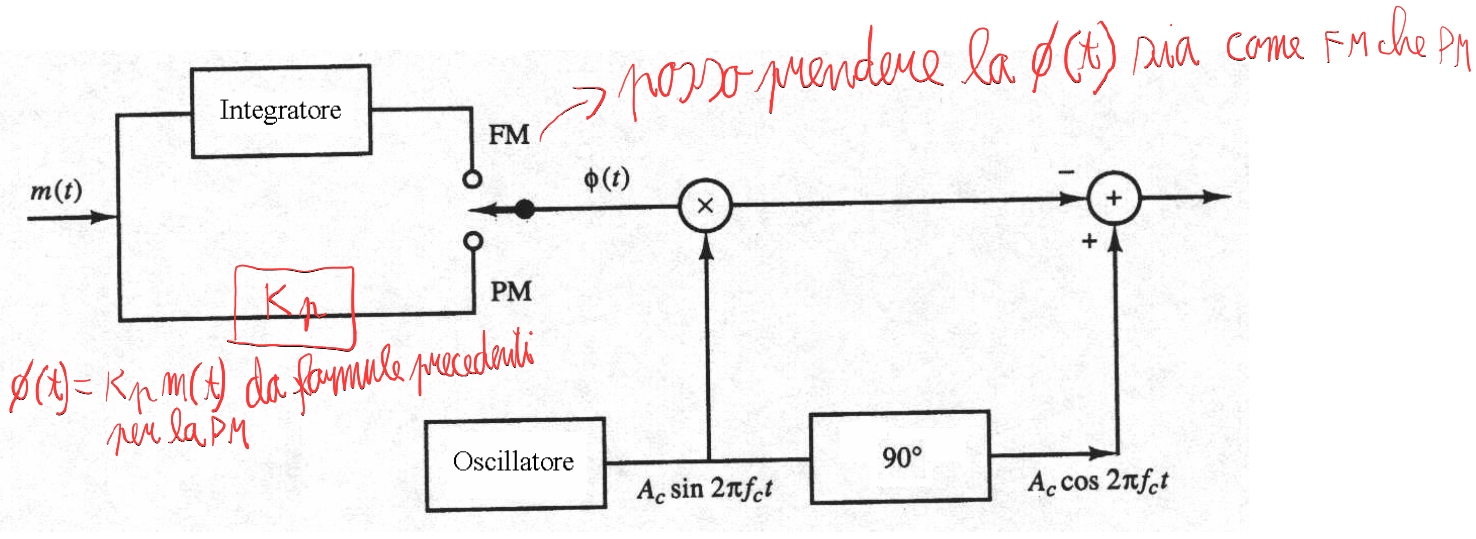
\includegraphics[scale = 0.6]{Modulatore di Armstrong.PNG}
\end{figure}

Questo tipo di modulatore angolare è definito come modulatore di Armstrong. \newline 

Invece, per un segnale FM, non necessariamente a basso indice, si ottiene utilizzando un diodo varactor o chiamato anche oscillatore in tensione (VCO: Voltage Controlled Oscillator). \newline 

Un possibile circuito per modulare un segnale FM a basso indice: 

\begin{figure}[h]
    \centering
    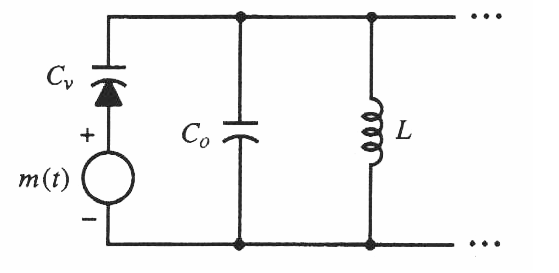
\includegraphics[scale = 0.8]{VCO.png}
\end{figure}

\begin{tcolorbox}
Quel componente segnato come $C_v$ che sembra sia un diodo che una capacità è un capacitore variabile che cambia il suo valore di capacità in base alla tensione ai suoi capi, 
in questo circuito $C_v$ cambia la sua capacità in base alla tensione di m(t) 
\end{tcolorbox}

Un altro circuito per generare un segnale FM o PM con indice di modulazione $\beta$ generico 
è quello del narrowband angle modulator, che fa riferimento al modulatore di Armstrong ma a banda stretta. \newline 

\newpage 

Di seguito, il disegno dell'architettura: 

\begin{figure}[h]
    \centering
    \includegraphics[scale = 0.8]{Narrowband angle modulator architettura.png}
\end{figure}

L'introduzione dell'oscillatore locale a frequenza $f_{LO}$ è dovuta alla necessità di allocare il segnale trasmesso alla frequenza di portante desiderata, 
ove tale non fosse il risultato della moltiplicazione di $n \cdot f_c$. \newline 

L'oscillatore locale serve per una conversione in frequenza. \newline 

Il filtro passa-banda toglie tutte le componenti che non sono necessarie. \newline 

La tecnica che applica questo tipo di architettura circuitale prende il nome di metodo indiretto. \newline 

\newpage 

\subsubsection{Demodulatori angolari}
\footnote{Slide del prof | Modulazioni analogiche | pag 28 \\  
Appunti di Damiano| pag 28 \\
Appunti | 2025-03-10 | pag 2 \\
Appunti | 2025-07-08 Ricevimento | pag 9
} 

Benché, in linea di principio, la demodulazione di un segnale PM o FM possa essere realizzata con tecniche coerenti (quindi moltiplicando per delle funzioni cosinusoidali), 
in grado di estrarre la fase del segnale (in cui è associata l'informazione), 
in pratica si preferisce di adottare tecniche non coerenti, in modo da semplificare drasticamente la struttura del ricevitore. \newline 

Consideriamo il caso solo della demodulazione in FM, sapendo che il demodulatore FM può essere anche un demodulatore PM. \newline 

L'idea è quella di convertire il segnale FM in segnale AM-convenzionale prima di procedere alla demodulazione. \newline 

Lo schema del demodulatore FM è il seguente: 

\begin{figure}[h]
    \centering
    \includegraphics[scale = 0.8]{Demodulatore FM.png}
\end{figure}

in cui il convertitore FM/AM è un banale derivatore. \newline 

Ora andiamo a calcolare analiticamente la demodulazione. \newline 

Un possibile schema di un convertitore FM/AM: 

\begin{figure}[h]
    \centering
    \includegraphics[scale = 0.8]{Convertitore FM-AM.png}
\end{figure}

Consideriamo il segnale in ingresso u(t) modulato: 

{
    \Large 
    \begin{equation}
        u(t)
        = 
        A_c 
        \cos 
        \left(
            2 \pi f_c t 
            + 
            2 \pi k_f \int_{- \infty}^{t} m(\tau) d\tau
        \right)
    \end{equation}
}

La funzione di trasferimento H(f) di un blocco derivatore è caratterizzato dalle seguente funzione: 

{
    \Large
    \begin{equation}
        \abs{H(f)} = V_0 + k(f - f_c) \textbf{ per } \abs{f - f_c} \le \frac{B_c}{2}
    \end{equation}
}

\begin{tcolorbox}
Dalle relazioni tra dominio del tempo e frequenza, 
una derivata nel tempo, dobbiamo avere un funzione lineare nell'intorno della frequenza da considerare, 
in questo caso nell'intorno di $f_c$. \newline 

Per realizzare questo filtro derivatore, si usano dei circuiti risonanti e si trova il loro tratto lineare. \newline 

Essendo circuiti risonanti composti da induttori, questi permettono di svolgere delle derivate nel tempo, 
grazie alla loro funzione caratteristica. 
\end{tcolorbox}

Per il resto, si tratta di una funzione puramente immaginaria, e dunque asimmetrica rispetto all'origine. \newline 

Il segnale che esce fuori dopo il filtro è: 

{
    \Large 
    \begin{equation}
        v_0 (t)
        = 
        - A_c 
        \left[
            V_0 + k k_f m(t)
        \right]
        \sin 
        \left(
            2 \pi f_c t 
            + 
            2 \pi k_f 
            \int_{-\infty}^{t} m(\tau) d\tau
        \right)
    \end{equation}
}

Il rivelatore di inviluppo estrae dalla funzione di $v_0 (t)$ l'argomento $- A_c 
        \left[
            V_0 + k k_f m(t)
        \right]$

\newpage




\include{Qualità nelle modulazioni analogiche}
\chapter{Conversione AD}

\begin{figure}[h]
    \centering
    \includegraphics[scale = 1]{campdig.jpg}
\end{figure}

\newpage 

\section{Quantizzazione}
\footnote{Slide del prof | Conversione AD | pag 1.1 
}

Data una funzione analogica, cioè una funzione con infiniti valori sia nel tempo che nelle ascisse, 
la si vuole discretizzare in modo da essere reinterpretata dai circuiti digitali. \newline 

Per discretizzarla sull'asse dei tempi, alla funzione deve essere applicato il campionamento. \newline 

\begin{tcolorbox}
    Argomento ripreso da quasi tutti i corsi di ingegneria elettronica. \newline 

    Da  \url{https://github.com/ciccio25/appunti-misure-elettroniche} \\
    Capitolo 7.4 Teorema fondamentale del campionamento | pag 112 \newline 

    Per il campionamento, è stato rivoluzionario il teorema del campionamento scritto dal matematico 
    Claude. \newline 

Di seguito il teorema fondamentale del campionamento: 

\includegraphics[scale = 0.5]{Teorema fondamentale del campionamento originale.PNG}

\begin{tcolorbox}
    Shannon pubblicò il suo teorema nella seguente rivista: 
    "Claude E. Shannon Communication in the Presence of Noise
Proceedings of the IRE, vol. 37, no. 1, pp. 10-21, Jan. 1949" 
consultabile al seguente link \\ \url{https://webusers.imj-prg.fr/~antoine.chambert-loir/enseignement/2020-21/shannon/shannon1949.pdf}
\end{tcolorbox}

Visto che il teorema è stato pubblicato nel 1949, alcune terminologie sono diverse da quello al giorno d'oggi. \newline 

Le seguenti terminologie sono: 

\begin{itemize}
    \item cps è un'abbreviazione di cycles per second, nei giorni odierni utilizziamo l'indicazione di Hz 
    \item per ordinates si intendono i valori istantanei 
\end{itemize}

La traduzione italiana, con i seguenti adattamenti, del teorema fondamentale del campionamento è la seguente: \newline 

Se la funzione f(t) contiene nessuna frequenza maggiore di W Hz, è completamente determinata dai 
suoi valori istantanei spaziati da una serie di punti spaziati di $\frac{1}{2W}$ secondi tra di loro. \newline 

Questo teorema ci dice che, se gli istanti di campionamento sono opportunamente individuati, 
la funzione che si ottiene andando a prelevare il valore istantaneo del segnale solo in quegli istanti, 
è completamente determinata, quindi non si ha perdita di informazione. \newline 

\end{tcolorbox}

Una volta che la funzione è campionata, quindi è discretizzata nell'asse dei tempi, la si può discretizzare nell'asse delle ascisse. \newline 

La discretizzazione nell'asse delle ascisse prende il nome di quantizzazione. \newline

\newpage 

Possiamo graficare i processi di discretizzazione svolti con questa figura: 

\begin{figure}[h]
    \centering
    \includegraphics[scale = 1]{campdig.jpg}
\end{figure}

\begin{tcolorbox}
    Per chi come me ha svolto prima o ha seguito le lezioni del terzo anno di Misure Elettroniche della mitica prof.ssa Spinsante, 
    alcune terminologie sono differenti, ma alla fine andiamo a finire negli stessi argomenti sotto l'occhio non di un misurista, 
    bensì di un telecomunicazionista
\end{tcolorbox}

La discretizzazione può essere di due tipi, in base a come si divide l'asse delle ordinate: 

\begin{itemize}
    \item quantizzazione scalare, ogni intervallo è costante 
    \item quantizzazione non uniforme, ogni intervallo non è costante rispetto agli altri
\end{itemize}

\begin{tcolorbox}
    Per tutta la quantizzazione, rimando al corso di Misure elettroniche dove è spiegato benissimo. \newline  
    
    Da  \url{https://github.com/ciccio25/appunti-misure-elettroniche} \\
    Capitolo 7.8 Fase 2: Quantizzazione | pag 122 - 124 \newline 

    Nel corso di Misure Elettroniche, abbiamo affrontato solo la quantizzazione scalare. 
\end{tcolorbox}

\newpage 

\section{Quantizzazione scalare}
\footnote{Slide del prof | Conversione AD | pag 1.1 \\ 
Slide | Conversione AD | pag 1.1 
}


Data una funzione già campionata, possiamo applicare una quantizzazione scalare. \newline 

In questo tipo di quantizzazione, si associa un valore x a un valore $\hat{x_i}$, che a sua volta ricade in un valore nelle ordinate $a_i$. \newline 

Come si visualizza dalla seguente figura: 

\begin{figure}[h]
    \centering
    \includegraphics[scale = 1]{Quantizzazione scalare N = 8.png}
\end{figure} 

Consideriamo N il numero dei livelli di quantizzazione (in figura N = 8). \newline 

\newpage 

\subsection{Funzione di quantizzazione Q}
\footnote{Slide del prof | Conversione AD | pag 1.2 - 2.1 \\  
Slide | Conversione AD | pag 1.2 - 2.1 
}

Consideriamo Q la funzione di quantizzazione: 

{
    \Large 
    \begin{equation}
        Q(x) = \hat{x_i}
    \end{equation}
}

dove: 

\begin{itemize}
    \item x è il valore "analogico" della funzione campionata 
    \item $\hat{x_i}$ è il valore a cui è stato assegnato il valore analogico x
\end{itemize}

Per quantizzazione si intende associare un elemento sull'asse delle ascisse, 
ad un intervallo ben determinato. \newline 

La funzione di quantizzazione Q è una funzione non lineare e non invertibile, cioè, una volta svolta la quantizzazione, 
non si può ritornare al valore analogico campionato x. \newline 

In termini matematici, 
la funzione di quantizzazione Q è una funzione univoca e non biunivoca. \newline 

Lo si può spiegare meglio con il seguente grafico: 

\begin{figure}[h]
    \centering
    \includegraphics[scale = 0.8]{Quantizzazione funzione univoca.PNG}
\end{figure} 

Quindi, con la quantizzazione, a differenza del campionamento, parte dell'informazione viene persa nel processo di quantizzazione e non è più recuperabile. \newline 

Proprio perché nella quantizzazione Q viene assegnato un valore analogico x ad un valore discreto $x_i$, 
avviene una distorsione, e si vuole misurare quest'ultima in media quadratica. \newline 

La misura delle distorsione in media quadratica sarà: 

{
    \Large 
    \begin{equation}
            d( x, \hat{x}) 
            = 
            (x - Q(x))^{2}
            = 
            \tilde{x}^{2}
    \end{equation}
}

dove: 

\begin{itemize}
    \item $d(x, \hat{x})$ è la distanza x analogica al valore assegnato discreto $\hat{x}$
    \item $\tilde{x}^{2}$ è la media quadratica tra x e la funzione di quantizzazione Q(x)
\end{itemize}

Siccome il valore analogico x, in realtà è una variabile aleatoria, non si scrive x piccolo bensì X maiuscolo. \newline 

Quindi, riscriviamo la formula precedente dal punto di vista aleatorio: 

{
    \Large 
    \begin{equation}
        \begin{split}
          d( x, \hat{x}) 
            &= 
            (x - Q(x))^{2}
            = 
            \tilde{x}^{2} 
            \\
            &\downarrow
            \\
            D 
            &=
            \mathbb{E} 
            \left[d (X , \hat{X}) \right]^{2}
            = 
            \mathbb{E} 
            \left[ (X - Q(x) )^{2} \right] 
        \end{split}
    \end{equation}
}

in cui con il simbolo $\mathbb{E}$, dall'inglese expected value o expectation, si intende la media della variabile aleatoria contenuta nelle parentesi quadre. \newline 

\begin{tcolorbox}

    Avevamo incontrato la funzione $\mathbb{E}$ già al corso di Teoria dei Segnali. \newline 

    Da: \\
    \url{https://github.com/ciccio25/appunti-teoria-dei-segnali/blob/main/Appunti%20Teoria%20dei%20segnali.pdf} \\
    Capitolo 12.10.1 - Valore medio - pag 131 \newline 

    Per una variabile aleatoria X con densità di probabilità $f_X (x)$, il valore medio di $f_X (x)$ è fornito dal seguente integrale: 

{
    \Large 
    \begin{equation}
        m_X = \int_{- \infty}^{\infty} x \cdot f_X (x) dx
    \end{equation}
}

In alcuni casi, si indica il valore medio con la lettera, con la lettera E (dall'inglese Expectation), oppure con le parentesi $< >$: 

{
    \Large 
    \begin{equation}
        <X> = \mathbb{E}\{X\} = m_X
    \end{equation}
}

Il valore medio ha, essenzialmente, il significato di "baricentro" attorno al quale si distribuiscono i valori della variabile aleatoria X. \newline 

$\blacksquare$ \newline

Per maggiori approfondimenti: \\
\url{https://it.wikipedia.org/wiki/Valore_atteso} \newline 

    Come notazione, per quanto riguarda la statistica, si utilizzano le lettere maiuscole. \newline 

    Quindi, se x è una variabile aleatoria, non si scrive probabilità di x, bensì probabilità di X
\end{tcolorbox}

La quantizzazione scalare, a sua volta, può essere divisa in due tipi: 

\begin{itemize}
    \item quantizzazione silenziata, cioè il valore zero è un livello di quantizzazione 
    \item quantizzazione non silenziata, cioè il valore zero non è un livello di quantizzazione
\end{itemize}

\newpage 

Ritornando alla quantizzazione scalare N = 8, possiamo confrontarla con una quantizzazione silenziata: 

\begin{figure}[h]
    \centering
    \includegraphics[scale = 0.8]{Differenza tra quantizzazione silenzata e non silenziata.PNG}
\end{figure} 

in cui si perderà un livello di quantizzazione (si passa da N = 8 a N = 7). \newline 

\newpage 

\subsubsection{Rapporto segnale-rumore di quantizzazione SQNR}
\footnote{Slide del prof | Conversione AD | pag 2.2 \\  
Slide | Conversione AD | pag 2.2 
}

Considerando il rumore come qualsiasi elemento che causa incertezza, e che quindi fa variare il valore X in un altro, 
anche la quantizzazione genera rumore. \newline 

Quindi, come nel caso dei segnali studiati nei capitoli precedenti, anche qui possiamo esprimere un rapporto segnale-rumore, 
in particolare un rapporto segnale-rumore di quantizzazione (dall'inglese SQNR Signal Quantization Noise Ratio): 

{
    \Large 
    \begin{equation}
        SQNR 
        = 
        \frac{\mathbb{E} \left[ X^{2}\right]}{\mathbb{E} \left[( X - Q(X))^{2}\right]} 
        =
        \frac{P_X}{P_{\hat{X}}}
    \end{equation}
}

dove: 

\begin{itemize}
    \item $P_X$ è la potenza del segnale utile 
    \item $P_{\hat{X}}$ è la potenza del rumore di quantizzazione
\end{itemize}

Si è potuto esprimere questa relazione perché facciamo l'ipotesi che la funzione X(t) sia stazionario. \newline 

\begin{tcolorbox}
    Queste dispense assomigliano al corso di Analisi Matematica 2, dove ogni teorema è: "Dato il teorema a una variabile studiato ad Analisi Matematica 1 $\dots$". \newline 

    Ritornando a noi. \newline 

    Per spiegare perché la potenza $P_X$ si può esprimere così, si rimanda al corso di Teoria dei segnali. \newline 
 
    Da: \\
    \url{https://github.com/ciccio25/appunti-teoria-dei-segnali/blob/main/Appunti%20Teoria%20dei%20segnali.pdf} \\
    Capitolo 13.4 - Processo ergodico e il teorema di Wiener-Khintchine - pag 156 \newline 


Nel caso di un processo ergodico, le medie di insieme (vale a dire le medie statistiche) coincidono con le medie temporali e possono essere 
calcolate a partire da un'unica e generica realizzazione del processo. \newline 

Per questo tipo di processi, possiamo enunciare il seguente teorema, il teorema di Wiener-Khintchie: 
se il processo x(t) è stazionario ed ergodico, almeno nella sua autocorrelazione, lo spettro di potenza del processo ad esso associato risulta 
la trasformata di Fourier della sua autocorrelazione statistica $R(\tau)$. \newline 


Sempre in virtù dell'ergodicità e delle proprietà ad esse associate, si può osservare che:

{
    \Large 
    \begin{equation}
        \begin{split}
            P 
            &= 
            \lim_{\Delta t \to \infty}
            \frac{1}{\Delta t}
            \int_{-\frac{\Delta t}{2}}^{\frac{\Delta t}{2}}
            x^{2} (t) dt 
            \\ 
            &= 
            \overline{R (0)}
            \\ 
            &= 
            R(0)
            \\ 
            &= 
            <x_1 ^{2}>
        \end{split}
    \end{equation}
}

\end{tcolorbox}

\newpage 

\subsection{Quantizzazione uniforme}
\footnote{Slide del prof | Conversione AD | pag 3.1 \\  
Slide | Conversione AD | pag 3.1 \\ 
Appunti | 2025-03-17 | pag 2 - 3
}

Ritornando alla figura di una quantizzazione uniforme scalare: 

\begin{figure}[h]
    \centering
    \includegraphics[scale = 1]{Quantizzazione scalare N = 8.png}
\end{figure}

L'asse reale (valori della X) è partizionato in N regioni di quantizzazione. \newline 

\begin{tcolorbox}
    Leggere il grafico è molto semplice. \newline 

    Consideriamo x un valore da quantizzare e poniamolo nell'asse delle x. \newline 

    Se x si trova in un intervallo, ad esempio si trova tra $a_1$ e $a_2$, gli viene assegnato il relativo valore di $\hat{x}$, in questo esempio $\hat{x_2}$. \newline 

    Considerando un altro esempio, x si trova tra $a_5$ e $a_6$, gli viene assegnato il valore quantizzato di $\hat{x_6}$. 
\end{tcolorbox}

Ad eccezione delle regioni $( -\infty, a_1]$ e $(a_{N-1}, + \infty)$, 
l'ampiezza di ciascuna regione è pari a $\Delta$. \newline

Quindi, dopo tutte queste considerazioni, abbiamo N + 2 gradi di libertà, cioè: 

\begin{itemize}
    \item $\hat{x_i}$ con i = 1, 2, $\dots$, N 
    \item $a_i$ 
    \item $\Delta$ l'ampiezza dell'intervallo tra le due ampiezze contigue (cioè quelle attaccate)
\end{itemize}


L'obbiettivo è quello di ottimizzare i gradi di libertà, in modo che la distorsione sia minima. \newline 

Teoricamente, per avere distorsione di quantizzazione nulla, dovremmo tendere a infinito i livelli di quantizzazione N, 
in modo tale che l'intervallo $\Delta$ tenda a zero, quindi il segnale analogico e quello quantizzato coincidono. \newline 

Ma, questo non si può fare perché, come abbiamo studiato a Teoria dei segnali, se abbiamo infiniti valori nel tempo, ciò richiederebbe infinita banda in frequenza, 
il quale non è realizzabile nei dispositivi reali. \newline 

\begin{tcolorbox}
      Da: \\
    \url{https://github.com/ciccio25/appunti-teoria-dei-segnali/blob/main/Appunti%20Teoria%20dei%20segnali.pdf} \\
    Capitolo 3.4 - Altre caratteristiche sulla dualità tempo-frequenza - pag 24 \newline 

\end{tcolorbox}

N livelli di quantizzazioni di solito non è un grado di libertà perché N ha una relazione con la banda del segnale (si spiegherà questo concetto a breve). \newline 

\newpage 

\subsubsection{Criterio a minima distanza}
\footnote{Slide del prof | Conversione AD | pag 4.1 \\  
Slide | Conversione AD | pag 4.1\\
Appunti | 2025-03-17 | pag 3 - 4
}

\begin{tcolorbox}
In questa sotto-sezione, non vi dovete ricordare le formule matematica passo passo. \newline 
Ricordatevi, piuttosto quello che scrivo per esteso, anche se è cosa buona e giusta ricordarsi le formule matematiche, specialmente all'esame orale    
\end{tcolorbox}

Ritornando all'equazione della distanza D di X con il valore quantizzato $\hat{X}$: 

{
    \Large 
    \begin{equation}
         D 
            =
            \mathbb{E} 
            \left[d (X , \hat{X}) \right]^{2}
            = 
            \mathbb{E} 
            \left[ (X - Q(x) )^{2} \right] 
    \end{equation}
}

Possiamo espandere la formula per tutti gli intervalli di quantizzazione, in questo caso in una quantizzazione uniforme. \newline 

{
    \Large
    \begin{equation}
        \begin{split}
            D 
            &=
            \mathbb{E} 
            \left[d (X , \hat{X}) \right]^{2}
            \\
            &=  
            \int_{- \infty}^{a_1}
            (x - \hat{x_1})^{2} \cdot f_X (X) dx 
            \\
            &+ 
            \int_{a_1}^{a_2}
            (x - \hat{x_2})^{2} \cdot f_X (X) dx 
            + 
            \dots
            +
            \int_{a_{N-2}}^{a_{N-1}}
            (x - \hat{x_{N-1}})^{2} \cdot f_X (X) dx 
            \\
            &+
            \int_{a_{N-1}}^{+ \infty}
            (x - \hat{x_{N}})^{2} \cdot f_X (X) dx  
            \\
            &\quad
            \\
            &=
            \int_{- \infty}^{a_1}
            (x - \hat{x_1})^{2} \cdot f_X (X) dx 
            \\
            &+ 
            \sum_{i = 1}^{N - 2}
            \left[
            \int_{a_i}^{a_{i-1}}
            (x - \hat{x_2})^{2} \cdot f_X (X) dx 
            \right]
            \\
            &+
            \int_{a_{N-1}}^{+ \infty}
            (x - \hat{x_{N}})^{2} \cdot f_X (X) dx  
        \end{split}
    \end{equation}
}

dove $f_X (x)$ è la densità di probabilità della variabile aleatoria X. \newline 

Cioè, per calcolare la distanza D tra X e i valore centrale $\hat{X}$, 
si calcola la varianza di X in ogni intervallo di quantizzazione. \newline 

Siccome il nostro obbiettivo è ottimizzare D in base all'intervallo $a_i$, 
vogliamo ci sia una distanza minima tra X e il suo valore $a_i$. \newline 

Quindi possiamo scrivere: 

{
    \Large 
    \begin{equation}
        \frac{\partial D}{\partial a_i} = 0
    \end{equation}
}

e questa relazione è valida solo se $a_i$ vale: 

{
    \Large
    \begin{equation}
        \begin{split}
            a_i 
            &= 
            \frac{\Delta}{2}
            \\
            &\quad
            \\
            &=
            \frac{\hat{x_i} + \hat{x_{i+1}}}{2}
        \end{split}
    \end{equation}
}

\begin{tcolorbox}
    Ad essere puntigliosi, in realtà, se volessimo calcolare il punto di minimo della distanza D, 
    dovremmo calcolare la derivata seconda di D su $a_i$, ma il prof a lezione ha più volte ribadito 
    che lo diamo per scontato che quel punto sia un minimo, così da fare meno calcoli matematici. \newline 

    Se vuoi farti un bel ripasso da Analisi Matematica 1 e il teorema che dimostra come calcolare i punti di massimi e di minimi in una funzione: \newline 

    Il teorema di Weierstrass, dei valori intermedi e di esistenza degli zeri - by Schooltoonchannel \\ 
    \url{https://youtu.be/k0AIKTrO7Fw?si=FNLg_2yLgPTgs6Xf}
\end{tcolorbox}


Quindi, i confini delle regioni di quantizzazione sono nel punto medio di livelli di quantizzazione adiacenti: 
ad ogni x si assegna il livello di quantizzazione più vicino. \newline 

Questo criterio prende il nome di criterio a minima distanza. \newline 

Da un punto di vista grafico, possiamo vederlo con questo esempio: 

\begin{figure}[h]
    \centering
    \includegraphics[scale = 0.7]{Applicazione del criterio a minima distanza.PNG}
\end{figure}

Invece se non è applicato il criterio a minima distanza, avremo questo caso: 

\begin{figure}[h]
    \centering
    \includegraphics[scale = 0.7]{Applicazione del criterio non a minima distanza.PNG}
\end{figure}


\newpage 

\subsection{Quantizzazione non uniforme}
\footnote{Slide del prof | Conversione AD | pag 3.2\\  
Slide | Conversione AD | pag 3.2 \\
Appunti | 2025-03-17 | pag 3
}

In questo caso, rispetto alla quantizzazione uniforme, 
l'ampiezza delle regioni in cui è partizionato l'asse delle X (segnale in ingresso al quantizzatore) è variabile. \newline 

Rispetto alla quantizzazione uniforme, abbiamo 2N - 1 gradi di libertà, che sono: 

\begin{itemize}
    \item $\hat{x_i}$ in cui i = 1, 2, $\dots$, N 
    \item $a_i$ in cui i = 1, 2, $\dots$, N - 1
\end{itemize}

L'obbiettivo, anche nella quantizzazione non uniforme, è quello di ottimizzare i gradi di libertà, 
in modo che la distorsione sia minima. \newline 

Teoricamente, per avere distorsione di quantizzazione nulla, dovremmo tendere a infinito il numero dei livelli di quantizzazione N, 
in modo tale che l'intervallo $\Delta$ tenda a zero, quindi il segnale analogico e quello quantizzato coincidono. \newline 

Ma, questo non si può fare perché, come abbiamo studiato a Teoria dei segnali, se abbiamo infiniti valori nel tempo, ciò richiederebbe infinita banda in frequenza, 
il quale non è realizzabile nei dispositivi reali. \newline

\newpage 

\subsection{Ottimizzazione della quantizzazione non uniforme}
\footnote{Slide del prof | Conversione AD | pag 4.2\\  
Slide | Conversione AD | pag 4.2 \\ 
Appunti | 2025-03-17 | pag 4
}

Come il caso della quantizzazione uniforme, svolgiamo gli stessi procedimenti matematici. \newline 

Quindi dal campionatore, si avranno dei valori reali che poi saranno quantizzati. \newline 

Ritornando all'equazione della distanza D di X con il valore quantizzato $\hat{X}$: 

{
    \Large 
    \begin{equation}
         D 
            =
            \mathbb{E} 
            \left[d (X , \hat{X}) \right]^{2}
            = 
            \mathbb{E} 
            \left[ (X - Q(x) )^{2} \right] 
    \end{equation}
}

Possiamo espandere la formula per tutti gli intervalli di quantizzazione, in questo caso in una quantizzazione uniforme. \newline 

{
    \Large
    \begin{equation}
        \begin{split}
            D 
            &=
            \mathbb{E} 
            \left[d (X , \hat{X}) \right]^{2}
            \\
            &=  
            \int_{- \infty}^{a_1}
            (x - \hat{x_1})^{2} \cdot f_X (X) dx 
            \\
            &+ 
            \int_{a_1}^{a_2}
            (x - \hat{x_2})^{2} \cdot f_X (X) dx 
            + 
            \dots
            +
            \int_{a_{N-2}}^{a_{N-1}}
            (x - \hat{x_{N-1}})^{2} \cdot f_X (X) dx 
            \\
            &+
            \int_{a_{N-1}}^{+ \infty}
            (x - \hat{x_{N}})^{2} \cdot f_X (X) dx  
            \\
            &\quad
            \\
            &=
            \int_{- \infty}^{a_1}
            (x - \hat{x_1})^{2} \cdot f_X (X) dx 
            \\
            &+ 
            \sum_{i = 1}^{N - 2}
            \left[
            \int_{a_i}^{a_{i-1}}
            (x - \hat{x_2})^{2} \cdot f_X (X) dx 
            \right]
            \\
            &+
            \int_{a_{N-1}}^{+ \infty}
            (x - \hat{x_{N}})^{2} \cdot f_X (X) dx  
        \end{split}
    \end{equation}
}

dove $f_X (x)$ è la densità di probabilità della variabile aleatoria X. \newline 

Considerando la derivata di $\hat{x_i}$ sulla distanza D: 

{
    \Large 
    \begin{equation}
        \frac{\partial D}{\partial \hat{x_i}}
        =
        - \int_{a_{i-1}}^{a_i}
        2 (x - \hat{x_i}) \cdot f_X (x) dx
    \end{equation}
}

Poniamo: 

{
    \Large 
    \begin{equation}
        \frac{\partial D}{\partial \hat{x_i}}
        =
        0
    \end{equation}
}

perché vogliamo massimizzare i $\hat{x_i}$, che è un nostro grado di libertà nella quantizzazione non uniforme. \newline 

Questa relazione è vera se: 

{
    \Large 
    \begin{equation}
        \begin{split}
            \hat{x_i}
            &=
            \frac{\int_{a_{i-1}}^{a_i} x \cdot f_X (x) dx}{\int_{a_{i-1}}^{a_i} f_X (x) dx}
            \\
            &\quad
            \\
            &=
            \frac{\int_{a_{i-1}}^{a_i} x \cdot f_X (x) dx}{\Pr(a_{i-1} < X \le a_i)}
            \\
            &\quad
            \\
            &=
            \int_{a_{i-1}}^{a_i}
            \frac{ x \cdot f_X (x) dx}{\Pr(a_{i-1} < X \le a_i)}
            \\
            &\quad
            \\
            &=
            \int_{a_{i-1}}^{a_i}
            x \cdot f_X (x | a_{i-1} < X \le a_i ) dx 
            \\
            &\quad
            \\
            &= 
            \mathbb{E} \left[ x | a_{i-1} < X \le a_i \right]
        \end{split}
    \end{equation}
}

\begin{tcolorbox}
    Per gli indicatori statistici utilizzati in queste equazioni, 
    si rimanda al capitolo della probabilità studiato a Teoria dei Segnali. \newline 

      Da: \\
    \url{https://github.com/ciccio25/appunti-teoria-dei-segnali/blob/main/Appunti%20Teoria%20dei%20segnali.pdf} \\
    Capitolo 12.7 - Distribuzione di probabilità cumulativa e densità di probabilità - pag 121 - 123 \\
    Capitolo 12.13 - Densità di probabilità condizionata - pag 139  
\end{tcolorbox}

Grazie a queste formule matematiche, abbiamo dimostrato che, 
se vogliamo che $\frac{\partial D}{\partial \hat{x_i}} = 0$, 
il livello di quantizzazione della i-esimia regione corrisponde non al centro della regione, come nella quantizzazione uniforme, 
bensì al centroide di quella regione. \newline 


\newpage 

\section{Condizioni di Lloyd-Max}
\footnote{Slide del prof | Conversione AD | pag 5.1 \\  
Slide | Conversione AD | 5.1\\
Appunti | 2025-03-17 | pag 4
}

\begin{tcolorbox}
    Ho trovato una spiegazione migliore su wikipedia: \\
    \url{https://it.wikipedia.org/wiki/Algoritmo_di_Lloyd}
\end{tcolorbox}


Sapendo che: 

{
    \Large 
    \begin{equation}
        a_i = \frac{\hat{x_i} + \hat{x}_{i+1}}{2}
    \end{equation}
}

{
    \Large 
    \begin{equation}
        \hat{x_i} 
        = 
        \mathbb{E} \left[ x | a_{i-1} < X \le a_i \right] 
    \end{equation}
}

queste sono le due condizioni di Llyod-Max 
che servono per calcolare il baricentro da assegnare al quantizzatore. \newline 

È una procedura iterativa che segue questi step: 

\begin{enumerate}
    \item Si parte con un insieme (arbitrario) di regioni di quantizzazione e si calcolano gli $\hat{x_i}$ usando la seconda condizione $\hat{x_i} =  \mathbb{E} \left[ x | a_{i-1} < X \le a_i \right] $ 
    \item Si usano i livelli di quantizzazione calcolati al punto 1 per determinare nuove regioni di quantizzazione usando la prima condizione $a_i = \frac{\hat{x_i} + \hat{x}_{i+1}}{2}$
    \item Si usano le nuove regioni di quantizzazione nella seconda condizione cioè $\hat{x_i} =  \mathbb{E} \left[ x | a_{i-1} < X \le a_i \right] $ 
    \item Si ripetono alternativamente le condizioni 1, cioè $a_i$, e la seconda condizione 2, cioè $\hat{x_i}$
\end{enumerate}

\begin{tcolorbox}
    Possiamo vedere la quantizzazione scalare come una quantizzazione vettoriale con n = 1, 
    i.e. la quantizzazione scalare è una condizione particolare della quantizzazione vettoriale    
\end{tcolorbox}

\newpage 

\subsubsection{Quantizzazione uniforme e non uniforme utilizzando le tabelle}
\footnote{Slide del prof | Conversione AD | pag 5.2 - 7.1\\  
Slide | Conversione AD | pag 5.2 - 7.1\\
Appunti | 2025-03-17 | pag 4 - 6
}

Piuttosto che applicare ogni volta le condizioni di Llyod-Max, 
generalmente si utilizzano le seguenti tabelle. \newline 

Per una quantizzazione uniforme: 

\begin{figure}[h]
    \centering
    \includegraphics[scale = 0.7]{Quantizzazione uniforme tabella 1.PNG}
\end{figure}

Per una quantizzazione non uniforme: 

\begin{figure}[h]
    \centering
    \includegraphics[scale = 0.7]{Quantizzazione non uniforme tabella 1.PNG}
\end{figure}

\newpage 

Oppure: 

\begin{figure}[h]
    \centering
    \includegraphics[scale = 0.7]{Quantizzazione non uniforme tabella 2.PNG}
\end{figure}

\newpage 

\section{Quantizzazione vettoriale}
\footnote{Slide del prof | Conversione AD | pag 7.2\\  
Slid | Conversione AD | pag 7.2\\
Appunti | 2025-03-17 | pag 6
}

Rispetto alla quantizzazione scalare in cui un campione si quantizza uno alla volta, 
nella quantizzazione vettoriale si quantizzano n campioni alla volta, dove n campione vale: 

{
    \Large 
    \begin{equation}
        n \ge 2
    \end{equation}
}

Un esempio grafico con n campioni uguale a due: 

\begin{figure}[h]
    \centering
    \includegraphics[scale = 1]{Quantizzazione vettoriale con n = 2.png}
\end{figure}

Come scritto nella quantizzazione scalare, anche nella quantizzazione vettoriale si hanno dei gradi di libertà, 
tra cui, come si nota dalla figura, la forma della regione. \newline 

In questo caso, ogni regione ha una forma di un parallelepipedo. \newline 

La forma della regione, generalmente, cambia in base a come il progettista del quantizzatore voglia ridurre il rumore dovuto alla quantizzazione. \newline 

Una possibile implementazione per ridurre il rumore dovuto alla quantizzazione è quella di impiegare una quantizzazione vettoriale ottima. \newline 

\newpage 

\subsection{Quantizzazione vettoriale ottima}
\footnote{Slide del prof | Conversione AD | pag 8.1\\
Slide | Conversione AD | 8.1\\  
Appunti | 2025-03-17 | pag 6 - 7
}

Nella quantizzazione vettoriale ottima, come si vede dalla seguente figura: 

\begin{figure}[h]
    \centering
    \includegraphics[scale = 1]{Quantizzatore vettoria ottima con n=2.png}
\end{figure}

si passa dalla regione rettangolare della quantizzazione vettoriale a una regione a nido d'api. \newline 

Si sceglie questa forma della regione per sottostare al teorema della distanza minima, 
cioè lo stesso studiato nella quantizzazione scalare uniforme. \newline 

Andando nello specifico della quantizzazione vettoriale ottima, 
la regione di quantizzazione i-esima è il luogo dei punti, nello spazio n dimensionale, 
che si trovano più vicini ad $\hat{x_i}$ che ad ogni altro $\hat{x_j}$ per $j \neq i$. \newline 

$\hat{x_i}$ viene definito il centroide della i-esima regione di quantizzazione. \newline 

\newpage 

\section{PCM Pulse Code Modulation}
\footnote{Slide del prof | Conversione AD | pag 8.2\\  
Slide | Conversione AD | pag 8.2\\
Appunti | 2025-03-17 | pag 7
}

La PCM è una modulazione impiegata in molti ambiti, ad esempio il canale voce negli anni 80, oppure nella lettura e scrittura dei DVD. \newline 

\begin{tcolorbox}
    Se vuoi farti una cultura: \\
    \url{https://it.wikipedia.org/wiki/Modulazione_a_impulsi_codificati}
\end{tcolorbox}

Uno schema a blocchi di una modulazione PCM è la seguente: 

\begin{figure}[h]
    \centering
    \includegraphics[scale = 1.3]{Diagramma a blocchi della PCM.png}
\end{figure}

Soffermandoci sul quantizzatore, esistono due varianti di PCM: 

\begin{itemize}
    \item PCM uniforme
    \item PCM non uniforme
\end{itemize}

\newpage 

\subsection{PCM uniforme}
\footnote{Slide del prof | Conversione AD | pag 9.1 - 10.1\\  
Slide | Conversione AD | pag 9.1 - 10.1\\
Appunti | 2025-03-17 | pag 7 
}

Facciamo le seguenti ipotesi: 

\begin{itemize}
    \item il segnale di ingresso è compreso nell'intervallo $[- x_{max}, + x_{max}]$
    \item il numero di livelli di quantizzazione è $N = 2^{v}$
    \item ciascun campione è rappresentato con v impulsi binario
\end{itemize}

Allora l'intervallo di quantizzazione $\Delta$ è:

{
    \Large 
    \begin{equation}
        \begin{split}
            \Delta 
            &= 
            \frac{\abs{- x_{max}} + \abs{x_{max}}}{N}
            \\
            &=
            \frac{2 \cdot x_{max}}{2^{v}}
            \\
            &= 
            \frac{x_{max}}{2^{v-1}}
        \end{split}
    \end{equation}
}

Ipotizzando che: 
\begin{itemize}
    \item il numero dei livelli N è molto elevato e l'intervallo di variabilità $x_{max}$ è piccolo, allora $\Delta$ sarà piccolo. \newline 
    \item il livello di quantizzazione al centro della regione di quantizzazione è al centro della regione di quantizzazione
\end{itemize}

allora l'errore è approssimabile con una distribuzione uniforme tra $-\frac{\Delta}{2}$ e $+\frac{\Delta}{2}$. \newline 

Come abbiamo con l'ottimizzazione della quantizzazione uniforme, 
calcoliamoci la potenza del segnale in PCM. \newline 

Sappiamo che $\tilde{x}$ è la differenza tra x valore analogico e Q(x) funzione di quantizzazione. \newline 

In formule: 

{
    \Large 
    \begin{equation}
        \tilde{x} = x - Q(x)
    \end{equation}
}

e questa relazione vale in tutto l'intervallo di quantizzazione, quindi in $2 \cdot x_{max}$. \newline 

Inoltre, sappiamo che $\tilde{x}$ è una variabile aleatoria nell'intervallo $\left( - \frac{\Delta}{2} , + \frac{\Delta}{2}\right]$. \newline 

Nella PCM uniforme vogliamo calcolarci la potenza di $\tilde{x}$ in ogni $\Delta$. \newline

Ricordando che, nel campionamento, consideriamo $\tilde{x}$ il rumore perché il rumore fa variare il valore campionato x, 
allora calcoliamoci la potenza del rumore, cioè la potenza di $\tilde{x}$. \newline 

Essendo $\tilde{x}$ una variabile aleatoria, allora: 

{
    \Large 
    \begin{equation}
        \begin{split}
            \mathbb{E} \left[\tilde{X }\right]^{2}
            &=
            \int_{- \frac{\Delta}{2}}^{+ \frac{\Delta}{2}}
            \frac{1}{\Delta} 
            \cdot 
            \tilde{x}^{2}
            dx
            \\
            &=
            \frac{1}{\Delta}
            \cdot 
            \left.
            \frac{\tilde{x}^{3}}{3}
            \right|_{- \frac{\Delta}{2}}^{+ \frac{\Delta}{2}}
            \\
            &= 
            \dots
            \\
            &= 
            \frac{\Delta ^{2}}{12}
            \\
            &=
            \frac{x_{max} ^{2}}{3 N^{2}}
            \\
            &= 
            \frac{x_{max} ^{2}}{3 \cdot 2^{2 v}}
            \\
            &= 
            \frac{x_{max} ^{2}}{3 \cdot 4^{v}}
        \end{split}
    \end{equation}
}


Ora che sappiamo quanto vale la potenza del rumore di quantizzazione, 
possiamo calcolarci l'SQNR (Signal to Quantization Noise Ratio): 

{
    \Large 
    \begin{equation}
        \begin{split}
            SQNR 
            &=
            \frac{\mathbb{E} [X^{2}]}{\mathbb{E} [\tilde{X}^{2}]}
            \\
            &=
            \frac{P_X}{\mathbb{E} [\tilde{X}^{2}]}
            \\
            &= 
            3 \cdot 4^{v} \cdot \frac{P_x}{x_{max} ^{2}}
            \\
            &= 
            3 \cdot 4^{v} \cdot P_{X_n}
        \end{split}
    \end{equation}
}

dove: 

\begin{itemize}
    \item $P_X$ è la potenza del segnale utile prima della quantizzazione 
    \item v sono i bit della quantizzazione 
    \item $x_{max}$ è il valore massimo che il segnale può assumere nel quantizzatore 
    \item $P_{X_n}$ è la potenza $P_X$ normalizzata, cioè $\frac{P_x}{x_{max} ^{2}}$
\end{itemize}

Molte volte può essere utile esprimere l'SQNR in dB. \newline 

Quindi la relazione di prima approssimata in dB diventa: 

{
    \Large 
    \begin{equation}
        \begin{split}
            SQNR &= 3 \cdot 4^{v} \cdot P_{X_n}
            \\
            &\downarrow
            \\
            \left.
            SQNR 
            \right|_{dB}
            &\approx
            \left.
                P_{X_n}
            \right|_{dB}
            + 
            6 \cdot v 
            +
            4.8
        \end{split}
    \end{equation}
}

Dalla formula dell'SQNR in dB si può affermare che, 
per ogni incremento di 1 nel valore di v, 
l'SQNR aumenta di 6 dB. \newline 

Anche questa osservazione ha senso da un punto di vista logico, 
perché se aumentassimo a infinito i valori di quantizzazione, il rumore di quantizzazione diminuirebbe, 
cioè l'SQNR migliora perché, in questa maniera, la quantizzazione distorce di meno il segnale di ingresso. \newline 

\newpage 

\subsection{PCM non uniforme}
\footnote{Slide del prof | Conversione AD | pag 10.2 - 12.2\\  
Slide | Conversione AD | pag 10.2 - 12.2 \\
Appunti | 2025-03-17 | pag 8
}

Al posto della PCM uniforme, quindi l'uso della quantizzazione uniforme, 
si può impiegare una PCM non uniforme, quindi l'uso della quantizzazione non uniforme. \newline 

La PCM non uniforme è molto efficace quando $f_X (x)$ differisce significativamente dall'andamento uniforme, 
cioè ci sono dei valori nella quantizzazione che sono più probabili rispetto ad altri. \newline 

Un esempio di segnale in cui i valori quantizzati sono più probabili rispetto ad altri è la voce umana 
perché i valori bassi saranno quelli più probabili rispetto a quelli alti. \newline 

Lo schema di una PCM non uniforme è la seguente: 

\begin{figure}[h]
    \centering
    \includegraphics[scale = 1.3]{PCM non uniforme.png}
\end{figure} 

Come si nota a sinistra della figura, per rendere una PCM da uniforme a non uniforme, 
si può aggiungere prima della PCM uniforme un compressore, che ha questo tipo di andamento: 

\begin{figure}[h]
    \centering
    \includegraphics[scale = 0.8]{Quantizzazione non uniforme schema.png}
\end{figure} 

Per motivi storici, la legge di compressione della voce tra Stati Uniti e Europa sono diversi (ma nei nuovi standard adesso questa differenza non esiste più). \newline 

\newpage 

\subsection{Soluzioni per ridurre la banda occupata}
\footnote{Slide del prof | Conversione AD | pag 13.1 - 14.2\\  
Slide | Conversione AD | pag 13.1 - 14.2
}

Il problema più grosso della PCM è quello che, all'aumentare degli N livelli di quantizzazione, 
bisogna anche aumentare la banda del segnale modulato: 
per questo motivo, sono stati ideati e realizzati altre tecniche per diminuire la banda occupata dal segnale dopo la modulazione. \newline 

Una prima soluzione è l'uso della DPCM (Differential Pulse Code Modulation). \newline 

Nella DPCM si quantizza e si codifica la differenza tra due campioni successivi, cioè $X_n - X_{n-1}$. \newline 

Questa differenza tra i campioni successivi crea una dipendenza, in particolare una correlazione, tra i campioni. \newline 

Ma se la differenza tra i due campioni successiva è piccola, non c'è nessun problema nell'impiegare la DPCM. \newline 

Come si visualizza dal seguente schema di una DPCM: 

\begin{figure}[h]
    \centering
    \includegraphics[scale = 1.3]{Schema DPCM.png}
\end{figure} 

si può notare il blocco del predittore (Predictor) nello schema della DPCM. \newline 

Questo perché nella DPCM il valore corrente (cioè quello di adesso) viene "predetto" sulla base di p valori quantizzati precedenti e poi si quantizza la differenza tra il valore corrente e la sua predizione. \newline 


Oppure, al posto di utilizzare una DPCM, si utilizza una modulazione Delta, 
che è un caso limite della DPCM, in cui transita solo un bit si segno (se è più grande o più piccolo di un bit rispetto al valore precedente). \newline 

\begin{figure}[h]
    \centering
    \includegraphics[scale = 1.3]{Schema modulazione delta.png}
\end{figure} 

In questo caso si utilizza una frequenza di campionamento molto elevata, 
maggiore di quella fissata dalla condizione di Nyquist. \newline 

La riduzione della banda è minore di quanto prevedibile, ma pure sempre consistente. \newline 

\newpage

Per la modulazione delta si può utilizzare anche questo tipo di architettura: 

\begin{figure}[h]
    \centering
    \includegraphics[scale = 1.3]{Schema modulazione delta 2.png}
\end{figure} 

\begin{tcolorbox}
    Degli ADC sigma-delta e ADC e convertitori ad inseguimento, che seguono lo stesso principio della modulazione delta 
    ne ho approfondito qui. \newline 

    \url{https://github.com/ciccio25/appunti-misure-elettroniche} \\
    Capitolo 9.8 - Convertitore ad inseguimento - pag 176 - 181 \newline

    Ma, nel caso di un telecomunicazionista, non si filtra in banda base, bensì si filtra nella banda in cui bisogna trasmettere il segnale. \newline 

    \url{https://github.com/ciccio25/appunti-misure-elettroniche} \\
    Capitolo 9.9 - Sigma-Delta $\Sigma - \Delta$ - pag 182 - 183 \newline

\end{tcolorbox}

\newpage 


\chapter{Teoria dell'informazione}

\begin{figure}[h]
    \centering
    \includegraphics[scale = 1 ]{Sorgente dms.png}
\end{figure}

\newpage 

\section{Modello matematico per una sorgente di informazione}
\footnote{Slide del prof | Teoria dell'informazione | pag 1.1 \\  
Slide | Teoria dell'informazione | pag 1.1 
 }

Le sorgenti di informazione possono essere modellate come processi stocastici, 
le cui proprietà dipendono dalla natura e dalle caratteristiche della sorgente. \newline 

\begin{tcolorbox}
    Ripassati al volo il capitolo sui processi stocastici da Teoria dei segnali perché sarà molto utile. \newline 
    
    Da \url{https://github.com/ciccio25/appunti-teoria-dei-segnali/blob/main/Appunti%20Teoria%20dei%20segnali.pdf} \\
    Capitolo 13 - Processi stocastici - pag 151 - 158
\end{tcolorbox}

Ad esempio questo è lo spettro di un segnale di potenza di una voce umana: 

\begin{figure}[h]
    \centering
    \includegraphics[scale = 0.8]{Spettro di potenza della voce.png}
\end{figure}

\newpage 

\section{Sorgente discreta}
\footnote{Slide del prof | Teoria dell'informazione | pag 1.2 \\
Slide | Teoria dell'informazione | pag 1.2 
}

Consideriamo la seguente sorgente: 

\begin{figure}[h]
    \centering
    \includegraphics[scale = 0.8]{Sorgente discreta.png}
\end{figure}

cioè una sorgente discreta, cioè che ha un alfabeto di valori finiti e non infiniti, in particolare una sorgente d.m.s., 
cioè una sorgente discreta senza memoria (discrete memoryless sources). \newline 

\begin{tcolorbox}
    d.m.s. non d.r.s. della Formula 1 
\end{tcolorbox}

\newpage 

\subsection{Sorgente d.m.s.}
\footnote{Slide del prof | Teoria dell'informazione | pag 2 \\  
Slide | Teoria dell'informazione | pag 2 
}

In una sorgente d.m.s., i simboli sono generati indipendente a partire da una assegnata (e costante, se la sorgente è stazionario) distribuzione di probabilità. \newline 

Ricordiamo che essendo indipendenti, ogni elemento dell'alfabeto ha covarianza nulla con tutti gli altri elementi. \newline 

La sorgente è caratterizzata da un alfabeto A: 

{
    \Large 
    \begin{equation}
        A = {a_1, a_2, \dots, a_N}
    \end{equation}
}


di valori possibili e una distribuzione di probabilità discrete $p_i$: 

{
    \Large 
    \begin{equation}
        p_i = \Pr{X = a_i} \text{ } \forall i = 1, 2, \dots, N
    \end{equation}
}

Considerando come esempio una sorgente binario, avremo che l'alfabeto A è uguale a: 

{
    \Large
    \begin{equation}
        A = {0, 1}
    \end{equation}
}

Dalla teoria della probabilità, si sa che la probabilità dell'alfabeto è: 

{
    \Large 
    \begin{equation}
        \Pr{A} = 1
    \end{equation}
}

quindi, essendo presenti un due elementi equiprobabili: 

{
    \Large 
    \begin{equation}
        \begin{split}
            \Pr{X = 1} &= \Pr{A} - \Pr{X = 0}
            \\
            &= 1 - \Pr{ X = 0} = p
        \end{split}
    \end{equation}
}

Questa equazione è vera solo se: 

{
    \Large 
    \begin{equation}
        \Pr{X = 1} = \Pr{X = 0}  = p = 0.5
    \end{equation}
}

Quando $p= 0.5$, si dice che è una sorgente binaria simmetrica (o b.s.s.), che è un caso particolare. \newline 

\newpage 

\section{Misura dell'informazione}
\footnote{Slide del prof | Teoria dell'informazione | pag 3.1 \\  
Slide | Teoria dell'informazione | pag 3.1 
}

Prima di parlare e discutere di informazione, dobbiamo specificare cosa si intende per informazione. \newline 

\begin{tcolorbox}
    \includegraphics[scale = 0.5]{giuseppe-conte-nomi-e-cognomi.jpg}
\end{tcolorbox}

Per informazione si intende la riduzione di incertezza che si può calcolare a priori sul verificarsi di un evento. \newline 

L'informazione associata ad un evento dipende dalla probabilità dell'evento: più la probabilità è bassa, più l'informazione è elevata. \newline 

\begin{tcolorbox}
    Immagina di conoscere una coppia che è fidanzata da anni. \newline
    
    Per te è più una informazione che ieri si sono lasciati o che ieri hanno comprato il gelato? \newline 

    Ovviamente, l'informazione è che si sono lasciati (se sei uno come me, sarebbe più interessato al gelato perché vorrebbe sapere se il gelato è buono e dove lo hanno comprato, ma questo è un altro discorso) 
    perché, prima di oggi, sapevi che stavano bene insieme e non avevano mai litigato. 

\end{tcolorbox}

Un evento certo non "porta" informazione. \newline 

\begin{tcolorbox}
    Se io accendo il fornello, 
    è una informazione farsi male toccando il fuoco con la mano? \newline 
    
    No, non lo è (a meno che non sei masochista, ma qui, come scritto prima, non consideriamo i casi particolari), 
    perché sicuramente ti farai male. \newline 
    
    Quindi toccare con una mano il fuoco non è una informazione perché è certa. 
\end{tcolorbox}

L'informazione non cambia in modo significativo se la probabilità non varia in modo significativo. \newline 

\begin{tcolorbox}
    Se sai che domani pioverà e piuttosto che piovere per 30 minuti, l'app del meteo ti mando una notifica in cui ti informa che domani pioverà per 35 minuti. \newline 

    La notifica dell'app del meteo è informativa? \newline 

    Si, lo è, ma 35 minuti di pioggia non sono tanto diversi dai 30 minuti che sapevi prima della notifica.
\end{tcolorbox}

Una proprietà molto importante di due eventi indipendenti, e che quindi hanno covarianza nulla, 
l'informazione ad essi associata è uguale alla somma delle informazioni degli eventi singoli. \newline 

\begin{tcolorbox}
    Prima di andare avanti, ripassati al volo la teoria assiomatica di Kolmogorov, 
    che è la base della teoria della probabilità. \newline 

    \url{https://github.com/ciccio25/appunti-teoria-dei-segnali/blob/main/Appunti%20Teoria%20dei%20segnali.pdf} \\
    Capitolo 12.2 - Teoria assiomatica di Kolmogorov - pag 114 - 115 \newline 

    In particolare, uno dei punti della Teoria assiomatica di Kolmogorov è la seguente. \newline 

    Dati due eventi A e e B mutuamente esclusivi 
    (ovvero incompatibili, cioè tali che non possano verificarsi contemporaneamente) la probabilità dell'evento unione è data dalla somma delle probabilità dei singoli eventi, si ha cioè: 
    {
        \Large 
        \begin{equation}
            A \cup B = \emptyset 
            \rightarrow 
            \Pr{A \cup B} = \Pr{A} + \Pr{B}
        \end{equation}
    }
\end{tcolorbox}

\newpage 

\section{Auto-informazione}
\footnote{Slide del prof | Teoria dell'informazione | pag 3.2 \\  
Slide | Teoria dell'informazione | pag 3.2 \\
Appunti | 2025-07-08 Ricevimento | pag 1.2 }

Dato un evento (ad esempio la generazione di un simbolo $a_j$ da parte di una sorgente) con probabilità $p_j$, 
l'auto-informazione viene indicata con $I(p_j)$. \newline 

L'auto-informazione gode delle seguenti proprietà: 

\begin{itemize}
    \item è una funzione continua di di $p_j$ 
    \item è una funzione decrescente del suo argomento 
    \item se $p_j = p_{j1} \cdot p_{j2}$ allora $I (p_j) = I (p_{j1}) + I (p_{j2})$
\end{itemize}

Si può dimostrare che l'unica funzione in grado di soddisfare queste proprietà è la funzione logaritmo. \newline 

In particolare, da una probabilità $p_j$, possiamo esprimere la sua auto-informazione come: 

{
    \Large 
    \begin{equation}
        I (p_j) = - \log(p_j)
    \end{equation}
}

La base del logaritmo non è importante, ma definisce l'unità con cui si esprime l'informazione. \newline 

Se la base del logaritmo è 2, l'informazione è espressa in bit. \newline 

Se la base del logaritmo è in base e, cioè $\ln$, l'informazione è espressa in nat. \newline 

\begin{tcolorbox}
    Siccome abbiamo a che fare con sistemi digitali, abbiamo a che fare sempre con: 

    {
        \Large 
        \begin{equation}
            I (p_j) = - \log_2(p_j)
        \end{equation}
    }

    Nelle slide sarà solo indicato log. \newline 

    La proprietà dell'auto-informazione che esprime che "una funzione decrescente del suo argomento" si intende l'argomento del logaritmo. \newline 

    Sapendo che l'informazione di $p_j$ possiamo scriverla come, applicando le proprietà del logaritmo: 

    {
        \Large 
        \begin{equation}
            \begin{split}
              I (p_j) &= - \log_2(p_j)
              \\
              &\quad
              \\
              &= \log_2 (p_j)^{-1}
              \\
              &\quad
              \\
              &= \log_2 \left(\frac{1}{p_j} \right)
            \end{split}
        \end{equation}
    }
    
    All'aumentare di $p_j$, l'argomento del logaritmo diminuisce e tende a zero per $p_j$ che tende ad infinito. 
\end{tcolorbox}


\newpage 

\subsection{Contenuto informativo di una d.m.s.}
\footnote{Slide del prof | Teoria dell'informazione | pag 4.1 \\  
Appunti di Damiano| pag 4.1 \\
Slide | Teoria dell'informazione | pag 4.1} 

Consideriamo una d.m.s. (discrete memoryless source): 

\begin{figure}[h]
    \centering
    \includegraphics[scale = 0.8]{Sorgente discreta.png}
\end{figure}

Consideriamo la media "pesata" delle auto-informazioni dei simboli della sorgente. \newline 

{
    \Large 
    \begin{equation}
        \sum_{i = 1}^{N}
        p_i \cdot I(p_i)
    \end{equation}
}


La media-pesata delle auto-informazioni prende il nome di entropia, in questo caso la entropia della sorgente. \newline 

Andando a segnare con H(X) l'entropia della sorgente d.m.s. come: 

{
    \Large 
    \begin{equation}
        \begin{split}
        H(X)
        &= 
        \sum_{i = 1}^{N}
        p_i \cdot I(p_i)
        \\
        &=
        \sum_{i = 1}^{N}
        p_i \cdot \left[ - \log_{2} (p_i)\right]
        \\
        &=
        -
        \sum_{i = 1}^{N}
        p_i \cdot \log_{2} (p_i)
        \\
        &= 
        \sum_{i = 1}^{N}
        p_i \cdot  \log_{2} \left(\frac{1}{p_i} \right)
        \end{split}
    \end{equation}
}

\newpage 

\subsubsection{Entropia binaria}
\footnote{Slide del prof | Teoria dell'informazione | pag 4.2 \\  
Appunti di Damiano| pag 4.2 \\
Slide | Teoria dell'informazione | pag 4.2 }

Per una sorgente d.m.s. binaria, abbiamo che l'entropia H(X) è uguale a: 

{
    \Large
    \begin{equation}
        \begin{split}
            H(X)
            &=
            \sum_{i = 1}^{N}
            p_i \cdot I(p_i)
            \\
            &=
            -
            \sum_{i = 1}^{2}
            p_i \cdot \log_{2}(p)
            \\
            &= 
            - p \cdot \log_{2} (p)
            - (1 - p) \cdot \log_{2} (1 - p)
        \end{split}
    \end{equation}
}

Posiamo visualizzare H(X) in questa maniera: 

\begin{figure}[h]
    \centering
    \includegraphics[scale = 1]{entropia dms per una sorgente binaria.png}
\end{figure}

H(X) è una funzione che ha le seguenti caratteristiche: 

\begin{itemize}
    \item concava 
    \item simmetrica 
    \item ha un massimo per $p = \frac{1}{2}$
\end{itemize}

Se 0 e 1 sono equiprobabili, la sequenza binaria è una sequenza di bit (informativi). \newline 

Se p si discosta da $\frac{1}{2}$, alcuni elementi binari non portano informazioni, quindi non tutti gli 0 e 1 sono bit (informativi). \newline 

\begin{tcolorbox}
Per bit si intendono solo quelli che portano una informazione e questa è la definizione nella teoria dell'informazione. \newline 

Nella realtà, il termine bit viene spesso usato come sinonimo di 0 e 1. 
\end{tcolorbox}

\newpage 

\subsubsection{Entropia massima}
\footnote{Slide del prof | Teoria dell'informazione | pag 5 \\  
Appunti di Damiano| pag 5 \\
Slide | Teoria dell'informazione | pag 5 \\
Appunti | 2025-07-08 Ricevimento | pag 1.1}

Graficamente una funzione di distribuzione discreta uniforme, ha il seguente andamento: 

\begin{figure}[h]
    \centering
    \includegraphics[scale = 0.15]{1280px-DUniform_distribution.svg.jpg}
\end{figure} 

dove N è il numero degli elementi dell'alfabeto A. \newline 

Questo perché, data la formula di H(X), sappiamo che: 

{
    \Large 
    \begin{equation}
        \begin{split}
            H(X) &= 
            \sum_{i = 1}^{N} 
            p_i \cdot I(p_i)
            \\
            &= 
            \sum_{i = 1}^{N}
            p_i \cdot \log_{2} \left(\frac{1}{p_i} \right) 
        \end{split}
    \end{equation}
}

Sapendo che per una funzione di distribuzione discreta uniforme, la probabilità di ogni singolo N elemento dell'alfabeto i $p_i$ vale: 

{
    \Large 
    \begin{equation}
        p_i = N
    \end{equation}
} 

allora: 

{
    \Large 
    \begin{equation}
        \begin{split}
        H (X)
        &= 
        \sum_{i = 1}^{N}
        p_i \cdot \log_{2} \left(\frac{1}{p_i} \right) 
        \\
        &= 
        -
        \sum_{i = 1}^{N}
        p_i \cdot \log_{2} \left(p_i \right) 
        \\
        &\downarrow
        \\
        H(X)
        &=
        -  
        \sum_{i = 1}^{N}
        \frac{1}{N} \cdot \log_{2} \left( N \right)
        \\
        &= 
        -
        \sum_{i = 1}^{N}
        \frac{1}{N} \cdot \log_{2} \left( N\right)
        \\
        &=
        - 
        \log_{2} \left( N\right)
        \cdot 
        \sum_{i = 1}^{N}
        \frac{1}{N}
        \\
        &=
        -
        \log_{2} \left( N\right)
        \cdot 
        1 
        \\
        &=
        - 
        \log_{2} \left( N\right)
        \end{split} 
    \end{equation}
}

Dal secondo al terzo passaggio (contando come prima la sostituzione con $p_i = \frac{1}{N}$), 
posso portare fuori dalla sommatoria il termine $\log_{2} \left( N\right)$ perché è comune a tutti i termini della sommatoria stessa. \newline 

Dal terzo al quarto passaggio, $\sum_{i = 1}^{N} \frac{1}{N} = 1$ per definizione di funzione di distribuzione discreta (la probabilità di tutti gli elementi di un alfabeto è del 100 \% quindi 1). \newline 

Per una sorgente d.m.s., si avrà entropia massima se si ha una funzione di distribuzione discreta uniforme: di seguito la dimostrazione. \newline 

Consideriamo H(X) una entropia generica e $H_{max} (X)$ l'entropia di una funzione di distribuzione discreta uniforme. \newline 

Possiamo scrivere che: 

{
    \Large 
    \begin{equation}
        \begin{split}
            H(X) + H_{max} (X) 
            &=
            -
            \sum_{i = 1}^{N} p_i \cdot \log_{2} \left( p_i \right)
            - \log_{2} (N)
            \\
            &= 
            \sum_{i = 1}^{N} p_i \cdot \log_{2} \left( \frac{1}{p_i} \right)
            +
            \log_{2} \left(\frac{1}{N} \right)
            \\
            &= 
            \sum_{i = 1}^{N} p_i \cdot \log_{2} \left( \frac{1}{p_i \cdot N} \right)
        \end{split} 
    \end{equation}
}

Siccome vogliamo trovare un massimo, questa sommatoria è minore uguale a: 

{
    \Large 
    \begin{equation}
        \begin{split}
            \sum_{i = 1}^{N} p_i \cdot \left( \frac{1}{p_i \cdot N} - 1\right) \cdot \log_{2} \left( e \right)
            &= 
            \left( \sum_{i = 1}^{N} \frac{1}{N} - \sum_{i = 1}^{N} p_i\right) \cdot \log_{2} \left( e \right)
            \\
            &= 
            \left( \sum_{i = 1}^{N} \frac{1}{N} - \sum_{i = 1}^{N} \frac{1}{N}\right) \cdot \log_{2} \left( e \right) 
            \\
            &= 
            (1- 1) \cdot \log_{2} \left( e \right)
            \\
            &= 
            0 \cdot \log_{2} \left( e \right)
            \\
            &= 
            0
        \end{split}
    \end{equation}
}

Mettendo insieme le due equazione abbiamo che: 

{
    \Large 
    \begin{equation}
        \begin{split}
            H(X) + H_{max} (X) &\le 0 
            \\
            &\downarrow
            \\
            H(X)  &\le - H_{max} (X)
            \\
            & \le - \left[ - \log_{2} (N)\right]
            \\
            & \le \log_{2} (N)
        \end{split}
    \end{equation}
}

Quindi, alla fine della dimostrazione abbiamo che, data qualsiasi entropia H(X) essa è sempre minore o uguale all'entropia massima, che vale $\log_{2} (N)$. \newline 

In formule:

{
    \Large 
    \begin{equation}
        H (X) \le \log_{2} (N)
    \end{equation}
}

dove N sono gli elementi dell'alfabeto. \newline 

\begin{tcolorbox}
    Un altro metodo per capire e visualizzare meglio cosa si intende per entropia, ti lascio questo video di TED-ed. \newline 

    \url{https://www.youtube.com/watch?v=YM-uykVfq_E}\\
    Cos'è l'entropia? | Jeff Phillips by TED-ed \newline 

    Nel caso nostro dell'entropia collegata alla probabilità, in particolare all'entropia massima, è meglio questo video: \\

    \url{https://youtu.be/2s3aJfRr9gE?si=J37vVjWY5SWied3H}\\ 
    Information entropy | Journey into information theory | Computer Science | Khan Academy by Khan Academy Labs \newline 

    Se vuoi andare più a fondo, c'è il mitico Josh Starmer (mitico perché l'ho scoperto quando stavo facendo un progetto sulle reti neurali ed io non sapevo nulla sull'argomento, persona molto coinvolgente): \newline 

    \url{https://youtu.be/YtebGVx-Fxw?si=9O2P-pN-lX6nAi3j} \\
    Entropy (for data science) Clearly Explained!!! by StatQuest with Josh Starmer \newline 

    Una nota riguardo alle funzioni di probabilità e la differenza tra le materie. \newline

    Nella probabilità, dobbiamo considerare l'opposto rispetto al corso di misure. Se PDF uniforme è il caso peggiore in misure, qui è il caso migliore. \newline 
    
    Se PDF gaussiano è il caso migliore nelle misure, qui è il caso peggiore perchè ci saranno dei valori più probabili rispetto agli altri dell'alfabeto.  
\end{tcolorbox}

\newpage 

\subsubsection{Entropia congiunta}
\footnote{Slide del prof | Teoria dell'informazione | pag 6.1 \\  
Appunti di Damiano| pag 6.1 \\
Slide | Teoria dell'informazione | pag 6.1 \\
Appunti | 2025-03-21 | pag 2
 }

\begin{tcolorbox}
    Se vuoi "divertirti" a capire meglio l'entropia congiunta, ti consiglio questo video: \newline 

    \url{https://youtu.be/6ArSys5qHAU?si=0KeUXNtcMn2lytFE} \\
    Neural Networks Part 6: Cross Entropy by StatQuest with Josh Starmer

\end{tcolorbox}

L'entropia, come descritto precedentemente, descrive un comportamento medio del sistema. \newline 

Dall'entropia per una variabile X, possiamo esprimere l'entropia per due variabili (X, Y) come: 

{
    \Large 
    \begin{equation}
        H (X, Y)
        = 
        - \sum_{x ,y}
        p(x, y) \cdot \log_{2} \left[ p(x,y)\right]
    \end{equation}
}

dove: 

\begin{itemize}
    \item $\sum_{x ,y}$ si intende la somma di tutti i valori dell'alfabeto X e la somma di tutti valori dell'alfabeto Y 
    \item $ p(x, y)$ è la probabilità congiunta tra l'elemento x e y
\end{itemize}


\begin{tcolorbox}
    \url{https://github.com/ciccio25/appunti-teoria-dei-segnali/blob/main/Appunti%20Teoria%20dei%20segnali.pdf} \\
    Capitolo 12.2 Teoria assiomatica di Kolmogorov - pag 114 - 115 \newline 

    Dati due eventi A e B, la probabilità dell'evento unione $A \cup B$ è espressa dall'uguaglianza:
    {
        \Large 
        \begin{equation}
            \Pr{A \cup B} = \Pr{A} + \Pr{B} + \Pr{A \cap B}
        \end{equation}
    } 

Data una coppia di eventi A e B, la probabilità dell'evento intersezione, spesso indicata semplicemente con $\Pr{A, B}$, è detta probabilità congiunta, 
mentre $\Pr{A}$ e $\Pr{B}$ hanno il significato di probabilità marginali. \newline 

$\blacksquare$ \newline 

Ma per eventi indipendenti, la definizione cambia. \newline 

 \url{https://github.com/ciccio25/appunti-teoria-dei-segnali/blob/main/Appunti%20Teoria%20dei%20segnali.pdf} \\
    Capitolo 12.5 Eventi statisticamente indipendenti - pag 118 - 119 \newline 

    Per eventi indipendenti: 

{   
    \Large 
    \begin{equation}
        \Pr{A, B} = \Pr{A} \cdot \Pr{B}   
    \end{equation}
}

e cioè, che la probabilità congiunta è uguale al prodotto delle probabilità marginali (dei singoli eventi). \newline 

\end{tcolorbox}

Considerando il caso più generale con n variabili \textbf{X}: 

{
    \Large 
    \begin{equation}
        \textbf{X} = (X_1, X_2, \dots, X_n)
    \end{equation}
}

si può estendere la definizione di entropia alle n variabili come: 

{
    \Large 
    \begin{equation}
        H (\textbf{X}) 
        = 
        - 
        \sum_{x_1, x_2, \dots, x_n}
         p(x_1, x_2, \dots, x_n) \cdot \log_{2} \left[ p(x_1, x_2, \dots, x_n)\right]
    \end{equation}
}

\newpage 

\subsubsection{Entropia condizionata}
\footnote{Slide del prof | Teoria dell'informazione | pag 6.2 \\  
Appunti di Damiano| pag 6.2 \\
Slide | Teoria dell'informazione | pag 6.2 \\
Appunti | 2025-03-21 | pag 2
 }

\begin{tcolorbox}
    Beccatevi il socio Josh Starmer. \newline 

    \url{https://youtu.be/eJIp_mgVLwE?si=lJD4NI1HlypPZRro} \\
    Mutual Information, Clearly Explained!!! by StatQuest with Josh Starmer \newline 

    "Mutual Information" proprio perchè, come abbiamo scritto precedentemente, per noi, nella teoria dell'informazione, 
    maggiore entropia significa maggiore informazione. \newline 

    Più casino c'è, più informazione c'è. 
\end{tcolorbox}


Come nella probabilità, anche nell'entropia possiamo considerare l'entropia condizionata. \newline 

Se consideriamo solo un elemento nell'alfabeto y, cioè $Y = y$, 
allora possiamo formulare l'entropia condizionata tra X e Y come: 

{
    \Large 
    \begin{equation}
        X (X | Y = y)
        = 
        - 
        \sum_{x}
        p(x | y) \cdot \log_{2} \left[ p(x | y) \right]
    \end{equation}
}

Invece, considerando tutti i possibili valori di Y, e non uno singolo come prima, 
possiamo scrivere, facendo alcuni passi algebrici:

{
    \Large 
    \begin{equation}
        \begin{split}
            H (X | Y)
            &= 
            -
            \sum_{x}
            \sum_{y}
            p(y) \cdot p (x | y) \cdot \log_{2} \left[ p (x | y )\right] 
            \\
            &= 
            \sum_{x, y} 
            p(x, y) \cdot \log_{2} \left[ p(x | y)\right]
        \end{split}
    \end{equation}
}

dove $p(x | y)$ prende il nome di probabilità condizionata di x su y. \newline 

\begin{tcolorbox}

    \url{https://github.com/ciccio25/appunti-teoria-dei-segnali/blob/main/Appunti%20Teoria%20dei%20segnali.pdf} \\
    Capitolo 12.2 Teoria assiomatica di Kolmogorov - pag 114 - 115 \newline 

    Data una coppia di eventi A e B con $\Pr{B} \neq 0$, si definisce poi la probabilità condizionata: 

{
    \Large 
    \begin{equation}
        \begin{split}
            \Pr{A | B} 
            &= 
            \frac{\Pr{A \cup B}}{\Pr{B}} 
            \\
            &= 
            \frac{\Pr{A, B}}{\Pr{B}}     
        \end{split}
    \end{equation}
} 

la quale esprime la probabilità dell'evento A condizionata al verificarsi dell'evento B (che ha dunque il significato di evento condizionante). \newline 

$\blacksquare$ \newline

Per eventi statisticamente indipendenti invece, dobbiamo utilizzare la formula di Bayes. \newline 

 \url{https://github.com/ciccio25/appunti-teoria-dei-segnali/blob/main/Appunti%20Teoria%20dei%20segnali.pdf} \\
    Capitolo 12.5 Eventi statisticamente indipendenti - pag 118 - 119 \newline 

    Un altro importante risultato è il teorema (o formula) di Bayes, che può essere formalizzato nel modo seguente: 

{
    \Large 
    \begin{equation}
        \Pr{A | B} = \frac{\Pr{B | A} \cdot \Pr{A}}{\Pr{B}}
    \end{equation}
} 

La formula di Bayes è spesso usata in combinazione con il teorema della probabilità totale. \newline 

\end{tcolorbox}

Possiamo generalizzare l'entropia condizionata per n variabili: 

{
    \Large 
    \begin{equation}
        H (X_n | X_1, X_2, \dots, X_{n-1}) 
        = 
        - 
        \sum_{x_1, x_2, \dots, x_n}
         p(x_1, x_2, \dots, x_n) \cdot \log_{2} \left[ p(x_1 | x_2, \dots, x_n)\right]
    \end{equation}
}

\newpage 

\subsection{Legame tra entropia condizionata ed entropia congiunta}
\footnote{Slide del prof | Teoria dell'informazione | pag 7.1 \\  
Appunti di Damiano| pag 7.1 \\
Slide | Teoria dell'informazione | pag 7.1 \\
Appunti | 2025-03-21 | pag 2
}

Di seguito la dimostrazione del legame tra una entropia condizionata $H (X | Y)$ 
ed entropia congiunta $H(X , Y)$: 

{
    \Large 
    \begin{equation}
        \begin{split}
            H(X, Y)
            &= 
            - \sum_{x, y} 
            p(x , y)
            \cdot 
            \log_{2}
            \left[
                p(x, y)
            \right]
            \\
            &= 
            - \sum_{x, y} 
            p(x , y)
            \cdot 
            \log_{2}
            \left[
                p(y)
                \cdot 
                p(x | y)
            \right]
            \\
            &=
            - \sum_{x, y} 
            p(x , y)
            \cdot 
            \log_{2}
            \left[
                p(y)
            \right]
            \\
            &=
            - \sum_{x, y} 
            p(x , y)
            \cdot 
            \log_{2}
            \left[
                p(x | y)
            \right]
            \\
            &=
            - \sum_{x, y} 
            p(y)
            \cdot 
            \log_{2}
            \left[
                p(y)
            \right]
            \\
            &=
            - \sum_{x, y} 
            p(x, y)
            \cdot 
            \log_{2}
            \left[
                p(x | y)
            \right]
            \\
            &= 
            H(Y) + H(X | Y)
        \end{split}
    \end{equation}
}

cioè: 

{
    \Large 
    \begin{equation}
         H(X, Y)
        =
        H (Y) + H(X | Y) 
    \end{equation}
}

Ma, alfabeti indipendenti, il legame diventa: 

{
    \Large 
    \begin{equation}
         H(X, Y)
        =
        H (Y) + H(X) 
    \end{equation}
}

Generalizzando a n variabili $ \textbf{X} = (X_1, X_2, \dots, X_n)$: 

{
    \Large 
    \begin{equation}
        H(\textbf{X})
        =
        H(X_1)
        + 
        H(X_2 | X_1)
        + 
        \dots
        +
        H(X_n | X_1, X_2, \dots, X_{n-1})
    \end{equation}
}

Dalla formula generale, possiamo formulare l'entropia H(\textbf{X}) se ogni $X_i$ è indipendente, come:

{
    \Large 
    \begin{equation}
        \begin{split}
        H(\textbf{X})
        &=
        H(X_1)
        + 
        H(X_2 | X_1)
        + 
        \dots
        +
        H(X_n | X_1, X_2, \dots, X_{n-1})    
        \\
        &\downarrow
        \\
        H(\textbf{X})
        &=
        \sum_{i = 1}^{n}
        H(X_i)
        \end{split}
    \end{equation}
}

Se consideriamo $X_i$ indipendenti e la sorgente è stazionaria, l'entropia si semplifica ulteriormente come: 

{
    \Large 
    \begin{equation}
        \begin{split}
        H(\textbf{X})
        &=
        \sum_{i = 1}^{n}
        H(X_i)  
        \\
        &\downarrow
        \\
        H(\textbf{X})
        &=
        n \cdot H(X)
        \end{split}
    \end{equation}
}

\newpage 

\subsubsection{Entropy rate H di una sorgente stazionaria}
\footnote{Slide del prof | Teoria dell'informazione | pag 7.2 - 8.1 \\  
Appunti di Damiano| pag 7.2 - 8.1 \\
Slide | Teoria dell'informazione | pag 7.2 - 8.1 \\
Appunti | 2025-03-21 | pag 2
}

L'entropy rate sostituisce l'entropia nel caso di una sorgente con memoria. \newline 

\begin{tcolorbox}
    Per questo motivo, siccome in questo corso consideriamo solo sorgente d.m.s senza memoria, 
    questo paragrafo è solo per approfondire un argomento, ma che realmente non andremo mai a svolgere gli esercizi. 
\end{tcolorbox}

L'entropia $X_2$ condizionata $X_1$, cioè $H(X_2 | X_1)$, 
rappresenta l'informazione "aggiuntiva" fornita da $X_2$ quando si conosce il valore di $X_1$. \newline 

Considerando il caso generale, cioè 
$X( X_n | X_1, X_2, \dots, X_{n-1})$, 
rappresenta l'informazione "aggiuntiva" fornita da $X_n$ quando si conoscono gli n-1 valori precedenti 
$(X_1, X_2, \dots, X_{n-1})$. \newline 

Per n che tende ad infinito, non si considera più l'entropia H(\textbf{X}), 
bensì l'entropy rate H, che ha la seguente formula: 

{
    \Large 
    \begin{equation}
        \begin{split}
            H 
            &=
            \lim_{n \to \infty}
            H(X_n | X_1, X_2, \dots, X_{n-1})
            \\
            &= 
            \lim_{n \to \infty}
            \frac{1}{n}
            \cdot
            H(X_1, X_2, \dots, X_{n}) 
        \end{split}
    \end{equation}
}

Nel contesto pratico, non andremo a svolgere i calcoli manualmente, si utilizzeranno le formule. \newline 

Ad esempio, se consideriamo l'alfabeto di lingua inglese formato da 27 caratteri, 
e considerando i simboli (cioè la singola lettera dell'alfabeto) equiprobabili,  
possiamo calcolare l'entropia come: 

{
    \Large 
    \begin{equation}
        \begin{split}
            H(X) 
            &=
            \log_{2} (N)
            \\
            &= 
            \log_{2} (27)
            \\
            &= 
            4.755 \frac{\text{bit}}{\text{simbolo}} 
        \end{split}
    \end{equation}
}

\newpage 

Invece se consideriamo l'entropy rate H, cioè l'entropia di una sorgente non d.m.s. e con memoria (cioè come succede nel linguaggio parlato), 
possiamo calcolarcelo "a mano", oppure possiamo utilizzare la seguente tabella: 

\begin{figure}[h]
    \centering
    \includegraphics[scale = 1]{Entropy rate delle lingue.png}
\end{figure} 

dove, notiamo che, per la lingua inglese l'entropy rate H è uguale a: 

{
    \Large
    \begin{equation}
        H \approx 4.057 \frac{\text{bit}}{\text{simbolo}} 
    \end{equation}
}

L'entropy rate nel linguaggio parlato è molto più basso, perchè nel linguaggio c'è ridondanza. \newline 

Questo perchè, nel linguaggio parlato, si ripete più spesso la stessa parola, 
quindi, nell'insieme, la singola lettera porta una bassa informazione. \newline 

Grazie a queste considerazioni, avere una sorgente non d.m.s. con memoria può essere molto utile (anche se la trattazione matematica è più complessa), 
perchè può ottimizzare la trasmissione quando devo ridurre al minimo i simboli da inviare per trasmettere l'informazione (si pensi al caso del wifi dove la banda è limitata e ci sono tanti dispositivi connessi alla stessa rete contemporaneamente). \newline 

\newpage 

\section{Tributo a Claude Shannon}
\footnote{Slide del prof | Teoria dell'informazione | pag 8.2 \\  
Slide | Teoria dell'informazione | pag 8.2 \\
Appunti | 2025-03-21 | pag 3
}

\begin{tcolorbox}
    Grazie al socio Claude Shannon non potresti fare nulla al giorno d'oggi. \newline

    Il prof lo nomina almeno 3 miliardi di volte e fa bene. \newline 

    Senza Claude non riusciresti a vedere i video su Youtube, telefonare, inviare i video su Whatsapp e neanche ricevere la foto dei piedi di taglia 36 con smalto bianco della tipa che ti piace 
    (o la foto del tipo che ti piace in costume, qui non facciamo differenza di genere e gusti). \newline
    
    Ringrazia Claude Shannon per tutto questo. 
\end{tcolorbox}

\begin{figure}[h]
    \centering
    \includegraphics[scale = 1]{Claude Shannon.png}
\end{figure} 

Claude Shannon fu un matematico, pioniere della teoria matematica della comunicazione. \newline 

Grazie al suo paper "A Mathmatical Theory of Communication": 

\begin{figure}[h]
    \centering
    \includegraphics[scale = 1]{A Mathmatical Theory of Communication.png}
\end{figure} 

rivoluzionò le comunicazioni e permise di introdurre il concetto di codifica di sorgente. \newline 

\begin{tcolorbox}
    Se vuoi farti una bella lettura del paper "A Mathmatical Theory of Communication", ti lascio il link: \\
    \url{https://people.math.harvard.edu/~ctm/home/text/others/shannon/entropy/entropy.pdf}
\end{tcolorbox}

\newpage 

\subsection{Teorema della codifica di sorgente (Source Coding Theorem)}
\footnote{Slide del prof | Teoria dell'informazione | pag 9.1 \\  
Appunti di Damiano| pag 9.1 \\
Slide | Teoria dell'informazione | pag 9.1 \\
Appunti | 2025-03-21 | pag 4
}

Grazie al suo paper "A Mathmatical Theory of Communication", 
Claude Shannon introdusse diversi 23 teoremi, tra cui ne andremo ad analizzare uno: 
il teorema della codifica di sorgente, o in inglese Source Coding Theorem. \newline 

Di seguito il teorema: 

\begin{tcolorbox}[colback=yellow!5!white,colframe=black!75!black]
Una sorgente con entropia H(X) (o entropy rate H) può essere rappresentata, senza perdita di informazione, 
utilizzando un numero medio di simboli (ad esempio binari) per simbolo prodotto dalla sorgente che ha numero di simboli R:

{
    \Large 
    \begin{equation}
        R \ge H(X)
    \end{equation}
}

oppure: 

{
    \Large 
    \begin{equation}
        R \ge H
    \end{equation}
}

Se il numero dei simboli R è: 

{
    \Large 
    \begin{equation}
        R \le H(X)
    \end{equation}
}

oppure: 

{
    \Large 
    \begin{equation}
        R \le H
    \end{equation}
}

allora, l'informazione è sicuramente ridotta (quindi distorta), 
per quanto complesse siano le tecniche di rappresentazione utilizzate. 
\end{tcolorbox}

La rappresentazione dei simboli prodotti da una sorgente prende il nome di codifica di sorgente. \newline 

Shannon, grazie a questo teorema, impose il limite di codifica, cioè il limite sotto al quale non bisogna scendere per una trasmissione. \newline 

\newpage 

\subsection{Efficienza di codifica}
\footnote{Slide del prof | Teoria dell'informazione | pag 9.2 \\  
Appunti di Damiano| pag 9.2 \\
Slide | Teoria dell'informazione | pag 9.2 \\
Appunti | 2025-03-21 | pag 4
}

Come ribadito dal teorema della codifica, se: 

{
    \Large 
    \begin{equation}
        R \ge H(X)
    \end{equation}
}

cioè il numero di simboli R è maggiore dell'entropia H(X), non si ha perdita di informazione. \newline 

Si può definire il coefficiente di efficienza di codifica $\eta$: 

{
    \Large 
    \begin{equation}
        \eta 
        = 
        \frac{H (X)}{R}
    \end{equation}
}

dove:

\begin{itemize}
    \item se $\eta \le 1$ non si ha perdita di informazione perchè $R \ge H(X)$ 
    \item se $\eta > 1$ si ha perdita di informazione perchè $R < H(X)$ 
\end{itemize}

\newpage 

\subsubsection{Codifica di sorgente con sequenze codificate di lunghezza fissa}
\footnote{Slide del prof | Teoria dell'informazione | pag 10.1 \\  
Appunti di Damiano| pag 10.1 \\
Slide | Teoria dell'informazione | pag 10.1 \\
Appunti | 2025-03-21 | pag 4
}

Consideriamo il seguente esempio numerico. \newline 

Consideriamo di avere la seguente codifica di simboli: 

{
    \Large 
    \begin{center}
        \begin{tabular}{|c c|}
            \hline
            \textbf{Simbolo} & \textbf{Codifica} \\
            \hline 
            \hline
            $a_1$ & 000 \\
            $a_2$ & 001 \\
            $a_3$ & 010 \\
            $a_4$ & 011 \\
            $a_5$ & 100 \\
            \hline
        \end{tabular}
    \end{center}
}

Consideriamo la seguente tabella: 

\begin{figure}[h]
    \centering
    \includegraphics[scale = 1]{Tabella con codici a lunghrzza variabile.png}
\end{figure} 

Calcoliamoci l'entropia H(X) in cui il codice di codifica ha lunghezza fissa: 

{
    \Large
    \begin{equation}
        \begin{split}
            H (X)
            &= 
            \sum_{i = 1}^{N}
            p_i \cdot \log_{2} \left( \frac{1}{p_i}\right) 
            \\
            &= 
            \sum_{i = 1}^{5}
            p_i \cdot \log_{2} \left( \frac{1}{p_i}\right) 
            \\
            &= 
            \frac{1}{2} \cdot \log_2 (2) 
            +
            \frac{1}{4} \cdot \log_2 (4) 
            +
            \frac{1}{8} \cdot \log_2 (8) 
            +
            \frac{1}{16} \cdot \log_2 (16) 
            +
            \frac{1}{16} \cdot \log_2 (16)
            \\
            &= 
            \frac{1}{2} \cdot \log_2 (2) 
            +
            \frac{1}{4} \cdot \log_2 (4) 
            +
            \frac{1}{8} \cdot \log_2 (8) 
            +
            2 \cdot 
            \left(
            \frac{1}{16} \cdot \log_2 (16)
            \right)
            \\
            &=
            \frac{15}{8}
        \end{split}
    \end{equation}
}

\newpage 

\subsection{Sequenza di lunghezza variabile}
\footnote{Slide del prof | Teoria dell'informazione | pag 10.2 - 12.1 \\  
Appunti di Damiano| pag 10.2 - 12.1 \\
Slide | Teoria dell'informazione | pag 10.2 - 12.1 \\
Appunti | 2025-03-21 | pag 5 - 6
}

Se abbiamo lunghezze variabili, come facciamo a capire l'inizio e la fine di un simbolo? \newline 

Come si separano le parole di codice prodotte? \newline 

Tutte queste problematiche vengono risolte dall'auto-sincronizzazione. \newline 

Per applicare l'auto-sincronizzazione, bisogna applicare questo vincolo: 
non bisogna introdurre simboli ai fini della rappresentazione. \newline 

Ad esempio, nel caso binario dove abbiamo un alfabeto composto da 0 o 1, se usiamo il bit 1 per l'informazione, il bit 0 sarà quello che permetterà di dividere il simbolo da un altro. \newline 

Ma siccome non avremo mai a che fare con una lunghezza di due bit per rappresentare l'i-esimo simbolo, 
possiamo definire R numero di simboli come: 

{
    \Large 
    \begin{equation}
        R = \sum_{i = 1}^{N} L_i \cdot p_i
    \end{equation}
}

dove: 

\begin{itemize}
    \item $L_i$ è la lunghezza della rappresentazione dell'i-esimo simbolo 
    \item $p_i$ è la probabilità dell'i-esimo simbolo
\end{itemize}

Utilizzare una codifica in cui la lunghezza del simbolo è variabile porta un enorme vantaggio per la banda occupata, 
perchè la banda va calcolata in base a quanti bit si inviano nel canale. \newline 

Più bit bisogna inviare, più banda sarà richiesta nel canale. \newline 

Continuando l'esempio della sezione precedente, 
consideriamo la seguente tabella: 

\begin{figure}[h]
    \centering
    \includegraphics[scale = 1]{Tabella con codici a lunghrzza variabile.png}
\end{figure} 

Se consideriamo la colonna del primo codice (Code 1) abbiamo che N = 5 e che il numero dei simboli con questo codice $R_1$ vale: 

{
    \Large 
    \begin{equation}
        \begin{split}
            R_1
            &= 
            \sum_{i = 1}^{N}
            L_i \cdot p_i 
            \\
            &= 
            \sum_{i = 1}^{5}
            L_i \cdot p_i
            \\
            &= 
            L_1 \cdot p_1
            +
            L_2 \cdot p_2
            +
            L_3 \cdot p_3 
            + 
            L_4 \cdot p_4 
            + 
            L_5 \cdot p_5
            \\
            &= 
            1 \cdot \frac{1}{2}
            +
            2 \cdot \frac{1}{4}
            +
            3 \cdot \frac{1}{8} 
            + 
            4 \cdot \frac{1}{16} 
            + 
            5 \cdot \frac{1}{16}
            \\
            &= 
            \frac{31}{16}
        \end{split}
    \end{equation}
}

Se consideriamo l'entropia H(X) calcolata precedentemente con parola di codice di lunghezza fissa: 

{
    \Large 
    \begin{equation}
        H (X) = \frac{15}{8}
    \end{equation}
}

$R_1 \ge H(X)$, quindi con il codice 1 non si ha perdita di informazione. \newline 

Inoltre, il codice 1 è auto-sincronizzante perchè ogni parola di codice termina con un 1. \newline 

Ora facciamo gli stessi calcoli per il codice 2:

{
    \Large 
    \begin{equation}
        \begin{split}
            R_2
            &= 
            \sum_{i = 1}^{N}
            L_i \cdot p_i 
            \\
            &= 
            \sum_{i = 1}^{5}
            L_i \cdot p_i
            \\
            &= 
            L_1 \cdot p_1
            +
            L_2 \cdot p_2
            +
            L_3 \cdot p_3 
            + 
            L_4 \cdot p_4 
            + 
            L_5 \cdot p_5
            \\
            &= 
            1 \cdot \frac{1}{2}
            +
            2 \cdot \frac{1}{4}
            +
            3 \cdot \frac{1}{8} 
            + 
            4 \cdot \frac{1}{16} 
            + 
            5 \cdot \frac{1}{16}
            \\
            &= 
            \frac{31}{16}
        \end{split}
    \end{equation}
}

In questo caso, rispetto al codice 1, ogni parola di codice inizia con un 1, quindi è un codice auto-sincronizzante. \newline 

Contrariamente al codice 1, il codice 2 non è istantaneo perchè si deve attendere il primo simbolo della parola successiva per decidere che una parola di codice è terminata. \newline 

Invece, considerando il codice 3: 

{
    \Large 
    \begin{equation}
        \begin{split}
            R_3
            &= 
            \sum_{i = 1}^{N}
            L_i \cdot p_i 
            \\
            &= 
            \sum_{i = 1}^{5}
            L_i \cdot p_i
            \\
            &= 
            L_1 \cdot p_1
            +
            L_2 \cdot p_2
            +
            L_3 \cdot p_3 
            + 
            L_4 \cdot p_4 
            + 
            L_5 \cdot p_5
            \\
            &= 
            1 \cdot \frac{1}{2}
            +
            2 \cdot \frac{1}{4}
            +
            3 \cdot \frac{1}{8} 
            + 
            4 \cdot \frac{1}{16} 
            + 
            4 \cdot \frac{1}{16}
            \\
            &=
            1 \cdot \frac{1}{2}
            +
            2 \cdot \frac{1}{4}
            +
            3 \cdot \frac{1}{8} 
            + 
            2 \cdot
            \left(
                4 \cdot \frac{1}{16}
            \right)
            \\
            &= 
            \frac{30}{16}
            \\
            &= 
            \frac{15}{8}
        \end{split}
    \end{equation}
}

$R_3 = H (X)$, perchè non si ha perdita di informazione se $R_n \ge H(X)$ e quindi si considera anche la condizione di uguaglianza tra $R_n$ e H(X). \newline 

Ma, il problema del codice 3 è quello dell'auto-sincronizzazione perchè nessuna parola di codice è prefisso di un'altra parola di codice. \newline 

Invece, considerando il codice 4: 


{
    \Large 
    \begin{equation}
        \begin{split}
            R_4
            &= 
            \sum_{i = 1}^{N}
            L_i \cdot p_i 
            \\
            &= 
            \sum_{i = 1}^{5}
            L_i \cdot p_i
            \\
            &= 
            L_1 \cdot p_1
            +
            L_2 \cdot p_2
            +
            L_3 \cdot p_3 
            + 
            L_4 \cdot p_4 
            + 
            L_5 \cdot p_5
            \\
            &= 
            2 \cdot \frac{1}{2}
            +
            2 \cdot \frac{1}{4}
            +
            2 \cdot \frac{1}{8} 
            + 
            2 \cdot \frac{1}{16} 
            + 
            3 \cdot \frac{1}{16}
            \\
            &= 
            \frac{33}{16}
        \end{split}
    \end{equation}
}

$R_4 \ge H(X)$, quindi $R_4$ è informativo, ma pone il problema dell'auto-sincronizzazione. \newline 

Consideriamo la sequenza 110110. \newline 

Questa sequenza, con il codice 4, può provenire sia da $a_5 a_5$ che da $a_4 a_2 a_3$. \newline 

\newpage 

\subsection{Proprietà del prefisso (prefix condition)}
\footnote{Slide del prof | Teoria dell'informazione | pag 12.2 \\  
Appunti di Damiano| pag 12.2 \\
Slide | Teoria dell'informazione | pag 12.2 \\
Appunti | 2025-03-21 | pag 6
}

La proprietà del prefisso è una condizione necessaria e sufficiente affinché un codice (di sorgente) sia istantaneo ed univocamente decodificabile
(cioè auto-sincronizzante). \newline 

Per applicare questa proprietà, nessuna parola di codice è prefisso di un'altra parola di codice. \newline 

\newpage 

\subsection{Algoritmo di Huffman}
\footnote{Slide del prof | Teoria dell'informazione | pag 14.1 \\  
Appunti di Damiano| pag 14.1 \\
Slide | Teoria dell'informazione | pag 14.1 \\
Appunti | 2025-03-21 | pag 7
}

Considerando l'esempio precedente: 

\begin{figure}[h]
    \centering
    \includegraphics[scale = 0.6]{Tabella con codici a lunghrzza variabile.png}
\end{figure} 

il codice 3 implementa l'algoritmo di Huffman. \newline 

L'algoritmo di Huffman trasforma le sequenze di lunghezza fissa in sequenze di codice di lunghezza variabile. \newline 

L'idea è quella di rappresentare i simboli (o le sequenze) di informazione più probabili con le parole di codice più corte. \newline 

Per essere applicato, bisogna avere un codice ottimo in cui si ha questa relazione: 

{
    \Large
    \begin{equation}
        H (X) \le R \le H(X) + 1
    \end{equation}
}

Se $p_i$: 

{
    \Large 
    \begin{equation}
        p_i = \frac{1}{2^{k}}
    \end{equation}
}

dove k sono i bit, allora il codice si dice perfettamente ottimo perchè vale questa relazione: 

{
    \Large 
    \begin{equation}
        R = H(X)
    \end{equation}
}

Ritornando all'esempio in figura, il codice 3 è perfettamente ottimo. \newline 

L'algoritmo di Huffman viene utilizzato negli standard JPEG e MPEG per la codifica video. \newline 

\newpage 

\subsubsection{Algoritmo di Huffman: implementazione scalare e binaria}
\footnote{Slide del prof | Teoria dell'informazione | pag 14.2 - 15 \\  
Appunti di Damiano| pag 14.2 - 15 \\
Slide | Teoria dell'informazione | pag 14.2 - 15 \\
Appunti | 2025-03-24 | pag 2 - 3
}

L'algoritmo di Huffman, utilizzando lo schema a blocchi, è il seguente: 

\begin{figure}[h]
    \centering
    \includegraphics[scale = 1]{Algortitmo di Huffman schema a blocchi.PNG}
\end{figure} 

Dal punto di vista testuale, step-by-step, 
l'algoritmo di Huffman si implementa in questa maniera seguendo questi passaggi: 

\begin{enumerate}
    \item Si ordinano le probabilità $p_i$ in modo decrescente (quindi dalla probabilità più alta a quella meno probabile)
    \item Si uniscono i due simboli in ingresso meno probabili in un unico simbolo, la cui probabilità è la somma delle probabilità corrispondenti 
    \item Se il numero dei simboli si è ridotto a 2, si passa al punto successivo, altrimenti si ritorna al punti 1 
    \item Si assegnano (arbitrariamente) 0 e 1 ai due simboli rimanenti (da ciò deriva il famoso logaritmo in base 2) 
    \item Si percorrono le operazioni fatte in precedenza: ogni volta che si erano uniti due simboli, si associa 0 a uno dei due simboli e 1 all'altro 
    \item Le parole di codice risultano dalla concatenazione degli 0 e degli 1 così assegnati
\end{enumerate}

\newpage 

Ritornando all'esempio della tabella in cui si confrontano i codici: 

\begin{figure}[h]
    \centering
    \includegraphics[scale = 0.6]{Tabella con codici a lunghrzza variabile.png}
\end{figure} 

considerando il codice 3 in cui è stato implementato l'algoritmo di Huffman, 
possiamo visualizzare l'albero e le probabilità con lo schema seguente: 

\begin{figure}[h]
    \centering
    \includegraphics[scale = 0.6]{Algortitmo di Huffman applicazione.PNG}
\end{figure} 

(dove, nella figura, sono segnati i percorsi che il numero ha svolto per far corrispondere a quella probabilità). \newline 

\newpage 

\subsubsection{Algoritmo di Huffman: implementazione vettoriale}
\footnote{Slide del prof | Teoria dell'informazione | pag 16 - 18.1\\  
Appunti di Damiano| pag 16 - 18.1 \\
Slide | Teoria dell'informazione | pag 16 - 18.1 \\
Appunti | 2025-03-24 | pag 3 - 4
}

Si può implementare l'algoritmo di Huffman codificando n simboli alla volta. \newline 

In questo caso, R deve essere: 

{
    \Large
    \begin{equation}
        H(X) \le R \le H(X) + \frac{1}{n}
    \end{equation}
}

dove n sono i simboli codificati simultaneamente. \newline 

Possiamo considerare il limite in cui n tende a infinito. \newline 

In quel caso R deve essere: 

{
    \Large 
    \begin{equation}
        R = H(X) \text{ per } n \to + \infty
    \end{equation}
}

Consideriamo di avere la seguente codifica di simboli: 

{
    \Large 
    \begin{center}
        \begin{tabular}{|c c|}
            \hline
            \textbf{Simbolo} & \textbf{Codifica} \\
            \hline 
            \hline
            $a_1$ & 000 \\
            $a_2$ & 001 \\
            $a_3$ & 010 \\
            $a_4$ & 011 \\
            $a_5$ & 100 \\
            \hline
        \end{tabular}
    \end{center}
}

si possono implementare dei codici in cui si codificano due simboli alla volta, quindi n = 2. \newline 

\newpage 

Di seguito delle rappresentazioni dell'algoritmo di Huffman con questa codifica: 

\begin{figure}[h]
    \centering
    \includegraphics[scale = 1]{Algoritmo di Huffman implementazione vettoriale.PNG}
\end{figure} 

oppure: 

\begin{figure}[h]
    \centering
    \includegraphics[scale = 1]{Algoritmo di Huffman implementazione vettoriale 2.PNG}
\end{figure} 

\newpage 

\subsection{Algoritmo di Lempel-Ziv}
\footnote{Slide del prof | Teoria dell'informazione | pag 18.2 \\  
Appunti di Damiano| pag 18.2 \\
Slide | Teoria dell'informazione | pag 18.2 \\
Appunti | 2025-03-24 | pag 5
}

L'algoritmo di Lempel-Ziv trasforma sequenze di informazione di lunghezza variabile in sequenze di codice di lunghezza fissa. \newline 

Implementando una lunghezza fissa, l'algoritmo di Lempel-Ziv non ha problemi di sincronizzazione come Huffman. \newline 

Questo tipo di algoritmo è "duale" al codice di Huffman e cerca di risolvere i problemi di Huffman che sono i seguenti: 

\begin{itemize}
    \item occorre conoscere la distribuzione di probabilità 
    \item l'implementazione vettoriale è complessa
\end{itemize}

Anche l'algoritmo di Lempel-Ziv è ottimo perchè le parole di codice verificano la proprietà del prefisso ed hanno lunghezza minima. \newline 

Si dice che l'algoritmo di Lempel-Ziv è un algoritmo di codifica di sorgente universale perchè non ha bisogno di conoscere la statistica della sorgente a priori. \newline 

Questo tipo di algoritmo è impiegato principalmente nella compressione dei file, ad esempio i file .zip .\newline 

\newpage 

\subsubsection{Algoritmo di Lempel-Ziv: esempio}
\footnote{Slide del prof | Teoria dell'informazione | pag 19 - 21.1\\  
Appunti di Damiano| pag 19 - 21.1\\
Slide | Teoria dell'informazione | pag 19 - 21.1 \\
Appunti | 2025-03-24 | pag 5 - 6
}

Si considera la sequenza: 

{
    \Large
    \begin{equation}
        0100001100001010000010100000110000010100001001001
    \end{equation}
}

Il primo step è implementare un parsing, cioè si suddivide la stringa in piccoli frasi. \newline 

Cioè: 

{
    \Large 
    \begin{equation}
        \begin{split}
           010000110000101000001010&0000110000010100001001001
           \\
           &\downarrow
           \\
           0, 1, 00, 001, 10, 000, 101, 0000, &01, 010, 00001, 100, 0001, 0100, 0010, 01001 
        \end{split}
    \end{equation}
}

Ogni frase è composta da una sequenza di 0 e 1 "nuova", ovvero è diversa ogni frase individuata precedentemente. \newline 

Scorrendo la sequenza in ingresso, 
una nuova frase è data dalla sequenza di lunghezza minima non ancora trovata in precedenza. \newline 

Ad esempio, la terza frase 00 è data dalla prima frase che è 0 più 0, la frase 001 è data dalla terza frase che è 00 più 1 e così via. \newline 

Il secondo step è memorizzare le frasi in una memoria indicizzata, come nel seguente caso: 

\begin{figure}[h]
    \centering
    \includegraphics[scale = 1]{Memoria indicizzata con Lempel-Ziv.png}
\end{figure} 

Il terzo step è quello della codifica, in cui la parola di codice associata ad ogni frase è: 

\begin{itemize}
    \item la concatenazione dell'indirizzo della sequenza d'informazione da cui la frase deriva 
    \item la novità della frase
\end{itemize}

\begin{tcolorbox}
    Devo ammettere che così spiegato l'algoritmo di Lempel-Ziv è spiegato con i piedi. \newline 

    Ti lascio due video al riguardo. \newline 

    \url{https://youtu.be/RV5aUr8sZD0?si=Fkt7DbrBK-WrSzUK}\\
    Lossless Compression: Lempel-Ziv by Art of the Problem \newline 

    \url{https://www.youtube.com/watch?v=Jqc418tQDkg}\\
    Why the Lempel-Ziv algorithms are so dominant by Google for Developers
\end{tcolorbox}

Se la sequenza di bit è molto breve, con l'algoritmo di Lempel-Ziv non si ha una compressione (anzi, si allunga la sequenza), 
ma diventa efficace quando si ha una sequenza molto lunga perchè le frasi si ripetono e si fanno riferimento alla frasi precedenti, fino ad arrivare a 0 e 1. \newline 

La lunghezza della parola di codice è determinata dalla scelta fatta per la dimensione della memoria. \newline 

Il processo per cui si prende nella codifica alcune locazioni che sono più richiamate e possono essere riutilizzate prende il nome di purging. \newline 

L'efficienza dell'algoritmo dipende dal purging: più viene utilizzato, e più l'algoritmo è efficiente. \newline 


\newpage 

\section{Rate-distortion theory}
\footnote{Slide del prof | Teoria dell'informazione | pag 21.2 \\  
Appunti di Damiano| pag 21.2 \\
Slide | Teoria dell'informazione | pag 21.2 \\
Appunti | 2025-03-24 | pag 6 - 7
}

Da Shannon, sappiamo che se: 

{
    \Large 
    \begin{equation}
        R < H(X)
    \end{equation}
}

sicuramente l'informazione sarà distorta. \newline 

Ma, nonostante ciò, possiamo minimizzarla: in alcuni casi non abbiamo memoria per avere R abbastanza grande (si pensi alla memoria di un microcontrollore). \newline 

Quindi, l'obbiettivo per minimizzare la perdita di informazione è scegliere uno dei due apporci:

\begin{itemize}
    \item per un dato R, minimizzare la distorsione D 
    \item per una data distorsione D, minimizzare R
\end{itemize}

\begin{tcolorbox}
    Come dice il detto: non puoi avere insieme la botte piena e la moglie ubriaca. \newline 

    Bisogna trovare un compromesso, e molte delle volte è scegliere quanto perdere
\end{tcolorbox}

\newpage 

\subsection{Misura della distorsione}
\footnote{Slide del prof | Teoria dell'informazione | pag 22.1 \\  
Appunti di Damiano| pag 22.1 \\
Slide | Teoria dell'informazione | pag 22.1 \\
Appunti | 2025-03-24 | pag 7
}

Consideriamo x(t) il segnale "originale" e $\hat{x}$(t) la rappresentazione di x(t). \newline 

Si possono dare innumerevoli definizioni di distorsione D. \newline 

Di seguito alcune definizioni di D: 

{
    \Large 
    \begin{equation}
        D = \max_t \abs{x (t) - \hat{x} (t)}
    \end{equation}
}

{
    \Large 
    \begin{equation}
        D = \lim_{T \to \infty} \frac{1}{T} \int_{- \frac{T}{2}}^{+ \frac{T}{2}} \abs{x (t) - \hat{x} (t)} dt
    \end{equation}
}


{
    \Large 
    \begin{equation}
        D = \lim_{T \to \infty} \frac{1}{T} \int_{- \frac{T}{2}}^{+ \frac{T}{2}} \left[x (t) - \hat{x} (t) \right]^{2} dt
    \end{equation}
}

La distorsione D deve corrispondere alle proprietà "sensibili" in fase di rivelazione, e deve essere semplice da calcolare. \newline 

\newpage 

\subsubsection{Distanza di Hamming}
\footnote{Slide del prof | Teoria dell'informazione | pag 22.2 \\  
Appunti di Damiano| pag 22.2 \\
Slide | Teoria dell'informazione | pag 22.2 \\
Appunti | 2025-03-24 | pag 7
}

La distorsione è una misura della distanza tra x e la sua rappresentazione $\hat{x}$. \newline 

Definiamo distanza di Hamming $d_H$ tra x e $\hat{x}$ se:

{
    \Large 
    \begin{equation}
        d_H (x, \hat{x})
        = 
        \begin{cases}
            1 \text{ se } x \neq \hat{x}
            \\
            0 \text{ se } x = \hat{x}
        \end{cases}
    \end{equation}
}

Questo tipo distanza di Hamming viene definita come distanza hard perchè può assumere solo due valori. \newline 


\begin{tcolorbox}
    La distanza di Hamming può avere più definizioni. \newline 
    
    In questo corso vediamo questa qui, cioè la distanza di Hamming applicata al calcolo probabilistico. \newline  

    Se vuoi farti una cultura sul perchè Hamming fu rivoluzionario, guardati questo video: \newline 

    \url{https://www.youtube.com/watch?v=X8jsijhllIA&t=171s} \\
    But what are Hamming codes? The origin of error correction by 3Blue1Brown
\end{tcolorbox}

\newpage 

\subsubsection{Distanza in media quadratica}
\footnote{Slide del prof | Teoria dell'informazione | pag 23.1 \\ 
Appunti di Damiano| pag 23.1 \\
Slide | Teoria dell'informazione | pag 23.1 \\
Appunti | 2025-03-24 | pag 7
}

Possiamo definire una distanza d in media quadratica tra x e la sua rappresentazione $\hat{x}$ come: 

{
    \Large 
    \begin{equation}
        d (x, \hat{x}) = (x - \hat{x})^{2}
    \end{equation}
}

In questo caso, $d (x, \hat{x}) $ viene definita come distanza soft, perchè, a differenza della distanza hard dove assume solo due valori, 
questa distanza assume diversi valori, che, grazie alla definizione, tende a zero se la differenza tra x $\hat{x}$ è quasi nulla, 
la distanza aumenta se x e $\hat{x}$ diventano sempre più diversi. \newline 

\newpage 

\subsubsection{Distanza tra vettori}
\footnote{Slide del prof | Teoria dell'informazione | pag 23.2 \\  
Appunti di Damiano| pag 23.2 \\
Slide | Teoria dell'informazione | pag 23.2 \\
Appunti | 2025-03-24 | pag 8
}

Definiamo $\mathbf{x}^{n}$ un vettore composto da n elementi e $\hat{\mathbf{x}}^{n}$ la rappresentazione di $\mathbf{x}^{n}$. \newline 

Possiamo definire la distanza d tra $\mathbf{x}^{n}$ e $\hat{\mathbf{x}}^{n}$ come: 

{
    \Large 
    \begin{equation}
        d(\mathbf{x}^{n}, \hat{\mathbf{x}}^{n}) = \frac{1}{n} \cdot \sum_{i = 1}^{n} d(x_i, \hat{x_i})
    \end{equation}
}

dove $x_i$ e $\hat{x_i}$ è il singolo elemento del vettore, rispettivamente, di $\mathbf{x}^{n}$ e $\hat{\mathbf{x}}^{n}$. \newline 

\begin{tcolorbox}
    Se non ti ricordi come è e cosa è un vettore, in informatica, si intendono questi: 

    \includegraphics[scale = 1]{struttura-vettore.png}
\end{tcolorbox}

Nel caso probabilistico, possiamo definire la distanza D tra i vettori $\mathbf{X}^{n}$ e $\hat{\mathbf{X}}^{n}$ . \newline 

{
    \Large 
    \begin{equation}
        \begin{split}
            D 
            &= 
            \mathbb{E} \left[ d(\mathbf{X}^{n}, \hat{\mathbf{X}}^{n}) \right] 
            \\
            &= 
            \frac{1}{n}
            \cdot 
            \sum_{i = 1}^{n}
            \mathbb{E} \left[ d(X_i, \hat{X_i}) \right]_{\text{stazionarietà}}
            \\
            &= 
            \mathbb{E} \left[ d(X, \hat{X}) \right]
        \end{split}
    \end{equation}
}

dove con la lettera $\mathbb{E}$ si intende la media dei valori degli argomenti. \newline 

In questo caso, $\mathbb{E} \left[ d(\mathbf{X}^{n}, \hat{\mathbf{X}}^{n}) \right] $ si intende la media delle distanza tra i vettori $\mathbf{X}^{n}$ e $\hat{\mathbf{X}}^{n}$. \newline 

\newpage 

\subsubsection{Distanza nel caso di distanza $d_H$}
\footnote{Slide del prof | Teoria dell'informazione | pag 24.1 \\  
Appunti di Damiano| pag 24.1 \\
Slide | Teoria dell'informazione | pag 24.1 \\
Appunti | 2025-03-24 | pag 8
}

Nel caso di utilizzare la definizione di distanza di Hamming $d_H$: 

{
    \Large 
    \begin{equation}
        d_H (x, \hat{x})
        = 
        \begin{cases}
            1 \text{ se } x \neq \hat{x}
            \\
            0 \text{ se } x = \hat{x}
        \end{cases}
    \end{equation}
}

possiamo definire la distanza D tra X e $\hat{X}$ come: 

{
    \Large 
    \begin{equation}
        \begin{split}
            D 
            &=
            \mathbb{E} \left[ d(X, \hat{X}) \right]
            \\
            &\downarrow
            \\
            D 
            &=
            \mathbb{E} \left[ d_H(X, \hat{X}) \right]
            \\
            &= 
            1 \cdot \Pr{X \neq \hat{X}}
            +
            0 \cdot \Pr{X \neq \hat{X}}
            \\
            &=
            \Pr{X \neq \hat{X}} + 0 
            \\
            &= 
            \Pr{X \neq \hat{X}}
            \\
            &= 
            \Pr{\text{errore}}
        \end{split}
    \end{equation}
}

Da questa dimostrazione, quando si utilizza la distanza di Hamming, la distorsione D coincide con la probabilità di errore $\Pr{\text{errore}}$. \newline 


\newpage 

\chapter{Codifica di linea}

\begin{figure}[h]
    \centering
    \includegraphics[scale = 1]{manchester_coding1.jpg}
\end{figure}

\newpage 

\section{Cosa è la codifica di linea}
\footnote{Slide del prof | Codifica di linea | pag 1 \\  
Slide | Codifica di linea | pag  1\\
Appunti | 2025-03-25 | pag 2 - 3
}

In un mezzo trasmissivo, l'informazione è contenuta alle alte frequenze, 
perchè le basse frequenze, generalmente, vengono alterate dal mezzo trasmissivo stesso. \newline 

Data una sequenza di bit come la seguente: 

{
    \Large 
    \begin{equation}
        0101100
    \end{equation}
}

in cui ogni bit (ad esempio il primo bit della sequenza che è lo 0) 
verrà trasmesso in un tempo $T_b$. \newline 

Allora la frequenza di trasmissione è l'inverso di $T_b$, cioè $f_0$: 

{
    \Large 
    \begin{equation}
        f_0 = \frac{1}{T_b}
    \end{equation}
}

L'obiettivo di qualsiasi trasmissione in un mezzo trasmissivo è quello di inviare più bit utilizzando la larghezza di banda più piccola possibile 
(specialmente quando si tratta di inviare bit nelle comunicazioni wireless dove lo spettro è limitato e non bisogna interferire con gli altri utenti). \newline 

Inoltre, la scelta del tipo di forma d'onda da adottare per la trasmissione numerica può essere condizionata, 
oltre dalla necessità di controllare l'interferenza di intersimbolo (o ISI) e di minimizzare la probabilità di errore anche da diverse esigenze. \newline 

\begin{tcolorbox}
    Riguardo alla probabilità di errore, è un argomento che verrà trattato in seguito in queste pagine. \newline 

    Per quanto riguarda l'ISI, ne avevamo già discusso nel corso precedente di Teoria dei segnali. \newline 

    Un piccolo ripasso: \newline 

     \url{https://github.com/ciccio25/appunti-teoria-dei-segnali/blob/main/Appunti%20Teoria%20dei%20segnali.pdf} \\
    Capitolo 11 - Interferenza di intersimbolo - pag 101 - 108
\end{tcolorbox}

Problemi tipici (ma non esclusivi) riguardo alla scelta del tipo di forma d'onda in un canale sono: 

\begin{itemize}
    \item necessità di minimizzare il contenuto spettrale del segnale alle basse frequenze 
    \item necessità di semplificare l'operazione di sincronizzazione in ricezione
\end{itemize}

\begin{tcolorbox}
    Il primo punto è banale perchè, essendo alle basse frequenze, lo spettro è decisamente limitato rispetto ad andare ad alta frequenza, dove il segnale, in frequenza, è molto più largo. \newline 

    Il secondo punto non verrà affrontato in questo corso. \newline 

    Il problema della sincronizzazione è un problema gigantesco da affrontare nella teoria dell'informazione. \newline 

    L'unica cosa che dobbiamo sapere al momento è che, se non c'è una sincronizzazione tra gli apparati nelle trasmissioni digitali, 
    gli zeri e uni che gli apparati ricevono vengono interpretati come simboli "a caso, senza senso, senza contenuto informativo" piuttosto che essere utili e informativi. 
\end{tcolorbox}


La procedura che conduce alla definizione della migliore forma d'onda per il particolare sistema o canale considerato, 
prende il nome di "codifica di canale". \newline 

\newpage 

\subsection{Segnali unipolari: NRZ e RZ}
\footnote{Slide del prof | Codifica di linea | pag 1 - 2\\  
Slide | Codifica di linea | pag  1 - 2\\
Appunti | 2025-03-25 | pag 4
}

Assumiamo come riferimento il caso di trasmissione di dati binari (0 e 1) di durata T. \newline 

Una prima scelta che si impone è se trasmettere il segnale in forma unipolare o bipolare. \newline 

Nel caso unipolare, il segnale sarà costituito da una sequenza di livelli alti (che indicheremo con V o +V) e di livelli bassi (che indicheremo con 0), 
mentre nel caso bipolare comparirà, oltre al livello +V e 0, anche il livello -V. \newline 

Riferendoci al caso unipolare, sono peraltro possibili due soluzioni. \newline 

La prima soluzione di caso unipolare è denominata come NRZ (Non Return to zero) dove il singolo bit di informazione viene trasmesso utilizzando un impulso rettangolare, di durata T e di ampiezza V 
quando il bit vale 1; se il bit vale 0 viene trasmesso un segnale di ampiezza nulla di durata T. \newline 

Un esempio di segnale NRZ confrontato con il segnale di clock: 

\begin{figure}[h]
    \centering
    \includegraphics[scale = 1]{Segnale NRZ confrontato con il segnale di clock.PNG}
\end{figure}

Come si può visualizzare dall'andamento del segnale NRZ e la sequenza di bit sotto al segnale di clock, 
si possono avere variazioni del segnale solo alla fine di un intero periodo di clock. \newline 

Questo fatto ha implicazioni sullo spettro di potenza del segnale stesso, 
che risulta, in questo caso, proporzionale a $\left[ \frac{\sin(\pi \cdot f \cdot T)}{\pi \cdot f \cdot T}\right]^{2}$, 
oppure, detto a parole, è proporzionale a un sinc al quadrato. \newline 

\newpage 

\begin{tcolorbox}
    La funzione sinc la avevamo scoperta anche nel corso precedente. \newline 

    Per rinfrescare le idee, questo è l'andamento di un sinc: 

    dove il sinc in blu è normalizzato, mentre il sinc in rosso è un sinc non normalizzato. \newline 
    
    \includegraphics[scale = 1]{Sinc_function_(both).png}
    
    Per approfondire: \newline 
    \url{https://it.wikipedia.org/wiki/Funzione_sinc}
\end{tcolorbox}

Di seguito, lo spettro di potenza del segnale NRZ in frequenza normalizzato (con gli appunti presi a lezione): 


\begin{figure}[h]
    \centering
    \includegraphics[scale = 0.7]{Spettro di potenza di un segnale NRZ.PNG}
\end{figure}

\begin{tcolorbox}
    Confrontando la figura del sinc e quella del sinc al quadrato, notiamo che gli andamenti negativi, 
    grazie all'elevamento alla potenza, sono diventati positivi e, siccome si considerano andamenti con il tempo maggiore di zero, 
    il sin al quadrato viene "tagliato" a metà, viene presa solo la metà a destra.  

\end{tcolorbox}

In figura si è posto: 

{
    \Large 
    \begin{equation}
        f_0 = \frac{1}{T}
    \end{equation}
}

Il lobo principale dello spettro in frequenza di un segnale NRZ ha spettro uguale a $f_0$, 
e si hanno valori nulli in corrispondenza di multipli di $f_0$, detta anche frequenza fondamentale. \newline 

Inoltre è presente la Delta di Dirac nell'origine perchè il segnale ha valore medio diverso da zero, 
che ha valore $\frac{V}{2}$. \newline 

Viene chiamata come NRZ (Non Return to Zero) perchè il bit 1 non diventa mai 0 [V]. \newline 

Invece di seguito l'andamento nel tempo di una codifica RZ (Return to Zero) confrontato con il segnale di clock: 

\begin{figure}[h]
    \centering
    \includegraphics[scale = 0.8]{Segnale RZ e clock.PNG}
\end{figure} 

con il suo spettro di potenza in frequenza normalizzato: 

\begin{figure}[h]
    \centering
    \includegraphics[scale = 0.8]{Spettro di potenza in frequenza del segnae RZ.PNG}
\end{figure} 

Notando il segnale di RZ nel tempo, la trasmissione del livello V è limitata a mezzo intervallo di simbolo, cioè $\frac{T}{2}$. \newline 

In pratica, si può avere una transizione del segnale ogni $\frac{T}{2}$ secondi. \newline 

Lo spettro spettro di potenza, come il caso dell'NRZ, risultato proporzionale al sinc al quadrato, cioè $\left[ \frac{\sin(\pi \cdot f \cdot T)}{\pi \cdot f \cdot T}\right]^{2}$, 
e ciò ha conseguenza un allargamento del lobo principale. \newline 

\begin{tcolorbox}
    Molto importante è la relazione tra tempo e frequenza. \newline 

    Sembra banale, ma ripassiamola al momento. \newline 

    Se abbiamo un segnale nel tempo con transizioni lente, si avrà un andamento in frequenza molto stretto. \newline 

    Se abbiamo un segnale nel tempo con transizione molto rapide, si avrà un andamento in frequenza molto largo. \newline 

    Essendo la frequenza l'inverso del tempo, bisogna considerare che il comportamento del segnale nel tempo è inverso in frequenza.
\end{tcolorbox}

Quindi, rispetto al caso NRZ, il lobo principale non si estende fino a $f_0$, bensì fino a $2 \cdot f_0$. \newline 

I valori nulli sono presenti in valori multipli del lobo principale. \newline 

Essendo il valore medio del segnale NRZ nel tempo di $\frac{V}{4}$, avremo, in frequenza, una Delta di Dirac in continua. \newline 

Inoltre, sono presenti delle Delte di Dirac in presenza di frequenze dispare multipli di $f_0$ (in figura non sono mostrati, ma è presente una Delta di Dirac anche in $\frac{f}{f_0} = 3$ e in $\frac{f}{f_0} = 5$). \newline 

\newpage 

\subsubsection{Confronto spettro di potenza tra NRZ e RZ}
\footnote{Slide del prof | Codifica di linea | pag 2 \\ 
Slide | Codifica di linea | pag  2\\ 
Appunti | 2025-03-25 | pag 5
}

Dal confronto del segnale dello spettro di frequenza dell'NRZ e dell'RZ: 

\begin{figure}[h]
    \centering
    \includegraphics[scale = 0.8]{Spettro di frequenza di potenza di un segnale NRZ.PNG}
    \includegraphics[scale = 0.8]{Spettro di potenza in frequenza del segnae RZ.PNG}
\end{figure} 

dove, la figura in alto è lo spettro di potenza di un segnale NRZ, 
e in basso è lo spettro di potenza di un segnale RZ. \newline 

Si nota che, nella soluzione NRZ, non si ha potenza alla frequenza $f_0$, 
a differenza dello spettro dell'RZ, in cui in $f_0$ è presente una Delta di Dirac. \newline 

Questa osservazione è importante perchè consente al ricevitore di concludere che la frequenza di clock può essere recuperata dal segnale trasmesso nel caso RZ (utilizzando un filtro passa-banda molto stretto limitato a $f_0$), 
mentre non è recuperabile nel caso NRZ. \newline 

La disponibilità della frequenza di clock (vale a dire della frequenza di trasmissione dei simboli binari) 
è importante in ricezione per poter sincronizzare gli apparati di rivelazione. \newline 

Per quanto detto, utilizzando lo schema NRZ, 
la frequenza di clock deve essere rigenerata localmente (quindi, dal punto di vista economico, bisogna avere un ricevitore con un oscillatore locale e tutti i componenti che gli stanno intorno), 
invece nel caso RZ può essere estratta dal segnale ricevuto (realizzare un filtro è nettamente più economico che aggiungere un oscillatore locale, anche perchè quest'ultimo è instabile e va termostatato, quindi un casino). \newline 

Ricordiamo uno tra gli obiettivi della codifica di linea, che è quello di semplificare l'operazione di sincronizzazione in ricezione: 
per questo motivo, la codifica RZ risulta normalmente preferibile rispetto a quella NRZ. \newline 

\newpage 

\subsection{Codifca AMI}
\footnote{Slide del prof | Codifica di linea | pag 3 - 4\\
Slide | Codifica di linea | pag  3 - 4\\  
Appunti | 2025-03-25 | pag 5 - 6
}

Sia nel caso NRZ che in quello RZ, il segnale ha un contenuto spettrale significativo alle basse frequenze (e in particolare un valor medio diverso da zero). \newline 

Ciò risulta svantaggioso in pratica. \newline 

Infatti, la componente continua, e più in generale le basse frequenze, vengono quasi sempre bloccate o distorte (si pensi ad un semplice condensatore presente in un circuito che, idealmente, blocca la continua). \newline 

Molte sono le tecniche di codifica utilizzabile per spostare lo spettro di potenza a frequenze più elevate. \newline 

Un esempio di tecnica senza la componente continua è la codifica AMI (Alternate Mask Inversion). \newline 

Un esempio di andamento di un segnale AMI nel tempo e del suo spettro di potenza in frequenza normalizzato a $f_0$ è il seguente (con le note): 

\begin{figure}[h]
    \centering
    \includegraphics[scale = 0.85]{Andamento nel tempo di una codifica AMI e del suo spettro in frequenza di potenza.PNG}
\end{figure} 

Come si visualizza dalle seguenti figure, nella codifica AMI il simbolo 1 (ma la scelta è chiaramente convenzionale) 
viene alternativamente trasmesso il livello +V ed il livello -V nel tempo. \newline 

Inoltre, il segnale AMI è un segnale a 3 livelli: +V, -V e 0. \newline 

Come la codifica RZ, il segnale AMI può avere una variazione ogni $\frac{T}{2}$ secondi. \newline 

Inoltre, lo spettro di potenza in frequenza risulta diverso rispetto alla codifica NRZ e RZ. \newline 

L'alternanza nel tempo di +V e -V fa sì che il valor medio del segnale sia nullo (quindi non è presenta una Delta di Dirac in continua), 
inoltre il lobo principale è centrato su $0.46 \cdot f_0$ (cioè circa $\frac{f_0}{2}$). \newline

L'apparente mancanza della componente a frequenza $f_0$ può essere compensata semplicemente invertendo gli impulsi negativi nel tempo in ricezione, 
in tal modo ottenendo di nuovo il segnale in codifica RZ. \newline 

Così facendo, lungo il canale si trasmette il codice AMI (con i vantaggi che ciò comporta), 
mentre in ricezione, dove non si hanno più problemi di distorsione delle componenti a bassa frequenza, 
si utilizza il segnale RZ, con ciò semplificando l'operazione di sincronizzazione. \newline 

Un'altra caratteristica interessante del codice AMI è che si tratta di un codice capace di rivelare la presenza di errori. \newline 

Se il rumore sovrapposto al segnale trasforma un livello 0 in un livello +V o -V, 
si verifica certamente una violazione del codice (si avranno infatti due livelli +V o due livelli -V consecutivi), 
che consente di identificare la presenza dell'errore. \newline 

La stessa considerazione vale se il rumore trasforma un livello +V o -V in un livello 0. \newline 

Se il ricevitore ha solo la codifica AMI, il ricevitore può capire (o rivelare) se c'è stato un errore, 
ma (con le conoscenze che sappiamo adesso) non sa correggerlo, 
quindi, l'unica cosa che può fare il ricevitore, è richiedere la ritrasmissione del segnale. \newline 

\newpage 

\subsection{Codifica HBDn}
\footnote{Slide del prof | Codifica di linea | pag 4 \\
Slide | Codifica di linea | pag  4\\  
Appunti | 2025-03-25 | pag 6
}

Nello schema RZ, il recupero del sincronismo è possibile solo a condizione che non si abbiano in trasmissione lunghe sequenze di zeri. \newline 

Laddove si verifichi quest'ultima eventualità, infatti, il segnale trasmesso rimane costante per un lungo periodo di tempo e, non avendosi variazioni in ricezione, 
la frequenza $f_0$, non può essere rivelata. \newline 

Questo importante inconveniente può essere compensato ricorrendo ad altri schemi di codifica di linea. \newline 

Il più noto tra tutti è lo schema HDBn (High Density Bipolar di ordine n), 
dove n è un numero intero. \newline 

Utilizzando per la trasmissione del segnale numerico questo codice di linea, 
non è possibile avere più di n simboli nulli consecutivi nella sequenza di segnale. \newline 

L'eventuale (n + 1)-esimo livello 0, viene infatti sostituito "artificialmente" con un livello $\pm$V, 
ove la scelta del segno viene fatta violando intenzionalmente la regola dell'alternanza propria del codice AMI, 
per rendere possibile, in assenza di errori, l'identificazione. \newline 

Un esempio di un andamento nel tempo di codice HDB3 (cioè $n=3$, quindi non si possono avere più di 3 simboli nulli) 
è il seguente (con gli appunti presi a lezione): 

\begin{figure}[h]
    \centering
    \includegraphics[scale = 0.9]{Segnale HDB3 con appunti.PNG}
\end{figure} 

La figura della HDB3 consente anche di specificare meglio le caratteristiche del codice 
in cui ogni violazione (indicate con 1 in figura) deve avvenire con cambiamento di polarità. \newline 

Se ciò non è possibile "naturalmente", allora il primo zero nella sequenza di quattro simboli nulli deve, 
a sua volta, essere trasformato in un 1. \newline 

In figura, il livello contrassegnato con B è stato forzato a +V, pur corrispondendo ad un simbolo 0, 
proprio per avere l'inversione di polarità nell'ultimo livello della seconda sequenza. \newline 

Così facendo, il valore medio del segnale resta circa uguale a zero, e, globalmente, lo spettro in frequenza della potenza del codice HDB3 è pressoché analogo al codice AMI. \newline 

\newpage 

\subsection{Altri codici di linea}
\footnote{Slide del prof | Codifica di linea | pag 5 - 6\\  
Slide | Codifica di linea | pag  5 - 6\\
Appunti | 2025-03-25 | pag 6 - 8
}

Codici di linea più complessi, come quelli della famiglia mBnT, 
trasformano m-uple di cifre binarie in ingresso in n-uple di cifre ternarie da trasmettere utilizzando tre livelli sulla linea, 
di cui anche qui uno a 0 e gli altri due con valore $\pm$V. \newline 

I codici della famiglia mBnT (come puri quelli HDBn) introducono, generalmente, 
una penalizzazione dal punto di vista della potenza necessaria per avere una certa quantità di trasmissione. \newline 

Per questo motivo, il loro uso è spesso combinato con quello di opportuni codici di canale. \newline 

Allo stesso tempo, però, l'occupazione spettrale che essi richiedono, quando n è minore di m, 
è di norma minore, e quindi il loro uso è consigliato nelle applicazioni in cui è fondamentale limitare la banda occupata. \newline 

Una diversa "filosofia" nell'ottica di risolvere il problema delle lunghe sequenze di simboli nulli, 
consiste nell'assegnare a ciascun simbolo binario una forma d'onda che presenta comunque variazioni all'interno dell'intervallo T. \newline 

L'esempio più significativo è costituito dal "codice bifase" (comunemente noto come "codice Manchester"). \newline 

\newpage 

Come mostrato nella seguente figura: 

\begin{figure}[h]
    \centering
    \includegraphics[scale = 1]{Codice Manchester.PNG}
\end{figure} 

nel codice Manchester si associa a ciascun bit una forma d'onda di valor medio nullo, di segno positivo o negativo a seconda del valore del bit. \newline 

Così facendo, il segnale presenta comunque una transizione a metà dell'intervallo di bit, e si ha transizione anche all'inizio dell'intervallo quando i due bit adiacenti sono identici. \newline 

Notando l'andamento dello spettro del codice Manchester, $f_0$ è certamente recuperabile, anche se, 
rispetto agli altri codice, l'assenza di una Delta di Dirac in $f_0$ rende un po' più sofisticato il recupero del sincronismo. \newline 

\newpage 

\section{Cenni sul problema della sincronizzazione}
\footnote{Slide del prof | Codifica di linea | pag 7 - 8\\
Slide | Codifica di linea | pag  7 - 8\\  
Appunti | 2025-03-25 | pag 8 
}

Per una corretta ricostruzione dell'informazione al ricevitore, 
è necessaria la conoscenza della frequenza di simbolo (cioè il clock visto nelle sezioni precedenti). \newline 

L'inverso di quest'ultima, infatti, vale a dire la durata T di ciascun simbolo, 
determina la distanza tra due istanti di lettura e di decisione successivi. \newline 

Il problema viene qui accennato con riferimento alla trasmissione numerica in banda base, 
ma un problema analogo si pone ovviamente anche nelle trasmissioni in modulazione (che verranno trattate successivamente nel corso). \newline 

Come si è visto in precedenza, con alcune tecniche di codifica di linea, 
lo spettro del segnale trasmesso contiene una riga spettrale alla frequenza: 

{
    \Large
    \begin{equation}
        f_0 = \frac{1}{T}
    \end{equation}
}

in cui $f_0$ è anche la frequenza di clock. \newline 

La frequenza di simbolo può essere recuperata inserendo un filtro passa-banda a banda stretta centrato sulla frequenza $\frac{1}{T}$. \newline 

All'uscita del filtro si ottiene un'onda sinusoidale da cui è possibile ricavare gli impulsi di temporizzazione desiderati. \newline 

\newpage 

Lo schema di principio utilizzabile è il seguente: 

\begin{figure}[h]
    \centering
    \includegraphics[scale = 1]{Recupero del segnale di clock schema.PNG}
\end{figure} 

\begin{tcolorbox}
    Se vuoi scoprire e andare a fondo su come è realizzato questo tipo di filtro, 
    ti rimando al corso di Misure Elettroniche in cui è spiegato il blocco FI Formatore di impulsi. \newline 

    \url{https://github.com/ciccio25/appunti-misure-elettroniche} \\
    Capitolo 12.3 - Frequenzimetro - blocco FI - pag 232 - 235 
\end{tcolorbox}

Nella pratica, realizzando il circuito di estrazione del sincronismo con componenti reali, 
esso potrà essere soltanto approssimato. \newline 

\newpage 


\chapter{Formati di trasmissione numerica}

\begin{figure}[h]
    \centering
    \includegraphics[scale = 1]{orthogonal carrier.jpg}
\end{figure}

\newpage 

\section{Procedura di ortogonalizzazione di Gram-Schmdit}
\footnote{Slide del prof | Formati di trasmissione numerica | pag 1 \\  
Appunti di Damiano | pag 1 \\
Slide | Formati di trasmissione numerica | pag  1\\
Appunti | 2025-03-25 | pag 9
}

\begin{tcolorbox}
    Andando indietro al primo semestre del primo anno di ingegneria elettronica, 
    precisamente al corso di Algebra lineare, abbiamo già visto la procedura di ortogonalizzazione di Gram-Schmidt per costruirci una base vettoriale, cioè lo span dei vettori. \newline 

    Un piccolo ripasso al volo: \\
    \url{https://www.khanacademy.org/math/linear-algebra/alternate-bases/orthonormal-basis/v/linear-algebra-the-gram-schmidt-process} \newline 

    Ma come ci siamo finiti a parlare di segnali come vettori che costituiscono una base ortogonale? \newline 

    All'inizio sembra strano questo concetto, cioè associare segnali che variano nel tempo a vettori, ma poi vedrete che, come la trasformata di Fourier studiata nel corso di Teoria dei Segnali, 
    ci renderà la vita, e specialmente i conti ed i calcoli, più semplice. 
\end{tcolorbox}

Nei vari esempi di rappresentazione di segnali che si è dovuto menzionare, in questo ed altri corsi, 
si è spesso sottolineata, implicitamente o esplicitamente, l'importanza di poter disporre di una base ortogonale. \newline 

\begin{tcolorbox}
    Ripasso da Algebra lineare sotto tre punti di vista: 

    \begin{itemize}
        \item \url{https://youtu.be/k7RM-ot2NWY?si=Iv-U2I81ohPvKAaX} \\ Linear combinations, span, and basis vectors | Chapter 2, Essence of linear algebra by 3Blue1Brown \\ Per capire il concetto, grazie alle animazioni, di cosa si intende per una base vettoriale, i.e. Span 
        \item \url{https://www.andreaminini.org/matematica/spazio-vettoriale/come-trasformare-una-base-in-ortogonale} \\ Come trasformare una base in ortogonale by Andrea Minini  
        \item \url{https://youtu.be/y6Z2EXB2kWQ?si=O4qAQL9ZaQV7eSSp} \\ Base ortogonale , base ortonormale , vettori ortogonali. Ortonormalizzazione di Gram - Schmidt by Salvo Romeo (cioè quella persona che mi salvò e mi fece capire quanto è "facile" Algebra Lineare)
    \end{itemize} 

    Alla fine stiamo parlando dello stesso argomento sotto tre punti di vista differenti.
\end{tcolorbox}

L'esempio più noto, in questo senso, si rinviene nel classico sviluppo in serie di Fourier, 
in cui le funzioni espansione, esponenziali complesse e cosinusoidali, sono appunto ortogonali. \newline 

\begin{tcolorbox}
    Da \url{https://github.com/ciccio25/appunti-teoria-dei-segnali/blob/main/Appunti%20Teoria%20dei%20segnali.pdf} \\
    Capitolo 2.1 - Sviluppo in serie di Fourier - pag 10 - 11 \newline 

    Se il segnale s(t) è periodico con periodo T e pulsazione fondamentale $\omega_0$, possiamo definire una rappresentazione 
nota come Sviluppo in serie di Fourier. \newline 

Il dominio non sarà il tempo, bensì la frequenza (cioè l'inverso del tempo). \newline 

s(t) può essere visto come, grazie alla formula di sintesi dello sviluppo in serie di Fourier: \newline

{
    \Large 
    \begin{equation}
        s(t) 
        = 
        \sum_{k = - \infty}^{\infty} 
        C_k \frac{1}{\sqrt{T}} e^{\jmath \kappa \omega_0 t}
    \end{equation}
}

in cui: \newline

{
    \Large 
    \begin{equation}
        \omega_0 = \frac{2 \pi}{T}
    \end{equation}
}

e $C_k$ viene calcolato dall'analisi dello sviluppo in serie di Fourier: \newline

{
    \Large 
    \begin{equation}
        C_k 
        =
        \frac{1}{\sqrt{T}} \int_{-\frac{T}{2}}^{\frac{T}{2}} 
        s(t) e^{- \jmath \kappa \omega_0 t} dt
    \end{equation}
}

Ricordando, dalla matematica: 

{
    \Large 
    \begin{equation}
        \jmath ^{2} = -1 
    \end{equation}
}


 $e^{\jmath \kappa \omega_0 t}$ rappresenta una sinusoide e ponendo: 

{
    \Large 
    \begin{equation}
        \omega_k = k \omega_0
    \end{equation}
}

possiamo dire che qualsiasi segnale s(t) può essere visto come una 
successione di sinusoidi di diversa pulsazione. \newline 

\end{tcolorbox}

La procedura di ortogonalizzazione di Gram-Schmidt può essere utilizzata per generare un insieme di segnali ortonormali, a partire da un set iniziale di segnali generici. \newline 

\newpage 

\subsection{Due segnali ortogonali e ortonormali}
\footnote{Slide del prof | Formati di trasmissione numerica | pag 1 \\  
Appunti di Damiano | pag 1 \\
Slide | Formati di trasmissione numerica | pag  1\\
Appunti | 2025-03-25 | pag 9
}

Per chiarezza, ricordando che due segnali $s_1 (t)$ e $s_2 (t)$ sono ortogonali se verificano la seguenti proprietà: 

{
    \Large 
    \begin{equation}
        \int s_1 (t) \cdot s_2^{*} (t) dt = 0
    \end{equation}
}

dove: 

\begin{itemize}
    \item per $s_2^{*} (t)$ si intende il complesso coniugato del segnale $s_2 (t)$ 
    \item l'integrale è esteso al dominio comune di definizione tra $s_1 (t)$ e $s_2 (t)$
    \item nel caso più generale, si può assumere un intervallo di integrazione infinito, cioè con $t \in (-\infty, + \infty)$
\end{itemize}

\begin{tcolorbox}
    Dal punto di vista dell'algebra lineare, per vettore complesso coniugato si intende lo stesso vettore con lo stesso modulo, ma fase opposta. \newline
    
    \url{https://www.andreaminini.org/matematica/numeri-complessi/numero-complesso-coniugato} \newline 

    Invece dal punto di vista di calcolo pratico, verificare l'ortogonalità tra $s_1 (t)$ e $s_2 (t)$ significa che  
    dobbiamo considerare $s_2 ^{*} (t)$ con segno opposto di $s_2 (t)$, poi moltiplicare $s_2 ^{*} (t)$ per $s_1 (t)$ e calcolarci l'area (i.e. l'integrale). \newline 
    
    (Un matematico è morto appena ho scritto che calcolare l'integrale significa calcolare l'area sotto ad una funzione. 1 minuto di silenzio. Riposi in pace) \newline 

    Nelle dispense, l'integrale di ortogonalizzazione è scritto con $s_2 (t)$ senza l'asterisco, cioè non si specifica che si intende il suo coniugato: è stato scritto senza per semplicità di notazione, 
    ma ricordatevelo di metterlo. 
\end{tcolorbox}

I segnali $s_1 (t)$ e $s_2 (t)$ non solo possono essere ortogonali, ma possono essere ortonormali se ciascuno di essi è caratterizzato da un'energia $E_i$: 

{
    \Large 
    \begin{equation}
        E_i = \int s_i ^{2} (t) dt \text{ per } i = 1, 2
    \end{equation}
}

che vale 1. \newline 

\newpage 

\subsection{Segnali ortogonali e ortonormali}
\footnote{Slide del prof | Formati di trasmissione numerica | pag 1 - 3\\  
Appunti di Damiano | pag 1 - 3\\
Slide | Formati di trasmissione numerica | pag  1 - 3\\
Appunti | 2025-03-25 | pag 9 
}

Sia dunque dato un insieme M forme d'onda $s_m (t)$ con $1 \le m \le M$. \newline 

Ipotizzando che queste forme d'onda siano utilizzate per la trasmissione dell'informazione in un sistema di comunicazione, 
vogliamo costruire un insieme di $N \le M$ forme d'onda ortonormali, 
che costituiranno la base per lo spazio di dimensione N, 
in cui potranno essere rappresentati, insieme ad altri, gli M segnali di partenza. \newline 

In accordo con la procedura di ortogonalizzazione di Gram-Schmidt, 
si assume la prima forma d'onda $s_1 (t)$ e si costruisce il primo elemento della base ortonormale come $\Psi_1 (t)$: 

{
    \Large 
    \begin{equation}
        \Psi_1 (t) = \frac{s_1 (t)}{\sqrt{E_1}}
    \end{equation}
}

L'energia di $\Psi_1 (t)$ è ovviamente unitaria. \newline 

\begin{tcolorbox}
    La dimostrazione che l'energia di $\Psi_1 (t)$ è unitaria, è la seguente. \newline 

    Considerando $E_{\Psi_1 (t)}$ l'energia di $\Psi_1 (t)$, possiamo calcolarla come: 

    {
        \Large 
        \begin{equation}
            \begin{split}
                E_{\Psi_1 (t)}
                &= 
                \int \left[ \Psi_1 (t) \right]^{2} dt
                \\
                &=
                \int \left( \frac{s_1 (t)}{\sqrt{E_1}}\right)^{2} dt
                \\
                &= 
                \int \frac{s_1 (t) ^{2}}{E_1} dt
                \\
                &=
                \frac{1}{E_1} \cdot \int s_1 (t) ^{2} dt 
                \\
                &= 
                \frac{1}{E_1} \cdot E_1 
                \\
                &= 
                \frac{1}{1}
                \\
                &= 
                1
            \end{split}
        \end{equation}
    }

    (Un altro matematico è morto quando ha visto $\frac{1}{1}$ ma è solo per evidenziare che i due $E_1$ si semplificano)
\end{tcolorbox}

Per valutare il secondo elemento della base, si calcola, innanzitutto, la seguente proprietà: 

{
    \Large 
    \begin{equation}
        c_{21} 
        = 
        \int_{- \infty}^{+ \infty} 
        s_2 (t) \cdot \Psi_1 (t) ^{*} dt
    \end{equation}
}

\begin{tcolorbox}
    Ipotizziamo per adesso, nella formula di $c_{21}$ che l'integrale si estenda per [$-\infty$, $+\infty$] 
\end{tcolorbox}

$c_{21}$ può essere interpretato come la proiezione del segnale $s_2 (t)$ sul primo elemento della base, cioè $\Psi_1 (t)$. \newline 

In pratica, $c_{21}$ è quella parte di $s_2 (t)$ che può essere rappresentata in termini della sola $\Psi_1 (t)$. \newline 

Non a caso: 

{
    \Large 
    \begin{equation}
        \begin{split}
            c_{21} &= 0
            \\
            &\updownarrow
            \\
            s_2 (t) &\perp \Psi_1 (t)
            \\
            \int_{-\infty}^{+\infty}
            s_2 \cdot \Psi_1 (t) ^{*} dt 
            &= 
            0
        \end{split}
    \end{equation}
}

\begin{tcolorbox}
E' ovvio, perchè $\Psi_1 (t)$ si può esprimere come $\frac{s_1 (t)}{\sqrt{E_1}}$ e considerando solo $\frac{1}{\sqrt{E_1}}$ un coefficiente moltiplicativo, 
si ritorna alla formula data nella sezione precedente per due segnale $s_1 (t)$ e $s_2 (t)$ ortogonali.     
\end{tcolorbox}

cioè per esteso, $c_{21}$ è nullo quando $s_2 (t)$ è ortogonale a $\Psi_1 (t)$, 
il che comporta che $\Psi_1 (t)$ non ha alcuna utilità dal punto di vista della rappresentazione di $s_2 (t)$. \newline 

Da quanto procede, risulta chiaro il significato dell'operazione successiva, 
che consiste nel sottrarre a $s_2 (t)$ il prodotto tra $c_{21}$ e $\Psi_1 (t)$. \newline 

Formalmente $d_2 (t)$ vale:

{
    \Large
    \begin{equation}
        d_2 (t)
        = 
        s_2 (t) 
        - 
        c_{21} \cdot \Psi_1 (t)
    \end{equation}
}

\begin{tcolorbox}
    Se $c_{21} \cdot \Psi_1 (t) = 0$, allora $d_2 (t) = s_2 (t)$, cioè abbiamo una nuova funzione di base 
\end{tcolorbox}

$d_2 (t)$ è certamente ortogonale a $\Psi_1 (t)$, avendo infatti: 

{
    \Large 
    \begin{equation}
        \begin{split}
            \int_{-\infty}^{+ \infty}
            d_2 (t)
            \cdot 
            \Psi_1 (t)
            dt 
            &= 
            \int_{-\infty}^{+ \infty}
            \left[
                s_2 (t) - c_{21} \cdot \Psi_1 (t)
            \right]
            \cdot 
            \Psi_1 (t)
            dt 
            \\
            &=
             \int_{-\infty}^{+ \infty}
            s_2 (t) 
            \cdot 
            \Psi_1 (t)
            dt 
            -
            c_{21}
            \cdot
            \int_{-\infty}^{+ \infty}
            \Psi_1 ^{2} (t)
            dt 
            \\
            &=
            c_{21} - c_{21} \cdot 1 
            \\
            &= 
            c_{21} - c_{21}
            \\
            &= 
            0
        \end{split}
    \end{equation}
}

\begin{tcolorbox}
    In questa equazione non sono stati messi i complessi coniugati, ma fai finta che ci siano.
\end{tcolorbox}

$d_2 (t)$ non ha energia unitaria. \newline 


Per costruire, a partire da esso, una funzione ortonormale, 
ottenendo in tal modo il secondo elemento della base, 
valutiamo la sua energia, definita convenzionalmente come $E_2$: 

{
    \Large 
    \begin{equation}
        E_2 = \int_{- \infty}^{+ \infty} \left[ d_2 (t) \right]^{2} dt
    \end{equation}
}

Si potrà allora scrivere $\Psi_2 (t)$: 

{
    \Large 
    \begin{equation}
        \Psi_2 (t) = \frac{d_2 (t)}{\sqrt{E_2}}
    \end{equation}
}

e questa è una ortogonale a $\Psi_1 (t)$ ed ha energia unitaria. \newline 

Se: 

{
    \Large 
    \begin{equation}
        d_2 (t) \neq 0
    \end{equation}
}

$\Psi_2 (t)$ può essere assunta come secondo elemento della base. \newline 

La procedura descritta può essere generalizzata, ponendo: 

{
    \Large 
    \begin{equation}
        \Psi_k (t) = \frac{d_k (t)}{\sqrt{E_k}}
    \end{equation}
} 

In questa espressione si ha: 

{
    \Large 
    \begin{equation}
        d_k (t)
        = 
        s_k (t) 
        - 
        \sum_{i = 1}^{k-1}
        c_{ki} \cdot \Psi_i (t)
    \end{equation}
}

e: 

{
    \Large 
    \begin{equation}
        E_k = \int_{- \infty}^{+ \infty} \left[ d_k (t) \right]^{2}
    \end{equation}
}

con: 

{
    \Large 
    \begin{equation}
        c_{ki}
        = 
        \int_{-\infty}^{+ \infty}
        s_k \cdot \Psi_{i} dt
    \end{equation}
}


Confrontando la formula di $d_k (t)$ e di $c_{ki}$ afferma qualitativamente che il contributo del segnale $s_k (t)$ alla costruzione della base ortonormale 
è dovuto alla parte del segnale che non è già rappresentabile utilizzando una combinazione lineare delle funzioni di base già determinate. \newline 

La procedura appena descritta va ripetuta per tutti i segnali $s_m (t)$, in cui $1 \le m \le M$. \newline 

La cardinalità N della base (ovvero il numero degli elementi che la costituiscono) sarà uguale a M (la cardinalità dell'insieme di partenza) 
se gli M segnali $s_m (t)$ sono tra loro linearmente indipendenti: 
vale a dire che nessuno di essi può essere ottenuto per combinazione lineare degli altri. \newline 

Ciò è sicuramente vero quando gli M segnali sono tra loro ortogonali. \newline 

Se tutti i segnali sono ortogonali, si ha sempre N = M. \newline 

\newpage 

\subsection{Segnali come combinazione lineare della base N-dimensione}
\footnote{Slide del prof | Formati di trasmissione numerica | pag 4 - 6\\  
Appunti di Damiano | pag 4 - 6\\
Slide | Formati di trasmissione numerica | pag  4 - 6\\
Appunti | 2025-03-25 | pag 9 - 10
}

Una volta costituito il set di forme d'onda ortogonali, 
cioè l'insieme $\{ \Psi_k (t) \} $, 
gli M segnali $s_m (t)$ possono essere espressi come combinazione lineare delle funzioni della base, 
in accordo con la seguente formula generale: 

{
    \Large 
    \begin{equation}
        s_m (t) 
        = 
        \sum_{k = 1}^{N}
        s_{mk} \cdot \Psi_{k} (t)
    \end{equation}
}

\begin{tcolorbox}
    Come nella rappresentazione in Serie di Fourier in cui si rappresentano i segnali con i loro coefficienti, 
    anche qui si rappresentano i segnali con le loro basi $\Psi_k (t)$ finite (con k che parte da 1 e va fino a N funzioni di base)
\end{tcolorbox}

L'orto-normalità della base rende semplice il calcolo dei coefficienti dell'espansione, $s_{mk}$, 
per i quali si avrà infatti: 

{
    \Large
    \begin{equation}
        s_{mk}
        = 
        \int_{-\infty}^{+ \infty}
        s_{m} (t) \cdot \Psi_{k} (t) dt
    \end{equation}
}

La medesima proprietà è poi alla base del calcolo dell'energia, 
in accordo con la formula seguente: 

{
    \Large 
    \begin{equation}
        \begin{split}
            E_{m}
            &= 
            \int_{- \infty}^{+ \infty}
            \left[ s_{m} (t) \right]^{2} dt 
            \\
            &= 
            \sum_{k = 1}^{N} (s_{mk})^{2}
        \end{split}
    \end{equation}
}

In accordo con la teoria generale della rappresentazione di un segnale secondo una base assegnata, 
le proprietà del segnale (ad esempio la sua energia), possono essere ricavate indifferentemente, 
dalla conoscenza diretta del segnale o dei parametri della sua rappresentazione. \newline 

\begin{tcolorbox}
    Come avevamo ribadito nel corso di Teoria dei Segnali \newline 

    \url{https://github.com/ciccio25/appunti-teoria-dei-segnali/blob/main/Appunti%20Teoria%20dei%20segnali.pdf} \\
    Capitolo 2.1 - Sviluppo in serie di Fourier \newline 

    Diverse volte è utile osservare lo stesso segnale in altre rappresentazioni equivalenti. \newline 

    Per rappresentazione di un segnale si intende una qualsiasi modalità idonea alla sua individuazione 
    biunivoca. \newline 

    La rappresentazione può comportare un cambiamento del dominio di definizione. \newline  

    Quindi, grazie ad una rappresentazione, si può passare da un dominio all'altro dello stesso segnale. \newline 

\end{tcolorbox}

Dal punto di vista geometrico, la formula di $s_{m} (t)$ è evidente: 
le funzioni $\Psi_{k} (t)$ con k = 1, 2, $\dots$, N, possono essere riguardate come altrettanti versori che definiscono uno spazio N-dimensionale, 
sopra il quale la generica forma d'onda $s_{m} (t)$ è rappresentata tramite le sue componenti. \newline 

\begin{tcolorbox}
    Ripasso al volo su cosa si intende per base vettoriale dal corso di Algebra Lineare e le sue proprietà: \\
    \url{https://www.andreaminini.org/matematica/spazio-vettoriale/base-algebra-lineare} 
\end{tcolorbox}

Raccolte in un vettore, possiamo scrivere le componenti della generica forma d'onda $s_{m} (t)$ come: 

{
    \Large 
    \begin{equation}
        \overrightarrow{s_{m}} 
        = 
        (s_{m1}, s_{m2}, \dots, s_{mN})
    \end{equation}
}

\begin{tcolorbox}
    Piccola precisazione di notazione. \newline 

    In tutti i corsi fatti in cui si ha a che fare con i vettori, 
    ogni corso, quindi ogni professore, ha la propria simbologia per rappresentarli. \newline 

    Il prof, nelle sue dispense, utilizza il grassetto per differenziare il vettore dalle sue componenti. \newline 

    Io invece, personalmente, sono abituato a indicare il vettore con la freccia sopra, 
    perchè, quando scrivo a mano le notazioni matematiche (ad esempio durante uno scritto o durante l'orale) 
    riesco a distinguere al volo cosa è un vettore e cosa no. \newline 
    
    Fate come volete, l'importante è utilizzare una notazione che sia costante. 
\end{tcolorbox}

Nello spazio N-dimensionale identificato dalla base, 
il segnale $s_{m} (t)$ è rappresentato da un punto, 
le cui coordinate sono le componenti $s_{mN}$ data dalla formula di $\overrightarrow{s_m}$. \newline 

L'utilizzo delle componenti consente anche di esprimere il prodotto intero tra due segnali come: 

{
    \Large 
    \begin{equation}
        \begin{split}
            \int_{- \infty}^{+ \infty}
            s_{m} (t) \cdot s_{n} (t) dt
            &= 
            \overrightarrow{s_m} \cdot \overrightarrow{s_n}
            \\
            &= 
            \sum_{k = 1}^{N}
            s_{mk} \cdot s_{nk}
        \end{split}
    \end{equation}
}

dove: 

\begin{itemize}
    \item per $\overrightarrow{s_m} \cdot \overrightarrow{s_n}$ si intende il prodotto scalare tra i vettori $\overrightarrow{s_m}$ e $\overrightarrow{s_n}$
    \item per $\sum_{k = 1}^{N} s_{mk} \cdot s_{nk}$ si intende la somma tra i singoli componenti dei due vettori $\overrightarrow{s_m}$ e $\overrightarrow{s_n}$
\end{itemize}

\begin{tcolorbox}
    Piccolo ripasso da Algebra lineare per cosa si intende prodotto scalare. \newline 

    \url{https://www.youtube.com/watch?v=LyGKycYT2v0&t=30s} \\
    Dot products and duality | Chapter 9, Essence of linear algebra by 3Blue1Brown \newline 

    \url{https://youtu.be/UqpY07EiwCU?si=Fj_7MjStUPMHjvSx}\\ 
    Dot Product (1 of 2: Geometric interpretation) by Eddie Woo
\end{tcolorbox}

In definitiva, l'espansione in funzioni ortonormali è uno strumento assolutamente utile sia alla rappresentazione della classe di segnali considerata, 
sia ai fini della valutazioni delle loro proprietà, 
sia ai fini della loro elaborazione e combinazione. \newline 

In effetti, l'espansione in funzioni ortogonali è uno dei presupposti per la migliore descrizione dei sistemi di trasmissione numerici, 
ove i segnali che portano l'informazione sono rappresentati da forme d'onda di durata limitata T. \newline 

Infine, è opportuno osservare che, per un dato insieme di segnali $s_{m} (t)$, 
l'insieme delle forme d'onda che definisce la base ortonormale non è necessariamente unico. \newline 

L'importante è che il cambiamento di base non fa cambiare la dimensione dello spazio e l'energia di ciascun segnale o il prodotto intero tra una qualunque coppia di vettori. \newline 

In definitiva, l'algoritmo di ortogonalizzazione di Gram-Schmidt garantisce la generazione di una base ortonormale per la rappresentazione di un dato insieme di segnali. \newline

Ma non per questo dobbiamo sempre applicare questo algoritmo per individuare una base ortonormale. \newline 

\begin{tcolorbox}
    Detta in altre parole, se è la tua ultima spiaggia, utilizza l'algoritmo Gram-Schmdit, sennò, utilizza altri algoritmi.
\end{tcolorbox}

\newpage 

\section{Esempi di segnali in spazi N-dimensionali}
\footnote{Slide del prof | Formati di trasmissione numerica | pag 8 \\  
Appunti di Damiano | pag 8 \\
Slide | Formati di trasmissione numerica | pag  8\\
Appunti | 2025-03-28 | pag 2
}

Assegnato un insieme di M segnali $s_m (t)$, in cui $1 \le m \le M$, 
è sempre possibile rappresentare ciascuno di essi in uno spazio di dimensione N individuato (e quindi descritto) da N forme d'onda ortonormali $\Psi_i (t)$, 
in cui $1 \le i \le N$. \newline 

In un sistema di comunicazione numerico, ciascun segnale $s_m (t)$, denominato simbolo, 
può essere associato alla trasmissione di k bit, dove k vale: 

{
    \Large 
    \begin{equation}
        k = \log_{2} (M)
    \end{equation}
}

Visto che la sorgente emetterà una sequenza binaria, quindi di 0 e 1, 
ciascun bit avendo durata $T_B$, ciascun simbolo avrà durata pari a T, dove T vale: 

{
    \Large 
    \begin{equation}
        T = k \cdot T_B
    \end{equation}
}

Le caratteristiche della trasmissione, dal punto di vista della qualità (cioè in presenza di rumore o altri disturbi sovrapposti), 
dell'occupazione spettrale e altre caratteristiche della trasmissione, 
dipendono, per un dato valore di M, dalla dimensione dello spazio e, 
per un dato N, dalla distribuzione dei segnali (loro punti rappresentativi) all'interno dello spazio. \newline 

\newpage

\section{Segnali in spazi di dimensione N = 1}
\footnote{Slide del prof | Formati di trasmissione numerica | pag 8 - 10\\  
Appunti di Damiano | pag 8 - 10\\
Slide | Formati di trasmissione numerica | pag  8 - 10\\
Appunti | 2025-03-28 | pag 2 - 6 \\
Appunti | 2025-07-21 Ricevimento | pag 4
}

In questo caso, lo spazio è unidimensionale, ed è generato da una sola funzione espansione $\Psi_1 (t)$. \newline 

I segnali $s_m (t)$ sono proporzionali a tale funzione. \newline 

Una possibile distribuzione dei punti (che può essere anche chiamata come costellazione) 
sull'asse che identifica lo spazio è la seguente: 

\begin{figure}[h]
    \centering
    \includegraphics[scale = 1]{Spazio dimensionale N = 1.png}
\end{figure}

Come si vede dalla figura, i punti sono distribuiti simmetricamente rispetto all'origine, 
a distanza d l'uno dall'altro. \newline 

Come funzione di base $\Psi_1 (t)$ si può assumere: 

{
    \Large 
    \begin{equation}
        \Psi_1 (t) = \frac{1}{\sqrt{E_g}} \cdot g_{T} (t) \text{ per } 0 \le t \le T
    \end{equation}
}

dove: 

\begin{itemize}
    \item $g_T (t)$ è una funzione generica 
    \item $E_g$ è l'energia di $g_T (t)$
\end{itemize}

La forma di $g_T (t)$ può essere scelta con l'intento di ottenere, ad esempio, un'occupazione spettrale consona alla disponibilità di banda. \newline 

Ad esempio $g_T (t)$ può avere questo andamento: 

\begin{figure}[h]
    \centering
    \includegraphics[scale = 0.7]{Andamento di un segnale come base.png}
\end{figure}

\newpage 

Ma, frequentemente, si assume per $g_T (t)$ un impulso rettangolare

\begin{figure}[h]
    \centering
    \includegraphics[scale = 0.7]{il-segnale-rettangolare-nelle-te.jpg}
\end{figure} 

con andamento: 

{
    \Large 
    \begin{equation}
        g_T (t)
        = 
        \begin{cases}
            \sqrt{\frac{E_g}{T}} \text{ per } 0 \le t \le T 
            \\
            \quad
            \\
            0 \text{ altrove}
        \end{cases}
    \end{equation}
}

\begin{tcolorbox}
    A rigore, quindi in un contesto reale di un sistema di telecomunicazioni, non si utilizzeranno gli impulsi rettangolari, 
    perchè, dalle proprietà tra tempo e frequenza: \newline 

    \url{https://github.com/ciccio25/appunti-teoria-dei-segnali/blob/main/Appunti%20Teoria%20dei%20segnali.pdf} \\
    Capitolo 3.4 - Altre caratteristiche sulla dualità tempo-frequenza - pag 24 \newline 

     \begin{itemize}
        \item Un segnale s(t) che è limitato nel tempo, ha spettro illimitato sull'asse delle pulsazioni 
        \item Un segnale con spettro delle pulsazioni limitato, ha un'evoluzione temporale illimitata in t. \\ 
     \end{itemize}

     $\blacksquare$ \newline 

Quindi a rigore useremo $g_T (t)$ gaussiana vista precedentemente, 
ma siccome "telecomunicazioni" è "un corso di base", consideriamo gli impulsi rettangolari, 
anche perchè sono molto più semplici da trattare matematicamente con i calcoli.

\end{tcolorbox}

Da quanto precede, si deduca che il generico segnale $s_m (t)$ può essere scritto come: 

{
    \Large 
    \begin{equation}
        s_{m} (t) = s_m \cdot \Psi_1(t)
    \end{equation}
}


Sapendo che c'è una funzione di base $\Psi_1 (t)$, 
i segnali $s_m (t)$ differiscono solo per l'ampiezza ed a quanto sono proporzionali da $\Psi_1 (t)$, 
quindi significa anche essere proporzionali a $g_T (t)$. \newline 

Sapendo ciò, possiamo scrivere: 

{
    \Large 
    \begin{equation}
        s_m (t)
        = 
        A_m \cdot g_T (t) \text{ per } m = 1, 2, \dots, M \text{ e } 0 \le t \le T
    \end{equation}

}

Il coefficiente $s_m$ si ottiene facilmente come segue: 

{
    \Large 
    \begin{equation}
        \begin{split}
            s_m 
            &= 
            \int_{0}^{T}
            s_m \cdot \Psi_1 (t) dt
            \\
            &= 
            \int_{0}^{T}
            \left[A_m \cdot g_T (t) \right] 
            \cdot 
            \left[ \frac{g_T (t)}{\sqrt{E_g}}\right]
            dt
            \\
            &=
            \int_{0}^{T}
            A_m \cdot \frac{\left[g_T (t) \right]^{2}}{\sqrt{E_g}} dt
            \\
            &=
            \frac{A_m}{\sqrt{E_g}}
            \cdot 
            \int_{0}^{T}
            \left[g_T (t) \right]^{2}
            dt
            \\
            &=
            \frac{A_m}{\sqrt{E_g}}
            \cdot
            E_g
            \\
            &= 
            A_m \cdot \sqrt{E_g} 
        \end{split}
    \end{equation}
}

\begin{tcolorbox}

    Per coefficiente $s_m$ si intende un coefficiente della base ortogonale e ortonormale per rappresentare i segnali ad N-dimensione

\end{tcolorbox}

In quanto discriminanti dall'ampiezza, 
i segnali $s_m (t)$ hanno diversa energia. \newline 

Risulta infatti che l'energia $E_m$ di un segnale $s_m$ si possa calcolare come: 

{
    \Large 
    \begin{equation}
        \begin{split}
            E_m 
            &= 
            (s_m)^{2}
            \\
            &= 
            \left[ A_m \cdot \sqrt{E_g} \right]^{2}
            \\
            &= 
            A_m ^{2} \cdot E_g 
            \\
            &= 
            E_g \cdot A_m ^{2}   
        \end{split}
    \end{equation}
}

In alcune applicazioni, in particolare per lo studio dei sistemi di telecomunicazione, 
ha interesse considerare l'energia media della costellazione $E_{av}$, definita come: 

{
    \Large 
    \begin{equation}
        \begin{split}
            E_{av}
            &=
            \frac{1}{M} 
            \cdot 
            \sum_{m = 1}^{M} 
            E_m
            \\
            &= 
            \frac{1}{M} 
            \cdot 
            \sum_{m = 1}^{M} 
            E_g \cdot A_m ^{2}
            \\
            &= 
            \frac{E_g}{M}
            \cdot 
            \sum_{m = 1}^{M}
            A_m ^{2}
        \end{split}
    \end{equation}
}


\begin{tcolorbox}
    $E_{av}$, av, dall'inglese, si intende average che significa media
\end{tcolorbox}

\newpage 

Nel caso di punti simmetricamente disposti rispetto all'origine come in figura: 

\begin{figure}[h]
    \centering
    \includegraphics[scale = 0.6]{Spazio dimensionale N = 1.png}
\end{figure}

l'ampiezza del singolo segnale è $A_m$: 

{
    \Large 
    \begin{equation}
        A_m 
        = 
        \left( 2 \cdot m - 1 - M\right)
    \end{equation}
}

e quindi, la potenza media della costellazione $E_{av}$ diventa: 

{
    \Large 
    \begin{equation}
        \begin{split}
            E_{av}
            &= 
            \frac{E_g}{M}
            \cdot
            \sum_{m = 1}^{M}
            A_m ^{2}
            \\
            &= 
            \frac{E_g}{M}
            \cdot
            \sum_{m = 1}^{M}
            \left( 2 \cdot m - 1 - M\right)^{2}
            \\
            &= 
            \dots
            \\
            &= 
            \frac{E_g \cdot \left(M^{2} - 1\right)}{3}
        \end{split}
    \end{equation}
}

Infine, la radice quadrata della distanza Euclidea tra due punti della costellazione vale: 

{
    \Large 
    \begin{equation}
        \begin{split}
            d_{mn}
            &= 
            \sqrt{\abs{s_m - s_n}^{2}}
            \\
            &= 
            \sqrt{E_g \cdot \left(A_m - A_n\right)^{2}}
        \end{split}
    \end{equation}
}

dove: 

\begin{itemize}
    \item $s_m$ e $s_n$ sono due punti nella costellazione 
    \item $A_m$ e $A_n$ sono, rispettivamente, le ampiezze dei punti $s_m$ e $s_n$ 
\end{itemize}

\begin{tcolorbox}
    Ricordiamo che, nella formula di $d_{mn}$, $s_m$ e $s_n$ sono scalari
\end{tcolorbox}

Maggiore sarà la distanza tra i punti della costellazione, 
più semplice sarà per il ricevitore capire la differenza tra i vari simboli 
(ma maggiore distanza significa anche che il trasmettitore dovrà utilizzare più energia per inviare i simboli). \newline 

\newpage 

\subsubsection{Esempi di modulazioni con N = 1}
\footnote{Slide del prof | Formati di trasmissione numerica | pag 10 - 11\\  
Appunti di Damiano | pag 10 - 11\\
Slide | Formati di trasmissione numerica | pag  10 - 11\\
Appunti | 2025-03-28 | pag 6 - 8
}

Queste considerazioni vengono svolte per una trasmissione in banda base. \newline 

Questo tipo di trasmissione prende il nome di PAM (Pulse Amplitude Modulation), 
che è una modulazione in banda base che, come dice il nome, ogni simbolo viene contraddistinto in base alla sua ampiezza. \newline 

Considerando M = 2, 
possiamo considerare una 2-PAM, in cui andamento dei segnali è il seguente: 

\begin{figure}[h]
    \centering
    \includegraphics[scale = 0.6]{2 PAM.png}
\end{figure}

Se invece si considera M = 4, 
possiamo considerare una 4-PAM, in cui andamento dei segnali è il seguente: 

\begin{figure}[h]
    \centering
    \includegraphics[scale = 0.6]{4 PAM.png}
\end{figure}

Invece, se moduliamo il segnale M-PAM a una sinusoide $\cos(2 \pi f_c t)$, 
otteniamo il segnale $u_m (t)$ traslato in $2 \pi f_c$, 
che si ottiene come: 

{
    \Large 
    \begin{equation}
        u_m (t)
        =
        A_m \cdot g_T (t) \cdot \cos(2 \pi f_c t) \text{ per } m = 1, 2, \dots, M \text{ e } 0 \le t \le T
    \end{equation}
}

Se consideriamo il caso particolare in cui $g_T (t)$ è un impulso rettangolare, cioè: 

{
    \Large 
    \begin{equation}
        g_T (t)
        = 
        \begin{cases}
            \sqrt{\frac{E_g}{T}} \text{ per } 0 \le t \le T 
            \\
            \quad
            \\
            0 \text{ altrove}
        \end{cases}
    \end{equation}
}

$u_m (t)$ sarà un segnale ASK (Amplitude Shift Keying). \newline 

\newpage 

Un generico andamento di un segnale ASK, nel caso di M = 2, è il seguente (con le note): 

\begin{figure}[h]
    \centering
    \includegraphics[scale = 1]{2 ASK andamento segnale.PNG}
\end{figure}

In effetti il caso ASK binario merita particolare menzione. \newline 

Esso è caratterizzato da forme d'onda antipodale (il coefficiente di correlazione vale -1) e si tratta di un formato di trasmissione che garantisce prestazioni estremamente elevate. \newline 

Sempre per il caso binario, in luogo di forme d'onda antipodali, 
è possibile assumere forme d'onda ortogonali (coefficiente di correlazione uguale a 0). \newline 

Il risultato si consegue associando alla trasmissione di uno dei due livelli logici la forma d'onda nulla. \newline 

Questo tipo di trasmissione prende il nome di OOK (On-Off Keying). \newline 

Un esempio di un andamento di un segnale in OOK: 

\begin{figure}[h]
    \centering
    \includegraphics[scale = 0.8]{OOK andamento segnale.png}
\end{figure}

La OOK è un formato meno efficiente della 2-ASK (a parità degli altri parametri), 
ma risulta più semplice da implementare. \newline 

Ad esempio la OOK è implementata nella fibra ottica, dove la presenza di luce si intende 1, 
l'assenza di luce si intende 0. \newline 

In generale, possiamo dire che la OOK e la ASK sono formati monodimensionali perchè hanno una funzione di base. \newline 

\begin{tcolorbox}
    Un altro modo per visualizzare e capire cosa è una funzione di base, 
    pensiamo quali sono le caratteristiche che permettono di contraddistinguere i vari simboli uno dall'altro. \newline 

    Ad esempio, nella OOK, l'unico parametro che permette di distinguere il simbolo da un altro è la presenza o meno della portante $\cos(2 \pi f_c t)$. \newline 

    Nella ASK, l'unico parametro che permette di contraddistinguere il simbolo da un altro è la sua fase. \newline 

    Nella PAM, l'unico parametro che permette di contraddistinguere il simbolo da un altro è la sua ampiezza. \newline 

    Sembra banale, ma adesso che andremo a visualizzare formati di trasmissione in cui N è maggiore di 1, le considerazioni da svolgere saranno diverse e più complesse. \newline 

    L'importante è avere dei concetti di base, e per cosa si intende per base, solide e semplici. 
\end{tcolorbox}

\newpage 

\section{Segnali in spazi di dimensione N = 2}
\footnote{Slide del prof | Formati di trasmissione numerica | pag 11 - 14\\  
Appunti di Damiano | pag 11 - 14\\
Slide | Formati di trasmissione numerica | pag  11 - 14\\
Appunti | 2025-03-28 | pag 8 
}

In questo caso, lo spazio è bidimensionale, ed è generato da due funzioni espansione $\Psi_1 (t)$ e $\Psi_2 (t)$. \newline 

Considerando due coppie di segnali, cioè: 

\begin{itemize}
    \item prima coppia è $s_1 (t)$ e $s_2 (t)$
    \item seconda coppia è $s_1^{'} (t)$ e $s_2^{'} (t)$
\end{itemize} 

e visualizzando il loro andamento nelle seguenti figure: 

\begin{figure}[h]
    \centering
    \includegraphics[scale = 0.6]{Segnali N = 2.png}
\end{figure}

possiamo verificare la condizione di ortogonalità: 

{
    \Large 
    \begin{equation}
        \int_{0}^{T}
        s_1 (t) \cdot s_2^{*} (t) 
        dt 
        =
        \int_{0}^{T}
        s_1^{'} (t) \cdot \left[s_2^{'} (t) \right]^{*}  
        dt 
        = 
        0
    \end{equation}
}

Inoltre, l'energia di tutte le forme d'onda elementari considerare è la stessa e vale: 

{
    \Large 
    \begin{equation}
        \begin{split}
            E 
            &= 
            \int_{0}^{T}
            s_1^{2} (t)
            dt
            \\
            &= 
            \int_{0}^{T}
            s_2^{2} (t)
            dt
            \\
            &= 
            \int_{0}^{T}
            \left[ s_1^{'} (t) \right]^{2} 
            dt
            \\
            &= 
            \int_{0}^{T}
            \left[ s_2^{'} (t) \right]^{2}
            dt
            \\
            &=
            A^{2} \cdot T
        \end{split}
    \end{equation}
}

\begin{tcolorbox}
    Ricordati la regola aurea dell'ingegnere: per calcolare l'energia di un segnale, 
    cioè l'integrale in un periodo T, devi prendere l'ampiezza del segnale in quel periodo, elevarlo alla seconda perchè stiamo parlando di potenze, 
    e moltiplicarlo per il periodo T, proprio come se stessi calcolando l'area di un rettangolo 
\end{tcolorbox}

Grazie all'ortogonalità, 
si può presupporre che: 

{
    \Large 
    \begin{equation}
        N = M = 2
    \end{equation}
}

In altre parole, non sarebbe possibile aggiungere un ulteriore segnale ortogonale senza aumentare la dimensione della base. \newline 

Lo spazio bidimensionale in cui rappresentare i segnali analizzati, 
cioè i segnali $s_1 (t)$, $s_2 (t)$, $s_1^{'} (t)$ e $s_2^{'} (t)$, 
può essere generato, ad esempio, dalle seguenti funzioni rettangolari: 

{
    \Large 
    \begin{equation}
        \begin{cases}
            \Psi_1 (t)
            = 
            \begin{cases}
                \sqrt{\frac{2}{T}} \text{ per } 0 \le t \le \frac{T}{2}
                \\
                0 \text{ altrove}
            \end{cases}
            \\
            \quad
            \\
            \Psi_2 (t)
             = 
            \begin{cases}
                \sqrt{\frac{2}{T}} \text{ per } \frac{T}{2} \le t \le T
                \\
                0 \text{ altrove}
            \end{cases}
        \end{cases}
    \end{equation}
}

\begin{tcolorbox}
    Ricordiamo sul perchè il prof ha scritto "ad esempio". \newline 

    La procedura di ortogonalizzazione di Gram-Schmidt ci garantisce che va bene qualsiasi segnale come base dello spazio, 
    basta che poi i segnali che si trovano in quello spazio siano combinazione lineare dei versori della base stessa
\end{tcolorbox}

\newpage 

Dal punto di vista grafico, 
possiamo visualizzare l'andamento nel tempo di $\Psi_1 (t)$ come: 

\begin{figure}[h]
    \centering
    \includegraphics[scale = 1]{Prima funzione di base per N = 2.PNG}
\end{figure}

Invece, l'andamento nel tempo di $\Psi_2 (t)$ come: 

\begin{figure}[h]
    \centering
    \includegraphics[scale = 1]{Seconda funzione di base per N = 2.PNG}
\end{figure}

Allora, le forme d'onda $s_1 (t)$ e $s_2 (t)$, ad esempio, si esprimono come: 

{
    \Large 
    \begin{equation}
        \begin{cases}
            s_1 (t) = s_{11} \cdot \Psi_1(t) + s_{12} \Psi_2 (t)
            \\
            \quad
            \\
            s_2 (t) = s_{21} \cdot \Psi_1(t) + s_{22} \Psi_2 (t)
        \end{cases}
    \end{equation}
}

ovvero, come si verifica immediatamente, tramite le loro componenti nello spazio bidimensionale: 

{
    \Large 
    \begin{equation}
        \begin{cases}
            \overrightarrow{s_1} = (s_{11}, s_{12} ) = \left(A \cdot \sqrt{\frac{T}{2}}, A \cdot \sqrt{\frac{T}{2}}\right)
            \\
            \quad
            \\
            \overrightarrow{s_2} = (s_{21}, s_{22} ) = \left(A \cdot \sqrt{\frac{T}{2}}, -A \cdot \sqrt{\frac{T}{2}}\right)
        \end{cases}
    \end{equation}
}

Possiamo visualizzare $\overrightarrow{s_1}$ e $\overrightarrow{s_2}$ su un piano bidimensionale in questa maniera: 

\begin{figure}[h]
    \centering
    \includegraphics[scale = 1]{Piano bidimensionale dei coefficienti di Fourier in un piano N =2.PNG}
\end{figure}

I due segnali $\overrightarrow{s_1}$ e $\overrightarrow{s_2}$ sono rappresentati da vettori che sono tra loro ortogonali. \newline 

La lunghezza di ogni vettore al quadrato, fornisce l'energia di ciascun segnale. \newline 

Cioè: 

{
    \Large 
    \begin{equation}
        \begin{cases}
        E_1 = \abs{\overrightarrow{s_1}}^{2}
        \\
        \quad
        \\
        E_2 = \abs{\overrightarrow{s_2}}^{2}
        \end{cases}
    \end{equation}
}


dove con $\abs{\overrightarrow{s_1}}$ e $\abs{\overrightarrow{s_2}}$ si intendono i moduli, 
cioè la lunghezza dei vettori $\overrightarrow{s_1}$ e $\overrightarrow{s_2}$. \newline 

La radice quadrata della distanza Euclidea tra i due segnali $d_{12}$, in questo caso, vale: 

{
    \Large 
    \begin{equation}
        \begin{split}
            d_{12}
            &= 
            \sqrt{\abs{\overrightarrow{s_1} - \overrightarrow{s_2}}^{2}}
            \\
            &= 
            \dots
            \\
            &= 
            A \cdot \sqrt{2 \cdot T}
        \end{split}
    \end{equation}
}

Sapendo che l'energia E vale: 

{
    \Large 
    \begin{equation}
        E = A^{2} \cdot T
    \end{equation}
}

possiamo riscrivere la distanza Euclidea $d_{12}$ in funzione dell'energia E anche come: 

{
    \Large
    \begin{equation}
        \begin{split}
            d_{12} 
            &= 
            A \cdot \sqrt{2 \cdot T}
            \\
            &= 
            \sqrt{2 \cdot E}
        \end{split}
    \end{equation}
}

\begin{tcolorbox}
    Comparando la distanza tra i due vettori in N = 1: 

    {
        \Large 
        \begin{equation}
            d_{12} = 2 \cdot \sqrt{E}
        \end{equation}
    }

    nel caso N = 2, 
    la distanza tra i due vettori è diminuita perchè $\sqrt{2 \cdot E}$ è minore rispetto a $\sqrt{E}$. \newline 

    Lo si può anche notare dalle raffigurazioni nello spazio bidimensionale. \newline 

    I due vettori, piuttosto che avere una differenza di $180^{\circ}$, 
    differiscono solo di $90^{\circ}$. \newline 

    Questo "avvicinamento" peggiore la probabilità di errore dei simboli, ma è più facile da implementare rispetto al caso N = 1. \newline 

    Quindi, come ogni argomento di questo corso e di ogni corso di ingegneria, bisogna scegliere sul momento della progettazione quale criterio ci interessa di più ai nostri scopi, 
    cioè, e lo ripeterò allo sfinimento, non puoi avere la moglie ubriaca e la botta piena contemporaneamente. \newline 
    
    La vita reale è fatta di compromessi. \newline 

    La dimostrazione di $d_{12}$ è semplice se parti da $\sqrt{2 \cdot E}$ e fai il processo inverso
\end{tcolorbox}

\newpage 

Utilizzando la stessa base $\Psi_1 (t)$ e $\Psi_2 (t)$: 

{
    \Large 
    \begin{equation}
        \begin{cases}
            \Psi_1 (t)
            = 
            \begin{cases}
                \sqrt{\frac{2}{T}} \text{ per } 0 \le t \le \frac{T}{2}
                \\
                0 \text{ altrove}
            \end{cases}
            \\
            \quad
            \\
            \Psi_2 (t)
             = 
            \begin{cases}
                \sqrt{\frac{2}{T}} \text{ per } \frac{T}{2} \le t \le T
                \\
                0 \text{ altrove}
            \end{cases}
        \end{cases}
    \end{equation}
}

e facendo gli stessi passaggi precedenti, cioè: 

{
    \Large 
    \begin{equation}
        \begin{cases}
            s_1^{'} (t) = s_{11}^{'} \cdot \Psi_1(t) + s_{12}^{'} \Psi_2 (t)
            \\
            \quad
            \\
            s_2^{'} (t) = s_{21}^{'} \cdot \Psi_1(t) + s_{22}^{'} \Psi_2 (t)
        \end{cases}
    \end{equation}
}

possiamo esprimere $s_1^{'} (t)$ e $s_2^{'} (t)$ come: 

{
    \Large 
    \begin{equation}
        \begin{cases}
            \overrightarrow{s_1^{'}} = (s_{11}^{'}, s_{12}^{'} ) = \left(A \cdot \sqrt{T}, 0 \right) = \left( \sqrt{E}, 0\right)
            \\
            \quad
            \\
            \overrightarrow{s_2^{'}} = (s_{21}^{'}, s_{22}^{'} ) = \left(0 , A \cdot \sqrt{T}\right) = \left( 0 , \sqrt{E}\right)
        \end{cases}
    \end{equation}
}

La corrispondente rappresentazione grafica nello spazio bidimensionale di $\overrightarrow{s_1^{'}}$ e $\overrightarrow{s_2^{'}}$ è la seguente: 

\begin{figure}[h]
    \centering
    \includegraphics[scale = 1]{Piano bidimensionale dei coefficienti di Fourier in un piano N =2 stessa base.PNG}
\end{figure}

Stante la similitudine tra le due rappresentazione, cioè quella di $\overrightarrow{s_1}$ con $\overrightarrow{s_2}$, 
la distanza Euclidea tra $\overrightarrow{s_1^{'}}$ e $\overrightarrow{s_2^{'}}$ è la stessa di $\overrightarrow{s_1}$ e $\overrightarrow{s_2}$, cioè: 

{
    \Large 
    \begin{equation}
        d_{1^{'}2^{'}} = d_{12}
    \end{equation}
}

e inoltre, la rappresentazione dei due vettori $\overrightarrow{s_1^{'}}$ e $\overrightarrow{s_2^{'}}$ 
è la stessa di $\overrightarrow{s_1}$ e $\overrightarrow{s_2}$ con una semplice rotazione di $45^{\circ}$. \newline 

\newpage 

\subsection{Esempio di modulazione con N = 2: la PPM}
\footnote{Slide del prof | Formati di trasmissione numerica | pag 14 \\  
Appunti di Damiano | pag 14 \\
Slide | Formati di trasmissione numerica | pag  14\\
Appunti | 2025-03-28 | pag 8
}

Un esempio di modulazione con N = 2, è la PPM (Pulse Position Modulation). \newline 

Dato il piano bidimensionale, i segnali differiscono per la posizione dell'impulso. \newline 

L'ortogonalità può essere conseguita facendo in maniere tale che i due impulsi non si sovrappongono. \newline 

Un esempio di due segnali che non si sovrappongono, li avevamo visti precedentemente con $s_1^{'} (t)$ e $s_2^{'} (t)$, 
in cui andamento nel tempo è il seguente: 

\begin{figure}[h]
    \centering
    \includegraphics[scale = 1]{Due impulsi rettangolari che non si sovrappongono.PNG}
\end{figure}

La "filosofia" della PPM può essere generalizzata ad un numero di segnali maggiore di 2, 
e verrà ripresa in un paragrafo successivo riguardo agli spazi multi-dimensionali. \newline 

\newpage

\subsection{Segnali bi-ortogonali}
\footnote{Slide del prof | Formati di trasmissione numerica | pag 14 - 15\\  
Appunti di Damiano | pag 14 - 15\\
Slide | Formati di trasmissione numerica | pag  14 - 15\\
Appunti | 2025-03-28 | pag 8
}

Se ora si considera la seguente figura che abbiamo trovato precedentemente: 

\begin{figure}[h]
    \centering
    \includegraphics[scale = 1]{Piano bidimensionale dei coefficienti di Fourier in un piano N =2.PNG}
\end{figure}

e si considera i loro opposti, si può ottenere la seguente costellazione: 

\begin{figure}[h]
    \centering
    \includegraphics[scale = 1]{Costellazione con N = 2 e M = 4.PNG}
\end{figure}

cioè da M = 2, si ha una costellazione con M = 4. \newline 

\begin{tcolorbox}
Il concetto dei tavoli, del tavolo più grande e delle persone a tavola verrà spiegato successivamente. \newline

Un piccolo spoiler: non è detto che dovete andare all'IKEA a comprare un nuovo tavolo, ogni tanto si dovrà stare più stretti per far entrare tutti nello stesso tavolo.
\end{tcolorbox}

Quindi, rispetto al caso M = 2, nella costellazione con M = 4, i quattro segnali non sono più tra loro ortogonali. \newline 

Grazie alla scelta operata, questa tipo di costellazione definisce un insieme di forme d'onda decomponibile in due sottoinsieme, 
ciascuno di dimensione N = 2. \newline 

I segnali di ciascun sottoinsieme sono tra loro ortogonali, 
mentre i segnali di un sottoinsieme sono opposti a quelli dell'altro insieme. \newline 

Segnali con queste caratteristiche si dicono bi-ortogonali. \newline 

La loro generalizzazione verrà trattata successivamente. \newline 

Inoltre, in questo tipo di costellazione, con cioè M = 4, i segnali hanno la stessa energia e probabilità di errore di M = 2 perchè i segnali sono distribuiti nella stessa circonferenza. \newline

\newpage 

\subsection{Segnali nella stessa circonferenza}
\footnote{Slide del prof | Formati di trasmissione numerica | pag 15 \\  
Appunti di Damiano | pag 15 \\
Slide | Formati di trasmissione numerica | pag  15\\
Appunti | 2025-03-28 | pag 8
}

Ricordando che, con M = 4, questi segnali hanno la stessa energia perchè si trovano nella stessa circonferenza: 

\begin{figure}[h]
    \centering
    \includegraphics[scale = 1]{Costellazione con N = 2 e M = 4.PNG}
\end{figure}

allora possiamo aumentare gli M segnali e porli nella stessa circonferenza. \newline 

Considerando M = 8, possiamo avere questo caso: 

\begin{figure}[h]
    \centering
    \includegraphics[scale = 1]{M = 8 stessa costellazione.png}
\end{figure}

Lasciando inalterato il raggio del cerchio, e dunque l'energia E, all'aumentare di M segnali, 
i punti rappresentativi dei segnali diventano sempre più vicini tra loro. \newline 

Posto infatti il vettore $\overrightarrow{s_m}$: 

{
    \Large 
    \begin{equation}
        \overrightarrow{s_m} 
        = 
        \left(\sqrt{E} \cdot \cos(\frac{2 \cdot \pi \cdot m}{M}), \sqrt{E} \cdot \sin(\frac{2 \cdot \pi \cdot m}{M})\right)
    \end{equation}
}

la radice quadrata della distanza Euclidea tra due punti della costellazione vale: 

{
    \Large 
    \begin{equation}
        \begin{split}
            d_{mn}
            &= 
            \sqrt{\abs{\overrightarrow{s_m} - \overrightarrow{s_n}}^{2}}
            \\
            &= 
            \dots 
            \\
            &= 
            \sqrt{2 \cdot E \cdot \left[ 1 - \cos(\frac{2 \cdot \pi \cdot (m - n)}{M})\right]}
        \end{split}
    \end{equation}
}

\begin{tcolorbox}
Da sottolineare, ma è anche inteso, che nella formula di $d_{mn}$ l'energia E è la stessa perchè i due punti si trovano nella stessa circonferenza   
\end{tcolorbox}

Se consideriamo: 

{
    \Large 
    \begin{equation}
        m - n = 1
    \end{equation}
}

consideriamo due punti adiacenti, 
in cui la distanza minima deve valere: 

{
    \Large 
    \begin{equation}
        d_{min}
        = 
        \sqrt{2 \cdot E \cdot \left[ 1 - \cos(\frac{2 \cdot \pi}{M})\right]}
    \end{equation}
}

\begin{tcolorbox}
    La distanza minima $d_{min}$ è il parametro più importante tra due punti perchè, 
    se la distanza minima non viene mantenuta, 
    il ricevitore interpreta un simbolo come un altro. \newline 

    Inoltre, dalla formula di $d_{min}$ si nota che, 
    se si vuole aumentare $d_{min}$, l'unico fattore che possiamo aumentare è l'energia E dei segnali 
\end{tcolorbox}

\newpage 

\subsection{Segnali in diverse circonferenze}
\footnote{Slide del prof | Formati di trasmissione numerica | pag 15 - 16\\  
Appunti di Damiano | pag 15 - 16\\
Slide | Formati di trasmissione numerica | pag  15 - 16\\
Appunti | 2025-03-28 | pag 8 \\
Appunti | 2025-03-31 | pag 2 \\
}

Rimuovendo il vincolo sull'energia, 
permettendo cioè che i segnali possano avere anche energie diverse tra loro, 
sono possibili altre costellazioni. \newline 

Due esempi, con M = 8, possiamo visualizzarlo di seguito (con le note): 

\begin{figure}[h]
    \centering
    \includegraphics[scale = 1]{M = 8 ma con raggi diversi.PNG}
\end{figure}

In queste due esempi, i punti sono distribuiti su due cerchi (anziché uno come in precedenza) di raggio pari a $\sqrt{E_1}$ e $\sqrt{E_2}$, 
rispettivamente. \newline 

Qualitativamente, si può notare che la distanza minima per la costellazione (b) è maggiore rispetto alla distanza minima della costellazione (a). \newline 

Questo fatto risulta vantaggioso quando gli 8 segnali vengono utilizzati per la trasmissione dell'informazione in un sistema di telecomunicazione. \newline 

\newpage 

L'estensione di questa regola, cioè quella di aumentare l'energia per ogni circonferenza, 
la si può vedere in questo esempio in cui M = 16 : 

\begin{figure}[h]
    \centering
    \includegraphics[scale = 0.6]{M = 16.png}
\end{figure}

\newpage 

\subsection{Costellazioni in segnali passa-banda}
\footnote{Slide del prof | Formati di trasmissione numerica | pag 16 - 17\\  
Appunti di Damiano | pag 16 - 17\\
Slide | Formati di trasmissione numerica | pag  16 - 17\\
Appunti | 2025-03-28 | pag 9 \\ 
Appunti | 2025-03-31 | pag 2 - 3 \\ 
}

Le costellazioni precedentemente studiate: 

\begin{figure}[h]
    \centering
    \includegraphics[scale = 0.5]{Piano bidimensionale dei coefficienti di Fourier in un piano N =2.PNG}
    \includegraphics[scale = 0.5]{Costellazione con N = 2 e M = 4.PNG}
\end{figure}

riguardo ai segnali bi-ortogonali, 
sono segnali in banda base. \newline 

Questo tipo di costellazioni in banda base, possono essere estese al caso di rappresentazioni di segnali in passa banda utilizzando la relazione: 

{
    \Large 
    \begin{equation}
        u_m (t) 
        = 
        s_m (t)
        \cdot 
        \cos(2 \cdot \pi \cdot f_c \cdot t) 
        \text{ per } m = 1, 2, \dots, M \text{ e } 0 \le t \le T
    \end{equation}
}

dove $f_c$ è una opportuna frequenza di portante. \newline 

Se i segnali $s_m (t)$ (in cui m = 1, 2, $\dots$, M) hanno tutti la stessa energia E, cioè: 

{
    \Large 
    \begin{equation}
        E = \int_{0}^{T} \left[ s_{m} (t) \right]^{2} dt 
    \end{equation}
}

allora, anche i segnali $u_m (t)$ (in cui m = 1, 2, $\dots$, M) hanno, con buona approssimazione, tutti la stessa energia: 

{
    \Large 
    \begin{equation}
        \begin{split}
            E_s 
            &= 
            \int_{0}^{T}
            \left[ u_m (t)\right]^{2}
            dt
            \\
            &\approx
            \frac{1}{2}
            \cdot 
            \int_{0}^{T}
            \left[ s_m (t)\right]^{2}
        \end{split}
    \end{equation}
}

\begin{tcolorbox}
    Si è fatta questa approssimazione perchè, nella funzione integranda, 
    il termine oscillante, cioè $\cos(2 \pi f_c t)$, ipotizzando $f_c \textgreater \textgreater W$, 
    con banda W del segnale $s_m (t)$, dà un contributo trascurabile, se non, in certi casi, anche uguale a zero
\end{tcolorbox}

D'altro canto, ove lo spazio è bidimensionale sia rappresentativo di segnali passa-banda, 
le funzioni di base che generano lo spazio saranno sempre due. \newline 

In questo caso: 

{
    \Large 
    \begin{equation}
        \begin{cases}
            \Psi_1 (t) = \sqrt{\frac{2}{E_g}} \cdot g_T (t) \cdot \cos(2 \pi f_c t)
            \\
            \quad
            \\
            \Psi_2 (t) = \sqrt{\frac{2}{E_g}} \cdot g_T (t) \cdot \sin(2 \pi f_c t) 
        \end{cases}
    \end{equation}
}

dove $E_g$ è l'energia di $g_T (t)$. \newline 

\begin{tcolorbox}
    I termini sinusoidali nei termini delle funzioni di base, cioè $\cos(2 \pi f_c t)$ e $\sin(2 \pi f_c t)$, 
    rimarcano che non ci troviamo più in banda base, bensì in banda traslata
\end{tcolorbox}

Ove si assuma per $g_T (t)$ un impulso rettangolare, e cioè si pone: 

{
    \Large 
    \begin{equation}
        g_T (t) = \sqrt{\frac{2 \cdot E_s}{T}} \text{ per } 0 \le t \le T
    \end{equation}
}

la precedente si particolarizza come segue: 

{
    \Large 
    \begin{equation}
        \begin{split}
          u_m (t) 
        &= 
        s_m (t)
        \cdot 
        \cos(2 \cdot \pi \cdot f_c \cdot t) 
        \text{ per } m = 1, 2, \dots, M \text{ e } 0 \le t \le T
        \\
        &\downarrow
        \\
        u_m (t) 
        &= 
        \sqrt{\frac{2 \cdot E_s}{T}}
        \cdot 
        \cos(2 \cdot \pi \cdot f_c \cdot t + \frac{2 \pi m}{M}) 
        \text{ per } m = 0, 1, \dots, M - 1 \text{ e } 0 \le t \le T
        \end{split}
    \end{equation}
}

\begin{tcolorbox}
    Analizzando la nuova formula di $u_m (t)$, 
    la formula descrive l'andamento nel tempo di $u_m$. \newline 

    Dal punto di vista informativo, l'ampiezza $\sqrt{\frac{2 \cdot E_s}{T}}$ rimane costante, 
    quindi l'ampiezza non porta informazione. \newline 

    Il fattore che cambia nel tempo, e che porta informazione, 
    è $\cos(2 \cdot \pi \cdot f_c \cdot t + \frac{2 \pi m}{M}) $, 
    cioè la fase di $u_m (t)$
\end{tcolorbox}

Equivalentemente, 
utilizzando le funzioni di base, 
il generico segnale $\overrightarrow{u_m}$ è rappresentato dalle sue componenti: 

{
    \Large 
    \begin{equation}
        \overrightarrow{u_m}
        = 
        \left(
            \sqrt{E_s} \cdot \cos(\frac{2 \pi m}{M})
            , 
            \sqrt{E_s} \cdot \sin(\frac{2 \pi m}{M})
        \right)
    \end{equation}
}

dove $\overrightarrow{u_m}$ è un versore. \newline 

\newpage 

\subsubsection{Modulazioni con costellazioni di segnali passa-banda}
\footnote{Slide del prof | Formati di trasmissione numerica | pag 17 - 20\\  
Appunti di Damiano | pag 17 - 20\\
Slide | Formati di trasmissione numerica | pag  17 - 20\\
Appunti | 2025-03-28 | pag 9 \\ 
Appunti | 2025-03-31 | pag 3 - 5
}

Una trasmissione basata sull'invio di queste forme d'onda: 

{
    \Large 
    \begin{equation}
        \begin{split}
            E_m 
            &= 
            (s_m)^{2}
            \\
            &= 
            \left[ A_m \cdot \sqrt{E_g} \right]^{2}
            \\
            &= 
            A_m ^{2} \cdot E_g 
            \\
            &= 
            E_g \cdot A_m ^{2}   
        \end{split}
    \end{equation}
} 

utilizza la modulazione PSK (Phase Shift Keying). \newline 

La modulazione PSK definisce, quindi, un sistema di trasmissione in banda traslata, 
i cui segnali differiscono per la fase e sono caratterizzate dalla medesima energia. \newline 

Due forme d'onda adiacenti, differiscono per un angolo pari a $\frac{2 \pi}{M}$. \newline 

Per M = 2, la modulazione PSK, si riduce ad una modulazione 2-ASK introdotta in precedenza. \newline 

Un esempio di segnale 4-PSK (con le note) è mostrato di seguito: 

\begin{figure}[h]
    \centering
    \includegraphics[scale = 1]{Esempio segnale 4-PSK.PNG}
\end{figure}

\newpage 

Un esempio di costellazioni per di PSK con M = 2, 4, 8 sono le seguenti figure: 

\begin{figure}[h]
    \centering
    \includegraphics[scale = 0.7]{M-PSK Esempio costellazioni.png}
\end{figure}

Inoltre, queste figure ci permettono di mettere in evidenzia, 
per il caso M = 4 e M = 8, 
la possibilità di applicare la codifica di Gray. \newline 

Per codifica di Gray, si intende l'associazione bit a simboli (cioè mapping), 
la cui caratteristica peculiare è che sequenze binarie relative a simboli adiacenti differiscono di un solo bit 
(nota la codifica del singolo punto in binario). \newline 

Questa associazione, i.e. mapping, ha un enorme vantaggio per la qualità in trasmissione, 
perchè permette di minimizzare la probabilità di errore sul bit (o in breve BER: Bit Error Rate). \newline 

\begin{tcolorbox}
Possiamo ipotizzare che il rumore fa passare un segnale al suo punto adiacente. \newline 

Questo perchè, dal corso di Teoria dei Segnali, sappiamo che la probabilità del rumore termico è di tipo gaussiano, 
cioè che il rumore impatta di più sui valori più piccoli rispetto ai valori più alti. \newline 

In questo caso, il rumore termico impatta di più sull'LSB (Least Significant Bit), cioè il bit più piccolo, 
che, grazie alla codifica di Gray, fa al massimo muovere il segnale da punto desiderata a quello adiacente. \newline 

Inoltre, la codifica di Gray è efficace nelle modulazioni in cui i simboli sono equiprobabili. 
\end{tcolorbox}

Sempre nel caso di modulazioni in banda traslata, 
la rimozione del vincolo sull'energia (presente nel formato PSK), 
conduce alla definizione della QAM (Quadrature Amplitude Modulation). \newline 

\begin{tcolorbox}
    La QAM è LA modulazione che letteralmente utilizzi tutti i giorni, perchè viene implementata dallo standard WiFi (e non solo). \newline 

    Ti lascio un po' di video sulla spiegazione della QAM: \newline 

    \url{https://www.youtube.com/watch?v=xn9zqSoOlcE&t=20s}\\
    Wireless Communication - Eight: Quadrature Amplitude Modulation by Computer Science Lessons \newline 

    La QAM viene impiegato anche nello standard 5G, e quindi anche dai modem contenuti nei chipset dei nostri cellulari: \newline 

    \url{https://www.youtube.com/watch?v=iEWUWTfVGqI} \\
    Snapdragon 888: la vera novità per la connettività è la carrier aggregation 5G! by Stefano Bolis
\end{tcolorbox}

Ferma restando la rappresentazione su uno spazio bidimensionale (cioè N = 2), 
i simboli QAM sono distribuiti in modo da non trovarsi, necessariamente, alla stessa distanza dall'origine. \newline 

Questo corrisponde ad aumentare il numero dei gradi di libertà di sistema, per cui la generica forma d'onda trasmessa potrà scriversi: 

{
    \Large 
    \begin{equation}
        u_{mn}
        = 
        A_m \cdot g_T (t) \cos(2 \pi f_c t + \theta_n) \text{ per } m = 1, 2, \dots, M_1 \text{ , } n = 1, 2, \dots, M_2
    \end{equation}
}

I vari segnali differiscono quindi per la fase (come nel sistema PSK), 
ma anche per l'ampiezza e M sarà uguale: 

{
    \Large 
    \begin{equation}
        M = M_1 \cdot M_2
    \end{equation}
}

Esempi classici della QAM, qui per M = 16, è riportata di seguito: 

\begin{figure}[h]
    \centering
    \includegraphics[scale = 1]{16 - QAM con note.PNG}
\end{figure}

\begin{tcolorbox}
La 16-QAM assomiglia alla PSK, alche con la PSK hanno in comune le stesse funzioni di base    
\end{tcolorbox}

Invece, con la seguente figura, possiamo confrontare tutte le possibili costellazioni di QAM dalla M = 4 alla M = 64 (con note): 

\begin{figure}[h]
    \centering
    \includegraphics[scale = 0.8]{Dalla 4-QAM alla 64-QAM costellazioni.PNG}
\end{figure}

Le costellazione nel caso di: 

{
    \Large
    \begin{equation}
        M = 2^{k}
    \end{equation}
}

dove k è un numero pari, formano costellazioni che sono quadrati perfetti (si può notare la costellazione di M = 4, o M = 64). \newline 

Invece le costellazioni con k dispari maggiore di 3, ad esempio M = 32, 
formano una costellazione a croce (in inglese cross-constellation), 
formando una costellazione di un quadrato perfetto senza i punti degli angoli. \newline 

\begin{tcolorbox}
    Proprio per questo motivo, generalmente viene utilizzando un M in cui k è pari. \newline 

    Ricordiamo che, se possibile, specialmente nel campo Wireless, bisogna utilizzare tutto quello che si ha per migliorare la qualità della trasmissione e la sua efficienza. \newline 

    Un detto popolare dice "Del porco, non si butta via nulla": anche nel campo delle telecomunicazioni, se possibile, non bisogna buttare via nulla. \newline 

    "Buttare" dei simboli è "un privilegio" certe volte. 
\end{tcolorbox}

Lo schema di un demodulatore è il seguente: 

\begin{figure}[h]
    \centering
    \includegraphics[scale = 1.3]{QAM modulatore schema.PNG}
\end{figure}

Le due portanti, sfasate di $90^{\circ}$ definiscono lo spazio bidimensionale. \newline 

La conversione serie-parallelo separa i bit che selezioneranno l'ampiezza di ciascuna delle due portanti in quadratura, in accordo con la costellazione specificata. \newline 


\begin{tcolorbox}
    Ricordiamo anche l'implicazione di avere un M elevato: l'aumento della banda in frequenza. \newline 

    Certe volte può essere un vantaggio (si pensi alla 4096-QAM del Wifi 7 con il quale si possono trasmettere un flusso teorici di 40 Gbps con 320 MHz di banda), 
    ma altre volte uno svantaggio (si pensi ad un operatore di rete telefonica che paga per la banda e deve inserire più utenti contemporaneamente). \newline 

    Un po' di link per avere una panoramica sulle implicazioni che esistono realmente ad oggi giorno: \newline 

    \url{https://www.qualcomm.com/content/dam/qcomm-martech/dm-assets/documents/Qualcomm-Wi-Fi-7-Reference-Guide.pdf} \newline 

    \url{https://www.youtube.com/watch?v=Db4RcNPIDVU} \\
    Il 5G ha problemi di velocità e copertura in upload: cause e soluzioni! by Stefano Bolis \newline 

    \url{https://www.youtube.com/watch?v=mSO0PbBt9hs} \\
    Frequenze 5G in banda C: gli operatori italiani le hanno pagate il doppio! by Stefano Bolis 

\end{tcolorbox}

\newpage 

\section{Segnali ortogonali, transagonali e bi-ortogonali}
\footnote{Slide del prof | Formati di trasmissione numerica | pag 21 \\  
Appunti di Damiano | pag 21 \\
Slide | Formati di trasmissione numerica | pag  21\\
Appunti | 2025-03-31 | pag 6 
}

Già nel paragrafo precedente si sono forniti esempi di segnali ortogonali, 
e sono state date informazioni in merito alla loro rappresentazione, 
ma limitatamente al caso bi-dimensione. \newline 

In realtà, la proprietà di ortogonalità può essere estesa ad un insieme di segnali di dimensione arbitraria, 
ciascuno, ad esempio, di durata T. \newline 

Di seguito due esempi di segnali con M = 4 (con note): 

\begin{figure}[h]
    \centering
    \includegraphics[scale = 1.4]{4-PPM segnali.PNG}
\end{figure} 

A destra un sistema diverso da quello a sinistra. \newline 

L'implementazione della ortogonalità tra i vari segnali, 
con i due sistemi, è diversa. \newline 

Ricordiamo la definizione di ortogonalità tra due segnali: 

{
    \Large 
    \begin{equation}
        \int 
        s_1 (t) \cdot s_2^{*} (t) dt 
        = 
        0
    \end{equation}
}

dove: 

\begin{itemize}
    \item si pone gli estremi di integrazione dell'integrale nei tratti in cui si vuole calcolare la ortogonalità tra $s_1 (t)$ e $s_2 (t)$ 
    \item per $s_2^{*} (t)$ si intende il coniugato di $s_2(t)$
\end{itemize}

L'ortogonalità dei segnali a sinistra, cioè i segnali [$s_1 (t), s_2 (t), s_3 (t), s_4 (t)$], 
sono tutti diversi da zero nell'intervallo $[0, T]$. \newline 

In questo caso, l'ortogonalità viene conseguita attraverso una oculata assegnazione di sotto-intervalli, 
in cui le funzioni valgono, alternativamente +A e -A. \newline 

Invece, nel sistema a destra, cioè i segnali [$s_1^{'} (t), s_2^{'} (t), s_3^{'} (t), s_4^{'} (t)$], 
sono ottenuti con un unico impulso di durata $\frac{T}{4}$, che, nei vari segnali, viene traslato in periodi di $\frac{T}{4}$. \newline 

Ciò, garantisce una facile implementazione dell'ortogonalità tra i segnali e inoltre, 
nello stesso intervallo multiplo di $\frac{T}{4}$, i vari segnali non si sovrappongono: 
questa classe di segnali, generalizzata a un valore M qualsiasi, 
prende il nome di PPM (Pulse Position Modulation). \newline 

\begin{tcolorbox}
    Grazie alla sua facilità di implementazione, la PPM è molto usata nel campo della fibra ottica, perchè impulso alto significa luce del laser, no impulso significa laser spento. \newline 

    Delle letture sull'implementazione reale della PPM: \newline 

    \url{https://ieeexplore.ieee.org/document/5637976} \\
    Pulse position modulation (PPM) fiber optic architectures \newline 

    \url{https://ntrs.nasa.gov/api/citations/19680025702/downloads/19680025702.pdf} \\
    The design of a Pulse Position Modulated (PPM) Optical Communication System 

\end{tcolorbox}

\newpage 

\subsection{PPM (Pulse Position Modulation)}
\footnote{Slide del prof | Formati di trasmissione numerica | pag 21 - 22\\  
Appunti di Damiano | pag 21 - 22\\
Slide | Formati di trasmissione numerica | pag  21 - 22\\
Appunti | 2025-03-31 | pag 6
}

La PPM viene chiamata Pulse Position Modulation proprio in ragione del fatto che i vari segnali sono discriminati sulla base della posizione di un impulso 
(che nel caso generale avrà durata $\frac{T}{M}$). \newline 

Tutti i segnali visti nella figura dei due sistemi in cui i segnali sono ortogonali tra di loro:

\begin{figure}[h]
    \centering
    \includegraphics[scale = 0.8]{4-PPM segnali.PNG}
\end{figure} 

hanno la stessa energia E, che vale: 

{
    \Large 
    \begin{equation}
        E = A^{2} \cdot T
    \end{equation}
}

Per rappresentare l'insieme di M forme d'onda ortogonali, 
è necessario uno spazio di dimensione: 

{
    \Large 
    \begin{equation}
        N = M = 4
    \end{equation}
}

Quindi, su questo spazio, gli M segnali sono rappresentati dai vettori con i seguenti componenti: 

{
    \Large 
    \begin{equation}
        \begin{cases}
        \overrightarrow{s_1} = \left( \sqrt{E}, 0, 0, \dots, 0 \right)  
        \\
        \overrightarrow{s_2} = \left( 0 , \sqrt{E}, 0, \dots, 0 \right)  
        \\
        \dots
        \\
        \overrightarrow{s_M} = \left( 0 , 0, 0, \dots, \sqrt{E} \right)  
        \end{cases}
    \end{equation}
}

\begin{tcolorbox}
    Come abbiamo studiato ad Algebra Lineare, 
    per noi la M dimensione sarà o un vettore o una matrice
\end{tcolorbox}

\newpage 

\subsubsection{PPM con base di impulsi rettangolari}
\footnote{Slide del prof | Formati di trasmissione numerica | pag 22 \\  
Appunti di Damiano | pag 22 \\
Slide | Formati di trasmissione numerica | pag  22\\
Appunti | 2025-03-31 | pag 6
}

Siccome l'uomo non può concepire e visualizzare la M-dimensione, cioè oltre alla terza in poi, 
concentriamoci al caso M = 3, cioè al caso tridimensionale. \newline 

Rappresentando in una figura vettoriale, possiamo rappresentare le basi di una 3-PPM con questa figura: 

\begin{figure}[h]
    \centering
    \includegraphics[scale = 0.8]{3-PPM Basi.png}
\end{figure} 

Ritornando al caso generale in cui M può essere un qualsiasi numero intero, l
e funzioni di base nel caso PPM sono: 

{
    \Large 
    \begin{equation}
        \Psi_m (t)
        = 
        \begin{cases}
            \frac{1}{\sqrt{E_g}}
            \cdot 
            g \left[ t - \frac{(m-1) \cdot T}{M}\right]
            \text{ per }
            \frac{(m-1) \cdot T}{M} \le t \le \frac{m \cdot T}{M}
            \\
            \quad
            \\
            0 \text{ altrove}
        \end{cases}
    \end{equation}
}

dove $g_T (t)$ è una funzione arbitraria (nel caso della PPM, abbiamo scelto come funzione arbitraria l'impulso rettangolare). \newline 

La radice quadrata della distanza Euclidea tra due segnali è la stessa per tutte le coppia di segnali e vale:

{
    \Large 
    \begin{equation}
        \begin{split}
            d_{mn}
            &= 
            \sqrt{\abs{\overrightarrow{s_m} - \overrightarrow{s_n}}^{2}}
            \\
            &= 
            \dots
            \\
            &= 
            \sqrt{2 \cdot E}
        \end{split}
    \end{equation}
}

\newpage 

\subsection{FSK (Frequency Shift Keying)}
\footnote{Slide del prof | Formati di trasmissione numerica | pag 22 - 24\\  
Appunti di Damiano | pag 22 - 24\\
Slide | Formati di trasmissione numerica | pag  22 - 24\\
Appunti | 2025-03-31 | pag 6 - 8 \\
Appunti | 2025-04-01 | pag 2 \\
Appunti | 2025-07-21 Ricevimento| pag 5.1
}

L'ortogonalità dei segnali, ad esempio quelli che abbiamo visto nella figura della 4-PPM, 
viene ottenuta ragionando nel dominio del tempo. \newline 

Equivalentemente, i segnali ortogonali possono essere ottenuti anche ragionando nel dominio della frequenza. \newline 

Consideriamo, ad esempio, i seguenti segnali: 

{
    \Large 
    \begin{equation}
        \begin{cases}
            u_1 (t) = \sqrt{\frac{2 \cdot E}{T}} \cos(2 \pi f_1 t)
            \\
            u_2 (t) = \sqrt{\frac{2 \cdot E}{T}} \cos(2 \pi f_2 t)
        \end{cases}
    \end{equation}
}

queste equazioni valgono solo per $0 \le t \le T$. \newline 

Dal punto di vista informativo, $u_1 (t)$ e $u_2 (t)$ hanno la stesa ampiezza, 
che è $\sqrt{\frac{2 \cdot E}{T}}$, 
ciò che varia nel tempo è la fase perchè hanno $\cos(2 \pi f_1 t)$. \newline 

Inoltre, in questi segnali: 

{
    \Large 
    \begin{equation}
        f_1 \neq f_2
    \end{equation}
}

quindi, in fase di progettazione del sistema, le frequenze sono due gradi di libertà. \newline 

La frequenza di portante $f_c$ e la differenza tra le due frequenze, sarà uguale a: 

{
    \Large 
    \begin{equation}
        \begin{cases}
            f_c = \frac{f_1 + f_2}{2}
            \\
            \quad
            \\
            \Delta f = f_2 - f_1
        \end{cases}
    \end{equation}
}

Alla fine di tutte queste osservazioni, 
possiamo concludere che $u_1 (t)$ e $u_2 (t)$ sono due funzioni oscillanti, 
con durata limitata all'intervallo $[0, T]$ a frequenza diversa. \newline 

Il segnale prende il nome di FSK (Frequency Shift Keying). \newline 

\newpage 

Di seguito l'andamento nel tempo di un segnale 2-FSK: 

\begin{figure}[h]
    \centering
    \includegraphics[scale = 0.8]{2-FSK andamento nel tempo di segnale nel tempo.png}
\end{figure}

Invece, l'andamento nel tempo (normalizzato nel periodo T) di un segnale 4-FSK: 

\begin{figure}[h]
    \centering
    \includegraphics[scale = 0.6]{4-FSK andamento nel tempo di segnale nel tempo.png}
\end{figure}

quindi nella 4-FSK ci saranno 4 frequenze differenti. \newline 

Tornando alla 2-FSK, posto: 

{
    \Large 
    \begin{equation}
        f_2 = f_1 + \Delta f
    \end{equation}
}

il problema si traduce, evidentemente, nella scelta del valore di $\Delta f$. \newline 

\newpage 

Si può calcolare il coefficiente di correlazione che, 
nel caso di segnali con (approssimativamente) la stessa energia, quali quelli in esame, è così definito: 

{
    \Large 
    \begin{equation}
        \gamma_{12}
        =
        \frac
        {
        \int_{0}^{T_b}
        u_1 (t) \cdot u_2 (t) dt 
        }{E_b}
    \end{equation}
}

\begin{tcolorbox}

    Il coefficiente di correlazione $\gamma_{12}$ è un coefficiente di qualità. \newline 

    I calcoli sono stati svolti considerando le due frequenze $f_1$ e $f_2$ molto vicini, 
    così da considerare un basso su $\Delta f$ dato dal rumore. \newline 

    $\gamma_{12}$ può assumere diversi valori, in base alle caratteristiche dei segnali $u_1 (t)$ e $u_2 (t)$. \newline 
    
    Se: 
{
    \Large 
    \begin{equation}
     \gamma_{12} = -1   
    \end{equation}
}
   allora: 
   
   {
    \Large 
    \begin{equation}
     u_2 (t) = -u_1 (t)   
    \end{equation}
   }

    i segnali sono opposti, cioè anti-podali, 
    e non sono ortogonali come nel caso della  2-PAM
\end{tcolorbox}

$\gamma_{12}$ rispetto a $\Delta f$ ha questo tipo di andamento (con note): 

\begin{figure}[h]
    \centering
    \includegraphics[scale = 0.8]{Coefficiente di correlazione rispetto alla differenza di frequenza nella 2-FSK.PNG}
\end{figure}

Dalla figura, si nota che per: 

{
    \Large 
    \begin{equation}
        \Delta f = \frac{1}{2 \cdot T_b}
    \end{equation}
}

e suoi multipli, 
il coefficiente di correlazione $\gamma_{12}$ si annulla perchè le due forme d'onda sono tra loro ortogonali. \newline 

\begin{tcolorbox}

$u_2 (t)$ si intende il suo coniugato come nel caso di calcolo dell'integrale per capire se due segnali sono ortogonali
\end{tcolorbox}

D'altro canto, 
è anche possibile verificare che questo risultato, cioè la formula di $u_1 (t)$ e $u_2 (t)$: 

{
    \Large 
    \begin{equation}
        \begin{cases}
            u_1 (t) = \sqrt{\frac{2 \cdot E}{T}} \cos(2 \pi f_1 t)
            \\
            u_2 (t) = \sqrt{\frac{2 \cdot E}{T}} \cos(2 \pi f_2 t)
        \end{cases}
    \end{equation}
}

è valido sotto l'ipotesi che le due forme d'onda $u_1 (t)$ e $u_2 (t)$ abbiano identica fase iniziale (che per semplicità consideriamo nulla). \newline 

Se la fase iniziale non è nulla, e quindi possiamo scrivere $u_2 (t)$ come: 

{
    \Large 
    \begin{equation}
        u_2 (t) = \sqrt{\frac{2 \cdot E_b}{T_b}} \cdot \cos(2 \pi f_2 t + \Delta \phi) 
        \text{ per } 0 \le t \le T_b
    \end{equation}
}

dove $\Delta \phi$ è la differenza di fase tra $u_1 (t)$ e $u_2 (t)$, 
allora la condizione di ortogonalità sarebbe comunque verificato, 
indipendentemente dal valore di $\Delta \phi$, 
assumendo però: 

{
    \Large 
    \begin{equation}
        \Delta f 
        =
        \frac{1}{T_b}
    \end{equation}
}

\begin{tcolorbox}
    Controllare la fase dei segnali in un sistema di telecomunicazioni è molto complicato, 
    perchè, come abbiamo visto nelle modulazioni angolari, il rumore può impattare tanto la ricezione. \newline 

    Inoltre, il recupero della fase di un segnale va svolto con diversi componenti, 
    tra cui il PLL, elemento complesso e difficile da implementare perchè aumenta un costo economico al ricevitore e un costo di tempo computazionale. \newline 

    Più ci semplifichiamo il ricevitore, e il sistema tutto, e meglio è per tutti.
\end{tcolorbox}

Inoltre, la figura dell'andamento di $\gamma_{12}$ mette anche in evidenzia che si può conseguire un valore del coefficiente di correlazione 
anche più "favorevole" (dal punto di vista della differenziazione delle forme d'onda), 
assumendo un valore di $\Delta f$ uguale a: 

{
    \Large 
    \begin{equation}
        \Delta f = 
        \frac{0.715}{T_b} 
    \end{equation}
}

avremo un valore di $\gamma_{12}$ uguale a: 

{
    \Large 
    \begin{equation}
        \gamma_{12} = -0.217
    \end{equation}
}

valore che è "più vicino" a $\gamma_{12} = -1$ (anche se è molto lontano), 
e che quindi, come abbiamo visto nella 2-PSK, garantisce una distanza tra i due punti massima. \newline 

Ma questo valore $\gamma_{12}$ è difficile da gestire, quindi si sceglie di utilizzare $\gamma_{12} = 0$ 
perchè i segnali da generare sono ortogonali, quindi semplici da generare. \newline 

Quindi, l'ortogonalità è sempre verificata nella 2-FSK se: 

{
    \Large 
    \begin{equation}
        \Delta f = \frac{k}{2 \cdot T_b}
    \end{equation}
}

con k numero intero. \newline 

Generalmente si assume: 

{
    \Large 
    \begin{equation}
        k = 1
    \end{equation}
}

perchè permette di minimizzare l'occupazione spettrale. \newline 

\newpage 

\subsection{Forme d'onda bi-ortogonali}
\footnote{Slide del prof | Formati di trasmissione numerica | pag 24 - 25\\  
Appunti di Damiano | pag 24 - 25\\
Slide | Formati di trasmissione numerica | pag  24 - 25\\
Appunti | 2025-04-01 | pag 2
}

A partire da un insieme di forme d'onda ortogonali, 
è possibile costruire un insieme di forme d'onda bi-ortogonali. \newline 

Un esempio di forme bi-ortogonali lo avevo già visto in precedenza: 

\begin{figure}[h]
    \centering
    \includegraphics[scale = 0.5]{Costellazione con N = 2 e M = 4.PNG}
\end{figure}

Considerando M segnali, 
a partire dall'insieme ortogonale, 
si considera l'insieme delle forme d'onda opposte (sfasate cioè di $180^{\circ}$). \newline 

In tal modo, le M forme d'onda sono divise in due gruppi di $\frac{M}{2}$ forme d'onda. \newline 

All'interno di ciascun gruppo, 
le forme d'onda sono ortogonali. \newline 

Le forme d'onda di un gruppo sono, poi, opposte alle forme d'onda dell'altro gruppo. \newline 

Stanti le peculiarità dell'insieme, 
la dimensione dello spazio in cui sono rappresentati i segnali vale: 

{
    \Large 
    \begin{equation}
        N = \frac{M}{2}
    \end{equation}
}

I vettori rappresentativi degli M segnali, avranno dunque $\frac{M}{2}$ componenti e saranno esprimibili come: 
{
    \Large 
    \begin{equation}
        \begin{cases}
        \overrightarrow{s_1} = \left( \sqrt{E}, 0, 0, \dots, 0 \right)  
        \\
        \overrightarrow{s_2} = \left( 0 , \sqrt{E}, 0, \dots, 0 \right)  
        \\
        \dots
        \\
        \overrightarrow{s_{\frac{M}{2}}} = \left( 0 , 0, 0, \dots, \sqrt{E} \right)  
        \\
        \overrightarrow{s_{\frac{M}{2} + 1}} = \left( - \sqrt{E}, 0, 0, \dots, 0 \right)  
        \\
        \dots
        \\
        \overrightarrow{s_{M}} = \left( 0 , 0, 0, \dots, - \sqrt{E} \right)  
    \end{cases}
    \end{equation}
}

Quindi l'insieme dei vettori N $[\overrightarrow{s_1}, \overrightarrow{s_2}, \dots, \overrightarrow{s_{\frac{M}{2}}} ]$ 
forma la base dello spazio M. \newline 

L'insieme dei vettori $[\overrightarrow{s_{\frac{M}{2} + 1}}, \dots, \overrightarrow{s_{M}}]$ 
sono opposti ai vettori della base, 
cioè sono opposti ai vettori $[\overrightarrow{s_1}, \overrightarrow{s_2}, \dots, \overrightarrow{s_{\frac{M}{2}}} ]$. \newline 

\newpage 

\subsection{Forme d'onda transagonali}
\footnote{Slide del prof | Formati di trasmissione numerica | pag 25 \\  
Appunti di Damiano | pag 25 \\
Slide | Formati di trasmissione numerica | pag  25\\
Appunti | 2025-04-01 | pag 2
}

Accanto ai concetti di ortogonalità e bi-ortogonalità, 
può essere introdotto anche il concetto di trasortogonalità. \newline 

Estendendo la definizione di coefficiente di correlazione $\gamma_{mn}$ visto precedentemente per segnali $u_1 (t)$ e $u_2 (t)$ con la stessa energia $E_b$, 
possiamo estenderlo a due segnali $s_m (t)$ e $s_n (t)$ aventi rispettivamente energie $E_m$ e $E_n$. \newline 

Quindi la formula del coefficiente di correlazione diventerà:

{
    \Large 
    \begin{equation}
        \begin{split}
        \gamma_{12}
        &=
        \frac
        {
        \int_{0}^{T_b}
        u_1 (t) \cdot u_2 (t) dt 
        }{E_b}
        \\
        &\downarrow
        \\
        \gamma_{mn}
        &=
        \frac
        {
        \int_{0}^{T}
        s_m (t) \cdot s_n (t) dt 
        }{\sqrt{E_m \cdot E_n}}
        \end{split}
    \end{equation}
}

Per segnali ortogonali, 
il coefficiente di correlazione è nullo (perchè l'integrale è nullo). \newline 

Se abbiamo delle forme d'onda che hanno la stessa energia: 

{
    \Large 
    \begin{equation}
        E_m = E_n = E
    \end{equation}
}

allora, la formula del coefficiente di correlazione diventa: 

{
    \Large 
    \begin{equation}
     \gamma_{mn}
        =
        \frac
        {
        \int_{0}^{T}
        s_m (t) \cdot s_n (t) dt 
        }{E}   
    \end{equation}
}

e si verifica che (cioè non lo dimostriamo) 
se lo spazio è formato da vettori bi-ortogonali: 

{
    \Large 
    \begin{equation}
        \begin{cases}
        \overrightarrow{s_1} = \left( \sqrt{E}, 0, 0, \dots, 0 \right)  
        \\
        \overrightarrow{s_2} = \left( 0 , \sqrt{E}, 0, \dots, 0 \right)  
        \\
        \dots
        \\
        \overrightarrow{s_{\frac{M}{2}}} = \left( 0 , 0, 0, \dots, \sqrt{E} \right)  
        \\
        \overrightarrow{s_{\frac{M}{2} + 1}} = \left( - \sqrt{E}, 0, 0, \dots, 0 \right)  
        \\
        \dots
        \\
        \overrightarrow{s_{M}} = \left( 0 , 0, 0, \dots, - \sqrt{E} \right)  
    \end{cases}
    \end{equation}
}

il minimo valore di $\gamma_{mn}$ (in modulo e segno) è: 

{
    \Large 
    \begin{equation}
        \gamma_{mn} = - \frac{1}{M - 1}
    \end{equation}
}

Forme d'onda con questa caratteristica si dicono trans-ortogonali o simplesse (in inglese simplex). \newline 

\newpage 

\subsubsection{Il ruolo del coefficiente di correlazione e sulla qualità della trasmissione}
\footnote{Slide del prof | Formati di trasmissione numerica | pag 25 - 26 \\  
Appunti di Damiano | pag 25 - 26\\
Slide | Formati di trasmissione numerica | pag  25 - 26\\
Appunti | 2025-04-01 | pag 3 \\
Appunti | 2025-07-21 Ricevimento | pag 5.2
}

Il coefficiente di correlazione ha un ruolo molto importante nella determinazione della qualità della trasmissione (espressa dalla probabilità di errore). \newline 

A parità di condizioni, è preferibile il sistema caratterizzato dal minimo valore di $\gamma_{mn}$. \newline 

La situazione più favorevole, in questo caso, si ottiene per M = 2 quando è possibile avere $\gamma_{mn} = -1 $, 
cioè forme d'onda anti-podali. \newline 

Chiaramente questo valore di $\gamma_{mn}$ non può essere conseguibile per M \textgreater 2, 
non potendosi avere più di due forme d'onda tra loro opposte. \newline 

La rappresentazione geometrica di un insieme di segnali trans-ortogonali si ottiene dalla rappresentazione dell'insieme ortogonale da cui deriva sottraendo il valore medio dei segnali ortogonali. \newline 

In formula, e già in termini vettoriali si ha: 

{
    \Large 
    \begin{equation}
            \overrightarrow{s_m^{'}}
            = 
            \overrightarrow{s_m}
            - 
            \frac{1}{M}
            \cdot 
            \sum_{k = 1}^{M}
            \overrightarrow{s_k}
        \end{equation}
}

per m = 1, 2, $\dots$, M. \newline 

L'insieme dei vettori $\overrightarrow{s_m^{'}}$ viene indicato i vettori simplessi. \newline 

L'effetto di sottrarre il segnale medio: 

{
    \Large 
    \begin{equation}
        \overrightarrow{\overline{s}}
        = 
        \frac{1}{M} \cdot \sum_{k = 1}^{M} \overrightarrow{s_k}
    \end{equation}
}

da ogni vettore ortogonale è praticamente equivalente a traslare l'origine dello spazio M-dimensionale 
nel punto $\overrightarrow{\overline{s}}$ e a minimizzare l'energia dell'insieme ${\overrightarrow{s_m^{'}}}$. \newline 

In effetti, l'energia dei segnali simplessi, comune per tutti i segnali, vale: 

{
    \Large 
    \begin{equation}
        E^{'}
        =
        \left(1 - \frac{1}{M}\right)
        \cdot 
        E
    \end{equation}
}

dove E è l'energia sei segnali ortogonali. \newline 

Si ha quindi che: 

{
    \Large 
    \begin{equation}
        E^{'} < E
    \end{equation}
}

anche se la differenza si riduce progressivamente all'aumentare di M. \newline 

\begin{tcolorbox}
 Useremo i vettori simplessi per rappresentare i segnali simplessi. \newline 

 Per sapere come si calcolano i vettori simplessi: 

 \begin{itemize}
    \item \url{https://www.youtube.com/watch?v=hQ4FKkA64z0} \\ Programmazione lineare strong: il metodo del simplesso \#simplesso \#algoritmo \#programmazione by Didattica a distanza per tutti
    \item \url{https://www.youtube.com/watch?v=nabtydR4RB8} \\ \#algoritmo del \#simplesso in caso di \#problemi di \#minimo by Didattica a distanza per tutti
 \end{itemize}

\end{tcolorbox}


In termini di vettori rappresentativi, il coefficiente di correlazione si scrive: 

{
    \Large 
    \begin{equation}
        \gamma_{mn}
        = 
        \frac{\overrightarrow{s_m} \cdot \overrightarrow{s_n}}{\abs{\overrightarrow{s_m}} \cdot \abs{\overrightarrow{s_n}}}
    \end{equation}
}

dunque per segnali trans-ortogonali, si ha: 

{
    \Large 
    \begin{equation}
        \begin{split}
        \gamma_{mn}
        &= 
        \frac{\overrightarrow{s_m^{'}} \cdot \overrightarrow{s_n^{'}}}{\abs{\overrightarrow{s_m^{'}}}^{2} }
        \\
        &\dots
        \\
        &= 
        - \frac{1}{M - 1}
    \end{split}
    \end{equation}
}

\newpage 


\subsection{Dai segnali alle sequenze}
\footnote{Slide del prof | Formati di trasmissione numerica | pag 27 - 29\\  
Appunti di Damiano | pag 27 - 29\\
Slide | Formati di trasmissione numerica | pag  27 - 29\\
Appunti | 2025-04-01 | pag 3
}

\begin{tcolorbox}
    Questa sezione è un po' di yapping sulle M dimensioni. \newline 

    Se vuoi leggila, sennò buona lettura.
\end{tcolorbox}

Si è detto in precedenza che la sintesi di forme d'onda PPM è semplice. \newline 

Non è più, comunque, più difficile la generazione di segnali ortogonali di questo tipo: 

\begin{figure}[h]
    \centering
    \includegraphics[scale = 1]{4 sequenze ortogonali.PNG}
\end{figure}

costituite, cioè, da una successione di segmenti, 
in cui il segnale vale +1 o -1 (+A e -A in figura). \newline 

Segnali di questo tipo, possono essere convenzionalmente, denominati sequenze ortogonali. \newline 

Per generare un insieme di M sequenze ortogonali, possono essere utilizzate le matrici di Hadamard. \newline 

\begin{tcolorbox}
    In questa sezione utilizziamo la notazione del prof per indicare le matrici. \newline 

    Quindi indicheremo le matrici con il grassetto.
\end{tcolorbox}

La matrice di Hadamard di ordine 2 ha la seguente struttura: 

{
    \Large 
    \begin{equation}
        \textbf{H}_2 
        = 
        \begin{bmatrix}
            1 & 1 \\
            1 & -1
        \end{bmatrix}
    \end{equation}
}

\begin{tcolorbox}
    Leggendo le colonne di $\textbf{H}_2 $ i conti portano perchè le prima colonna ha valori 
    $\begin{bmatrix}
        1 \\
        1
    \end{bmatrix}$
    che equivalgono i valori della prima sequenza nella figura $s_1 (t)$, cioè: 
    $\begin{bmatrix}
        A \\
        A
    \end{bmatrix}
    $, invece per la seconda colonna di $\textbf{H}_2 $ ha valori 
    $\begin{bmatrix}
        1 \\
        -1
    \end{bmatrix}
    $, nella figura $s_2 (t)$ ha valori 
    $\begin{bmatrix}
        A \\
        -A
    \end{bmatrix}
    $
\end{tcolorbox}

A partire da essa, supposto che n sia una potenza di 2, si utilizza la seguente procedura iterativa: 

{
    \Large 
    \begin{equation}
        \textbf{H}_{2n}
        = 
        \begin{bmatrix}
            \textbf{H}_{n} & \textbf{H}_{n} \\
            \textbf{H}_{n} & - \textbf{H}_{n}
        \end{bmatrix}
    \end{equation}
}

Così, ad esempio, la matrice di Hadamard di ordine 4 si ottiene come: 

{
    \Large 
    \begin{equation}
          \textbf{H}_{4}
        = 
        \begin{bmatrix}
            \textbf{H}_{2} & \textbf{H}_{2} \\
            \textbf{H}_{2} & - \textbf{H}_{2}
        \end{bmatrix}
        =
        \begin{bmatrix}
            1 & 1 & 1 & 1 \\
            1 & -1 & 1 & -1 \\
            1 & 1 & -1 & -1 \\
            1 & -1 & -1 & 1 
        \end{bmatrix}
    \end{equation}
}


In questa maniera, per ogni colonna e dividendo ogni cella per un multiplo di T, otteniamo delle sequenze ortogonali tra loro. \newline 

A partire dalla matrice che identifica l'insieme ortogonale, 
è immediato ottenere la matrice che identifica l'insieme bi-ortogonale. \newline 

Indicato con $\textbf{H}_{\frac{M}{2}}$, 
una matrice di Hadamard di ordine $\frac{M}{2}$ si avrà infatti la matrice dell'insieme bi-ortogonale: 

{
    \Large 
    \begin{equation}
        \left. \textbf{H}_{2} \right|_{biortogonale}
        = 
        \begin{bmatrix}
            \textbf{H}_{\frac{M}{2}} \\
            - \textbf{H}_{\frac{M}{2}}
        \end{bmatrix}
    \end{equation}
}

Considerando M = 4, 
la matrice di Hadamard di ordine $\frac{M}{2}$ sarà: 

{
    \Large 
    \begin{equation}
          \left. \textbf{H}_{4} \right|_{biortogonale}
        = 
        \begin{bmatrix}
            1 & 1  \\
            1 & -1 \\
            1 & 1  \\
            1 & -1 
        \end{bmatrix}
    \end{equation}
}


Per ottenere M forme d'onda trans-ortogonali, 
si ottiene eliminando la prima colonna della matrice ortogonale da cui deriva. \newline 

Quindi, per M = 4, da: 

{
    \Large 
    \begin{equation}
          \textbf{H}_{4}
        = 
        \begin{bmatrix}
            \textbf{H}_{2} & \textbf{H}_{2} \\
            \textbf{H}_{2} & - \textbf{H}_{2}
        \end{bmatrix}
        =
        \begin{bmatrix}
            1 & 1 & 1 & 1 \\
            1 & -1 & 1 & -1 \\
            1 & 1 & -1 & -1 \\
            1 & -1 & -1 & 1 
        \end{bmatrix}
    \end{equation}
}

diventa: 

{
    \Large 
    \begin{equation}
          \textbf{H}_{4}
        =
        \begin{bmatrix}
            1 & 1 & 1 \\
            -1 & 1 & -1 \\
            1 & -1 & -1 \\
            -1 & -1 & 1 
        \end{bmatrix}
    \end{equation}
}

\newpage 

\section{Alcune considerazioni sullo spettro e la banda occupata}
\footnote{Slide del prof | Formati di trasmissione numerica | pag 30 - 32\\  
Appunti di Damiano | pag 30 - 32\\
Slide | Formati di trasmissione numerica | pag  30 - 32\\
Appunti | 2025-04-01 | pag 4
}

In questo paragrafo ci limitiamo a riportare, senza dimostrazione, l'effetto sull'occupazione spettrale (banda) di un incremento del valore di M (cardinalità del formato di trasmissione). \newline 

Nelle trasmissione M-arie, 
ogni simbolo sostituisce k: 

{
    \Large 
    \begin{equation}
        k = \log_{2} (M)
    \end{equation}
}

dove k sono i bit per ogni simbolo. \newline

La durata di ciascun simbolo M-aria è k volte maggiore della durata del singolo bit. \newline 

Nella trasmissione binaria, si possono avere variazione ogni $T_b$ secondi, 
mentre nella trasmissione M-aria, il segnale può variare ogni T: 

{
    \Large 
    \begin{equation}
        T = T_b \cdot \log_{2} (M)
    \end{equation}
}

dove con T è in secondi. \newline 

k è minore di T, quindi, nella trasmissione M-aria ci vorrà più tempo per inviare un simbolo. \newline 

Il simbolo M-aria ha un'occupazione spettrale significativa $\log_{2} (M)$ volte più piccola della corrispondente occupazione spettrale del segnale binario. \newline 

A titolo di esempio si riporta l'andamento dello spettro di potenza per il formato 2-ASK avendo posto $R = \frac{1}{T_b}$: 

\begin{figure}[h]
    \centering
    \includegraphics[scale = 1]{Settro di potenza 2-ASK.png}
\end{figure}

Se si considera un valore di M maggiore di 2, la forma dello spettro rimane inalterata, ma si riduce la banda intorno alla frequenza $f_c$. \newline 

Ma, l'aumenta M significa anche ridurre la qualità della trasmissione. \newline 

Generalmente questo principio vale nella maggior parte dei formati, 
tranne i formati ortogonali o derivati dagli ortogonali. \newline 

Ad esempio nella PPM, all'aumentare di M si allarga la banda. \newline 

Inoltre, all'aumentare dalla banda, la qualità migliora e si abbassa la probabilità di errore. \newline 

\begin{tcolorbox}
    Il vincolo della banda è un problema nelle trasmissione senza fili, 
    ma nella fibra ottica abbiamo banda "illimitata", quindi non è un problema e possiamo implementare una PPM con M molto elevato.
\end{tcolorbox}

\newpage 
    
\chapter{Ricevitore numerico}

\begin{figure}[h]
    \centering
    \includegraphics[scale = 0.8]{schema-sistema-telecomunicazioni.jpg}
\end{figure}

\newpage 

\section{Ricevitore ottimo}
\footnote{Slide del prof | Ricevitore numerico | pag 1 \\  
Appunti di Damiano | pag 1 \\
Slide | Ricevitore numerico | pag 1 \\
Appunti | 2025-04-01 | pag 5 - 6
}

Consideriamo questo modello per la trasmissione di un segnale ricevuto da un ricevitore: 

\begin{figure}[h]
    \centering
    \includegraphics[scale = 0.8]{Ricevitore numerico.png}
\end{figure}

Questo tipo di modello vale sotto queste ipotesi: 

\begin{itemize}
    \item Non si considera l'attenuazione nel canale, quindi il segnale trasmesso $s_m (t)$ a sinistra della figura è lo stesso di quello a destra
    \item il rumore n(t) è AWGN (Additive White Gaussian Noise), quindi è solo additivo, e non si considerano altri tipi di rumore
\end{itemize}

Essendo il rumore n(t) AWGN, nello spettro il rumore sarà additivo e costante in frequenza: 

\begin{figure}[h]
    \centering
    \includegraphics[scale = 1]{Spettro in frequenza del rumore AWGN.PNG}
\end{figure}

Dato questo modello, l'obbiettivo è progettare un ricevitore che sia ottimo, 
nel senso che minimizzi la probabilità di errore. \newline 

\begin{tcolorbox}
    Rimarchiamo una caratteristica rispetto al caso analogico. \newline 

    Siccome adesso abbiamo a che fare con sistemi numerici, 
    il rumore impatta la probabilità di errore del simbolo, 
    non il segnale analogico tutto perchè, nei ricevitori numerici, 
    i simboli fanno parte di un alfabeto discreto, e non infinito come nelle modulazioni analogiche. 
\end{tcolorbox}

Per i nostri obbiettivi, è meglio suddividere il ricevitore in due parti (partendo dal segnale ricevuto $r(t)$): 

\begin{itemize}
    \item Demodulatore del segnale ricevuto 
    \item Decisore
\end{itemize}

Il compito del demodulatore è quello di convertire la forma d'onda ricevuta r(t) in un vettore N-dimensione $\overrightarrow{r}$ con le seguenti componenti: 

{
    \Large 
    \begin{equation}
        \overrightarrow{r} = (r_1, r_2, \dots, r_N)
    \end{equation}
}

Il vettore $\overrightarrow{r}$ è la rappresentazione geometrica nella N-dimensione in cui i segnali, cioè simboli, 
dell'alfabeto di trasmissione. \newline 

Nel caso ideale in cui il rumore n(t) è nullo: 

{
    \Large 
    \begin{equation}
        \overrightarrow{r} = \overrightarrow{s_m}
    \end{equation}
}

cioè, il simbolo ricevuto $\overrightarrow{r}$ è uguale a il simbolo trasmesso $\overrightarrow{s_m}$. \newline 

Ma, siccome il rumore n(t) non è nullo e inciderà sul segnale trasmesso $s_m (t)$, 
allora sarà il compito del decisore decidere, dall'osservazione di $\overrightarrow{r}$, 
quale degli M simboli possibili è stato trasmesso facendo una stima, perchè il rumore è un processo stocastico, cioè probabilistico. \newline 

Dalla stima del simbolo trasmesso, 
è poi possibile recuperare l'informazione originale. \newline 

\newpage 

\section{Demodulatore (ricevitore) a correlatore}
\footnote{Slide del prof | Ricevitore numerico | pag 2 \\  
Appunti di Damiano | pag 2 \\
Slide | Ricevitore numerico | pag 2 \\
Appunti | 2025-04-01 | pag 6 \\
Appunti | 2025-04-04 | pag 2 - 3
}

Di seguito lo schema del demodulatore (ricevitore) a correlatore (con le note): 

\begin{figure}[h]
    \centering
    \includegraphics[scale = 0.8]{Demodulatore (ricevitore) a correlatore schema con note.PNG}
\end{figure}

Alcune note che non ho evidenziato nello schema: 

\begin{itemize}
    \item Il blocco integratore di ogni ramo è visto, in frequenza, come un filtro passa-basso 
    \item $\Psi_k (t)$ è un versore della base N-dimensione 
\end{itemize}

Sapendo che quello che riceviamo dal demodulatore è il vettore $\overrightarrow{r}$: 

{
    \Large 
    \begin{equation}
        \overrightarrow{r} = \overrightarrow{s_m} + \overrightarrow{n}
    \end{equation}
}

cioè il vettore ricevuto $\overrightarrow{r}$ è la somma del segnale trasmesso $\overrightarrow{s_m} $ e il vettore rumore $\overrightarrow{n}$. \newline 

Possiamo scomporre i vettori nei loro componenti. \newline 

Se consideriamo k: 

{
    \Large 
    \begin{equation}
        k = 1, 2, \dots, N
    \end{equation}
}

dove N è la dimensione dello spazio, 
possiamo considerare ogni ramo del demodulatore un singolo componente del vettore $\overrightarrow{r}$, 
quindi anche di $\overrightarrow{s_m}$ e di $\overrightarrow{r}$. \newline 

Se consideriamo il singolo ramo del demodulatore,  
possiamo esprimere matematicamente il segnale ricevuto come: 

{
    \Large 
    \begin{equation}
        \begin{split}
        \int_{0}^{T}
        r(t) \cdot \Psi_k (t) 
        dt 
        &=
        \int_{0}^{T}
        \left[
            s_m (t) + n(t)
        \right]
        \cdot 
        \Psi_k (t)
        dt
        \\
        &=
        \int_{0}^{T}
        s_m (t)
        \cdot 
        \Psi_k (t)
        dt
        + 
        \int_{0}^{T}
        n(t)
        \cdot 
        \Psi_k (t)
        dt
        \end{split}
    \end{equation}
}

Sapendo che il singolo elemento del vettore del segnale ricevuto $\overrightarrow{r}$ è composto da: 

{
    \Large
    \begin{equation}
        r_k = s_{mk} + n_k \text{ per } k = 1, 2, \dots, N
    \end{equation}
}

allora possiamo scrivere la equazione precedente nei vari componenti. \newline 

Per quanto riguarda il segnale trasmesso: 

{
    \Large 
    \begin{equation}
        \begin{split}
        \int_{0}^{T}
        s_m (t)
        &\cdot 
        \Psi_k (t)
        dt
        \\
        &\downarrow
        \\
        s_{mk} 
        =
        \int_{0}^{T}
        s_m (t)
        &\cdot 
        \Psi_k (t)
        dt 
        \text{ per } k = 1, 2, \dots, N
        \end{split}
    \end{equation}
}

Per quanto riguarda il rumore: 

{
    \Large 
    \begin{equation}
        \begin{split}
        \int_{0}^{T}
        n(t)
        &\cdot 
        \Psi_k (t)
        dt
        \\
        &\downarrow
        \\
        n_{k} 
        =
        \int_{0}^{T}
        n (t)
        &\cdot 
        \Psi_k (t)
        dt 
        \text{ per } k = 1, 2, \dots, N
        \end{split}
    \end{equation}
}

Considerando il segnale trasmesso s deterministico (anche se in realtà non lo è, ma per i nostri scopi lo è),
il rumore n è aleatorio perchè è un rumore termico: ciò comporta dell'errore sul singolo elemento della base $\Psi_k (t)$. \newline 

\newpage 

\subsection{Caratteristiche del rumore additivo}
\footnote{Slide del prof | Ricevitore numerico | pag 3 \\  
Appunti di Damiano | pag 3 \\
Slide | Ricevitore numerico | pag 3 \\
Appunti | 2025-04-04 | pag 2 - 3 \\
Appunti | 2025-07-21 Ricevimento | pag 5.3
}

\begin{tcolorbox}
    Un ripasso da Teoria dei Segnali per quanto riguarda il rumore additivo AWGN ed i calcoli che andremo a svolgere. \newline 

    Non dobbiamo sapere tutti i calcoli matematici qui riportati, però dobbiamo giustificare perchè traiamo queste conclusioni alla fine. \newline 

    Ripassa o tieni sotto, mentre leggi questo capitolo: \newline 

    \url{https://github.com/ciccio25/appunti-teoria-dei-segnali/blob/main/Appunti%20Teoria%20dei%20segnali.pdf} \\
    Capitolo 13 - Processi stocastici - pag 151 - 158
\end{tcolorbox}

Ritorniamo alla formula del rumore nel singolo ramo del demodulatore a correlatore: 

{
    \Large 
    \begin{equation}
        n_{k} 
        =
        \int_{0}^{T}
        n (t)
        \cdot 
        \Psi_k (t)
        dt 
        \text{ per } k = 1, 2, \dots, N
    \end{equation}
}

Per le considerazioni svolte nel precedente corso di Teoria dei Segnali, 
formalmente non possiamo indicare il rumore come un processo deterministico, 
bensì come processo probabilistico perchè il rumore è un fenomeno stocastico. \newline 

\begin{tcolorbox}
    Il rumore non è un fenomeno stoccafisso, si dice stocastico. \newline 

    Lo stoccafisso lo mangi dopo, adesso pensa allo studio
\end{tcolorbox}

Sapendo le caratteristiche del rumore AWGN, 
il rumore nel singolo ramo $n_k$ è una variabile gaussiana. \newline 

\begin{tcolorbox}
    Ripassa o tieni sotto, mentre leggi questo capitolo: \newline 

    \url{https://github.com/ciccio25/appunti-teoria-dei-segnali/blob/main/Appunti%20Teoria%20dei%20segnali.pdf} \\
    Capitolo 14 - Rumore termico - pag 161 - 163
\end{tcolorbox}

Se si è scelti un intervallo di tempo appropriato in base al disturbo, 
cioè si è scelti un un $[0, T]$ adeguato al disturbo, sappiamo che la media del rumore AWGN in un periodo vale: 

{
    \Large 
    \begin{equation}
        \mathbb{E} [n(t)]  = 0
    \end{equation}
}

dove con $\mathbb{E}$ si intende il valore medio del rumore n(t) nel periodo T. \newline 

Inoltre, considerando la formula di $n_k$: 

{
    \Large 
    \begin{equation}
        n_{k} 
        =
        \int_{0}^{T}
        n (t)
        \cdot 
        \Psi_k (t)
        dt 
        \text{ per } k = 1, 2, \dots, N
    \end{equation}
}

possiamo visualizzare l'integrale $\int_{0}^{T}$ una somma di tempi infinitesimi dt. \newline 

\begin{tcolorbox}
    Un altro minuto di silenzio per aver ucciso un altro matematico. \newline
    \includegraphics[scale = 0.8]{PressFtoPayRespects.jpg}
\end{tcolorbox}

Quindi, calcolando la media di $n_k$ nel periodo T vale, 
per qualsiasi valore di $\Psi_k (t)$: 

{
    \Large 
    \begin{equation}
        \begin{split}
        \mathbb{E} [n_k]
        &= 
        \int_{0}^{T}
        \mathbb{E} [n(t)] \cdot \Psi_k (t) dt 
        \\
        &= 
        \int_{0}^{T}
        0 \cdot \Psi_k (t) dt 
        \\
        &= 
        0
        \end{split}
    \end{equation}
}

Invece, se si vuole calcolare il valore medio tra due rami, cioè calcolare la loro correlazione, 
i calcoli diventano un pochino più complicati. \newline 

Considerando il rumore di due rami, cioè n e k, 
calcoliamo la correlazione tra i due rami: 

{
    \Large 
    \begin{equation}
        \mathbb{E} [n_k \cdot n_m]
        = 
        \int_{0}^{T}
        \int_{0}^{T}
        \mathbb{E} 
        \left[
            n(t) \cdot n(t + \tau)
        \right]
        \cdot 
        \Psi_k (t)
        \cdot 
        \Psi_m (t + \tau)
        dt 
        d\tau
    \end{equation}
}

Dalle proprietà del rumore termico, possiamo scrivere: 

{
    \Large 
    \begin{equation}
        \mathbb{E} 
        \left[
            n(t) \cdot n(t + \tau)
        \right]
        = 
        \mathbb{R} (\tau)
    \end{equation}
}

dove con $\mathbb{R} (\tau)$ si indica l'auto-correlazione del rumore termico. \newline 

Quindi, la correlazione diventa: 

{
    \Large 
    \begin{equation}
        \begin{split}
        \mathbb{E} [n_k \cdot n_m]
        &= 
        \int_{0}^{T}
        \int_{0}^{T}
        \mathbb{E} 
        \left[
            n(t) \cdot n(t + \tau)
        \right]
        \cdot 
        \Psi_k (t)
        \cdot 
        \Psi_m (t + \tau)
        dt 
        d\tau
        \\
        &\downarrow
        \\
        \mathbb{E} [n_k \cdot n_m]
        &= 
        \int_{0}^{T}
        \int_{0}^{T} 
       \mathbb{R} (\tau)
        \cdot 
        \Psi_k (t)
        \cdot 
        \Psi_m (t + \tau)
        dt 
        d\tau
        \end{split}
    \end{equation}
}

Sempre dal corso di Teoria segnali, sappiamo che: 

{
    \Large
    \begin{equation}
       \mathbb{R} (\tau)
       = 
       \frac{N_0}{2} \delta(\tau)
    \end{equation}
}

dove con $N_0$ si intende la densità spettrale del rumore. \newline 

Quindi:

{
    \Large 
    \begin{equation}
        \begin{split}
       \mathbb{E} [n_k \cdot n_m]
        &= 
        \int_{0}^{T}
        \int_{0}^{T} 
       \mathbb{R} (\tau)
        \cdot 
        \Psi_k (t)
        \cdot 
        \Psi_m (t + \tau)
        dt 
        d\tau
        \\
        &\downarrow
        \\
        \mathbb{E} [n_k \cdot n_m]
        &= 
        \int_{0}^{T}
        \int_{0}^{T} 
        \left[
        \frac{N_0}{2}
        \cdot 
        \delta (\tau)
        \right]
        \cdot 
        \Psi_k (t)
        \cdot 
        \Psi_m (t + \tau)
        dt 
        d\tau
        \end{split}
    \end{equation}
}

Andando a fare delle semplici sostituzioni algebriche: 

{
    \Large
    \begin{equation}
        \begin{split}
        \mathbb{E} [n_k \cdot n_m]
        &= 
        \int_{0}^{T}
        \int_{0}^{T} 
        \left[
        \frac{N_0}{2}
        \cdot 
        \delta (\tau)
        \right]
        \cdot 
        \Psi_k (t)
        \cdot 
        \Psi_m (t + \tau)
        dt 
        d\tau
        \\
        &= 
        \int_{0}^{T}
        \frac{N_0}{2}        
        \cdot
        \left[
        \int_{0}^{T}  
        \delta (\tau)
        \cdot 
        \Psi_m (t + \tau)
        d\tau
        \right]
        \cdot 
        \Psi_k (t)
        dt 
        \\
        &= 
        \int_{0}^{T}
        \frac{N_0}{2}        
        \cdot
        \Psi_m (t)
        \cdot 
        \Psi_k (t)
        dt 
        \\
        &=
        \frac{N_0}{2}        
        \cdot
        \int_{0}^{T}
        \Psi_m (t)
        \cdot 
        \Psi_k (t)
        dt 
        \\
        &= 
        \frac{N_0}{2}        
        \cdot
        \delta_{mk}
        \end{split}
    \end{equation}
}

dove $\delta_{mk}$ prende il nome di delta di Kronecker e vale: 

{
    \Large 
    \begin{equation}
        \delta_{mk}
        = 
        \begin{cases}
            1 \text{ per } m = k 
            \\
            0 \text{ per} m \neq k
        \end{cases}
    \end{equation}
}

\begin{tcolorbox}
Tutte queste formule per dire che il rumore del singolo ramo è indipendente dal rumore degli altri rami.      
\end{tcolorbox}

Quindi, da tutte queste osservazioni, possiamo dire che, 
in un ricevitore numerico a correlatore, 
le N componenti di rumore ${n_k}$ sono variabili aleatorie gaussiane incorrelate, 
con valore medio nullo e varianza: 

{
    \Large 
    \begin{equation}
        \sigma_n^{2} = \frac{N_0}{2}
    \end{equation}
}


\begin{tcolorbox}
    Ma questo lo sapevamo già dal corso precedente
\end{tcolorbox}

Scrivendo un unica formula f per mettere insieme tutte le densità congiunte del rumore del ricevitore
di ogni singolo ramo i, possiamo scriverla con: 

{
    \Large 
    \begin{equation}
        \begin{split}
            f(\overrightarrow{n})
            &= 
            \sum_{i = 1}^{N}
            f(n_i)
            \\
            &= 
            \dots
            \\
            &= 
            \frac{1}{(\pi \cdot N_0)^{\frac{N}{2}}}
            \cdot 
            \exp(- \frac{\sum_{i}^{N} n_i ^{2}}{N_0})
        \end{split}
    \end{equation}
}

dove: 

\begin{itemize}
    \item $n_i$ indica il rumore del singolo ramo 
    \item $f(\overrightarrow{n})$ è una funzione di variabili gaussiane miste 
\end{itemize}

\begin{tcolorbox}
Considerando la ricezione del simbolo ricevuto come un fenomeno probabilistico, è necessario capire la sua varianza
\end{tcolorbox}

\newpage

\subsection{Caratteristiche del vettore in uscita dal correlatore}
\footnote{Slide del prof | Ricevitore numerico | pag 4 \\  
Appunti di Damiano | pag 4 \\
Slide | Ricevitore numerico | pag 4 \\
Appunti | 2025-04-04 | pag 3 \\
Appunti | 2025-07-21 Ricevimento | pag 6.1 
}

Recuperando lo schema della trasmissione del segnale: 

\begin{figure}[h]
    \centering
    \includegraphics[scale = 0.5]{Ricevitore numerico.png}
\end{figure}

e lo schema del demodulatore (ricevitore) a correlatore (con le note): 

\begin{figure}[h]
    \centering
    \includegraphics[scale = 0.5]{Demodulatore (ricevitore) a correlatore schema con note.PNG}
\end{figure} 

possiamo scrivere che la media nel singolo ramo del demodulatore a correlatore vale: 

{
    \Large 
    \begin{equation}
        \mathbb{E} [r_k] = \mathbb{E} [s_{mk} + n_k] = \mathbb{E} [s_{mk}] = s_{mk}
    \end{equation}
}

\begin{tcolorbox}
$\mathbb{E} [s_{mk}] = s_{mk}$ all'inizio sembra strano, ma guardati l'esempio della sezione successiva sull'esercizio della M-PAM. \newline 

Perché, per esteso dovrebbe essere $\mathbb{E} [s_{mk} (t)] = s_{mk}$, 
cioè la media nel tempo del segnale $s_{mk}$
\end{tcolorbox}

Inoltre poniamo che la varianza del rumore è uguale alla varianza del segnale, quindi: 

{
    \Large 
    \begin{equation}
        \sigma_r^{2} = \sigma_n^{2} = \frac{N_0}{2}
    \end{equation}
}

\begin{tcolorbox}
In questo caso, consideriamo il caso più semplice, cioè che il simbolo sia deterministico, e che quindi ha varianza nulla, 
ma su cui è sommato il rumore termico, che ha varianza $\frac{N_0}{2}$. \newline 

Quindi, la varianza totale da considerare del segnale ricevuto è uguale a quella del rumore termico
\end{tcolorbox}

Quindi, consideriamo la densità congiunta tra il vettore ricevuto e il vettore segnale trasmesso: 

{
    \Large 
    \begin{equation}
        f (\overrightarrow{r} | \overrightarrow{s_m})
        =
        \sum_{k = 1}^{N}
        f(r_k | s_{mk})
        \text{ per }
        m = 1, 2, \dots, M
    \end{equation}
}

Calcoliamo la densità condizionata perchè presupponiamo che sia stato trasmesso un determinato $\overrightarrow{s_m}$ (alche $\overrightarrow{s_m}$ lo consideriamo deterministico). \newline 

Considerano i singoli rami dal correlatore, possiamo scrivere: 

{
    \Large
    \begin{equation}
        f (r_k | s_{mk})
        = 
        \frac{1}{\sqrt{\pi \cdot N_0}}
        \cdot 
        \exp \left[- \frac{(r_k - s_{mk})^{2}}{N_0} \right]
        \text{ per }
        k = 1, 2, \dots, N
    \end{equation}
}

e quindi possiamo riscrivere la densità congiunta tra il vettore ricevuto e il vettore segnale trasmesso come: 


{
    \Large 
    \begin{equation}
        \begin{split}
        f (\overrightarrow{r} | \overrightarrow{s_m})
        &=
        \sum_{k = 1}^{N}
        f(r_k | s_{mk})
        \text{ per }
        m = 1, 2, \dots, M
        \\
        &\downarrow
        \\
        f (\overrightarrow{r} | \overrightarrow{s_m})
        &=
        \frac{1}{(\pi \cdot N_0)^{\frac{N}{2}}}
        \cdot 
        \exp \left[- \frac{\sum_{k=1}^{N}(r_k - s_{mk})^{2}}{N_0} \right] 
        \text{ per }
        m = 1, 2, \dots, M
        \\
        &=
         \frac{1}{(\pi \cdot N_0)^{\frac{N}{2}}}
        \cdot 
        \exp \left[- \frac{\abs{\overrightarrow{r} - \overrightarrow{s_m}}^{2}}{N_0} \right]
        \text{ per }
        m = 1, 2, \dots, M
    \end{split}        
    \end{equation}
}

dove con $\abs{\overrightarrow{r} - \overrightarrow{s_m}}$ si indica il modulo del vettore differenza che si ricava sottraendo 
il vettore $\overrightarrow{r}$ da $\overrightarrow{s_m}$. \newline 

\newpage 

\subsubsection{M-PAM con demodulatore a correlatore}
\footnote{Slide del prof | Ricevitore numerico | pag 5.1 \\  
Slide | Ricevitore numerico | pag 5.1 \\
Appunti | 2025-04-04 | pag 3
}

Ricordando che la M-PAM è formata da una sola funzione di base 
(vedi capitolo 7.3.0.1 Esempi di modulazioni con N = 1 pag 206), 
come ad esempio quella rettangolare: 

\begin{figure}[h]
    \centering
    \includegraphics[scale = 1]{Funzione di base per una M-PAM.png}
\end{figure} 

Calcoliamo l'uscita del segnale dal demodulatore a correlatore : 

{
    \Large
    \begin{equation}
        \begin{split}
            r 
            &= 
            \int_{0}^{T}
            r(t) \cdot \Psi(t) dt 
            \\
            &=
            \int_{0}^{T}
            r(t) \cdot \frac{1}{\sqrt{T}} dt
            \\
            &=
            \frac{1}{\sqrt{T}}
            \cdot 
            \int_{0}^{T}
            r(t) dt
            \\
            &= 
            \frac{1}{\sqrt{T}}
            \cdot 
            \int_{0}^{T}
            \left[
                s_{m} (t) 
                + 
                n(t)
            \right]
            dt
            \\
            &=
            \frac{1}{\sqrt{T}}
            \cdot 
            \int_{0}^{T}
            s_{m} (t)
            dt 
            + 
            \frac{1}{\sqrt{T}}
            \cdot 
            \int_{0}^{T}
            n(t)
            dt
            \\ 
            &=  
            \frac{1}{\sqrt{T}}
            \cdot 
            \int_{0}^{T}
            s_{m} (t)
            dt 
            + 
            n
            \\
            &= 
            \frac{1}{\sqrt{T}}
            \cdot 
            \int_{0}^{T}
            s_{m} \cdot \Psi (t)
            dt 
            + 
            n
            \\
            &= 
            \frac{1}{\sqrt{T}}
            \cdot 
            \int_{0}^{T}
            s_{m} \cdot \frac{1}{\sqrt{T}}
            dt 
            + 
            n
            \\
             &= 
            \frac{1}{\sqrt{T}} 
            \cdot
            \frac{1}{\sqrt{T}}
            \cdot 
            s_{m}
            \int_{0}^{T} 
            dt 
            + 
            n
            \\
            &= 
            \frac{1}{T}
            \cdot 
            s_m
            \cdot 
            T
            + 
            n
            \\
            &= 
            s_m + n
        \end{split}
    \end{equation}
}

dove: 

{
    \Large 
    \begin{equation}
        s_m (t) = s_m \cdot \Psi (t)
    \end{equation}
}

e con n si indicano i contributi di rumore. \newline 

\begin{tcolorbox}
    Sembra un piccolo dettaglio, ma semplifica di tanto i calcoli
\end{tcolorbox} 

Quindi, utilizzando la formula precedente: 

{
    \Large 
    \begin{equation}
         f (\overrightarrow{r} | \overrightarrow{s_m})
        =
        \frac{1}{(\pi \cdot N_0)^{\frac{N}{2}}}
        \cdot 
        \exp \left[- \frac{\abs{\overrightarrow{r} - \overrightarrow{s_m}}^{2}}{N_0} \right]
    \end{equation}
}

e adattandola al caso N = 1 per la M-PAM, abbiamo che: 

{
    \Large 
    \begin{equation}
        f (r | s_m)
        = 
        \frac{1}{\sqrt{\pi \cdot N_0}}
        \cdot 
        \exp \left[ - \frac{(r - s_m)^{2}}{N_0}\right]
    \end{equation}
}

\newpage 

\section{Demodulatore (ricevitore) a filtri adattati (Matched-Filter)}
\footnote{Slide del prof | Ricevitore numerico | pag 5.2 - 6.1 \\  
Appunti di Damiano | pag 5.2 - 6.1\\
Slide | Ricevitore numerico | pag 5.2 - 6.1 \\
Appunti | 2025-04-04 | pag 4 \\ 
Appunti | 2025-07-21 Ricevimento | pag 6.2
}

Un altro tipo di demodulatore, oltre a quello a correlatore, 
è quello a filtri adattati (in inglese Matched-Filter). \newline 

Di seguito uno schema dell'architettura (con note): 

\begin{figure}[h]
    \centering
    \includegraphics[scale = 1.2]{Demodulatore a filtri adattati.PNG}
\end{figure}

Rispetto al demodulatore a correlatore visto precedentemente: 

\begin{figure}[h]
    \centering
    \includegraphics[scale = 0.3]{Demodulatore (ricevitore) a correlatore schema senza note.PNG}
\end{figure}

La formula che esce dal demodulatore a filtri adattati è la stessa del demodulatore a correlatore, 
ma, in questo caso, non ha bisogno di sistemi non lineari. \newline 

Come si vede dalla figura, non bisogna moltiplicare il singolo rame per la base (moltiplicare significa avere un componente non lineare come il diodo), 
bensì ci sono dei filtri, quindi sistemi e componenti lineari, 
con le rispettivi componenti della base. \newline 

Per quanto riguarda gli interruttori, qui vanno alzati e abbassati ogni tempo T. \newline 

La risposta impulsiva del sistema lineare nel singolo ramo k del demodulatore è il seguente: 

{
    \Large 
    \begin{equation}
        h_k (t) = \Psi_k (T - t) \text{ per } 0 \le t \le T
    \end{equation}
}

\begin{tcolorbox}
    Un breve ripasso da Tds: \\
    \url{https://github.com/ciccio25/appunti-teoria-dei-segnali/blob/main/Appunti%20Teoria%20dei%20segnali.pdf} \\
    Capitolo 5 - Sistemi lineari - pag 41
\end{tcolorbox}

Dal capitolo dei sistemi lineari, svolto nel precedente corso, 
sappiamo che l'uscita da un filtro $y_k (t)$ è la convoluzione tra il segnale di ingresso $r(\tau)$ e la risposta impulsiva del filtro $h_k (t)$. \newline 

In formule: 

{
    \Large 
    \begin{equation}
        y_k (t)
        = 
        \int_{- \infty}^{+ \infty}
        r(\tau) \cdot h_k (t-\tau) d\tau
    \end{equation}
}

Si vuole progettare un filtro che abbiamo, oltre l'intervallo che non ci serve: 

{
    \Large 
    \begin{equation}
        h_k (t) = 0 \text{ per } t < 0 \text{ e } t > T
    \end{equation}
}

quindi, riprendendo la formula impulsiva nel filtro in cui si fa una convoluzione, significa che: 

{
    \Large 
    \begin{equation}
        \begin{split}
            h_k (t -\tau) &= 0 \text{ per } t - \tau < 0 \text{ e } t - \tau > T
            \\
            &\downarrow
            \\
            h_k (t -\tau) &= 0 \text{ per } t  < \tau \text{ e } t - T  >  \tau
        \end{split}
    \end{equation}
}

oppure: 

{
    \Large 
    \begin{equation}
        h_k (t -\tau) = 0 \text{ per } \tau > t \text{ e }  \tau <  t - T  
    \end{equation}
}

Quindi possiamo limitare da $[-\infty, + \infty]$ all'intervallo $[t - T, t]$, 
e possiamo riscrivere l'equazione della convoluzione come: 

{
    \Large 
    \begin{equation}
        \begin{split}
        y_k (t)
        &= 
        \int_{- \infty}^{+ \infty}
        r(\tau) \cdot h_k (t-\tau) d\tau
       \\
       &\downarrow 
       \\ 
        y_k (t)
        &= 
        \int_{t - T}^{t}
        r(\tau) \cdot h_k (t-\tau) d\tau
    \end{split}
    \end{equation}
}

Siccome sappiamo che: 

{
    \Large 
    \begin{equation}
        h_k (t) = \Psi_k (T - t) \text{ per } 0 \le t \le T
    \end{equation}
}

possiamo cambiare ulteriormente la risposta impulsiva come: 

{
    \Large 
    \begin{equation}
        \begin{split}
            y_k (t)
        &= 
        \int_{t - T}^{t}
        r(\tau) \cdot h_k (t-\tau) d\tau
        \\
        &\downarrow
        \\ 
         y_k (t)
        &= 
        \int_{0}^{t}
        r(\tau) \cdot \Psi_k (T - t + \tau) d\tau
        \end{split}
    \end{equation}
}

dove k = 1 ,2 , $\dots$, N. \newline 

Ponendo: 

{
    \Large 
    \begin{equation}
        t = T
    \end{equation}
}

dove T è il periodo del segnale, allora possiamo considerare la risposta impulsiva nel periodo T del filtro: 

{
    \Large 
    \begin{equation}
        \begin{split}
           y_k (t)
        &= 
        \int_{0}^{t}
        r(\tau) \cdot \Psi_k (T - t + \tau) d\tau
        \\
        &\downarrow
        \\
        y_k (T)
        &= 
        \int_{0}^{T}
        r(\tau) \cdot \Psi_k (T - T + \tau) d\tau 
        \\
        &=
        \int_{0}^{T}
        r(\tau) \cdot \Psi_k (\tau) d\tau
        \\
        &= 
        r_k  
        \end{split}
    \end{equation}
}

dove: 

\begin{itemize}
    \item k = 1 ,2 , $\dots$, N 
    \item $r_k$ è un elemento del vettore $\overrightarrow{r}$ ricevuto 
\end{itemize}

\begin{tcolorbox}
    La scelta di utilizzare dei componenti lineari o non lineari in fase di progetto dipende da "quello che si ha a scaffale". \newline 

    Per la teoria, il prof preferisce utilizzare il demodulatore a filtri adattati perchè si fa una moltiplicazione in frequenza, 
    e che, grazie alla relazione tra tempo e frequenza studiata nel vecchio corso, implica una correlazione nel tempo. 

\end{tcolorbox} 


\newpage 

\subsection{Filtro adattato}
\footnote{Slide del prof | Ricevitore numerico | pag 6.2 - 7.1\\  
Appunti di Damiano | pag 6.2 - 7.1\\
Slide | Ricevitore numerico | pag 6.2 - 7.1 \\
Appunti | 2025-04-04 | pag 4
}

\begin{tcolorbox}
    Spiegazione di cosa è un filtro adattato in generale, 
    che non per forza deve essere collegato ad una trasmissione numerica.
\end{tcolorbox}

Un filtro la cui risposta impulsiva è: 

{
    \Large 
    \begin{equation}
        h(t) = s(T - t) \text{ per } 0 \le t \le T
    \end{equation}
}

si dice adattato al segnale s(t) (dove s(t) è il segnale di ingresso del filtro). \newline 

L'uscita del filtro vale: 

{
    \Large 
    \begin{equation}
        \begin{split}
            y(t)
            &= 
            \int_{0}^{t}
            s(\tau) \cdot h (t - \tau) d\tau
            \\
            &= 
            \int_{0}^{t}
            s(\tau) \cdot h (T - t + \tau) d\tau
        \end{split}
    \end{equation}
}

Consideriamo come esempio l'andamento nel tempo 
del segnale s(t) in ingresso al filtro adattato (figura a sinistra) 
e l'andamento del tempo della risposta impulsiva h(t) del filtro adattato: 

\begin{figure}[h]
    \centering
    \includegraphics[scale = 0.7]{Esempio filtro adattato segnale ingresso e risposta impulsiva.png}
\end{figure}

L'uscita dal filtro adattato y(t) è la seguente: 

\begin{figure}[h]
    \centering
    \includegraphics[scale = 0.7]{Esempio filtro adattato segnale in uscita.png}
\end{figure}

Generalmente si prende l'uscita y(t) al tempo t = T, perchè, come si nota dalla figura, si ha la potenza massima del filtro. \newline 

\newpage 

\subsubsection{Proprietà del filtro adattato}
\footnote{Slide del prof | Ricevitore numerico | pag 7.2 \\  
Appunti di Damiano | pag 7.2 \\
Slide | Ricevitore numerico | pag 7.2 \\
Appunti | 2025-04-04 | pag 4
}

Analizzando in frequenza, cioè in Fourier, la risposta impulsiva del filtro adattato: 

{
    \Large 
    \begin{equation}
        \begin{split}
            H (f)
            &=
            \int_{0}^{T}
            s(T - t) \cdot e^{- \jmath 2 \pi f t} dt
            \\
            &= 
            \left[ 
                \int_{0}^{T}
                s(\tau) \cdot e^{-\jmath 2 \pi f \tau} d\tau
            \right]
            \cdot 
            e^{-j 2 \pi f T} 
            \\
            &= 
            S^{*} (f) \cdot e^{-j 2 \pi f T} 
        \end{split}
    \end{equation}
}

Questi passaggi matematici dimostrano che la trasformata di Fourier di un filtro adattato h(t), cioè H(f), 
è uguale al complesso coniugato della trasformata di Fourier di s(t), cioè $S^{*}(f)$, 
ritardata di un tempo T: 
questo significa adattarsi al segnale di ingresso s(t). \newline 

Per quanto riguarda il modulo del filtro adattato: 

{
    \Large 
    \begin{equation}
        \abs{H (f)} = \abs{S(f)}
    \end{equation}
}

cioè il modulo del filtro adattato è uguale al modulo del segnale in ingresso. \newline 

\newpage 

\subsubsection{SNR in uscita dal filtro adattato}
\footnote{Slide del prof | Ricevitore numerico | pag 8.1 \\  
Appunti di Damiano | pag 8.1 \\
Slide | Ricevitore numerico | pag 8.1 \\
Appunti | 2025-04-04 | pag 5
}

\begin{tcolorbox}
    Ricordo che i calcoli matematici non ci servono al fine dell'esame orale. \newline 

    Servono solo per la dimostrazione. \newline 

    Le cose importanti sono le conclusioni e quello che scrivo a parole.
\end{tcolorbox}

Consideriamo l'uscita di un filtro adattato utilizzando la frequenza. \newline 

Avremo: 

{
    \Large 
    \begin{equation}
        \begin{split}
            y_s (t)
            &= 
            \int_{- \infty}^{+ \infty}
            Y(f) \cdot e^{\jmath 2 \pi f t} df 
            \\
            &=
            \int_{- \infty}^{+ \infty}
            \left[
                S(f) \cdot H(f)
            \right]
            \cdot e^{\jmath 2 \pi f t} df 
            \\
            &=
            \int_{- \infty}^{+ \infty}
                S(f) \cdot 
                \left[S^{*} (f) \cdot e^{- \jmath 2 \pi T} \right]
            \cdot e^{\jmath 2 \pi f t} df 
            \\
            &=
            \int_{- \infty}^{+ \infty}
                 \abs{S(f)}^{2} \cdot e^{- \jmath 2 \pi T} 
            \cdot e^{\jmath 2 \pi f t} df 
        \end{split}
    \end{equation}
}

Siccome consideriamo l'uscita al tempo t: 

{
    \Large
    \begin{equation}
        t = T
    \end{equation}
}

perchè abbiamo la potenza massima del filtro, allora l'uscita $y_s (t)$ diventa: 

{
    \Large 
    \begin{equation}
        \begin{split}
            y_s (t)
            &=
            \int_{- \infty}^{+ \infty}
                 \abs{S(f)}^{2} \cdot e^{- \jmath 2 \pi T} 
            \cdot e^{\jmath 2 \pi f t} df
            \\
            &\downarrow
            \\
            y_s (T)
            &=
            \int_{- \infty}^{+ \infty}
                 \abs{S(f)}^{2}  df
        \end{split}
    \end{equation}
} 

Grazie al teorema di Parseval: 

{
    \Large 
    \begin{equation}
        \abs{S(f)}^{2} = \abs{s(t)}^{2}
    \end{equation}
}

\begin{tcolorbox}
      Un breve ripasso da Tds: \\
    \url{https://github.com/ciccio25/appunti-teoria-dei-segnali/blob/main/Appunti%20Teoria%20dei%20segnali.pdf} \\
    Capitolo 4.2.1 - Teorema di Parseval - pag 32
\end{tcolorbox}

Quindi, possiamo scrivere: 

{
    \Large 
    \begin{equation}
        \begin{split}
            y_s (T)
            &=
            \int_{- \infty}^{+ \infty}
            \abs{S(f)}^{2}  df
            \\
            &\downarrow
            \\
            y_s (T)
            &=
            \int_{- \infty}^{+ \infty}
            \abs{s(t)}^{2}  df
            \\
            &= 
            E_s
        \end{split}
    \end{equation}
}

dove $E_s$ si intende l'energia del segnale. \newline 

Sapendo che la potenza del rumore $S_{n_0}$ è:

{
    \Large 
    \begin{equation}
       S_{n_0} (f) = \abs{H (f)}^{2} \cdot \frac{N_0}{2} 
    \end{equation}
}

La potenza del rumore $P_n$ vale: 

{
    \Large 
    \begin{equation}
        \begin{split}
            P_n 
            &= 
            \int_{- \infty}^{+ \infty}
            S_{n_0} (f) df
            \\
            &= 
            \int_{- \infty}^{+ \infty}
            \frac{N_0}{2} \cdot \abs{H(f)}^{2}
            df
            \\
            &= 
            \frac{N_0}{2} \cdot
            \int_{- \infty}^{+ \infty}
            \abs{H(f)}^{2}
            df
            \\
            &=
            \frac{N_0}{2} \cdot
            \int_{- \infty}^{+ \infty}
            \abs{S(f)}^{2}
            df 
            \\
            &= 
            \frac{N_0}{2} \cdot E_s
        \end{split}
    \end{equation}
}

Mettendo in relazione tutti i dati, calcoliamo il rapporto segnale rumore del filtro adattato: 

{
    \Large 
    \begin{equation}
        \begin{split}
            \left(
                \frac{S}{N}
            \right)_{o}
            &= 
            \frac{\left[y_s (T)\right]^{2}}{P_n}
            \\
            &= 
            \frac{(E_s)^{2}}{\frac{N_0}{2} \cdot E_s}
            \\
            &= 
            \frac{2 \cdot E_s}{N_0}
        \end{split}
    \end{equation}
}

Se ci mettiamo a t = T, 
con un filtro adattato, questo è il rapporto segnale rumore massimo in uscita. \newline 

\newpage 

\section{Decisore}
\footnote{Slide del prof | Ricevitore numerico | pag 8.2 - 9.1\\  
Appunti di Damiano | pag 8.2 - 9.1\\
Slide | Ricevitore numerico | pag 8.2 - 9.1 \\
Appunti | 2025-04-04 | pag 5 - 6 \\
Appunti | 2025-07-21 Ricevimento | pag 7
}

Come scritto precedentemente, 
in un ricevitore numerico, 
dopo il demodulatore è necessario un decisore. \newline 

Consideriamo come esempio grafico il caso di una trasmissione, dopo il demodulatore, 
in N = 3, con M = 4, nella costellazione: 

\begin{figure}[h]
    \centering
    \includegraphics[scale = 1]{costellazione in N = 3 e M = 4 di esempio.PNG}
\end{figure}

Si considerano sistemi cooperanti. \newline 

\begin{tcolorbox}
Per sistemi cooperanti si intende che il decisore collabora con il demodulatore, 
cioè il demodulatore "passa" l'informazione del segnale ricevuto al decisore. \newline 

Se invece si considera un sistema non cooperante, il decisore dovrebbe prendere una decisione "alla cieca", 
da solo
\end{tcolorbox}

Spiegando graficamente la costellazione, 
se non consideriamo il rumore che riceviamo in trasmissione, 
in ricezioni dovremmo ricevere il vettore originariamente trasmesso. \newline 

Cioè, in formule, se non esistesse il rumore termico: 

{
    \Large 
    \begin{equation}
        \overrightarrow{r} = \overrightarrow{s_m}
    \end{equation}
}

MA, siccome esiste il rumore termico: 

{
    \Large 
    \begin{equation}
        \overrightarrow{r} \neq \overrightarrow{s_m}
    \end{equation}
}

Il rumore varia la posizione di $\overrightarrow{s_m}$ nella costellazione e, 
come indicato nella figura, $\overrightarrow{r}$ si troverà in un intorno di $\overrightarrow{s_m}$. \newline 

Inoltre, essendo il rumore termico AWGN un processo stocastico, quindi probabilistico, 
dobbiamo utilizzare la probabilità. \newline 

In questo caso, si possono calcolare due tipi di probabilità: 

\begin{itemize}
    \item probabilità massima, che è una probabilità che possiamo calcolare prima della trasmissione, cioè a priori 
    \item probabilità massima condizionata dal segnale ricevuto, che è una probabilità che possiamo solo dopo aver ricevuto il segnale $\overrightarrow{r}$, cioè a posteriori
\end{itemize}

Ovviamente, a noi interessa di più la seconda, quindi vogliamo calcolare la seguente probabilità: 

{
    \Large 
    \begin{equation}
        \Pr{\overrightarrow{s_m} | \overrightarrow{r}}
    \end{equation}
}
\newpage 

\subsection{Criterio MAP: Maximum A Posteriori probability}
\footnote{Slide del prof | Ricevitore numerico | pag 9.2 \\  
Appunti di Damiano | pag 9.2 \\ 
Slide | Ricevitore numerico | pag 9.2 \\
Appunti | 2025-04-04 | pag 6
}

Il decisore sarà comparativo: cioè confronterà la probabilità a priori di $\overrightarrow{s_m}$ e la confronterà con il segnale ricevuto $\overrightarrow{r}$. \newline 

In particolare, con il criterio MAP, 
il decisore seleziona, come segnale trasmesso, quello che massimizza la $\Pr {\overrightarrow{s_m} | \overrightarrow{r}}$: 

{
    \Large 
    \begin{equation}
        \Pr {\overrightarrow{s_m} | \overrightarrow{r}}
        = 
        \frac{f (\overrightarrow{r} | \overrightarrow{s_m}) \cdot \Pr {\overrightarrow{s_m}}}{f(\overrightarrow{r})}
    \end{equation}
}

\begin{tcolorbox}
    Questa formula è l'applicazione della formula di Bayes applicata alla costellazione, 
    quindi in ambito vettoriale. \newline 

    La avevamo già vista nel corso di Teoria dei Segnali. \newline 

    \url{https://github.com/ciccio25/appunti-teoria-dei-segnali/blob/main/Appunti%20Teoria%20dei%20segnali.pdf} \\
    Capitolo 12.5 - Eventi statisticamente indipendenti - pag 118 - 119 \newline 

    \begin{equation}
        \Pr{A | B} = \frac{\Pr{B | A} \cdot \Pr{A}}{\Pr{B}}
    \end{equation}
   

    Se invece sei un iPad kid (o iPad girl, qui non facciamo discriminazioni), 
    puoi vedere i seguenti video per capire meglio la formula di Bayes: 

    \begin{itemize}
        \item \url{https://www.youtube.com/watch?v=HZGCoVF3YvM&t=249s} \\ Bayes theorem, the geometry of changing beliefs by 3Blue1Brown (per visualizzare l'applicazione della formula di Bayes) 
        \item \url{https://www.youtube.com/watch?v=OByl4RJxnKA} \\ Bayes' Theorem of Probability With Tree Diagrams \& Venn Diagrams by The Organic Chemistry Tutor (per visualizzarla e fare dei semplici esercizi di calcolo)
    \end{itemize}

\end{tcolorbox}

Quindi per massimizzare la formula di $ \Pr {\overrightarrow{s_m} | \overrightarrow{r}}$, 
bisogna massimizzare il numeratore, 
quindi $f (\overrightarrow{r} | \overrightarrow{s_m}) \cdot \Pr {\overrightarrow{s_m}}$ deve essere la più grande possibile. \newline 

Calcolare $f (\overrightarrow{r} | \overrightarrow{s_m})$ significa confrontare il vettore $\overrightarrow{r}$ ricevuto con tutti i possibili $\overrightarrow{s_m}$ della costellazione. \newline 

Possiamo ignorare il denominatore perchè $f(\overrightarrow{r})$ è un fattore moltiplicativo, 
lo stesso vale per $\Pr {\overrightarrow{s_m}}$ . \newline 

Quindi alla fine, ciò che dovremmo massimizzare è $f (\overrightarrow{r} | \overrightarrow{s_m})$. \newline 

Inoltre, il criterio MAP è il miglior criterio di decisione a posteriori, 
ma lo si può applicare solo se i vettori $\overrightarrow{s_m}$ sono equiprobabili. \newline 

\newpage 

\subsection{Criterio ML: Maximum Likelihood}
\footnote{Slide del prof | Ricevitore numerico | pag 10.1 \\  
Appunti di Damiano | pag 10.1 \\
Slide | Ricevitore numerico | pag 10.1 \\
Appunti | 2025-04-04 | pag 6
}

Ipotizzando che i simboli dell'alfabeto sono equiprobabili, 
possiamo scrivere: 

{
    \Large 
    \begin{equation}
        \Pr{\overrightarrow{s_m}}
        = 
        \frac{1}{M}
    \end{equation}
}

Siccome dobbiamo massimizzare $f (\overrightarrow{r} | \overrightarrow{s_m})$, 
dalla sezione 8.2.2 Caratteristiche del vettore in uscita dal correlatore a pag 259, 
abbiamo visto che: 

{
    \Large 
    \begin{equation}
        f(\overrightarrow{r} | \overrightarrow{s_m})
        =
         \frac{1}{(\pi \cdot N_0)^{\frac{N}{2}}}
        \cdot 
        \exp \left[- \frac{\abs{\overrightarrow{r} - \overrightarrow{s_m}}^{2}}{N_0} \right]
        \text{ per }
        m = 1, 2, \dots, M
    \end{equation}
}

Siccome nella formula abbiamo un esponenziale, 
quindi con una semplice manipolazione matematica, 
possiamo scrivere: 

{
    \Large 
    \begin{equation}
        \begin{split}
               f(\overrightarrow{r} | \overrightarrow{s_m})
        &=
         \frac{1}{(\pi \cdot N_0)^{\frac{N}{2}}}
        \cdot 
        \exp \left[- \frac{\abs{\overrightarrow{r} - \overrightarrow{s_m}}^{2}}{N_0} \right]
        \\
        &\downarrow
        \\
        \ln 
        \left[
            f(\overrightarrow{r} | \overrightarrow{s_m})
        \right]
        &=
        - \frac{N}{2} 
        \cdot 
        \ln(\pi \cdot N_0)
        - 
        \frac{\abs{\overrightarrow{r} - \overrightarrow{s_m}}^{2}}{N_0}
        \\
        &=
        - \frac{N}{2} 
        \cdot 
        \ln(\pi \cdot N_0)
        - 
        \frac{D(\overrightarrow{r}, \overrightarrow{s_m})}{N_0} 
        \end{split}
    \end{equation}
}

dove con $D(\overrightarrow{r}, \overrightarrow{s_m})$ si intende la distanza 
tra i vettori $\overrightarrow{r}$ e $\overrightarrow{s_m}$. \newline 

Quindi, adesso dobbiamo calcolare la minima distanza 
$D(\overrightarrow{r}, \overrightarrow{s_m})$ perchè tutti gli altri parametri sono costanti. \newline 

\newpage 

\subsection{Distanza Euclidea minima}
\footnote{Slide del prof | Ricevitore numerico | pag 10.2 \\  
Appunti di Damiano | pag 10.2 \\ 
Appunti | 2025-07-21 Ricevimento | pag 8.1
}

Esplodendo la formula di $D(\overrightarrow{r}, \overrightarrow{s_m})$ nei vari componenti della base N del vettore, 
possiamo sviluppare il quadrato come: 

{
    \Large 
    \begin{equation}
        \begin{split}
            D(\overrightarrow{r}, \overrightarrow{s_m}) 
            &= 
            \abs{\overrightarrow{r} - \overrightarrow{s_m}}^{2}
            \\
            &= 
            \abs{\overrightarrow{r}}^{2}
            - 2 \cdot \overrightarrow{r} \cdot \overrightarrow{s_m}
            + 
            \abs{\overrightarrow{s_m}}^{2}
        \end{split} 
    \end{equation}
}
per m = 1, 2, $\dots$, M. \newline 

Quindi per minimizzare la distanza $ D(\overrightarrow{r}, \overrightarrow{s_m}) $, 
dobbiamo minimizzare i termini $- 2 \cdot \overrightarrow{r} \cdot \overrightarrow{s_m} + \abs{\overrightarrow{s_m}}^{2}$. \newline 

Il decisore individua il vettore $\overrightarrow{s_m}$ che minimizza: 

{
    \Large 
    \begin{equation}
        D^{'} (\overrightarrow{r}, \overrightarrow{s_m}) 
        = 
        - 2 \cdot \overrightarrow{r} \cdot \overrightarrow{s_m} + \abs{\overrightarrow{s_m}}^{2}
    \end{equation}
}

cioè applicando la metrica di distanza. \newline 

Oppure equivalentemente, il vettore $\overrightarrow{s_m}$ che massimizza: 

{
    \Large 
    \begin{equation}
        C(\overrightarrow{r}, \overrightarrow{s_m})
        = 
        2 \cdot \overrightarrow{r} \cdot \overrightarrow{s_m} - \abs{\overrightarrow{s_m}}^{2}
    \end{equation}
}

cioè applicando la metrica di correlazione. \newline 

Per i formati in cui i simboli hanno tutti la stessa energia, 
nel calcolo di $D^{'} (\overrightarrow{r}, \overrightarrow{s_m}) $ o di $C(\overrightarrow{r}, \overrightarrow{s_m})$, 
il termine $\abs{\overrightarrow{s_m}}^{2}$ può essere ignorato. \newline 

\begin{tcolorbox}
La distanza minima $D^{'} (\overrightarrow{r}, \overrightarrow{s_m}) $ è l'opposto della correlazione  $C(\overrightarrow{r}, \overrightarrow{s_m})$. \newline 

Quindi bisogna avere sia $\overrightarrow{r}$ e $\overrightarrow{s_m}$ per calcolare questi due parametri: 
ciò è possibile solo in sistemi cooperanti
\end{tcolorbox}

\iffalse
\newpage 

\subsubsection{MAP sulla 2-PAM}
\footnote{Slide del prof | Ricevitore numerico | pag 10.2 \\  
Appunti di Damiano | pag 10.2 
}

\begin{tcolorbox}
    Di seguito un esempio della MAP sulla 2-PAM. \newline 

    Sono formule, quindi puoi ignorarle.
\end{tcolorbox}

\begin{tcolorbox}[colback=green!5!white,colframe=green!75!black]
    TO-DO: FARE DA PAG 11 A PAG 19 DEL PDF E RICOPIARLE QUI
\end{tcolorbox}
\fi 

\newpage 


\chapter{Prestazioni dei sistemi numerici}

\begin{figure}[h]
    \centering
    \includegraphics[scale = 0.5]{Camparare le varie modulazioni.png}
\end{figure}

\newpage 

\begin{tcolorbox}
    Questo capitolo sarà un capito pieno di formule che non dovete imparare a memoria (in caso userete queste formule per l'esercizio scritto). \newline 

    Per l'orale, 
    l'importante sono le considerazioni finali e sul perchè abbiamo tratto quelle conclusioni.  
\end{tcolorbox}

\section{Probabilità di errore per formati antipodali}
\footnote{Slide del prof | Prestazioni sistemi numerici | pag 1 - 4\\
Appunti di Damiano | pag 4 \\
Slide | Prestazioni sistemi numerici | pag 1 - 4 \\
Appunti | 2025-04-08 | pag 2 - 4
}

Consideriamo la costellazione di un formato anti-podale, 
quindi come nella 2-PAM, 2-ASK e 2-PSK: 

\begin{figure}[h]
    \centering
    \includegraphics[scale = 0.7]{Costellazione di un formato antipodale.png}
\end{figure}

\begin{tcolorbox}
    Siccome in questi formati la dimensione dello spazio è N = 1, 
    non ci sarà la notazione vettoriale. \newline 

    La possiamo utilizzare, perchè alla fine è un vettore con N = 1. \newline 

    Per semplicità di notazione, per adesso, lasciamo tutto senza notazione vettoriale
\end{tcolorbox}

Ipotizzando che è stato trasmesso il simbolo $s_1$, 
allora possiamo dire che r segnale ricevuto è uguale a: 

{
    \Large 
    \begin{equation}
        \begin{split}
            r 
            &= 
            s_1 + n 
            \\
            &= 
            \sqrt{E_b} + n
        \end{split}
    \end{equation}
}

dove: 

\begin{itemize}
    \item $s_1$ è il segnale che dovremmo ricevere 
    \item n è il contributo di rumore 
    \item per segnali anti-podali, dai capitoli precedenti, sapevamo che vale $\sqrt{E_b}$ 
    \item $E_b$ è l'energia del bit
\end{itemize}

\newpage 

Grazie alle considerazioni svolte nel capitolo precedente, cioè che: 

\begin{itemize}
    \item ogni segnale trasmesso $s_m$ ha una PDF gaussiana 
    \item il segnale r dovrà essere confrontato con ogni simbolo della costellazione
\end{itemize}

allora, possiamo intanto graficare l'andamento delle PDF dei due simboli: 

\begin{figure}[h]
    \centering
    \includegraphics[scale = 0.7]{PDF di due segnali antipodali.png}
\end{figure}

e scrivere le due formule che comparano r a simboli $s_m$ della costellazione, che in questo caso sono due: 

{
    \Large 
    \begin{equation}
        f (r | s_1)
        = 
        \frac{1}{\sqrt{\pi \cdot N_0}}
        \cdot 
        \exp
        \left[
        - 
        \frac{(r - \sqrt{E_b})^{2}}{N_0}
        \right]
    \end{equation}
}

{
    \Large 
    \begin{equation}
        f (r | s_2)
        = 
        \frac{1}{\sqrt{\pi \cdot N_0}}
        \cdot 
        \exp
        \left[
        - 
        \frac{(r + \sqrt{E_b})^{2}}{N_0}
        \right]
    \end{equation}
}

Calcoliamo adesso la probabilità di errore, 
sapendo di aver trasmesso $s_1$ piuttosto che $s_2$, 
cioè ci ritroviamo r minore di 0, 
quindi nell'altra sezione di $s_2$. \newline  

Cioè in formule: 

{
    \Large 
    \begin{equation}
        \Pr {e | s_1}
        = 
        \int_{- \infty}^{0}
        f(r | s_1)
        dr
    \end{equation}
}

\begin{tcolorbox}
    Alche impostiamo l'integrale di $f(r | s_1)$ nell'intervallo $[-\infty, 0]$
\end{tcolorbox}


Facendo un po' di passi algebrici (che puoi tranquillamente ignorare perchè sono conti): 

{
    \Large 
    \begin{equation}
        \begin{split}
        \Pr {e | s_1}
        &= 
        \int_{- \infty}^{0}
        f(r | s_1)
        dr
        \\
        &= 
        \frac{1}{\sqrt{\pi \cdot N_0}}
        \cdot 
        \int_{- \infty}^{0}
        \exp 
        \left[
        - 
        \frac{(r - \sqrt{E_b})^{2}}{N_0}
        dr 
        \right]
        \\
        &= 
        \frac{1}{\sqrt{2 \pi }}
        \cdot 
        \int_{- \infty}^{- \sqrt{\frac{2 E_b}{N_0}}}
        \exp(
        - 
        \frac{x^{2}}{2}
        ) 
        dx    
        \\
        &= 
        \frac{1}{\sqrt{2 \pi }}
        \cdot 
        \int_{\sqrt{\frac{2 E_b}{N_0}}}^{\infty}
        \exp(
        - 
        \frac{x^{2}}{2}
        ) 
        dx
        \\
        &= 
        Q \left( \sqrt{\frac{2 \cdot E_b}{N_0}}\right)
        \\
        &= 
        \frac{1}{2}
        \cdot
        \text{ erfc}
        \left(
            \sqrt{\frac{E_b}{N_0}}
        \right)
        \end{split}
    \end{equation}
}

\begin{tcolorbox}

    Molto utile per lo scritto sono le tabelle erfc: le puoi visualizzare qui: \\
    \url{https://www.univpm.it/Entra/Engine/RAServeFile.php/f/P001926/allegati_ins/Erfc.pdf} \newline

    L'operatore erfc lo avevamo già studiato nel corso di Teoria dei segnali quando, appunto, stavamo 
    parlando della variabile gaussiana. \newline

    Un breve ripasso da Tds: \newline 

    \url{https://github.com/ciccio25/appunti-teoria-dei-segnali/blob/main/Appunti%20Teoria%20dei%20segnali.pdf} \\
    Capitolo 12.9.4 - Gaussiana - pag 127 - 129 

\end{tcolorbox}

Lo stesso risultato varrà anche per $s_2$: 

{
    \Large 
    \begin{equation}
        \Pr {e | s_2}
        = 
        \frac{1}{2}
        \cdot
        \text{ erfc}
        \left(
            \sqrt{\frac{E_b}{N_0}}
        \right)
    \end{equation}
}

perchè le PDF sono uguali. \newline 

Ipotizzando che i simboli sono equiprobabili, possiamo scrivere la probabilità di errore sul bit 
(cioè il bit o può valore 1 o 0, quindi o può valere $s_1$ o può valere $s_2$) e facendo qualche semplice passo algebrico: 

{
    \Large 
    \begin{equation}
        \begin{split}
            P_b
            &= 
            \frac{1}{2}
            \cdot
            \Pr(e | s_1)
            +
            \frac{1}{2}
            \cdot
            \Pr(e | s_2)
            \\
            &= 
            Q \left( \sqrt{\frac{2 \cdot E_b}{N_0}}\right)
            \\
            &=
            \frac{1}{2}
        \cdot
        \text{ erfc}
        \left(
            \sqrt{\frac{E_b}{N_0}}
        \right)
        \end{split}
    \end{equation}
}

\newpage 

Possiamo sommare le probabilità di errore di $s_1$ e $s_2$ perchè le due probabilità sono incompatibili, 
quindi indipendenti. \newline 

Nella formula di $P_b$ è presente il fattore $\frac{E_b}{N_0}$ e può essere visto come un rapporto segnale-rumore per bit. \newline 

\begin{tcolorbox}
Da ora in poi, consideriamo sempre questo rapporto cruciale per le varie trasmissioni perchè in digitale, 
rispetto all'analogico, ci interessa quanta energia E inviare dato una certa probabilità di errore. \newline 

L'argomento lo avevamo accennato nel primo capitolo di queste dispense, 
ma non ci erano noti a priori tutti gli argomenti e approfondimenti fatti fino ad adesso.
\end{tcolorbox}

Questa espressione vale per tutti i formati binari anti-podali, quindi: 
2-PAM, 2-ASK e 2-PSK. \newline 

Si considerano dei formati antipodali con canale di trasmissione di tipo BSC (in italiano Canale Binario Simmetrico), 
canale che può far variare il bit trasmesso in questa maniera: 

\begin{figure}[h]
    \centering
    \includegraphics[scale = 0.5]{Schema canale BSC.PNG}
\end{figure}

cioè, se si trasmette uno 0, alla fine del canale, o può rimanere 0 o cambiare e diventare 1; 
stessa cosa vale se è stato trasmesso un 1. \newline 

Questa formula di $P_b$ è la migliore probabilità di errore, i.e. il gold standard, 
per un formato binario perchè è quella più piccola. \newline 

Inoltre, si considera un ricevitore coerente (e che quindi si de-modula moltiplicando il segnale modulato con una funzione sinusoidale $\cos(2 \pi f_c t)$ e filtrando nell'intorno di $f_c$) 
perchè i bit vengono inviati con la stessa energia. \newline 

All'aumentare di N, la probabilità della trasmissione peggiorerà. \newline 

\newpage 

\begin{tcolorbox}
    Oppure visto in un'altra maniera: \newline 

    \includegraphics[scale = 0.2]{Fumetto sio.jpeg} \newline 

    \url{https://x.com/scottecs/status/1403686697938866177} \newline 

    La formula: 

    {
        \Large 
        \begin{equation}
            P_b
            = 
             \frac{1}{2}
        \cdot
        \text{ erfc}
        \left(
            \sqrt{\frac{E_b}{N_0}}
        \right)
        \end{equation}
    }

    ce la dobbiamo ricordare a memoria, proprio perchè è il gold standard.
\end{tcolorbox}

\newpage

\begin{tcolorbox}
    Non faremo i conti "carta e penna" per i prossimi formati. \newline 

    Ci dobbiamo fidare che siano veri, come i dogmi
\end{tcolorbox}

\section{Probabilità di errore per un generico formato binario con simboli equiprobabili}
\footnote{Slide del prof | Prestazioni sistemi numerici | pag 5 - 6\\
Appunti di Damiano | pag 5 - 6  \\
Slide | Prestazioni sistemi numerici | pag 5 - 6 \\
Appunti | 2025-04-08 | pag 4 - 5
}

La probabilità di errore sul bit per un generico formato binario con simboli equiprobabili vale:

{
    \Large
    \begin{equation}
        \begin{split}
            P_b 
            &= 
            Q \left( \sqrt{\frac{(d_{12})^{2}}{2 \cdot N_0}}\right)
            \\
            &= 
            \frac{1}{2}
        \cdot
        \text{ erfc}
        \left(
            \sqrt{\frac{(d_{12})^{2}}{4 \cdot N_0}}
        \right)
        \end{split}
    \end{equation}
}

dove con $d_{12}$ si indica la distanza tra due punti. \newline

Considerando come esempio i segnali ortogonali: 

\begin{figure}[h]
    \centering
    \includegraphics[scale = 0.5]{Segnali ortogoali con distanza in relazione alla energia del bit.png}
\end{figure}

Allora, la formula precedente diventa: 

{
    \Large 
    \begin{equation}
        \begin{split}
            P_b 
            &=  
            \frac{1}{2}
        \cdot
        \text{ erfc}
        \left(
            \sqrt{\frac{(d_{12})^{2}}{4 \cdot N_0}}
        \right)
        \\
        &= 
            \frac{1}{2}
        \cdot
        \text{ erfc}
        \left(
            \sqrt{\frac{(\sqrt{2 \cdot E_b})^{2}}{4 \cdot N_0}}
        \right)
        \\
        &= 
            \frac{1}{2}
        \cdot
        \text{ erfc}
        \left(
            \sqrt{\frac{2 \cdot E_b}{4 \cdot N_0}}
        \right)
        \\
        &= 
          \frac{1}{2}
        \cdot
        \text{ erfc}
        \left(
            \sqrt{\frac{E_b}{2 \cdot N_0}}
        \right)
        \end{split}
    \end{equation}
}

\begin{tcolorbox}
    Ricordiamo ancora una volta che la qualità, in una trasmissione numerica digitale, 
    non si definisce con un rapporto segnale-rumore classico, bensì tra definendo la probabilità di errore media su una finestra di misura molto ampia
\end{tcolorbox}

A parità di errore, il formato ortogonale richiede una energia doppia rispetto a quella del formato antipodale. \newline 

In dB, dovremmo aumentare la potenza di 3 dB nel formato ortogonale per avere la stessa probabilità di errore del formato antipodale. \newline 

\begin{tcolorbox}
    Questa affermazione si può dimostrare perchè se moltiplichiamo per 2 il termine sotto la radice quadra dell'erfc, quindi: 

    {
        \Large 
        \begin{equation}
            2 \cdot \frac{E_b}{2 \cdot N_0} = \frac{E_b}{N_0} 
        \end{equation}
    }

    troviamo lo stesso argomento dell'erfc, quindi la stessa probabilità di errore $P_b$ del formato anti-podale.
\end{tcolorbox}

Generalmente, piuttosto che scrivere la formula di $P_b$ e metterla in relazione con il rapporto $\frac{E_b}{N_0}$ 
si prediligono le curve come la seguente (con note): 

\begin{figure}[h]
    \centering
    \includegraphics[scale = 1]{Cuve di probabilità con note.png}
\end{figure}

Come sottolineato precedentemente, la differenza tra le curve dei due formati è proprio di 3 dB. \newline 

Generalmente queste curve vengono utilizzate per fissare la probabilità di errore $P_b$ 
(quindi fissando il valore delle ordinata), 
sapendo quale valore di $\frac{E_b}{N_0}$ utilizzare 
(quindi scegliendo di conseguenza il valore delle ascissa: in questa figura questo rapporto è indicato in dB). \newline 

\newpage 

\section{Probabilità di errore per M-PAM}
\footnote{Slide del prof | Prestazioni sistemi numerici | pag 7 - 9 \\
Appunti di Damiano | pag 8 - 9 \\
Slide | Prestazioni sistemi numerici | pag 7 - 9 \\
Appunti | 2025-04-08 | pag 5 - 6 \\
Appunti | 2025-07-21 Ricevimento | pag 8.2
}

Consideriamo la M-PAM, dove, come i casi precedenti, c'è un'unica funzione di base, quindi N = 1, 
ma rappresenteremo più segnali, quindi M sarà maggiore di 2. \newline 

Dal punto di vista grafico, possiamo visualizzare i simboli della M-PAM in una ascissa: 

\begin{figure}[h]
    \centering
    \includegraphics[scale = 0.6]{Costellazione della M-PAM.png}
\end{figure}

Come i casi precedenti, anche qui le PDF per ogni simbolo è di tipo gaussiano. \newline 

Se consideriamo le PDF di ogni simboli della M-PAM, 
potremmo vedere la figura precedente in questa maniera:

\begin{figure}[h]
    \centering
    \includegraphics[scale = 0.8]{Costellazione della M-PAM con PDF gaussiane.png}
\end{figure}

Possiamo calcolare l'energia media $E_{ave}$ di tutti i segnali della M-PAM come: 

{
    \Large 
    \begin{equation}
        E_{ave}
        = 
        \frac{1}{M}
        \cdot
        \sum_{m = 1}^{M}
        E_m
    \end{equation}
}

dove $E_m$ è l'energia media di ogni simbolo di ogni gaussiana. \newline 

Facendo l'ipotesi che nella M-PAM vengano utilizzati degli impulsi rettangoli di ampiezza $\pm 1, \pm 3, \dots$, 
la potenza media della costellazione diventa: 

\begin{tcolorbox}
Siccome partiamo da segnali con M = 1 che vanno da $[-1, +1 ]$, in cui la distanza minima è 2, 
all'aumentare di M, si vuole mantenre la stessa distanza minima. \newline 

Per esempio, per M = 2, cioè per segnali che vanno da $[-3, +3]$, la distanza minima rimane 2. \newline 

Quindi, in modulo, per segnali M-PAM, si considerano impulsi con ampiezza dispari. 
\end{tcolorbox}

{
    \Large 
    \begin{equation}
        E_{ave} = \frac{M ^{2} - 1}{3} \cdot T
    \end{equation}
}

dove: 

\begin{itemize}
    \item M sono i simboli della M-PAM 
    \item T è il periodo del simbolo
\end{itemize}

La potenza media per bit $E_{b, ave}$ è: 

{
    \Large 
    \begin{equation}
        E_{b, ave}
        =
        \frac{E_{ave}}{\log_{2} (M)}
    \end{equation}
}

La probabilità di errore sull'intero segnale vale $P_M$:

{
    \Large 
    \begin{equation}
        \begin{split}
            P_M 
            &= 
            \frac{2 \cdot (M-1)}{M}
            \cdot 
            Q
            \left(
                \frac{6 \cdot \log_{2} (M) \cdot E_{b, ave}}{(M^{2} - 1) \cdot N_0}
            \right)
            \\
            &= 
            \frac{M - 1}{M}
            \cdot 
            \text{erfc}
            \left(
                \sqrt{
                \frac{3 \cdot \log_{2} (M)}{(M^{2} - 1)}
                \cdot 
                \rho_{b, ave}
                }
            \right)
        \end{split}
    \end{equation}
}

dove: 

{
    \Large 
    \begin{equation}
        \rho_{p, ave} 
        =
        \frac{E_{b, ave}}{N_0}
    \end{equation}
}

\begin{tcolorbox}
    Per noi, $ \rho_{p, ave} $ sarà il nostro SNR, rapporto segnale-rumore
\end{tcolorbox}


Applicando il Mapping di Gray (vedi 7.4.5.1 Modulazioni con costellazioni di segnali passa-banda pag 223 - 228) 
quindi che il vettore adiacente varia solo, in codifica, di un bit, 
allora la probabilità di errore sul bit $P_b$ vale: 

{
    \Large 
    \begin{equation}
        P_b 
        = 
        \frac{P_M}{\log_{2} (M)} 
    \end{equation}
}

Visualizzando graficamente la probabilità di errore del simbolo $P_M$ rispetto all'SNR sul bit in dB, 
per un qualsiasi M, $P_M$ vale (con note): 

\begin{figure}[h]
    \centering
    \includegraphics[scale = 0.7]{M-PAM Curve di probabilità con note.PNG}
\end{figure} 

Come scritto nelle note della figura, all'aumentare di M, 
peggiora $\rho_{p, ave} $ (che per noi, in digitale è il rapporto segnale rumore). \newline 

Come scritto in precedenza, idealmente si vorrebbe aumentare M per stringere la banda, 
ma ciò comporta una maggiore probabilità di errore. \newline 

\newpage

Di seguito un confronto tra le varie M-PAM e di quanti dB aumentare per avere la stessa probabilità di errore: 

\begin{figure}[h]
    \centering
    \includegraphics[scale = 1]{Confronto SNR M-PAM.PNG}
\end{figure}

Siccome consideriamo il dato peggiore, 
per M che tende ad infinito, possiamo considerare che aumentando una M-PAM 
tra una M che è una potenza di $2^{k}$ e la successiva $2^{k+1}$, 
si considera un aumento di +6 dB per mantenere lo stesso SNR, cioè bisogna aumentare in trasmissione di 4 volte l'energia. \newline 

\newpage 

\section{Probabilità di errore per M-ASK}
\footnote{Slide del prof | Prestazioni sistemi numerici | pag 10 \\
Slide | Prestazioni sistemi numerici | pag 10 \\
Appunti | 2025-04-08 | pag 6
}

Le prestazioni del formato M-ASK (probabilità di errore sul simbolo e probabilità di errore sul bit) 
sono identiche a quelle del formato M-PAM. \newline 

\begin{tcolorbox}
    Questa frase è ovvia pensando che la M-ASK è una M-PAM traslata in frequenza. 
\end{tcolorbox}

\newpage 

\section{Probabilità di errore per OOK}
\footnote{Slide del prof | Prestazioni sistemi numerici | pag 11 \\
Appunti di Damiano | pag 11  \\ 
Slide | Prestazioni sistemi numerici | pag 11 \\
Appunti | 2025-04-08 | pag 6 - 7
}

Visualizzando nel piano vettoriale i simboli dell'OOK: 

\begin{figure}[h]
    \centering
    \includegraphics[scale = 0.8]{Piano vettoriale OOK.PNG}
\end{figure}

Considerando che la distanza $d_{12}$ tra due punti nella OOK vale: 

{
    \Large 
    \begin{equation}
        d_{12} = \sqrt{E_b}
    \end{equation}
}

dove con $E_b$ si considera l'energia del livello alto, cioè l'energia di piccola (perchè nella OOK si modula il segnale quando c'è il livello alto, 
invece non si manda nulla se il livello logico è basso). \newline 

Per completezza, riporto l'andamento temporale di un segnale OOK (On-Off Keying): 

\begin{figure}[h]
    \centering
    \includegraphics[scale = 0.8]{OOK andamento segnale.png}
\end{figure}

La probabilità del bit con energia di picco $P_b$ vale: 

{
    \Large 
    \begin{equation}
        \begin{split}
            P_b 
            &= 
            \frac{1}{2}
            \cdot 
            \text{erfc}
            \left(
                \sqrt{
                    \frac{(d_{12})^{2}}{4 \cdot N_0}
                }
            \right)
            \\
            &=
            \frac{1}{2}
            \cdot 
            \text{erfc}
            \left(
                \sqrt{
                    \frac{E_b}{4 \cdot N_0}
                }
            \right)
        \end{split}
    \end{equation}
}

A probabilità di errore, 
il formato OOK richiede una energia di picco 4 volte maggiore rispetto al "gold standard" della 2-ASK (in dB moltiplicare per 4 è aggiungere +6 dB). \newline 

Invece, se non si considera l'energia di picco, ma la sua media, quindi: 

{
    \Large 
    \begin{equation}
        E_{b, ave} = \frac{E_b}{2}
    \end{equation}
}

e considerando $E_{b, ave}$ l'energia media per bit, 
allora si può calcolare la probabili di errore per bit $P_b$: 

{
    \Large 
    \begin{equation}
        P_b 
        = 
        \frac{1}{2}
            \cdot 
            \text{erfc}
            \left(
                \sqrt{
                    \frac{E_{b, ave}}{2 \cdot N_0}
                }
            \right)
    \end{equation}
}

Come prima, possiamo fare la seguente considerazione. \newline 

A parità di probabilità di errore, il formato OOK richiede una energia media doppia di quella del formato 2-ASK (cioè +3 dB). \newline 

\begin{tcolorbox}
    Generalmente il rumore è più difficile gestirlo e/o diminuirlo 
    (basti pensare, come esempio, un amplificatore rumoroso, un canale rumoroso, etc. ), 
    quindi, per semplicità, si aumenta l'energia in trasmissione, in modo da avere e mantenere un SNR costante.
\end{tcolorbox}

\newpage 

\section{Probabilità di errore per M-PSK}
\footnote{Slide del prof | Prestazioni sistemi numerici | pag 12 \\
Slide | Prestazioni sistemi numerici | pag 12 \\
Appunti | 2025-04-08 | pag 7
}

La probabilità di errore sull'intero segnale in M-PSK vale circa: 

{
    \Large 
    \begin{equation}
        \begin{split}
            P_M 
            &\approx
            2 \cdot Q 
            \left(
                \sqrt{
                    2 \cdot \log_{2} (M) \cdot \sin[2](\frac{\pi}{M}) \cdot \rho_b
                }
            \right)
            \\
            &= 
            \text{erfc} 
            \left(
                \sqrt{
                    \log_{2} (M) \cdot \sin[2](\frac{\pi}{M}) \cdot \rho_b
                }
            \right)
        \end{split}
    \end{equation}
}

\begin{tcolorbox}
    Si considera circa perchè bisognerebbe svolgere un integrale doppio, 
    quindi si predilisce un'approssimazione di $P_M$
\end{tcolorbox}

dove:

{
    \Large 
    \begin{equation}
        \rho_b = \frac{E_b}{N_0}
    \end{equation}
}

Per quanto riguarda l'energia sul bit $E_b$ della M-PSK, esso vale: 

{
    \Large 
    \begin{equation}
        E_b 
        = 
        \frac{E_m}{\log_{2} (M)}
    \end{equation}
}

dove $E_m$ è l'energia media del segnale nel simbolo. \newline 

Inoltre, la probabilità di errore sul bit $P_b$ vale: 

{
    \Large 
    \begin{equation}
        P_b 
        = 
        \frac{P_M}{\log_{2} (M)}
    \end{equation}
}

Considerando il caso particolare della 2-PSK, quindi M = 2, 
$P_b$ vale: 

{
    \Large 
    \begin{equation}
        P_b 
        = 
        \frac{1}{2}
        \cdot
        \text{erfc}
        \left( \sqrt{\rho_b}\right)
    \end{equation}
}

\newpage 

\section{Probabilità di errore per DPSK}
\footnote{Slide del prof | Prestazioni sistemi numerici | pag 13 \\
Slide | Prestazioni sistemi numerici | pag 13 \\
Appunti | 2025-04-08 | pag 7 \\ 
Appunti | 2025-07-21 Ricevimento | pag 9
}

Consideriamo per adesso una rivelazione coerente per una DPSK. \newline 

L'obbiettivo è quello di eliminare il problema dell'ambiguità di fase attraverso la codifica differenziale. \newline 

La demodulazione è identica a quella della PSK, 
quindi l'errore sul bit $P_b$ vale:

{
    \Large 
    \begin{equation}
        \begin{split}
            P_b
            &= 
            \text{erfc} (\sqrt{\rho_b}) 
            \cdot 
            \left(
                1 - \frac{1}{2} \cdot \text{erfc} (\sqrt{\rho_b})
            \right)
            \\
            &\approx
            2 \cdot (P_b)_{PSK}
        \end{split}
    \end{equation}
}

Il fattore 2 è dovuto al fatto che, 
un errore nella DPSK produce di solito 2 bit errati in uscita. \newline 

Invece, se si svolge una rivelazione non coerente, $P_b$ vale: 

{
    \Large 
    \begin{equation}
        P_b = \frac{1}{2} \cdot \exp(- \rho_b)
    \end{equation}
}

Facendo i grafici di $P_b$ rispetto all'SNR sul bit e tracciando le curve della DPSK con rivelazione non coerente 
e la PSK, abbiamo il seguente andamento: 

\begin{figure}[h]
    \centering
    \includegraphics[scale = 1]{DPSK VS PSK.PNG}
\end{figure}

\newpage 

Quindi utilizzare la DPSK con rivelazione non coerente rispetto alla PSK si ha solo una penalizzazione di 1 dB. \newline 

\begin{tcolorbox}

Nella pagina 15 della slide ci si riferisce a, sinistra, 
una modulazione classica, invece a destra, ad una modulazione mista. \newline 

Tutte e due le modulazione hanno la stessa distanza minima. \newline 

Invece a pag 16, si considerano delle modulazioni con la stessa distanza minima, 
ma hanno energia diversa per ogni simbolo
\end{tcolorbox}

\newpage 

\section{Probabilità di errore per M-QAM}
\footnote{Slide del prof | Prestazioni sistemi numerici | pag 17 \\
Slide | Prestazioni sistemi numerici | pag 17 \\ 
Appunti | 2025-04-14 | pag 2
}

La probabilità di errore $P_M$ sull'intero segnale in M-QAM, vale: 

{
    \Large 
    \begin{equation}
        \begin{split}
            P_M 
            &\approx
            4 \cdot Q
            \left(
                \sqrt{
                    \frac{
                        3 \cdot \log_{2} (M)
                    }{M-1}
                    \cdot 
                    \rho_{b, ave}
                }
            \right)
            \\
            &= 
            2 \cdot 
            \text{erfc}
            \left(
                \sqrt{
                    \frac{
                        3 \cdot \log_{2} (M)
                    }{2 \cdot (M-1)}
                    \cdot 
                    \rho_{b, ave}
                }
            \right)
        \end{split}
    \end{equation}
}

Dalla formula di $P_M$ si può notare che, all'aumentare di M, 
$P_M$ peggiora di un fattore molto alto. \newline 

Di seguito l'andamento della probabilità di errore $P_M$ rispetto all'SNR per bit: 

\begin{figure}[h]
    \centering
    \includegraphics[scale = 0.5]{SNR QAM a confronto.png}
\end{figure}

Si considera che nella M-QAM si è applicato un mapping di Gray, quindi con k pari (in cui si avrà un quadrato perfetto della costellazione), 
invece se k è dispari, si dice che si applica un mapping quasi Gray. \newline 

Se M = 4, avremo che la 4-QAM è uguale alle 4-PSK. \newline 

\newpage 

\section{QAM vs. PSK}
\footnote{Slide del prof | Prestazioni sistemi numerici | pag 18 - 20 \\
Slide | Prestazioni sistemi numerici | pag 18 - 20 \\
Appunti | 2025-04-14 | pag 3 - 4
}

Confrontiamo le due probabilità di errore della M-QAM e della M-PSK: 

{
    \Large 
    \begin{equation}
        \left(
            P_M
        \right)_{QAM}
         \approx 
            2 \cdot 
            \text{erfc}
            \left(
                \sqrt{
                    \frac{
                        3 \cdot \log_{2} (M)
                    }{2 \cdot (M-1)}
                    \cdot 
                    \rho_{b, ave}
                }
            \right)
    \end{equation}
}

{
    \Large 
    \begin{equation}
     \left(
            P_M
        \right)_{PSK}   
      \approx 
            \text{erfc} 
            \left(
                \sqrt{
                    \log_{2} (M) \cdot \sin[2](\frac{\pi}{M}) \cdot \rho_b
                }
            \right)  
    \end{equation}
}

A livello energetico, 
la PSK ha il vincolo che tutti i segnali M devono avere la stessa energia, 
a differenza della QAM che l'energia degli M segnali può essere diversa in base alla circonferenza in cui si trova il simbolo. \newline 

QAM e PSK possono avere le stesse prestazioni, 
ma, all'aumentare di M, si predilisce utilizzare la M-QAM. \newline 

Di seguito il vantaggio analitico di usare una M-QAM rispetto a una M-PSK: 

\begin{figure}[h]
    \centering
    \includegraphics[scale = 0.7]{M-QAM migliore della M-PSK.PNG}
\end{figure}

Invece la seguente tabella: 

\begin{figure}[h]
    \centering
    \includegraphics[scale = 0.7]{QAM aumento di potenza all'aumento di M.PNG}
\end{figure}

dimostra che, per mantenere lo stesso SNR, bisogna aumentare la potenza del segnale in trasmissione. \newline 

Quindi, siccome vogliamo aumentare M per stringere la banda, 
dobbiamo per forza aumentare la potenza in trasmissione 
per mantenere lo stesso SNR. \newline 

\newpage 

\section{Probabilità di errore formati ortogonali (ricevitore a correlatore)}
\footnote{Slide del prof | Prestazioni sistemi numerici | pag 21 \\
Slide | Prestazioni sistemi numerici | pag 21\\
Appunti | 2025-04-14 | pag 4 - 5 \\ 
Appunti | 2025-07-21 Ricevimento | pag 10
}

Considerando dei segnali equiprobabili, 
possiamo calcolare la probabilità di errore sul segnale $P_M$ utilizzando la seguente formula: 

{
    \Large 
    \begin{equation}
        P_M 
        = 
        \frac{1}{\sqrt{2 \cdot \pi}}
        \cdot 
        \int_{- \infty}^{+ \infty}
        \left\{
            1 - 
            \left[
                1 - Q(x)
            \right]^{M-1}
        \right\}
        \cdot 
        e^{- \frac{(x - \sqrt{2 \cdot \log_{2} (M) \cdot \rho_b})^{2} }{2}}
        dx
    \end{equation}
}

Invece la probabilità di errore sul bit $P_b$ vale: 

{
    \Large 
    \begin{equation}
        P_b 
        =
        \frac{2^{k - 1}}{2^{k} - 1} \cdot P_M
    \end{equation}
}

\begin{tcolorbox}

Con il simbolo k si intende $M = 2^{k}$ 

\end{tcolorbox}

Se la $P_b$ fosse uguale a 1, sarebbe il caso favorevole perchè basterebbe solo cambiare il bit: 
il problema si pone quando $P_b = \frac{1}{2}$ perchè la probabilità sta in mezzo. \newline 

Come sempre, grafichiamo l'andamento della probabilità dell'errore sul bit $P_b$ rispetto all'SNR sul bit: 

\begin{figure}[h]
    \centering
    \includegraphics[scale = 0.4]{Probabilità di errore per segnali ortogonali.png}
\end{figure}

Confrontando la figura e la formula di $P_b$, in particolare quella di $P_M$, 
notiamo che, 
all'aumentare di M, 
l'esponenziale diminuisce, 
è un decadimento molto veloce che fa tendere il fattore moltiplicativo a 1. \newline 

All'aumentare di M, l'SNR migliora per formati ortogonali con ricevitore a correlatore. \newline 

\newpage 

\subsection{Limite di Shannon}
\footnote{Slide del prof | Prestazioni sistemi numerici | pag 22 \\
Slide | Prestazioni sistemi numerici | pag 22 \\
Appunti | 2025-04-14 | pag 5
}

Il matematico Shannon ha dimostrare che, se M tende ad infinito: 

{
    \Large 
    \begin{equation}
        P_M = 0 \text{ per } \frac{E_b}{N_0} > - 1.6 \text{ dB}
    \end{equation}
}

Questa formula prende il nome di Limite di Shannon. \newline 

I formati ortogonali tendono al limite di Shannon per M che tende ad infinito. \newline 

Dal punto di vista grafico: 

\begin{figure}[h]
    \centering
    \includegraphics[scale = 0.7]{Limite di Shannon per M che tende ad infinito formati ortogonali.PNG}
\end{figure}

\newpage 

\section{Probabilità di errore formati bi-ortogonali e trans-ortogonali}
\footnote{Slide del prof | Prestazioni sistemi numerici | pag 23 \\
Slide | Prestazioni sistemi numerici | pag 23 \\
Appunti | 2025-04-14 | pag 5 - 6
}

A livello qualitativo, le probabilità di errore dei formati bi-ortogonali e trans-ortogonali sono le stesse delle ortogonali. \newline 

Di seguito le caratteristiche dei seguenti formati: 

\begin{figure}[h]
    \centering
    \includegraphics[scale = 0.7]{Probabilità di errore biortogonali e transortogonali.PNG}
\end{figure}

Per M che tende ad infinito, anche la banda del segnale tende ad infinito. \newline 

\newpage 

\section{Probabilità di errore M-FSK ortogonali (ricevitore non coerente)}
\footnote{Slide del prof | Prestazioni sistemi numerici | pag 24 \\
Slide | Prestazioni sistemi numerici | pag 24 \\
Appunti | 2025-04-14 | pag 6
}

Di seguito i dettagli della M-FSK: 

\begin{figure}[h]
    \centering
    \includegraphics[scale = 1.2]{Probabilità di errore M-FSK.PNG}
\end{figure}

\newpage 

\section{Confronto tra le modulazioni fissato una probabilità di errore sul simbolo}
\footnote{Slide del prof | Prestazioni sistemi numerici | pag 25 \\
Slide | Prestazioni sistemi numerici | pag 25 \\
Appunti | 2025-04-14 | pag 6
}

Fissato un $P_M$, con la seguente figura possiamo confrontare tutte le modulazioni studiate: 

\begin{figure}[h]
    \centering
    \includegraphics[scale = 1.5]{Confronto sull'SNR e le tipo di modulazioni numeriche.PNG}
\end{figure}

\newpage 

\chapter{Codifica di canale}

\begin{figure}[h]
    \centering
    \includegraphics[scale = 0.35]{1718284029189.jpg}
\end{figure}

\newpage 

\section{Cosa è una codifica di canale}
\footnote{Slide del prof | Codifica di canale | pag 1 \\ 
Slide | Codifica di canale | pag  1\\
Appunti | 2025-04-14 | pag 7 - 8
} 

La codifica di canale è l'operazione mediane cui una trasmissione, in forma numerica, 
può essere protetta dagli effetti dei disturbi (soprattutto il rumore termico) introdotti dal canale e dagli apparati che elaborano il segnale. \newline 

Più precisamente, attraverso una opportuna strutturazione della sequenza dei simboli trasmessi, 
è possibile, in reazione, rivelare la presenza di errori o, meglio ancora, correggere fino a un numero prefissato, 
dipendente dalle caratteristiche del codice. \newline 

Si possono implementare diverse caratteristiche. \newline 

Faremo riferimento, per questo corso, il seguente schema più classico, definito "codifica a blocco": 

\begin{figure}[h]
    \centering
    \includegraphics[scale = 1]{codifica a blocco.PNG}
\end{figure}

\begin{tcolorbox}
In questo corso, consideriamo solo gli errori dovuti al canale e non tratterremo su come è realizzato il codificatore e decodificatore.     
\end{tcolorbox}

Il codificatore opera su blocchi di k simboli in ingresso,
fornendone in uscita n, 
in cui: 

{
    \Large 
    \begin{equation}
        n > k 
    \end{equation}
}

Questo significa che, l'operazione di codifica introduce una certa ridondanza, 
cioè aggiungere r simboli, in particolare: 

{
    \Large 
    \begin{equation}
        r = n - k
    \end{equation}
}

che non portano informazione. \newline 

Benché l'operazione di codifica possa essere applicata tanto a canali binari quanto a canale M-ari, 
di seguito ci riferiremo esclusivamente al caso binario. \newline 

La possibilità di rivelare o correggere errori in una sequenza di simboli è legata alla capacità di individuare, 
in ricezione, sequenze che non potevano essere trasmesse. \newline 

Se la sorgente emette simboli binari (cioè bit) equiprobabili ed incorrelati, 
un blocco di k simboli può assumere qualunque delle $2^{k}$ sequenze possibili. \newline 

L'aggiunta degli r simboli di ridondanza, al contrario, consente di differenziare maggiormente le sequenze trasmissibili (alfabeto di trasmissione). \newline 

Avendo a disposizione n simboli, si possono infatti "sintetizzare" $2^{n}$ sequenze, 
ma essendo necessarie solo $2^{k}$ sequenze (cioè la parola di codice) 
la ridondanza potrà essere utilizzata proprio per differenziare maggiormente ciò che può essere trasmesso, 
riducendo il rischio di equivocazione. \newline 

\newpage 

\subsection{Codice a bit di parità}
\footnote{Slide del prof | Codifica di canale | pag 1 - 2\\ 
Slide | Codifica di canale | pag  1 - 2\\
Appunti | 2025-04-14 | pag 8
} 

Consideriamo l'esempio di "bit di parità": 
a partire da una sequenza di k di bit (con k arbitrariamente scelto) 
il codificatore aggiunge un altro simbolo binario, 
in modo che il numero totale di simboli "1" nella sequenza trasmessa sia pari. \newline 

Così facendo, 
solo metà delle $2^{n}$ sequenze vengono riconosciute come "ammissibili" in ricezione, 
dove: 

{
    \Large 
    \begin{equation}
        2^{n} = 2^{k+1}
    \end{equation}
} 

Se la sequenza ricevuta contiene un numero dispari di "1", 
il decodificatore riconosce che si è verificato almeno un errore. \newline 

Dunque, il sistema è in grado di ricevere la presenza di 1 errore senza peraltro essere in grado di correggerlo. \newline 

Ma, se il numero di errori è pari, il numero totale di simboli "1" torna ad essere accettabile. \newline 

Quindi, il decodificatore è inefficiente. \newline 

Visto in un'altra maniera, più elettronica e che viene implementata negli FPGA e negli LDPC, 
è che il codificatore del bit di parità è uno XOR di n ingressi, 
sia codificatore che al decodificatore. \newline 

\begin{tcolorbox}
    Se vuoi farti una cultura in merito: \newline 

    FPGA\\
    \url{https://www.ibm.com/it-it/think/topics/field-programmable-gate-arrays} \newline 

    LDPC\\
    \url{https://en.wikipedia.org/wiki/Low-density_parity-check_code} \newline 

    XOR \\
    \url{https://www.elemania.altervista.org/digitale/circuiti/circ2.html}

\end{tcolorbox}

Siccome con questo codice non si può rivelare l'errore, cioè capire dove c'è stato l'errore, 
o si può dire che è presente un errore o il ricevitore chiede al trasmettitore di inviare di nuovo la sequenza. \newline 

Oppure, si implementa un altro codice, come ad esempio il codice a ripetizione. \newline 

\newpage 

\subsection{Codice a ripetizione}
\footnote{Slide del prof | Codifica di canale | pag 2 \\ 
Slide | Codifica di canale | pag  2\\
Appunti | 2025-04-14 | pag 8 - 9
} 

Nel codice a ripetizione il valore k è prefissato e poniamo come esempio: 

{
    \Large 
    \begin{equation}
        k = 1
    \end{equation}
}

Nel codice a ripetizione, il codice replica n volte il simbolo emesso dalla sorgente. \newline 

Considerando un n uguale a: 

{
    \Large 
    \begin{equation}
        n = 5
    \end{equation}
}

il simbolo 0 generato dalla sorgente diventa: 

{
    \Large 
    \begin{equation}
        0 \to 00000
    \end{equation}
}

Continuando l'esempio, 
si supponga che, a seguito a degli errori trasmissione, 
la sequenza generata dal codice a ripetizioni diventa: 

{
    \Large 
    \begin{equation}
        00000 \to 10010
    \end{equation}
}

Il decodificatore riconoscerà che la sequenza ricevuta non potrà essere stata trasmessa. \newline 

Dovendo prendere una decisione sul simbolo inviato, 
il decodificatore riterrà più plausibile che sia stato trasmesso il simbolo 0 piuttosto che il simbolo 1. \newline 

Con questo criterio, il decodificatore sceglie "a maggioranza". \newline 

In questo esempio citato, il decodificatore sarà in grado di correggere fino a 2 errori. \newline 

Per una sequenza lunga n, è più probabile che avvenga un errore in un bit che in più bit. \newline 

In generale, per un codice a ripetizione di lunghezza n, il numero di errori correggibili è pari a: 

{
    \Large 
    \begin{equation}
        t = \left[ \frac{n - 1}{2} \right]
    \end{equation}
}

dove con le parentesi quadre di $\frac{n - 1}{2}$ si indica la parte intera di quel rapporto. \newline 

Ai fini delle capacità di correzione, non si ha alcun vantaggio ad assumere un n pari. \newline 

Portando un esempio con n = 6, si possono correggere 2 errori, 
che è lo stesso numero di errori che si possono correggere con n = 5. \newline 

Quindi, in generale, meglio utilizzare un numero n più basso possibile per correggere gli errori. \newline 

\newpage 

\section{Caratteristiche di una codifica di canale}
\footnote{Slide del prof | Codifica di canale | pag 2 \\
Slide | Codifica di canale | pag  2\\ 
Appunti | 2025-04-14 | pag 9 \\
Appunti | 2025-04-15 | pag 2 - 4
} 

Gli esempi descritti del codice a ripetizione e del codice a bit di parità, 
mettono in evidenzia due aspetti fondamentali e di validità generale: 

\begin{itemize}
    \item indipendentemente dal modo con cui viene implementata la decodifica, la stima in ricezione della sequenza trasmessa è generalmente basata su un criterio di massima verosimiglianza, chiamato anche criterio della minima distanza. \newline 
     Il decodificatore sceglie la parola di codice $\overrightarrow{v}$ più vicina dalla sequenza ricevuta $\overrightarrow{r}$ 
     \item la capacità di correzione è tanto maggiore quanto più le parole di codice sono diverse tra loro
\end{itemize}

\begin{tcolorbox}
In questa sequenza, codice e codifica verranno utilizzati come sinonimi. \newline 

Inoltre, per bit si intende sequenza di zeri e uni, e non si considerano bit informativi (si specificherà quando lo sono). 
\end{tcolorbox}

L'abilità di chi progetta il codice sta nell'individuare, 
a parità di altre condizioni, la parola di codice che meglio soddisfa la seconda proprietà. \newline 

Vi è un modo esplicito per quantificare la diversità tra le due sequenze di n simboli, 
che consiste nel misurare la relativa "distanza". \newline 

\begin{tcolorbox}
    Praticamente stiamo ritornando al concetto fatto sugli M vettori con N vettori di base fatto nelle varie modulazioni numeriche. \newline 

    Soltanto che, in questo caso, viene applicato questo concetto ad una sequenza di bit e non a dei vettori N-dimensionali. 
\end{tcolorbox}

\newpage 

\subsection{Distanza di Hamming}
\footnote{Slide del prof | Codifica di canale | pag 2 -3 \\ 
Slide | Codifica di canale | pag  2 - 3\\ 
Appunti | 2025-04-15 | pag 4 - 6
} 

Esistono vari tipi di definizioni di distanza: per adesso ci soffermiamo sulla definizione di distanza come distanza di Hamming. \newline 

La distanza di Hamming $d_{ij}$ tra due parole di codice $\overrightarrow{v_i}$ e $\overrightarrow{v_j}$ 
rappresenta il numero di posizioni per cui le due parole differiscono. \newline 

Ad esempio: 

{
    \Large 
    \begin{equation}
        \begin{cases}
        \overrightarrow{v} = 0001011
        \\
        \overrightarrow{j} = 0010110
    \end{cases}
    \to 
    d_{ji} = 4
    \end{equation}
} 

Le due parole di un codice a ripetizione di lunghezza n hanno distanza di Hamming n; e così via. \newline 

Dato un codice, si può definire la distanza minima, o semplicemente distanza di Hamming, tra due o più sequenze. \newline 

Per un codice generico, si dimostra che il numero di errori correggibili t è legato a $d_{min}$ dalle seguenti espressioni: 

{
    \Large 
    \begin{equation}
        d_{min}
        = 
        \begin{cases}
            2 \cdot + 1 \text{ se $d_{min}$ è dispari}
            \\
            2 \cdot + 2 \text{ se $d_{min}$ è pari}
        \end{cases}
    \end{equation}
}

Come si vede dalla formula di $d_{min}$, non comprare il numero n. \newline 

Questo significa che, all'aumentare di n, non è detto che si può correggere le sequenze. \newline 

\begin{tcolorbox}
    Un esempio concreto è quello che accade ogni giorno nell'ambito delle telecomunicazioni wireless: 
    la banda è stretta, quindi è sempre meglio inviare meno n bit possibili e quindi una $d_{min}$ minima per risolvere gli errori. 
\end{tcolorbox}

Il codice a bit di parità risulta un caso particolare di $d_{min}$ perchè la capacità di rivelazione degli errori è data da $d_{min} - 1$. \newline 

\newpage 

\subsection{Sottospazio di una decodifica}
\footnote{Slide del prof | Codifica di canale | pag 3 \\
Slide | Codifica di canale | pag  3\\  
Appunti | 2025-04-15 | pag 4 - 6 \\
Appunti | 2025-07-21 Ricevimento | pag 11 - 12.1
} 

Quando si genera un codice, dal punto di vista matematico, 
si genera un sottospazio rispetto a tutte le possibili configurazioni del bit. \newline 

I codici hanno diverse proprietà, di seguito ne elenchiamo due. \newline  

Se il codice è lineare, 
qualunque coppia di codice è presente solo la $d_{min}$. \newline 

\begin{tcolorbox}
    Per maggiori informazioni riguardo ai codici lineari: \newline 

    \url{https://en.wikipedia.org/wiki/Linear_code}
\end{tcolorbox}

Se il codice è sistematico, 
possono essere progettati con: 

{
    \Large 
    \begin{equation}
        n = d_{min}
    \end{equation}
}

fissa. \newline 

Ad esempio, il codice di Hamming può essere implementato con $d_{min} = 3$. \newline 

Se $d_{min}$ è bassa, può essere valutata e non stimata. \newline 

\begin{tcolorbox}
Per le codifiche "vecchie" si poteva valutare, quindi quantificare la distanza minima tra un simbolo rispetto all'altro perchè i simboli erano pochi. \newline 

Con le codifiche attuali, ciò non è possibile farlo perchè i simboli sono tanti e si utilizzano delle tecniche di codifica molto complicate: 
in questo caso, si dice che si può stimare la distanza minima, e non quantificarla come nelle codifiche "vecchie"
\end{tcolorbox}

Il codice opera quando il numero di errori non eccede le capacità correttive. \newline 

Cosa succede quando il numero di errori è maggiore di t? \newline 

Più frequentemente, nel tentativo di correggere la sequenza ricevuta, 
il decodificatore potrebbe aggiungere altri errori, 
con ciò "peggiorando" la situazione. \newline 

Consideriamo il seguente esempio: 

\begin{figure}[h]
    \centering
    \includegraphics[scale = 0.8]{Capacità correttiva di un codice esempio con n = 1.PNG}
\end{figure}

A rigore i vari sottospazi dovrebbero essere di dimensione n, 
ma nell'esempio in figura n = 1, quindi è un serie di punti lungo un segmento. \newline 

Le parole di codice sono contrassegnate dai cerchietti e separate da sequenze (contrassegnate con rettangoli) 
che possono essere ricevute, 
ma non corrispondono a parole di codice. \newline 

In figura, le due parole di codice $\overrightarrow{v_i}$ e $\overrightarrow{v_j}$ sono a distanza 5. \newline 

Ciascuna circonferenza, centrata su $\overrightarrow{v_i}$ e $\overrightarrow{v_j}$ ha raggio t, 
in cui t sono il numero di errori correggibili. \newline 

Se trasmessa la parola $\overrightarrow{v_i}$ e si riceve la sequenza $\overrightarrow{a}$ (in ricezione 3 simboli sono errati), 
il decodificatore stimerà, grazie al principio della vero-somiglianza (o anche chiamato della minima distanza), 
che la parola di codice più plausibile non è quella trasmessa che sia $\overrightarrow{v_i}$, 
bensì stimerà che la parola di codice trasmetta sia $\overrightarrow{v_j}$. \newline 

Ciò introduce 2 errori, pari alla distanza tra $\overrightarrow{a}$ e $\overrightarrow{v_j}$. \newline 

Per l'esempio preso in figura:

{
    \Large 
    \begin{equation}
        t = 2
    \end{equation}
}

cioè, al numero massimo di errori certamente correggibili. \newline 

Nel caso più sfortunato, il decodificato introduce, nel tentativo di correggere una situazione che eccede le sue capacità correttive, 
un numero uguale a t di errori addizionali. \newline 

\begin{tcolorbox}
Questo perchè, ritornando all'esempio, se io mando $\overrightarrow{v_i}$, 
ma ricevo $\overrightarrow{a}$ = $\overrightarrow{v_j}$, 
in quel caso il codice non può risolvere l'errore. 
\end{tcolorbox}

\newpage 

\section{Probabilità di un decodificatore di correggere un errore}
\footnote{Slide del prof | Codifica di canale | pag 3 - 5\\ 
Slide | Codifica di canale | pag  3 - 5\\ 
Appunti | 2025-04-15 | pag 6 - 7 \\
Appunti | 2025-07-21 Ricevimento | pag 12.2
}

Prima di implementare la codifica di canale, 
bisogna valutare l'efficienza del codice. \newline 

Tenendo conto anche delle osservazioni, 
si può concludere che la probabilità di decodificare correttamente una parola di codice soddisfa la seguente relazione: 

{
    \Large 
    \begin{equation}
        P_{rc}
        \ge
        \sum_{i = 0}^{t} 
        \binom{n}{i} \cdot p^{i} \cdot (1 - p)^{n-i}
    \end{equation}
}


dove p è la probabilità di transizione errata del singolo bit binario (da 0 a 1 o viceversa, 
in accordo con la definizione di canale binario simmetrico o BSC in inglese). \newline 

\begin{tcolorbox}
    Ricordiamo al volo come è fatto un canale BSC (che già avevamo introdotto nei capitolo precedenti). \newline 

    Il canale BSC causa questo cambiamento: \newline

    \includegraphics[scale = 0.8]{Schema canale BSC.PNG}

    cioè, se si trasmette uno 0, alla fine del canale, o può rimanere 0 o cambiare e diventare 1; 
    stessa cosa vale se è stato trasmesso un 1. \newline 

    La formula che esprime $P_{rc}$ è l'applicazione dell'esperimento di Bernoulli. \newline 

    Ti consiglio di ripassarlo dagli appunti del precedente corso. \newline 

    \url{https://github.com/ciccio25/appunti-teoria-dei-segnali/blob/main/Appunti%20Teoria%20dei%20segnali.pdf} \\
    Capitolo 12.6 - Esperimento di Bernoulli - pag 120 \newline 

    L'applicazione di Bernoulli lo possiamo applicare perchè alla fine il bit se è 0 o 1, e la sua probabilità, 
    è uguale a calcolare l'esperimento del lancio della moneta (o è testa o è croce). \newline 

    Possiamo visualizzarlo anche graficamente con questi video: 

    \begin{itemize}
        \item \url{https://youtu.be/6YzrVUVO9M0?si=Qae7VPG994RLlN9L} \\ Overexplaining the binomial distribution by Primer 
        \item \url{https://www.youtube.com/watch?v=8idr1WZ1A7Q} \\ Binomial distributions | Probabilities of probabilities, part 1 by 3Blue1Brown 
        \item \url{https://youtu.be/J8jNoF-K8E8?si=ieyBa7voY9DxjTLN} \\ The Binomial Distribution and Test, Clearly Explained!!! by StatQuest with Josh Starmer
    \end{itemize}
\end{tcolorbox}

Analizzando la formula di $P_{rc}$ si giustifica osservando che sarà certamente corretta la sequenza che non è affetta da errori, 
e la probabilità, quindi, sarà uguale a $(1-p)^{n}$, 
ma, saranno ricostruite correttamente anche tutte le sequenze che contengono fino a t errori. \newline 

Per ciascun valore di i in cui $1 \le i \le t$, 
sono esattamente $\binom{n}{i}$ le sequenze contenenti gli errori. \newline 

Il fatto di considerare una disuguaglianza è conseguenza del fatto che il decodificatore, sporadicamente, 
potrebbe correggere un errore maggiore di t. \newline 

La formula di $P_{rc}$ può essere utilizzata se non si abbia dipendenza statistica tra la ricezione di un simbolo e quella degli altri. \newline 

\begin{tcolorbox}
Ciò accade perchè si considerano canali in cui i simboli sono statisticamente indipendenti
\end{tcolorbox}

Questa ipotesi è certamente vera in alcuni casi, 
come ad esempio nei canali con rumore additivo gaussiano bianco (o AWGN), 
dove gli errori sono dispersi in modo del tutto casuale nella sequenza ricevuta. \newline 

Facendo il complemento a 1 di $P_{rc}$, 
sappiamo la probabilità di errore del codificatore. \newline 

Indicando il complemento a 1 di $P_{rc}$ come $P_{Eg}$, 
questo ultimo vale: 

{
    \Large 
    \begin{equation}
        \begin{split}
            P_{Eg}
            &\le 
            1 - P_{rc}
            \\
            &=
            1 - \sum_{i = 0}^{t} 
        \binom{n}{i} \cdot p^{i} \cdot (1 - p)^{n-i}
        \\
        &= 
        \sum_{i = 0}^{n} 
        \binom{n}{i} \cdot p^{i} \cdot (1 - p)^{n-i}
        \end{split}
    \end{equation}
}

Siccome si considera la probabilità di errore su n, 
$P_{Eg}$ è la probabilità di errore globale sulla sequenza ricevuta. \newline 

A noi interessa di più la probabilità di errore del codificatore sul singolo bit, che chiameremo $P_{Eb}$. \newline 

Considerando un calcolo pessimistico, possiamo scrivere che:

{
    \Large 
    \begin{equation}
        \begin{split}
        P_{Eb}
        &\approx 
        \frac{1}{2}
        \cdot 
        P_{Eg}
        \\
        &= 
        \frac{1}{2}
        \cdot
         \sum_{i = 0}^{n} 
        \binom{n}{i} \cdot p^{i} \cdot (1 - p)^{n-i}
        \end{split}
    \end{equation}
}

La formula di $P_{Eb}$ si giustifica sulla base che, scegliendo "a caso", o si prende la sequenza giusta o il suo complementare. \newline 

Siccome ci troviamo nel caso dei bit, o il bit è corretto o il bit è sbagliato. \newline 

Considerando invece una $P_{Eb}$ più accurata: 

{
    \Large 
    \begin{equation}
        P_{Eb}
        \approx
        \sum_{i = 0}^{n} 
        \frac{i + t}{n}
        \cdot
        \binom{n}{i} \cdot p^{i} \cdot (1 - p)^{n-i}
    \end{equation}
}

dove p è diverso dal codice che viene implementato. \newline 

Questa formula è giustificata dal fatto che il canale introduce i errori, 
invece il decodificatore introduce t errori, che sono già presenti. \newline 

Tutto questo va valutato per gli n simboli, quindi $\frac{i + t}{n}$. \newline 

Ma, generalmente, per il calcolo di $P_{Eb}$ si considera la formula più pessimistica. \newline 

\newpage 

\section{Espansione della banda con un codice}
\footnote{Slide del prof | Codifica di canale | pag 5 - 6\\ 
Slide | Codifica di canale | pag  5 - 6\\ 
Appunti | 2025-04-15 | pag 7 - 8
}

Adesso consideriamo brevemente la valutazione delle prestazioni conseguibili con un codice. \newline 

L'aggiunta del codice, per come ne abbiamo discusso adesso, sembra portare solo benefici perchè permettono di correggere gli errori. \newline 

Ma, l'aggiunta di simboli di ridondanza (in numero di r) 
vengono aggiunti a quelli significativi (in numero di k) 
e non possono modificare la quantità di informazione trasmessa per unità di tempo. \newline 

Ma, non possiamo aggiungere infiniti simboli di ridondanza r perchè il segnale deve essere trasmesso entro un tempo pre-fissato. \newline 

Siccome un segnale numerico è ottenuto a partire da un segnale analogico, 
la frequenza di cifra $F_c$ non può essere minore di 2B, cioè: 

{
    \Large 
    \begin{equation}
        F_c \ge 2 \cdot B
    \end{equation}
}

dove: 

\begin{itemize}
    \item B è la massima frequenza significativa del segnale campionato 
    \item $F_c$ è la frequenza di cifra senza la codifica, quindi il segnale senza i simboli di ridondanza r
\end{itemize}

Aggiungendo i k simboli introdotti dalla codifica, si considera un nuovo segnale in cui ha frequenza $F_s$ pari a: 

{
    \Large 
    \begin{equation}
        F_s = \frac{n}{k} \cdot F_c
    \end{equation}
}

\begin{tcolorbox}
    A lezione abbiamo visto invece $F_s$, ma sotto l'aspetto energetico. \newline 

    Se consideriamo $E_b$ l'energia del singolo bit, ed $E_s$ l'energia del segnale, 
    allora possiamo esprimere $E_s$ l'energia del segnale con la codifica come: 

    {
        \Large 
        \begin{equation}
            \begin{split}
                n \cdot E_s 
                &=
                k \cdot E_b
                \\
                &\downarrow 
                \\
                E_s &= \frac{k}{n} \cdot E_b
            \end{split}
        \end{equation}
    }

    dove: 

    \begin{itemize}
        \item n sono i bit del segnale 
        \item k sono i bit della parola di codice con l'aggiunta della codifica
    \end{itemize}
\end{tcolorbox}

Quindi, nel tempo riservato alla trasmissione dei k bit, 
devono essere contenuti gli n simboli. \newline 

All'aumentare di $F_c$ frequenza di simbolo, aumenta anche $F_s$. \newline 

In assenza di codifica, si può calcolare la potenza di rumore N come: 

{
    \Large 
    \begin{equation}
        N = K \cdot T \cdot \frac{F_c}{2}
    \end{equation}
}

dove: 

\begin{itemize}
    \item K è la costanza di Boltzmann 
    \item T è la temperatura in kelvin  
    \item $F_c$ è la frequenza del segnale senza codifica
\end{itemize}

Invece, in presenza di rumore, la potenza di rumore $N^{'}$ diventa: 

{
    \Large 
    \begin{equation}
        \begin{split}
            N^{'}
            &= 
            K \cdot T \cdot \frac{F_s}{2}
            \\
            &= 
            K \cdot T \cdot \left( \frac{n}{k} \cdot \frac{F_c}{2} \right)
        \end{split}
    \end{equation}
}


Ovviamente: 

{
    \Large 
    \begin{equation}
        \begin{split}
            F_s  &> F_c
            \\
            &\downarrow
            \\
            N ^{'} &>  N
        \end{split} 
    \end{equation}
}

Il fattore $\frac{n}{k}$ è un parametro caratteristico e prende il nome di espansione di banda dovuto al codice. \newline 

Questo ci dice che, se dobbiamo aggiungere un codice ad un segnale, abbiamo bisogno di più banda da quella iniziale. \newline 

L'inverso di $\frac{n}{k}$, cioè $\frac{k}{n}$, prende il nome del "rate" (in inglese tasso) del codice. \newline 

A parità di capacità di correzione, sono evidentemente preferibili i codici che presentano il massimo rate perchè hanno la minima espansione di banda. \newline 

Però, ciò, significa avere un codice nettamente più complesso da elaborare. \newline 

\newpage 

\section{Effetti del codice sull'SNR}
\footnote{Slide del prof | Codifica di canale | pag 6 - 8\\
Appunti di Damiano | pag 6 - 8\\ 
Slide | Codifica di canale | pag  6 - 8\\ 
Appunti | 2025-04-15 | pag 8 - 9
}

A parità di S potenza trasmessa dal trasmettitore, 
il rapporto segnale-rumore in presenza di codifica peggiora. \newline 

Il rapporto segnale rumore $\frac{S}{N}$, 
con l'aggiunta della codifica, diventa $\frac{S}{N^{'}}$: 

{
    \Large 
    \begin{equation}
        \frac{S}{N^{'}}
        = 
        \frac{k}{n} \cdot \frac{S}{N}
    \end{equation}
}

dove $\frac{k}{n}$ è il rate del codice. \newline 

Visto che la probabilità di transizione errata $P_{Eb}$ dipende dal rapporto segnale-rumore, 
in cui $P_{Eb}$ aumenta al diminuire del rapporto (perchè ci sarà più rumore e quindi si avrà più probabilità di sbagliare i bit), 
in presenza di codifica: 

{
    \Large 
    \begin{equation}
        p^{'} > p 
    \end{equation}
}

anche perchè, dato un set di n bit da inviare, 
il simbolo codificato contiene i bit del codice di errore. \newline 

\begin{tcolorbox}
    Un altro modo di vederla è quando si è in macchina. \newline 

    Se la macchina ha 5 posti e siete in 3, 
    se ti trovi nei posti dietro, 
    stai più comodo perchè hai più spazio e quindi puoi riempire lo spazio in più con le borse della spesa (che sono i bit del codice). \newline 

    Se la macchina ha 5 posti e siete in 5, 
    se ti trovi nei posti dietro, 
    ti trovi più scomodo e non hai nessun posto dove mettere le buste della spesa. 
\end{tcolorbox}


Quindi, la probabilità di correzione del bit, con l'introduzione della codifica, diventa, 
nel caso pessimistico: 
{
    \Large 
    \begin{equation}
        \begin{split}
            P_{Eb}
            &\approx
         \sum_{i = 0}^{n}
         \frac{i+t}{n}
        \cdot 
        \binom{n}{i} \cdot p^{i} \cdot (1 - p)^{n-i}
        \\
        &\downarrow
        \\
        P_{Eb}
            &\approx
         \sum_{i = 0}^{n}
         \frac{i+t}{n}
        \cdot 
        \binom{n}{i} \cdot p^{'^{i}} \cdot (1 - p^{'})^{n-i}
    \end{split}
    \end{equation}
}

Se invece consideriamo il caso peggiorativo: 

{
    \Large 
    \begin{equation}
        \begin{split}
            P_{Eb}
            &\approx
            \frac{1}{2}
        \cdot
         \sum_{i = 0}^{n} 
        \binom{n}{i} \cdot p^{i} \cdot (1 - p)^{n-i}
        \\
        &\downarrow
        \\
        P_{Eb}
            &\approx
            \frac{1}{2}
        \cdot
         \sum_{i = 0}^{n} 
        \binom{n}{i} \cdot p^{'^{i}} \cdot (1 - p^{'})^{n-i}
    \end{split}
    \end{equation}
}

Dove l'applicazione del codice risulta vantaggiosa, 
definiamo "guadagno di codifica" la riduzione del rapporto $\frac{S}{N}$, 
appunto conseguente alla codifica, a parità di BER (Bit Error Rate). \newline 

Un esempio di andamento del BER in funzione dell'SNR: 

\begin{figure}[h]
    \centering
    \includegraphics[scale = 0.8]{BER VS SNR.PNG}
\end{figure}

La scelta del codice va ottimizzata per la specifica applicazione. \newline 

In pratica, fissata la probabilità di errore di interessa, occorre cerca un codice il cui punto di incrocio con la curva non codificata sia al di sopra della regione di interesse, 
e che quindi garantisca un guadagno di SNR. \newline 

\newpage 

\section{Codici BCH}
\footnote{Slide del prof | Codifica di canale | pag 8 - 9 \\
Appunti di Damiano | pag 8 - 9 \\ 
Slide | Codifica di canale | pag  8 - 9\\ 
Appunti | 2025-04-15 | pag 9
}

Accanto ai codici semplici menzionati, esiste una famiglia di blocchi chiamati BCH (Bose-Chaudhuri-Hocquenghem, cioè i nomi dei ricercatori che per primi li proposero). \newline 

Grazie a questi codici possiamo possiamo scegliere dalla tabella del codice i possibili valori di n, k e t, come in questa tabella: 

\begin{figure}[h]
    \centering
    \includegraphics[scale = 1]{BCH Code esempio tabella.PNG}
\end{figure}

Se $p^{'}$ è sufficientemente piccolo, dell'ordine di $10^{-2}$ o meno, 
la $P_{Eb}$ diventa, considerando quella peggiorativa: 

{
    \Large 
    \begin{equation}
        P_{Eb}
        \approx
        \frac{1}{2}
        \cdot 
        \binom{n}{t+1}
        \cdot 
        p^{'^{t+1}}
    \end{equation}
}

Considerando invece quella approssimata non peggiorativa: 

{
    \Large 
    \begin{equation}
        P_{Eb}
        \approx
        \frac{2 \cdot t + 1}{n}
        \cdot 
        \binom{n}{t+1}
        \cdot 
        p^{'^{t+1}}
    \end{equation}
}

\newpage 

Utilizzando questa ultima formula, 
si può tracciare il grafico come il seguente: 

\begin{figure}[h]
    \centering
    \includegraphics[scale = 2]{Curve BCH.png}
\end{figure}

In particolare, questo grafico mostra l'andamento del BER di diversi codici BCH. \newline

\newpage 

\section{Codici MDS}
\footnote{Slide del prof | Codifica di canale | pag 9 \\
Appunti di Damiano | pag 9\\ 
Slide | Codifica di canale | pag  9\\ 
Appunti | 2025-04-15 | pag 9
}

Considerando i codici in cui abbiamo una base M-aria, 
possono essere utili i codici Reed-Solomon (in breve RS). \newline 

I codici RS operano su un alfabeto di simboli M: 

{
    \Large 
    \begin{equation}
        M = 2^{m}
    \end{equation}
}

in cui: 

{
    \Large 
    \begin{equation}
        m > 1
    \end{equation}
}

Il codice RS fa parte della famiglia dei codici MDS (Maximum Distance Separable). \newline 

I codici RS vengono impiegati nella PPM per la registrazione ottica dei CD. \newline 

\newpage 


\chapter{Generazione di variabili aleatorie}

\begin{figure}[h]
    \centering
    \includegraphics[scale = 0.2]{lava-lamps.jpg}
\end{figure}

\newpage 

\section{Definizioni utili per le sequenze casuali}
\footnote{Slide del prof | Generazione di variabili aleatorie | pag 1 \\ 
Appunti di Damiano | pag 1 \\ 
Slide | Generazione di variabili aleatorie | pag  1\\ 
Appunti | 2025-04-15 | pag 10
} 

Come scritto nel titolo della sezione, 
di seguito daremo delle definizioni per capire questo capitolo. \newline 

\newpage 

\subsection{Definizioni di sequenze}
\footnote{Slide del prof | Generazione di variabili aleatorie | pag 1\\ 
Appunti di Damiano | pag 1\\ 
Slide | Generazione di variabili aleatorie | pag  1 \\ 
Appunti | 2025-04-15 | pag 10
} 

\textbf{Sequenza binaria} 

Una sequenza $\underline{u}$ composta da $u_k$ elementi: 

{
    \Large 
    \begin{equation}
        \underline{u} = (u_k)
    \end{equation}
}

dove il singolo elemento $u_k$ appartiene ai valori dei numeri interi $\mathbb{Z}$ e può valere solo 0 o 1: 

{
    \Large 
    \begin{equation}
        u_k = \{0, 1\} \text{ per } u_k \in \mathbb{Z}_2
    \end{equation}
}

Talvolta la sequenza $\underline{u}$ può essere una sequenza binaria bipolare. \newline 

\textbf{Sequenza binaria bipolare}

Una sequenza $\underline{u}$ composta da $b_k$ elementi: 

{
    \Large 
    \begin{equation}
        \underline{u} = (b_k)
    \end{equation}

}

dove il singolo elemento $b_k$ può valere:

{
    \Large 
    \begin{equation}
        b_k = \{ -1, +1\}
    \end{equation}
}

dove se: 

{
    \Large 
    \begin{equation}
        \begin{cases}
            u_k = 0 \leftrightarrow b_k = -1 
            \\
            u_k = 1 \leftrightarrow b_k = + 1
        \end{cases}
    \end{equation}
}

\textbf{Sequenza binaria random}

Sequenza $\underline{u}$ dove ogni simbolo $u_k$ è equiprobabile: 

{
    \Large 
    \begin{equation}
        P(u_k = 0) = P (u_k = 1) = 0.5
    \end{equation}
}

e indipendente: 

{
    \Large 
    \begin{equation}
        P(u_k | u_i) = P(u_k) \text{ con } i \neq k
    \end{equation}
}

cioè $u_k$ non dipende da $u_i$. \newline 

\begin{tcolorbox}
    Nel seguito, salvo diversa indicazione, le sequenze si assumeranno di lunghezza infinita. \newline 

    Se una sequenza ha lunghezza finita N, la interpreteremo come una sequenza di lunghezza infinita e periodo N, ottenuta mediante ripetizione. \newline 

    In alte parole, all'interno di N i bit sono casuali, ma siccome si ripetono, la sequenza non è proprio random, cioè casuale. 
\end{tcolorbox}

\newpage 

\subsection{Definizioni di grandezze per le sequenze casuali}
\footnote{Slide del prof | Generazione di variabili aleatorie | pag 1\\ 
Appunti di Damiano | pag 1\\ 
Slide | Generazione di variabili aleatorie | pag  1\\ 
Appunti | 2025-04-15 | pag 10
} 

Definiamo ora le seguenti grandezze. \newline 

\textbf{Numero di simboli}

{
    \Large 
    \begin{equation}
        \begin{cases}
            d_0 = \text{ numero di simboli } u_k = 0 \text{ presenti in un periodo} 
            \\
            d_1 = \text{ numero di simboli } u_k = 1 \text{ presenti in un periodo} 
        \end{cases}
    \end{equation}
}


\textbf{Funzione di autocorrelazione}

Per funzione di autocorrelazione si intende la seguente formula R(i): 

{
    \Large 
    \begin{equation}
        R(i) = \sum_{k = 1}^{N} b_k \cdot b_{k+i} \text{ per } i = 0, 1, \dots, N-1
    \end{equation}
}

Per $i = 0$, R vale: 

{
    \Large 
    \begin{equation}
        R(0) = N
    \end{equation}
}

\begin{tcolorbox}
    Un breve ripasso da Tds: \\
    \url{https://github.com/ciccio25/appunti-teoria-dei-segnali/blob/main/Appunti%20Teoria%20dei%20segnali.pdf} \\
    Capitolo 13.2 - Medie di insieme - pag 153 \newline 

    Per le variabili aleatorie estratte dal processo sono calcolabili le medie di insieme. \newline 

Consideriamo il valore medio in $x_1$, che sarà dato da: 

{
    \Large 
    \begin{equation}
        <x_1> 
        = 
        \int_{- \infty}^{+\infty}
        x_1 f_1 (x_1; t_1) dx_1
    \end{equation}
}

Il momento congiunto di ordine (1, 1) delle variabili $x_1$ e $x_2$ si otterrà come: 

{
    \Large 
    \begin{equation}
        <x_1 x_2> 
        = 
        \int_{- \infty}^{+\infty}
        \int_{- \infty}^{+\infty}
        x_1 x_2 f_{12} (x_1, x_2; t_1, t_2) 
        dx_1
        dx_2
    \end{equation}
}

Il momento congiunto di ordine (1, 1), che rappresenta la correlazione tra le variabili aleatorie estratte $x_1$ e $x_2$; 
prende il nome di autocorrelazione statistica del processo e si indica con $R(t_1, t_2)$. \newline 

$\blacksquare$ \newline 

Invece, qui, siccome siamo nell'ambito dei numeri discreti, non useremo l'integrale, bensì una sommatoria. 
\end{tcolorbox}

\textbf{Corsa}

Una corsa, in inglese run, $C_L$ di lunghezza L è una sotto-sequenza di $\underline{u}$ costituita da L simboli consecutivi uguali. \newline 

In particolare, indicheremo con $C_L^{0}$ una corsa di L simboli consecutivi uguali a 0. \newline 

Indicheremo con $C_L^{0}$ una corsa di L simboli consecutivi uguali a 1. \newline 

Nel caso di sequenza di lunghezza finita (e dunque trattata come sequenza periodica), 
per attribuire correttamente il bit $u_0$ ad una corsa, si deve guardare $U_{N-1}$, cioè $U_{-1}$. \newline 

Si indica con $N_T$ il numero totale di corse nel periodo. \newline 

Si indica con $N_L$ il numero di corse $C_L$ nel periodo. \newline 

Si indica con $N_L^{0}$ il numeri corse $C_L^{0}$ nel periodo. \newline 

Si indica con $N_L^{1}$ il numeri corse $C_L^{1}$ nel periodo. \newline 

\newpage 

\subsection{Proprietà delle sequenze random}
\footnote{Slide del prof | Generazione di variabili aleatorie | pag 2 \\
Appunti di Damiano | pag 2 \\ 
Slide | Generazione di variabili aleatorie | pag  2\\ 
Appunti | 2025-04-15 | pag 10
} 

Asintoticamente, cioè per N molto grande, le sequenze random tendono ad avere queste tre proprietà: 

\begin{itemize}
    \item $d_0 = d_1$ (cioè il numero di simboli 0 ed 1 tende ad essere uguale) 
    \item $R(i) = 0$ per $i \neq 0$ (cioè il numero di coincidenze tende ad essere uguale al numero di discordanze, per ogni shift dato alla sequenza di partenza) 
    \item $N_L = \frac{N_T}{2^{L}}$ (cioè metà delle corse sono di lunghezza 1, un quarto 2, etc.) e $N_L^{1} = N_L^{0}$ (cioè le corse di una data lunghezza sono per metà corse di 1 e per metà corse di 0)
\end{itemize}

\newpage 

\section{Generazione di sequenze pseudo-random mediante LFSR}
\footnote{Slide del prof | Generazione di variabili aleatorie | pag 2 - 3\\
Appunti di Damiano | pag 2 - 3\\ 
Slide | Generazione di variabili aleatorie | pag  2 - 3\\ 
Appunti | 2025-04-15 | pag 10
} 

Siccome abbiamo a che fare con strumenti, come i microcontrollori, 
che sono degli strumenti progettati per svolgere dei compiti deterministici, 
purtroppo i dispositivi che abbiamo non riescono a generare delle sequenze veramente casuali. \newline 

Quindi, in pratica, ci si accontenta di generare sequenze pseudo-random, 
cioè con proprietà il più possibile simili a quelle delle sequenze random. \newline 

La generazione di buone sequenze pseudo-random può avvenire mediante una struttura 
che prende il nome di Linear Feedback Shift Register (oppure in acronimo LFSR). \newline 

\begin{tcolorbox}
    Perché, alla fine, il computer o qualsiasi microprocessore a basso livello, 
    è formato da registri.
\end{tcolorbox}

Un LFSR è un sistema a tempo discreto (generalmente temporizzato da un clock) 
costituito da R celle e R possibili connessioni. \newline 

Lo schema generale di un LFSR è il seguente: 

\begin{figure}[h]
    \centering
    \includegraphics[scale = 0.7]{LFSR con note.PNG}
\end{figure}

Come scritto nelle note della figura, 
le connessioni sono numeri binari. \newline 

Ogni connessione i-esima si può scrivere come c(i) e può essere: 

{
    \Large 
    \begin{equation}
        c(i) = \{ 0, 1 \} \text{ per } c(i) \in \mathbb{Z}_2
    \end{equation}
}

Dal punto di vista circuitale: 

\begin{itemize}
    \item Se c(i) = 1, il collegamento è presente 
    \item Se c(i) = 0, il collegamento è assente
\end{itemize}

Le connessioni c(i) rimangono costanti nel tempo. \newline 

Il contenuto delle celle è binario e varia in corrispondenza di istanti discreti $t_k$: 

{
    \Large 
    \begin{equation}
        t_k = (k \cdot T)
    \end{equation}
}

(identificabili, ad esempio con il fronte di salita di un clock con periodo T). \newline 

\begin{tcolorbox}
    Circuitalmente un temporizzatore lo possiamo implementare in diverse maniere. \newline 

    Ti lascio un esempio sui timer 555: \newline 

    \url{https://youtu.be/oZzjmAbyyIQ?si=DRkYR_8KggpFJ2OU} \\
    How 555 timers Work - The Learning Circuit by element14presents \newline 

    Inoltre, qui spiegherò di seguito come funziona un LFSR per generare una sequenza pseudo-random in forma scritta, 
    ma grazie a questo video lo puoi visualizzare step-by-step anche graficamente e con un esempio in Python: \newline 

    \url{https://www.youtube.com/watch?v=Ks1pw1X22y4}\\
    Random Numbers with LFSR (Linear Feedback Shift Register) - Computerphile by Computerphile 
\end{tcolorbox}

Indicheremo il contenuto delle celle all'istante (discreto) k con i simboli: 

{
    \Large 
    \begin{equation}
        s(1)_{k}, \dots, s(R)_k \text{ con } s(i)_k \in \mathbb{Z}_2
    \end{equation}
}

All'istante k = 0, 
si assegna il valore iniziale alle R celle, 
ovvero si scelgono: 

{
    \Large 
    \begin{equation}
        \left[ s(1)_0, \dots, s(R)_0 \right]
    \end{equation}
}

\begin{tcolorbox}
    Ho messo le parentesi quadre come se la sequenza fosse 
    un vettore nel linguaggio di programmazione C
\end{tcolorbox}

Al generico istante k, 
il sistema si evolve nel seguente modo: 

\begin{enumerate}
    \item bit generato, si genera il bit, quindi: 
    {
        \Large 
        \begin{equation}
            u_k = s(1)_k
        \end{equation}
    }
    \item calcolo reazione, si calcola il bit di reazione: 
    {
        \Large 
        \begin{equation}
            x_k 
            =
            \sum_{i = 1}^{R}
            s(i)_k \cdot c(i)
        \end{equation}
    }
    Le somme ed i prodotti sono in $\mathbb{Z}_2$ (cioè possono essere solo 0 o 1): 
    in altre parole si fanno le somme modulo 2 utilizzando degli XOR
    \item calcolo stato futuro, avanzamento dello shift register e inserimento della reazione nell'ultima cella. \newline 
    Si ha:
    {
        \Large 
        \begin{equation}
            s(R)_{k+ 1} = x_k 
            \text{ }
            \forall j : 1 \le j \le R-1, s(j)_{k+1} = s(j+1)_k 
        \end{equation}
    }  
\end{enumerate}


\begin{tcolorbox}
    Per fare le somme modulo 2 si usano gli XOR. \newline 

    Un po' di materiale che ti può aiutare: \newline 

    \url{https://www.settorezero.com/wordpress/operazioni-algebriche-booleane-come-si-utilizzano-gli-operatori-and-or-xor-e-not-e-come-applicarli-ai-registri-ad-8-o-piu-bit/} \newline 

    \url{https://www.youtube.com/watch?v=VPw9vPN-3ac} \\
    XOR \& the Half Adder - Computerphile by Computerphile 
\end{tcolorbox}

Si dimostra, cioè non lo dimostriamo, che, scegliendo opportunamente le connessioni, 
si ottiene una sequenza $\underline{u}$: 

{
    \Large 
    \begin{equation}
        \underline{u} = (u_k)
    \end{equation}
}

con periodo massimo N: 

{
    \Large 
    \begin{equation}
        N = 2^{R} - 1
    \end{equation}
}

dove R sono il numero delle celle binarie. \newline 

Inoltre, si vuole ribadire che la scelta di avere un LFSR in cui l'evoluzione avviene da destra verso sinistra è puramente convenzionale. \newline 

\newpage 

\subsection{Proprietà di una sequenza con N massimo da LFSR}
\footnote{Slide del prof | Generazione di variabili aleatorie | pag 3 - 4 \\
Appunti di Damiano | pag 3 - 4 \\ 
Slide | Generazione di variabili aleatorie | pag  3 - 4\\ 
Appunti | 2025-04-15 | pag 10
} 

Una sequenza $\underline{u}$ di periodo massimo $N = 2^{R} - 1$, 
generata mediante LFSR, possiede le seguenti proprietà: 

\begin{itemize}
    \item $d_1 = d_0 + 1$
    \item $R(i) = - 1$ per ogni $i \neq 0$
    \item A partite dal valore di $N_T$, per qualunque lunghezza L si ha: 
    \begin{itemize}
        \item Per L compreso tra 1 e R, $N_L$ vale: $N_L = \frac{N_T}{2^{L}}$ e $N_L^{1} = N_L^{0}$
        \item Per L = R  $N_L$ vale: $N_L = N_L^{0} = 1$
        \item Per L = R, $N_L$ vale: $N_L = N_L^{1} = 1$
        \item Per $L > R$, $N_L$ vale: $N_L = 0$
    \end{itemize}
\end{itemize}

Confrontando le proprietà delle sequenze random con quelle random LFSR, 
notiamo che: 

\begin{itemize}
    \item $d_1 = d_0 + 1$, che è simile a $d_0 = d_1$ delle sequenze random 
    \item $R(i) = - 1$ per ogni $i \neq 0$, invece nelle sequenze random non è vera che la relazione deve valere per ogni valore diverso da zero 
    \item Per L compreso tra 1 e R, $N_L$ vale: $N_L = \frac{N_T}{2^{L}}$ e $N_L^{1} = N_L^{0}$, che è la stessa proprietà della sequenza random
\end{itemize}

\newpage 

\subsection{Collegamenti in un LFSR per avere periodo massimo}
\footnote{Slide del prof | Generazione di variabili aleatorie | pag 4 - 7 \\
Appunti di Damiano | pag 4 - 7 \\ 
Slide | Generazione di variabili aleatorie | pag  4 - 7\\ 
} 

Il contenuto iniziale delle R celle determina univocamente la sequenza $\underline{u}$ 
generata di periodo N. \newline 

Partire da una diversa configurazione delle R celle, 
corrisponde a generare una versione shiftata, nel tempo, della stessa sequenza. \newline 

Le connessioni che corrispondono ad un periodo massimo sono note e tabulate. \newline 

Dato un R, si possono utilizzare la seguente tabella per ricavare un periodo massimo: 

\begin{figure}[h]
    \centering
    \includegraphics[scale = 1]{LFSR con periodo massimo tabella collegamenti.PNG}
\end{figure}

Va ribadito che le configurazioni sopra riportate non sono le uniche possibili e, 
a parità di valore di R, 
ne possono essere trovate altre equivalenti. \newline 

\newpage 

\section{Rappresentazione polinomiale di un LFSR}
\footnote{Slide del prof | Generazione di variabili aleatorie | pag 8 - 9 \\
Appunti di Damiano | pag 8 - 9
} 

Un aspetto molto interessante riguarda le modalità di rappresentazione dell'LFSR. \newline 

Se può rappresentare il LFSR con un polinomio h(x) di grado R, 
in cui saranno presenti soltanto le potenze della variabile formale x, 
rappresentative delle connessioni non nulle. \newline 

In particolare, visto che la potenza di grado R sarà sempre presente 
(sta a rappresentare la retroazione che determina l'aggiornamento dell'ultima cella dell'LFSR), 
se: 

{
    \Large 
    \begin{equation}
        c(i) = 1
    \end{equation}
}

comparirà, nella rappresentazione polinomiale, 
la potenza di $x^{i-1}$. \newline 

A titolo di esempio, si passerà dall'LFSR con i suoi elementi in vista grafica: 

\begin{figure}[h]
    \centering
    \includegraphics[scale = 0.7]{LFSR di esempio con rappresentazione polinomiale.png}
\end{figure}

a questa sua rappresentazione polinomiale: 

{
    \Large 
    \begin{equation}
        h(x) = x^{32} + x^{31} + x^{30} + x^{10} + 1
    \end{equation}
}

\begin{tcolorbox}
    Nel polinomio, è presente il termine +1, proprio perchè, 
    come si vede in figura, la cella dell'LFSR [1] ha un ramo di retroazione prima della scritta "Output".
\end{tcolorbox}

Essendo ora un polinomio, quindi una rappresentazione matematica, 
si può scegliere la base del polinomio, molto utile se abbiamo a che fare con polinomi molto grandi. \newline 

\begin{tcolorbox}
    A titolo di esempio, nell'esempio c'è scritto come convertire il polinomio h(x) da binario a ottale, 
    quindi un polinomio in base 8.
\end{tcolorbox}

Ricordando che la rappresentazione è una funzione biunivoca, 
anche il polinomio ha una sequenza di periodo massimo: 

{
    \Large 
    \begin{equation}
        N_{max} = 2^{R} - 1
    \end{equation}
}


\newpage 

\section{PSL di un LFSR}
\footnote{Slide del prof | Generazione di variabili aleatorie | pag 8 - 9\\
Appunti di Damiano | pag 8 - 9\\
Slide | Generazione di variabili aleatorie | pag  8 - 9 
} 

Può essere interessante osservare che, 
le proprietà delle sequenze di periodo massimo discusse in precedenza, 
vengono significativamente modificate nel caso in cui sia necessario troncare la sequenza. \newline 

Questa operazione va effettuato, ad esempio, nel caso in cui la sequenza generata debba adattarsi ad una struttura di frame pre-fissata. \newline 

\begin{tcolorbox}
    Si pensi ad avere una lunga stringa e la memoria in un microcontrollore è piccolissima. \newline 

    Dal punto di vista non tecnico, 
    è come avere un trasloco e mettere tutto quello che hai della vecchia casa in un'auto: 
    sarebbe impossibile. \newline 

    Ma se smonti ogni singolo componente e fai diversi viaggi con l'auto, 
    poi "traslocare" facilmente. 
\end{tcolorbox}

Emblematico, sotto questo aspetto, è il comportamento di un parametro fondamentale (che è molto utile nelle applicazioni che utilizzano sequenze pseudo-random) denominato Maximum Peak Slide Lobe, 
ed indicato con PSL. \newline 

Esso è definito come segue: 

{
	\Large 
	\begin{equation}
	PSL = \max_{i \neq 0} \abs{R(i)}
	\end{equation}

}

Nel caso di una sequenza di periodo massimo, 
con cioè:

{
    \Large 
    \begin{equation}
        N_{max} = 2^{R} - 1
    \end{equation}
}

allora possiamo dire che la sequenza ha PLS: 

{
    \Large 
    \begin{equation}
        PSL = 1
    \end{equation}
}

\newpage 

\section{Generazione di variabili casuali}
\footnote{Slide del prof | Generazione di variabili aleatorie | pag 10 \\
Appunti di Damiano | pag 10 \\ 
Slide | Generazione di variabili aleatorie | pag  10\\ 
Appunti | 2025-05-06 | pag 2
} 

Un problema che spesso si pone nella simulazione di un sistema di comunicazione è quello della generazione di campioni 
secondo una prefissata statistica. \newline 

L'esempio più importante, in questo caso, è quello dato dal rumore termico, 
i cui campioni, come noto, seguono una statistica gaussiana. \newline 

Per generare una variabile gaussiana, 
è preliminare necessario disporre di un algoritmo capace di generare campioni indipendenti di una variabile casuale 
uniformemente distribuita tra 0 e 1. \newline 

\newpage 

\subsection{Generazione di una variabile causale con distribuzione uniforme}
\footnote{Slide del prof | Generazione di variabili aleatorie | pag 10 \\
Appunti di Damiano | pag 10 \\ 
Slide | Generazione di variabili aleatorie | pag  10\\ 
Appunti | 2025-05-06 | pag 2
} 

Un buon algoritmo per la generazione della variabile uniforme è il seguente: 

\begin{enumerate}
    \item si fissa un valore iniziale $v_0$: 
    {
        \Large 
        \begin{equation}
            v_0 \neq 0
        \end{equation}
    }
    \item per generare un k-esimo campione $w_k$ si calcola prima $v_k$:
    {
        \Large 
        \begin{equation}
            v_k = a \cdot v_{k-1} \text{ mod } m
        \end{equation}
    }
    e poi $w_k$: 
    {
        \Large 
        \begin{equation}
            w_k = \frac{v_k}{m}
        \end{equation}
    }
\end{enumerate}

\begin{tcolorbox}
    Ricordo al volo che l'operatore mod restituisce il modulo tra $a \cdot v_{k-1}$ e m, 
    dove per modulo si può intendere anche il resto intero della divisione. \newline 
    
    Per ricavare $w_k$ si divide $v_k$ per m, in modo tale che $w_k$ venga normalizzato, 
    cioè rimanga tra un valore intero. 
\end{tcolorbox}

Se i valori di m e a sono scelti opportunamente, 
la sequenza $v_k$ ha periodo (m-1), 
cioè assume (m-1) valore diversi (tutti i numeri interi tra 1 e (m-1) compresi) 
in ordine pseudo-random, 
prima di ritornare al valore $v_0$. \newline 

La divisione per m, 
restituisce poi per un valore reale $w_k$ compreso tra 0 e 1 (esclusi). \newline 

Il resto della divisione non deve essere mai 0, altrimenti $v_k = 0$ e rimarrà 0 da quel momento in poi. \newline 

\newpage 

\subsection{Generazione di una variabile aleatoria secondo una assegnata statistica}
\footnote{Slide del prof | Generazione di variabili aleatorie | pag 14 \\
Appunti di Damiano | pag 14 \\ 
Slide | Generazione di variabili aleatorie | pag  14\\ 
Appunti | 2025-05-06 | pag 2 - 3
} 

Una volta che si dispone un generatore di variabile casuale uniforme, 
è possibile costruire semplici algoritmi per la generazione di una variabile casuale con distribuzione generica. \newline 

Indichiamo con V la variabile aleatoria uniformemente distribuita da 0 e 1. \newline 

La sua funzione di ripartizione (cioè la distribuzione di probabilità cumulativa), 
che esprime la probabilità che sia: 

{
    \Large 
    \begin{equation}
        V \le x
    \end{equation}
}

risulta: 

{
    \Large 
    \begin{equation}
        F_V (x)
        = 
        \begin{cases}
            0 \text{ per }  x < 0 
            \\
            x \text{ per } 0 \le x \le 1 
            \\
            1 \text{ per }  x > 1 
        \end{cases}
    \end{equation}
}

Consideriamo ora la distribuzione di probabilità cumulativa di un'altra variabile, 
la X, la cui densità di probabilità siamo interessati a simulare (cioè ad estrarre i relativi campioni). \newline 

Per definizione, sarà: 

{
    \Large 
    \begin{equation}
        F_X (a)
        = 
        \Pr \left[X \le A\right]
    \end{equation}
}

avendo indicato con $\Pr \left[X \le A\right]$ la probabilità dell'evento $X \le A$. \newline 

Poniamo ora la seguente trasformazione di variabile aleatoria: 

{
    \Large 
    \begin{equation}
        X = F_X^{-1} (V)
    \end{equation}
}

\begin{tcolorbox}
    Questa formula, è stata presentata nel corso senza dimostrazione
\end{tcolorbox}

che corrisponde a considerare l'inversa della funzione di ripartizione assegnata ad X e nel sostituire alla variabile indipendente la V 
(che, per ipotesi, è distribuita uniformemente). \newline 

\newpage 

\subsubsection{Dimostrazione dell'ammissibilità della trasformazione}
\footnote{Slide del prof | Generazione di variabili aleatorie | pag 14 - 15\\
Appunti di Damiano | pag 14 - 15\\ 
Slide | Generazione di variabili aleatorie | pag  14 - 15\\ 
Appunti | 2025-05-06 | pag 2 - 3
} 

\begin{tcolorbox}
    Dimostrazione utile solo se ti interessa, sennò saltala
\end{tcolorbox}

Di seguito la dimostrazione dell'ammissibilità della formula: 

{
    \Large 
    \begin{equation}
        X = F_X^{-1} (V)
    \end{equation}
}

Verifichiamo che, con il cambiamento di variabile proposta, 
la $\Pr \left[X \le A\right]$ restituisce proprio $F_X (a)$, 
e quindi il cambiamento di variabile è ammissibile e può essere utilizzato per generare i campioni di X a partire dai campioni di V. \newline 

In altre parole, si vuole fare la dimostrazione che $F_X^{-1} (V)$ ha le stesse proprietà di X. \newline 

Infatti: 

{
    \Large 
    \begin{equation}
        \Pr \left[X \le A\right] 
        = 
        \Pr \left[F_X^{-1} (V) \le a\right] 
    \end{equation}
}

Ora è evidente che: 

{
    \Large 
    \begin{equation}
        \begin{split}
            \Pr \left[F_X^{-1} (V) \le a\right] 
            &=
            \Pr
            \{ F_X \left[ F_X^{-1} (V)\right] \le F_X(a)\}
            \\
            &=
            \Pr \left[V \le F_X (a) \right] 
        \end{split}
    \end{equation}
}

Per definizione risulta: 

{
    \Large 
    \begin{equation}
       \Pr \left[V \le F_X (a) \right] 
       = 
       F_V \left[ F_X (a) \right]  
    \end{equation}
}

e poiché: 

{
    \Large 
    \begin{equation}
        F_V (x) = x \text{ per } 0 \le x \le 1
    \end{equation}
}

ed effettivamente risulta: 

{
    \Large 
    \begin{equation}
        0 \le F_X (a) \le 1
    \end{equation}
}

si ha infinite: 

{
    \Large 
    \begin{equation}
         \Pr \left[V \le F_X (a) \right] 
         = 
         F_X (a)
    \end{equation}
}

il che dimostra la tesi. \newline 

\newpage 

\subsubsection{Metodo di trasformazione}
\footnote{Slide del prof | Generazione di variabili aleatorie | pag 15 \\
Appunti di Damiano | pag 15 \\ 
Slide | Generazione di variabili aleatorie | pag  15\\ 
Appunti | 2025-05-06 | pag 3
} 

Sulla base della dimostrazione precedente, 
l'algoritmo per generare i campioni di una generica variabile aleatoria X, 
di cui si conosca in forma esplicita la distribuzione di probabilità cumulativa 
o la funzione di densità di probabilità 
(visto che una è la derivata dell'altra), 
può essere sintetizzato con il "metodo di trasformazione". \newline 

Di seguito l'algoritmo step-by-step: 

\begin{enumerate}
    \item Si inverte la funzione di ripartizione assegnata trovando $F_X^{-1} (x)$ 
    \item Si genera una variabile aleatoria uniforme $V \in [0, 1]$ 
    \item Si genera un campione (in inglese prende il nome di variate) della variabile X attraverso la trasformazione $X = F_X^{-1} (V)$
\end{enumerate}

\newpage 

\subsubsection{Algoritmo Box-Muller}
\footnote{Slide del prof | Generazione di variabili aleatorie | pag 20 \\
Appunti di Damiano | pag 20 \\
Slide | Generazione di variabili aleatorie | pag  20\\  
Appunti | 2025-05-06 | pag 4
} 

Quando si hanno variates della variabile gaussiana va sotto il nome di Algoritmo (o Metodo) di Box-Muller. \newline 

Da un punto di vista operativo, questi sono gli step dell'algoritmo: 

\begin{enumerate}
    \item Si generano le variates di due variabili uniformi tra -1 e +1 
    \item Si costituisce le variate della variabile uniforme tra 0 e 1, sommando i quadrati delle variates trovate al passo precedente 
    \item Si verifica che la variate generata non sia maggiore di 1, sennò si ritorna al primo step, altrimenti si procede 
    \item Si calcolano le variates della variabile gaussiana utilizzando le varietes del primo e del secondo passaggio
\end{enumerate}


\newpage 

\chapter{Spettro espanso}

\begin{figure}[h]
    \centering
    \includegraphics[scale = 0.3]{(845) Spread Spectrum Modulation and Demodulation - YouTube - 0-3-35.jpeg}
\end{figure}

\newpage 

\section{Tecniche a spettro espanso}
\footnote{Slide del prof | Spettro espanso | pag 1 \\
Appunti di Damiano | pag 1 \\ 
Slide | Spettro espanso | pag 1 \\
Appunti | 2025-05-06 | pag 5
} 


Un sistema a spettro espanso è realizzato sulla base di tecniche per cui il segnale trasmesso ha una occupazione spettrale 
maggiore (tra i $10^{3}$ ed i $10^{6}$ volte) di quella che avrebbe il convenzionale segnale modulato. \newline 

Di seguito le tre tecniche SS (Spread Spectrum) in cui si possono catalogare queste tecniche: 

\begin{itemize}
    \item FH-SS, cioè Frequency Hopping Spread Spectrum (principalmente utilizzato in ambito militare) 
    \item TH-SS, cioè Time Hopping Spread Spectrum 
    \item DS-SS, cioè Direct Sequence Spread Spectrum 
\end{itemize}

\newpage 

\subsection{Teorema di Shannon}
\footnote{Slide del prof | Spettro espanso | pag 2 - 4\\
Appunti di Damiano | pag 2 - 4\\ 
Slide | Spettro espanso | pag 2 - 4\\
Appunti | 2025-05-06 | pag 5 - 6
} 

Lo Spread Spectrum si basa sul teorema di Shannon. \newline 

Di seguita il teorema. \newline 

La capacità C, espressa in bps (cioè bit al secondo), 
di un canale AWGN è data da: 

{
    \Large 
    \begin{equation}
        \begin{split}
            C 
            &= 
            W 
            \cdot 
            \log_{2}
            \left(
                1 + \frac{S}{N_0 \cdot W}
            \right)
            \\
            &= 
            W 
            \cdot 
            \log_{2}
            \left(
                1 + \frac{S}{N}
            \right)
        \end{split} 
    \end{equation}
}

La capacità C fornisce la massima quantità di informazione che può essere trasmessa lungo il canale 
con probabilità di errore arbitrariamente piccola. \newline 

La capacità C è una funzione di W, cioè la banda in frequenza,  e il rapporto segnale-rumore $\frac{S}{N}$: 
quindi per aumentare C si deve aumentare la W, 
o aumentare il rapporto segnale rumore $\frac{S}{N}$, 
che a sua volta significa o aumentare il segnale S o diminuire il rumore N (cosa che è generalmente quasi impossibile fare). \newline

Grazie al teorema di Shannon, 
possiamo esprimere questa formula: 

{
    \Large 
    \begin{equation}
        \begin{split}
            C 
            &= 
            W 
            \cdot 
            \log_{2}
            \left(
                1 + \frac{S}{N}
            \right)
            \\
            &\downarrow
            \\
            \frac{C}{W}
            &=
            \log_{2}
            \left(
                1 + \frac{S}{N}
            \right)
            \\
            &= 
            1.44
            \ln
            \left(
                1 + \frac{S}{N}
            \right)
        \end{split}
    \end{equation}
}

Esprimere $\frac{C}{W}$ da una base 2 a una base e (che è appunto $\ln$), 
è molto comodo per i calcoli. \newline 

Quando: 

{
    \Large 
    \begin{equation}
        \frac{S}{N} \to 0
    \end{equation}
}

allora: 

{
    \Large 
    \begin{equation}
        \begin{split}
            \frac{C}{W}
            &=
            \log_{2}
            \left(
                1 + \frac{S}{N}
            \right)
            \\
            &\downarrow
            \\
            \frac{C}{W}
            &\approx
            1.44 \cdot \frac{S}{N} 
            \\
            &\downarrow
            \\
            W 
            &\approx 
            \frac{1}{1.44}
            \cdot 
            \frac{N}{S}
            \cdot 
            C
        \end{split}
    \end{equation}
}

Se C è finito, W tende a: 

{
    \Large 
    \begin{equation}
        W \to + \infty
    \end{equation}
}

Se W tende ad infinito significa che l'informazione è minore de rumore termico, 
quindi è più difficile capire se qualcuno sta trasmettendo 
perchè l'informazione sarà "nascosta" nel rumore. \newline 

\newpage 

\section{Vantaggi e modello base di un sistema SS }
\footnote{Slide del prof | Spettro espanso | pag 5 \\
Slide | Spettro espanso | pag 5 \\
Appunti | 2025-05-06 | pag 6 \\
Appunti | 2025-07-21 Ricevimento | pag 12.3
} 

"Spalmare" lo spettro del segnale originale comporta numerosi vantaggi. \newline 

Di seguito ne elenchiamo i principali: 

\begin{itemize}
    \item Protezione dall'interferenza 
    \item Spettri a bassa densità di potenza 
    \item Sicurezza nelle comunicazioni (negli anni c'è stato un cambio di paradigma riguardo all'uso dell'SS come metodo di sicurezza delle comunicazioni) 
    \item Messaggi "schermo" per chi cerca di spiare 
    \item Capacità di opporsi ad interferenze intenzionali (o il cosiddetto jamming)
    \item Il CDMA (Code Division Multiple Access) è una tecnica che sfrutta l'SS nella sua implementazione
\end{itemize}

\begin{tcolorbox}
Per messaggi schermo si intende chi intercetta il messaggio ha difficoltà a decifrato perchè è protetto da una lunga sequenza PN
\end{tcolorbox}

Di seguito un modello base di un sistema SS: 

\begin{figure}[h]
    \centering
    \includegraphics[scale = 0.8]{Modello base di un sistema SS con note.png}
\end{figure}

\newpage 

\section{Direct-Sequence Spread-Spectrum (DS-SS) }
\footnote{Slide del prof | Spettro espanso | pag 7 \\
Slide | Spettro espanso | pag 7 \\
Appunti | 2025-05-09 | pag 2
} 

Per applicare la DS-SS, 
viene applicata una modulazione in 2-PSK, 
la quale, come abbiamo studiato, 
ha una occupazione spettrale di banda di R: 

{
    \Large 
    \begin{equation}
        R = \frac{1}{T_b}
    \end{equation}
}

dove $T_b$ è il tempo di bit. \newline 

Siccome il modulatore, in un sistema SS, 
viene moltiplicato per una sequenza pseudo-casuale, 
la banda occupata con la tecnica DS-SS è di $B_c$:

{
    \Large 
    \begin{equation}
        B_c >> R
    \end{equation}
}

cioè, scritto per esteso, si intende che, il segnale DS-SS ha un'occupazione di banda molto larga. \newline

Questo accade perchè, al trasmettitore, la banda del segnale viene espansa fino a W:

{
    \Large 
    \begin{equation}
        W = B_c
    \end{equation}
}
utilizzando le sequenze PN (Pseudo-Noise). \newline 

\newpage 

\subsection{DS-SS: da bit rate a chip rate, formulazione matematica, e spreading }
\footnote{Slide del prof | Spettro espanso | pag 8 - 11\\
Appunti di Damiano | pag 9, 11 \\
Slide | Spettro espanso | pag 8 - 11\\
Appunti | 2025-05-09 | pag 2 - 4
} 

Riportando il modello base di un sistema SS: 

\begin{figure}[h]
    \centering
    \includegraphics[scale = 0.8]{Modello base di un sistema SS senza note.png}
\end{figure}

notiamo che il modulatore moltiplica la sequenza informativa per la sequenza PN. \newline 

Per le formule matematiche che scriveremo di seguito, 
consideriamo: 

{
    \Large 
    \begin{equation}
        T_c << T_b
    \end{equation}
}

dove: 

\begin{itemize}
    \item $T_c$ viene definito come tempo di chip, cioè il tempo tra un'onda quadra e quella successiva nel segnale PN 
    \item $T_b$ viene definito come tempo di bit, che è il tempo del bit della sequenza informativa
\end{itemize}

Di seguito una figura dell'andamento dei segnali nel trasmettitore (con note): 

\begin{figure}[h]
    \centering
    \includegraphics[scale = 0.8]{Andamenti di segnale nel trasmettitore in DS-SS.png}
\end{figure}

Possiamo esprimere il segnale dell'informazione v(t) come:

{
    \Large 
    \begin{equation}
    v(t) 
    = 
    \sum_{n = - \infty}^{+ \infty}
    a_n \cdot g_T(t - n \cdot T_b)       
    \end{equation}
}

dove: 

{
    \Large 
    \begin{equation}
        a_n = \pm 1
    \end{equation}
}

e $g_T$ è la funzione di base, dove, nei sistemi digitali, 
consideriamo degli impulsi rettangoli di periodo $T_b$. \newline 

\begin{tcolorbox}
    Matematicamente, 
    possiamo scrivere che l'andamento della sequenza PN va da $- \infty$ a $+ \infty$, 
    anche se, come abbiamo studiato nello scorso capitolo, un sistema reale elettronico non riesce ad elaborare infiniti elementi 
    e verranno divisi in N elementi, in cui N è un numero molto elevato
\end{tcolorbox}

Invece, possiamo esprimere il segnale PN come:

{
    \Large 
    \begin{equation}
    c(t) 
    = 
    \sum_{n = - \infty}^{+ \infty}
    c_n \cdot g_T(t - n \cdot T_b)       
    \end{equation}
}

dove: 

{
    \Large 
    \begin{equation}
        c_n = \pm 1
    \end{equation}
}

e $p$ è la funzione di PN da un LFSR. \newline 

Il modulatore moltiplica la portante con il segnale v(t) e il segnale c(t), 
e forma il segnale u(t), che si esprime come: 

{
    \Large 
    \begin{equation}
        \begin{split}
            u(t)
            &=
            \left[v(t) \cdot c(t)\right]
            \cdot 
            A_c \cdot \cos(2 \pi f_c t)
            \\
            &= 
            A_c \cdot \cos(2 \pi f_c t + \theta (t))
        \end{split}
    \end{equation}
}

dove: 
{
    \Large 
    \begin{equation}
        \theta(t) = v(t) \cdot c(t)
    \end{equation}
}

Alcune osservazioni riguardo l'espressione di u(t): 

\begin{itemize}
    \item si fa una modulazione per traslare $v(t) \cdot c(t)$ alla frequenza $f_c$
    \item se v(t) e c(t) sono impulsi rettangolari, quindi il prodotto può valere solo 1 o 0
\end{itemize}

\newpage 

In frequenza possiamo confrontare i segnale v(t), c(f) e u(t) con questo figura: 

\begin{figure}[h]
    \centering
    \includegraphics[scale = 0.7]{Spreading visualizzato DS-SS.png}
\end{figure}

Altre osservazione osservando questo grafico: 

\begin{itemize}
    \item non per forza i segnali devono essere rettangolari: vengono usati per comodità grafiche 
    \item l'espansione della banda da $\frac{1}{T_b}$ diventa $\frac{1}{T_c} + \frac{1}{T_b}$, quindi la banda viene aumentata dalle $10^{3}$ alle $10^{6}$ volte 
    \item il canale, per non avere distorsione, deve avere la banda disponibile 
    \item Siccome si fa una moltiplicazione nel tempo, grazie alle proprietà tra tempo e frequenza, in frequenza avviene una convoluzione tra V(f) e C(f), che sono rispettivamente v(t) e c(t) in frequenza
\end{itemize}

\newpage 

\subsection{DS-SS: despreading, demodulazione e interferenze a banda stretta }
\footnote{Slide del prof | Spettro espanso | pag 12 - 13\\
Slide | Spettro espanso | pag 12 - 13 \\
Appunti | 2025-05-09 | pag 5
} 

Quando si de-modula in digitale, 
il primo step è la sincronizzazione, 
perchè in digitale, se non si ha una sincronizzazione, 
si ricevono sequenze che non hanno senso. \newline 

Il rumore, in particolare, cambia i valori. \newline 

Di seguito lo schema di un demodulatore che fa anche da despreading: 

\begin{figure}[h]
    \centering
    \includegraphics[scale = 0.8]{DS-SS Modello Despreading e demodulatore.png}
\end{figure}

Ricordando la formula di r(t), per adesso senza rumore,
cioè il segnale trasmesso: 

{
    \Large 
    \begin{equation}
        r(t)
        =
       \left[v(t) \cdot c(t)\right]
            \cdot 
            A_c \cdot \cos(2 \pi f_c t)
    \end{equation}
}

Se c'è perfetta sincronizzazione, 
la fase in ricezione e in trasmissione è 
la stessa. \newline 

Quindi possiamo porre in ricezione: 

{
    \Large 
    \begin{equation}
        \theta (t) = 0
    \end{equation}
}

Se moltiplichiamo r(t) per una sequenza PN c(t), 
possiamo esprimere la formula del segnale in despreding: 

{
    \Large 
    \begin{equation}
        \begin{split}
            r(t) \cdot c(t)
            &= 
            \{
            \left[v(t) \cdot c(t)\right]
            \cdot 
            A_c \cdot \cos(2 \pi f_c t)
            \}
            \cdot
            c(t)
            \\
            &= 
            A_c \cdot v(t) \cdot c^{2} (t) \cos(2 \pi f_c t)
            \\
            &= 
            A_c \cdot v(t) \cdot \cos(2 \pi f_c t)
        \end{split}
    \end{equation}
}

Ma, se consideriamo l'interferenza i(t), 
il segnale r(t) ricevuto non è quello scritto precedente, 
ma diventa: 

{
    \Large 
    \begin{equation}
        r(t)
        =
        \left[v(t) \cdot c(t)\right]
        \cdot 
        A_c \cdot \cos(2 \pi f_c t) + i(t)
    \end{equation}
}

Quindi, se consideriamo il despreding, se si moltiplica r(t) per c(t) 
non è quello precedente del caso ideale, bensì: 

{
    \Large 
    \begin{equation}
            r(t) \cdot c(t)
            = 
            \left[A_c \cdot \cos(2 \pi f_c t) \right]
            + 
            \left[i(t) \cdot c(t)\right]
    \end{equation}
} 

La prima parte della equazione tra parentesi quadre, 
cioè $A_c \cdot \cos(2 \pi f_c t)$ è voluta, 
invece $i(t) \cdot c(t)$ non è voluta, è indesiderata. \newline 

L'operazione di despreading trasforma il segnale a banda stretta del disturbo i(t), 
in segnale banda larga perchè i(t) è banda stretta e viene moltiplicato per c(t), 
che è a banda larga. \newline 

Solo una frazione di $\frac{R}{W}$ (che per noi, in digitale è il rapporto segnale-rumore) 
della potenza interferente disturba il segnale utile. \newline 

Considerando l'interferenza ideale i(t): 

{
    \Large 
    \begin{equation}
        i(t)
        = 
        A_l \cdot \cos(2 \pi f_I t)
    \end{equation}
}

dove: 

\begin{itemize}
    \item $A_l$ è l'ampiezza del disturbo i(t)
    \item $f_I$ è la frequenza in cui si trova il disturbo a banda stretta i(t)
\end{itemize}

Sapendo che, il disturbo i(t) è ergodico, stazionario e bilatero, 
possiamo scrivere che, 
la potenza del rumore i(t) vale: 

{
    \Large 
    \begin{equation} 
        P_I 
        = 
        \frac{(A_I)^{2}}{2}    
    \end{equation}
}

La densità spettrale di potenziale dell'interferente, 
dopo il despreading, vale: 

{
    \Large 
    \begin{equation}
        I_0 
        =
        \frac{P_I}{W}
    \end{equation}
}

dove W è la banda del canale. \newline 

La potenza interferente all'uscita del demodulatore vale: 

{
    \Large 
    \begin{equation}
        \begin{split}
            I_0 \cdot R 
            &=
            P_I \cdot \frac{R}{W}
            \\
            &= 
            \frac{P_I}{W / R}
        \end{split}
    \end{equation}
}

Quindi, la potenza interferente all'uscita del demodulatore dipende dal rapporto $\frac{W}{R}$: 
più $\frac{W}{R}$ è grande, e più $\frac{P_I}{W / R}$ diminuisce e viceversa. \newline 

\newpage 

\section{Guadagno di processo (Process Gain)}
\footnote{Slide del prof | Spettro espanso | pag 14 \\
Slide | Spettro espanso | pag 14 \\
Appunti | 2025-05-09 | pag 5
} 

Per guadagno di processo si intende di quando aumenta la banda in SS dalla banda originale. \newline 

Se consideriamo $L_C$ il guadagno di processo, 
possiamo esprimerlo come: 

{
    \Large 
    \begin{equation}
        L_C = \frac{W}{R} = \frac{T_b}{T_c}
    \end{equation}
}

dove: 

\begin{itemize}
    \item $T_b$ è il tempo di bit 
    \item $T_c$ è il tempo di chip, cioè il periodo di un bit della sequenza Pseudo-Noise
\end{itemize}

Esprimere il rapporto tra i rapporti dei segnali rumori tra il segnale SS e quello con interferenza dentro all'SS, 
possiamo scriverla come: 

{
    \Large 
    \begin{equation}
        \frac{\left( \frac{S}{N} \right)_o}{\left( \frac{S}{N} \right)_i}
    \end{equation}
}

dove: 

\begin{itemize}
    \item $\left( \frac{S}{N} \right)_o$ è il rapporto segnale rumore con SS 
    \item $\left( \frac{S}{N} \right)_i$ è il rapporto segnale rumore con rumore con SS
\end{itemize}

applicando le proprietà dei dB, 
la frazione diventa una sottrazione, cioè: 

{
    \Large 
    \begin{equation}
        \frac{\left( \frac{S}{N} \right)_o}{\left( \frac{S}{N} \right)_i} 
        \to 
        \left.
        \left( \frac{S}{N} \right)_o 
        \right|_{dB}
        - 
        \left.
        \left( \frac{S}{N} \right)_i 
        \right|_{dB}
    \end{equation}
}

Nelle SS, generalmente $  \left. \left( \frac{S}{N} \right)_i \right|_{dB}$ è molto basso: 
ecco perchè si preferisce utilizzare le tecniche SS. \newline 

La riduzione della potenza interferente, storicamente, 
è il primo motivo che ha condotto all'introduzione dei sistemi SS, 
migliorando le prestazioni in canali affetta da interferenza. \newline 

\begin{tcolorbox}
Un esempio pratico di come è molto utile una SS è proprio quella impiegata nella trasmissione Wi-Fi. \newline 

Ti consiglio questo video sul Wi-Fi 7 e di come venga gestito lo spettro in caso di interferenze: \newline 

\url{https://www.youtube.com/watch?v=D_1qfsdOmJU}\\
Arriva il Wi-Fi 7 in Italia: come funziona il nuovo standard portato da Iliad by Stefano Bolis \newline 

Per un maggior approfondimento, 
in particolare riguardo alla tecnica Puncturing per evitare le bande occupate da altri utenti o dovute alle interferenze, 
ti lascio il sito della intel dove ne discute in modo approfondito: \newline 

\url{https://www.intel.com/content/www/us/en/products/docs/wireless/wi-fi-7.html}

\end{tcolorbox}

\newpage 

\section{Ruolo delle sequenze PN}
\footnote{Slide del prof | Spettro espanso | pag 15 \\
Appunti di Damiano | pag 15 \\ 
Slide | Spettro espanso | pag 15 \\
Appunti | 2025-05-09 | pag 5
} 

La sequenza Pseudo-Noise (o chiamata anche sequenza dei coefficienti $\{  C_n \}$) 
è nota solo al ricevitore autorizzato: 
questo è un primo livello di protezione dato dall'SS con LFSR. \newline 

Un ricevitore che non conosce la sequenza PN, 
non può de-modulare correttamente l'informazione. \newline 

L'uso della sequenza PN fornisce un primo livello di sicurezza, 
che non è possibile con le modulazioni convenzionali. \newline 

\begin{tcolorbox}
    La sequenza di coefficienti $\{ C_n\}$ è come la chiave di una porta: 
    se ce l'hai, puoi entrare nella stanza, se non ce l'hai, non entri. \newline 

    Per adesso consideriamo il caso ideale, 
    anche se sai già bene che questa caratteristica non è del tutto vero perchè abbiamo a che fare con LFSR, 
    i quali implementano degli algoritmi, e quindi deterministici e non del tutto realmente casuali
\end{tcolorbox}

Ma (in ingegneria c'è sempre un ma) il costo del miglioramento ottenuto è, 
oltre all'allagamento della banda, 
un incremento della complessità del sistema. \newline 

\begin{tcolorbox}
    
    Da \url{https://www.youtube.com/watch?v=EkX_O0AaSI0} \\
    La spada nella roccia: "Questo il mondo far girar" \newline    
    
    Questo il mondo fa girar \\
    per ogni qua c'è sempre un là\\
    per ogni se "c'è sempre un ma"\\
    per ogni su "c'è sempre un giù"\\
    per ogni meh "c'è sempre un più"
\end{tcolorbox}

\newpage 

\section{Probabilità di errore in ricezione}
\footnote{Slide del prof | Spettro espanso | pag 16 - 19\\
Appunti di Damiano | pag 17 - 18\\ 
Slide | Spettro espanso | pag 16 - 19 \\
Appunti | 2025-05-09 | pag 5 - 6
} 

\begin{tcolorbox}
Come sempre, l'importante sono le considerazioni e non le formule per la teoria    
\end{tcolorbox}

In questo caso, nella SS, 
non consideriamo il rumore termico. \newline 

Consideriamo solo un segnale indesiderato interferente sovrapposto, 
che abbrevieremo con la dicitura interferente. \newline 

L'interferente influisce e aumenta la probabilità di errore del segnale in ricezione r(t). \newline 

Consideriamo questo schema per un ricevitore SS: 

\begin{figure}[h]
    \centering
    \includegraphics[scale = 0.7]{Ricevitore SS con inteferente.png}
\end{figure}

Consideriamo il segnale il segnale prima dell'integratore s(t) come: 

{
    \Large 
    \begin{equation}
        s(t)
        = 
        a_0 
        \cdot 
        g_T(t)
        \cdot 
        c(t)
        \cdot 
        \cos(2 \pi f_c t)
    \end{equation}
}

dove: 

{
    \Large 
    \begin{equation}
        a_0 = \pm 1
    \end{equation}
}

perchè è una sequenza digitale, 
si pone non solo $a_0 = \pm 1$, 
ma anche la funzione di base ha la seguente funzione di base:  

{
    \Large 
    \begin{equation}
        g_T (t)
        = 
        \begin{cases}
            \sqrt{\frac{2 \cdot E_b}{T_b}}
            \text{ per }
            0 \le t \le T_b 
            \\
            0 
            \text{ altrove}
        \end{cases}
    \end{equation}
}

e inoltre manca anche la formulazione matematica della sequenza Pseudo-Noise 
c(t), che vale: 

{
    \Large 
    \begin{equation}
        c(t)
        =
        \sum_{n = 0}^{L_c - 1}
        c_n \cdot p(t - n \cdot T_c)
    \end{equation}
}

In quanto la sequenza $\{ c_n \}$ si può assumere incorrelata, 
allora l'energia tra il prodotto dei $\{ c_n\}$ in ricezione 
e il prodotto dei $\{ c_m\}$ coefficienti generati dal ricevitore vale: 

{
    \Large 
    \begin{equation}
        E(c_n \cdot c_m)
        \approx 
        E(c_n)
        \cdot 
        E(c_m)
    \end{equation}
}

Sapendo che il singolo valore $c_n$ appartiene a questo intervallo: 

{
    \Large 
    \begin{equation}
        c_n \in [-1, +1]
    \end{equation}
}

e ogni $c_n$ della sequenza $\{ c_n\}$ è equiprobabile, 
allora l'energia di ogni $c_n$ vale: 

{
    \Large 
    \begin{equation}
        E (c_n)
        = 
        0
    \end{equation}
}

In altre parole, 
il valore medio di $c_n$ nel periodo $T_b$ è uguale a zero. \newline 

Invece l'energia del valore quadratico medio di ogni elemento di $c_n$, 
vale: 

{
    \Large 
    \begin{equation}
        E(c_n^{2})
        = 
        1
    \end{equation}
}

Considerano il segnale in uscita, 
quindi dopo l'integratore e il campionatore, 
avremo $y_I (T_b)$ che vale: 

{
    \Large 
    \begin{equation}
        \begin{split}
            y_I (T_b)
            &=
            \int_{0}^{T_b}
            c(t) 
            \cdot
            g_T (t)
            \cos(2 \pi f_c t + \theta)
            \cdot 
            i(t)
            dt
            \\
            &=
            \int_{0}^{T_b}
            \sum_{n = 0}^{L_c - 1}
            c_n
            \cdot
            p(t - n \cdot T_c)
            \cdot
            \sqrt{\frac{2 \cdot E_b}{T_b}}
            \cdot 
            \cos(2 \pi f_c t + \theta)
            \cdot 
            i(t)
            dt
            \\
            &=  
            \sqrt{\frac{2 \cdot E_b}{T_b}}
            \cdot
            \sum_{n = 0}^{L_c - 1}
            c_n
            \cdot 
            \int_{0}^{T_b}
            p(t - n \cdot T_c)
            \cdot 
            i(t)
            \cdot 
            \cos(2 \pi f_c t + \theta)
            dt
        \end{split}
    \end{equation}
}

A questo punto, sapendo che: 

{
    \Large 
    \begin{equation}
        T_c << T_b
    \end{equation}
}

cioè il tempo di chip $T_c$ della PN è molto minore del tempo di bit $T_b$, 
allora possiamo svolgere l'integrale non nell'intervallo $[0, T_b]$, 
bensì nell'intervallo $[n \cdot T_c, (n+1) \cdot T_c]$, cioè tra due periodi di $T_c$. \newline 

Inoltre, sappiamo che, dalle sequenze PN con LFSR: 

{
    \Large 
    \begin{equation}
        p(t - n \cdot T_c) \neq 0
    \end{equation}
}

in un periodo multiplo di $T_c$. \newline 

Con queste osservazioni, 
possiamo riscrivere la formula di $y_I (T_b)$ come: 


{
    \Large 
    \begin{equation}
        \begin{split}
        y_I (T_b)
        &=
        \sqrt{\frac{2 \cdot E_b}{T_b}}
            \cdot
            \sum_{n = 0}^{L_c - 1}
            c_n
            \cdot 
            \int_{0}^{T_b}
            p(t - n \cdot T_c)
            \cdot 
            i(t)
            \cdot 
            \cos(2 \pi f_c t + \theta)
            dt
        \\
        &\downarrow
        \\
        y_I (T_b)
        &=
        \sqrt{\frac{2 \cdot E_b}{T_b}}
            \cdot
            \sum_{n = 0}^{L_c - 1}
            c_n
            \cdot 
            \int_{n \cdot T_c}^{(n+1) \cdot T_c}
            i(t)
            \cdot 
            \cos(2 \pi f_c t + \theta)
            dt
            \\
            &= 
              \sqrt{\frac{2 \cdot E_b}{T_b}}
            \cdot
            \sum_{n = 0}^{L_c - 1}
            c_n
            \cdot
            v_n
        \end{split}
    \end{equation}
}

Possiamo scrivere: 

{
    \Large 
    \begin{equation}
        v_n = 
        \int_{n \cdot T_c}^{(n+1) \cdot T_c}
            i(t)
            \cdot 
            \cos(2 \pi f_c t + \theta)
            dt
    \end{equation}
}

Grazie al teorema del limite centrale per $L_c$ molto elevato, 
si può approssimare la sommatoria ad una gaussiana . \newline 

\newpage 

\subsection{Interferente monocromatico}
\footnote{Slide del prof | Spettro espanso | pag 20 \\
Slide | Spettro espanso | pag 20 
} 

Se consideriamo interferenza monocromatica del tipo:

{
    \Large 
    \begin{equation}
        i (t)
        = 
        \sqrt{2 \cdot P_I}
        \cdot 
        \cos(2 \pi f_c t + \varTheta_I )
    \end{equation}
}

e consideriamo $\varTheta_I$ una variabile aleatoria uniformemente distribuita tra: 

{
    \Large 
    \begin{equation}
        \varTheta_I \in [0, 2\pi]
    \end{equation}
}

Allora possiamo esprimere la probabilità di errore sul bit in una DS-SS in ricezione come: 

{
    \Large 
    \begin{equation}
        P_{Eb} 
        = 
        \left(
            \sqrt{\frac{2 \cdot E_b}{I_0}}
        \right)
    \end{equation}
}

dove con la funzione Q si intende la funzione erfc della gaussiana. \newline 

\begin{tcolorbox}
    Ricordati di utilizzare e di portare all'esame le tabelle dell'erfc
\end{tcolorbox}

\newpage 

\subsection{Interference margin}
\footnote{Slide del prof | Spettro espanso | pag 21 \\
Appunti di Damiano | pag 21 \\
Slide | Spettro espanso | pag 21 
} 

Consideriamo che il rapporto tra l'energia del bit $E_b$ e la potenza del rumore $I_0$ sul bit vale:

{
    \Large 
    \begin{equation}
            \frac{E_b}{I_0}
            =
            \frac{P_S \cdot T_b}{\frac{P_I}{W}}
            = 
            \frac{\frac{P_S}{R}}{\frac{P_I}{W}}
            = 
            \frac{\frac{W}{R}}{\frac{P_I}{P_S}}
            =
            \frac{L_C}{\frac{P_I}{P_S}}
    \end{equation}
}

e quindi: 

{
    \Large 
    \begin{equation}
        \frac{E_b}{I_0}
        =  
        \frac{L_C}{\frac{P_I}{P_S}}
    \end{equation}
}

dove: 

\begin{itemize}
    \item $E_b$ è l'energia sul bit 
    \item $I_0$ è l'energia dell'interferente sul bit
    \item $P_S$ è la potenza del segnale con SS
    \item $T_b$ è il tempo di bit 
    \item $P_I$ è la potenza dell'interferente 
    \item W è la banda del segnale 
    \item R è il rate
    \item $L_C$ è il guadagno di processo dovuto alla SS 
\end{itemize}

Allora in dB possiamo scrivere: 

{
    \Large 
    \begin{equation}
        \left( \frac{P_I}{P_S}\right)_{dB}
        = 
        \left(L_C\right)_{dB}
        - 
        \left(\frac{E_b}{I_0}\right)_{dB}
    \end{equation}
}

$\frac{P_I}{P_S}$ prende il nome di Interference margin. \newline 

\newpage 

\subsubsection{Interference margin: esempio numerico}
\footnote{Slide del prof | Spettro espanso | pag 21 \\
Appunti di Damiano | pag 21 \\
Slide | Spettro espanso | pag 21 
} 


Considerando i seguenti dati: 

{
    \Large 
    \begin{equation}
        \begin{cases}
            \left(\frac{E_b}{I_0}\right)_{dB}
            = 
            10 dB 
            \\
            \left(\frac{P_I}{P_S}\right)_{dB}
            = 
            20 dB 
        \end{cases}
    \end{equation}
}

dove $\frac{E_b}{I_0}$ è il rapporto segnale-rumore senza SS, 
allora abbiamo bisogno di un $L_C$ in dB che vale: 

{
    \Large 
    \begin{equation}
        \left(L_C\right)_{dB} = 30 \text{ dB}
    \end{equation}
}

che in un numeri non logaritmici vale: 

{
    \Large 
    \begin{equation}
        \begin{split}
            \left(L_C\right)_{dB} &= 30 \text{ dB}
            \\
            &\downarrow
            \\
            \frac{W}{R} &= 1000
        \end{split}
    \end{equation}
}

Questo significa che la potenza dell'interferente può essere 1000 volte maggiore della potenza del segnale utile, 
ma, grazie all'SS, 
si può mantenere la qualità desiderata. \newline 

\newpage 

\subsection{Interferente a banda larga}
\footnote{Slide del prof | Spettro espanso | pag 22 - 23\\
Slide | Spettro espanso | pag 22 - 23 \\
Appunti | 2025-07-21 Ricevimento | pag 13
} 

Rispetto al caso monocromatico precedente, 
consideriamo adesso un interferente a banda larga come nella seguente figura: 

\begin{figure}[h]
    \centering
    \includegraphics[scale = 1]{Interferente a banda larga.png}
\end{figure}

\begin{tcolorbox}
    Senza dimostrazione, formule che ci dovete credere come un dogma. 
\end{tcolorbox}

La probabilità di errore sul bit considerando una interferente a banda larga come in figura, 
vale: 

{
    \Large 
    \begin{equation}
        P_{Eb}
        = 
        Q
        \left(
            \frac{2 \cdot E_b}{I_0 \cdot J(\alpha)}
        \right)
    \end{equation}
}


dove: 

{
    \Large 
    \begin{equation}
        J(\alpha)
        =
        2 \cdot 
        \int_{0}^{+ \infty}
        \left(
            1 - \frac{x}{\alpha}
        \right)
        \cdot 
        \frac{\sin(pi \cdot x)}{pi \cdot x}
        dx
    \end{equation}
}

dove a sua volta: 

{
    \Large 
    \begin{equation}
        \alpha = W \cdot T_c
    \end{equation}
}

\newpage 

Generalmente non calcoliamo questo integrale, 
ma, come spesso accade, utilizziamo i grafici. \newline

Possiamo tracciare l'andamento di $J(\alpha)$ come: 

\begin{figure}[h]
    \centering
    \includegraphics[scale = 0.7]{Andamento di J alpha.png}
\end{figure}

La probabilità di errore con la interferente a banda larga è minore 
rispetto all'esempio della banda mono-cromatica. \newline 

\newpage 

\section{DS-SS: applicazioni}
\footnote{Slide del prof | Spettro espanso | pag 24 \\
Slide | Spettro espanso | pag 24 \\
Appunti | 2025-05-13 | pag 2 
} 

\begin{tcolorbox}
    Il prof scrive le applicazioni del DS-SS in Inglese (cosa buona e giusta), 
    però qui proverò a dare una traduzione in italiano perchè so che l'inglese non è il vostro forte. \newline

    Utilizzo questa occasione per ricordare di studiare e parlare l'inglese bene, 
    non a livello madrelingua, ma almeno bene. \newline 

    Sulla rete ci sono taaaanti materiali: da video a podcast, a dirette su Twitch a libri. Tutto. \newline 

    Per piacere, usufruitene
\end{tcolorbox}


Di seguito delle applicazioni del DS-SS: 

\begin{itemize}
    \item Trasmissioni di segnale a basso rilevabilità (Low-detectability signal trasmission)
    \item Accesso multiplo a divisione di codice (Code Division Multiple Access o CDMA) 
    \item Comunicazioni in canali con percorso multipli (Communication over channel with multipath)
\end{itemize}

\begin{tcolorbox}
    I percorsi multipli li avevamo già visti nel precedente corso. \newline 

    Un breve ripasso da Tds: \\
    \url{https://github.com/ciccio25/appunti-teoria-dei-segnali/blob/main/Appunti%20Teoria%20dei%20segnali.pdf} \\
    Capitolo 5.3.3 - Distorsione causata da percorsi multipli - pag 50 - 51 \newline 

    I multipath sono alla base delle comunicazioni moderne: basti pensare alla tecnica MI-MO (Multiple Input, Multiple Output) 
    del Wi-Fi o del 5G. \newline 

    Un esempio in questo video: \newline 

    \url{https://youtu.be/e9x5PANDAuU?si=FdVu5UgL0YWPbdBY} \\
    MU-MIMO nelle reti Wi-Fi: come funziona, perchè è importante e potenzialità con il Wi-Fi 6 by Stefano Bolis \newline 

    Invece per visualizzare il concetto da un punto di vista generale: \newline 

    \begin{itemize}
        \item \url{https://www.youtube.com/watch?v=B2h8FohnwUs} \\ MU-MIMO Explained by PowerCert Animated Videos 
        \item \url{https://youtu.be/0ncIWlhsu1A?si=2txuVFDsNfOhYnXA} \\ What is Multi-User MIMO Communications (MU MIMO)? by Iain Explains Signals, Systems, and Digital Comms
    \end{itemize}

\end{tcolorbox}


\newpage 

\subsection{Low detectability signal trasmission}
\footnote{Slide del prof | Spettro espanso | pag 25 \\
Slide | Spettro espanso | pag 25 \\
Appunti | 2025-05-13 | pag 2 
} 

Il segnale utile è trasmesso con un livello di potenza molto basso (confrontabile con il rumore). \newline 

Sapendo che la potenza del rumore $P_N$ vale: 

{
    \Large 
    \begin{equation}
        P_N 
        = 
        W \cdot N_0
    \end{equation}
}

dove: 

\begin{itemize}
    \item W è banda che consideriamo 
    \item $N_0$ è il rumore
\end{itemize}

Se consideriamo $P_R$ la potenza del segnale in ricezione, 
possiamo compararla con la potenza del rumore $P_N$: 

{
    \Large 
    \begin{equation}
        \frac{P_R}{P_N}
        <<
        1
    \end{equation}
}

cioè, come scritto precedentemente, 
il segnale utile ha un livello di potenza molto basso. \newline 

Un ricevitore autorizzato, e che ha quindi i famosi coefficienti $\{ c_n\}$ dell'LFSR Pseudo-Noise, 
può recuperare l'informazione, 
con qualità soddisfacente, utilizzando il processo di despreading. \newline 

Invece, il ricevitore non autorizzato non può conseguire il necessario miglioramento del rapporto segnale-rumore. \newline 

Quindi, con il DS-SS si ha una bassa probabilità di intercettazione. \newline 

Possiamo considerare il segnale con DS-SS, grazie a questa proprietà, 
come segnale LPI (Low Probability of Intercept). \newline 

\newpage 

\subsection{CDMA}
\footnote{Slide del prof | Spettro espanso | pag 28 - 29\\
Appunti di Damiano | pag 28 - 29\\
Appunti | 2025-05-13 | pag 3 
} 

Il guadagno di processo $L_C$ può essere utilizzato per consentire la trasmissione 
simultanea di segnali provenienti da utenti diversi (e sovrapposti nel tempo e in frequenza). \newline 

\begin{tcolorbox}
    Il caso delle comunicazioni moderne, specialmente quelle senza filo, 
    è come entrare in una stanza piena di persone, dove si sta stretti, 
    ognuno parla ad alta voce e tu sei lì che devi capire la persona che ti sta davanti o dall'altra parte della stanza. \newline 

    Nella realtà o scappi dalla stanza o cerchi il possibile di farti capire con le gesta (come un vero italiano stereotipato). \newline 

    Nelle tecnologie moderne SS, questo "casino" è intenzione e inoltre è possibile, 
    se si è autorizzati, capire qualsiasi persona nella stanza
\end{tcolorbox}

Ciascun utente deve essere identificato da una diversa sequenza Pseudo-Noise, 
chiamata firma (o signature in inglese). \newline 

Le sequenze PN devono essere scelte in modo da avere buone proprietà di correlazione 
(quindi auto-correlazione e cross-correlazione). \newline 

\begin{tcolorbox}
    Ricordo al volo che la correlazione è diversa dalla auto-correlazione, 
    che a sua volta è diversa dalla correlazione mutua
\end{tcolorbox}

Al ricevitore, 
i segnali con sequenza di codice diversa da quella di interesse 
appaiono come segnali interferenti. \newline 

L'entità dell'interferenza dipende principalmente dalle seguenti caratteristiche: 

\begin{itemize}
    \item dal numero di utenti 
    \item dalle proprietà di cross-correlazione delle sequenze scelte
\end{itemize}

Il grosso vantaggio del CDMA rispetto agli altri schemi di multiplazione è la flessibilità. \newline 

\newpage 

\begin{tcolorbox}
    In altri casi, ad esempio la FDM (Frequency Division Multiplexing), 
    per aggiungere un altro trasmettitore, bisogna ridividere in parti uguali la banda assegnata W. \newline 

    Invece nella CDMA ho un numero massimo di firme PN. \newline 

    Finché un trasmettitore trasmette, avrà la sua firma, 
    quando non trasmetterà quella stessa firma verrà assegnata ad un altro utente, 
    così da non aumentare il disturbo dovuto agli altri segnali e/o utenti nello spettro. \newline 

    È ovvio che, nelle tecniche di trasmissione moderne, si utilizza il CDMA insieme ad altre tecniche di modulazione, 
    in questo caso di esempio CDMA-FDM, oppure CDMA-TDM e così via

    Piccola parentesi storica: 
    l'azienda Qualcoom ha spinto tanto, 
    quando introdusse l'UMTS/GSM (o anche chiamata dagli operatori "Great Source of Money"), 
    quello che comunemente chiamavamo 3G, 
    sul CDMA. \newline 

    Un po' di storia di quello che era successo ai tempi: \newline 

    \url{https://www.youtube.com/watch?v=ZiOSjDSa8Dc} \\ The iPhone was 3G's Killer App by Asianonmetry \newline 

    Parlando del nostro paese nostrano, ti lascio qualche spot della Tim sull'UMTS del tempo: 

    \begin{itemize}
        \item \url{https://youtu.be/9WqjGfQwd2E?si=9HVaFiqpRTfgeiAM} 
        \item \url{https://www.youtube.com/watch?v=cIRuGydsN84}
    \end{itemize}

    Invece nel 5G, il CDMA viene poco utilizzato. \newline 

    Video molto utile riguardo al 5G: \newline 

    \url{https://www.youtube.com/watch?v=cLEfKpsSAEU}\\ Whatever Happened to Millimeter-Wave 5G? by Asianonmetry \newline 

    Per informazione personale, e come parentesi storica, ti lascio anche questi video: \newline 

    \url{https://www.youtube.com/watch?v=9eOJat-sKLI} \\ How'd we get to 5G? The history of cell networks | Upscaled by Engadget
\end{tcolorbox}

\newpage 

\subsubsection{CDMA: valutazione di massima delle prestazione (worst case scenario)}
\footnote{Slide del prof | Spettro espanso | pag 30 \\
Appunti di Damiano | pag 30 \\
Slide | Spettro espanso | pag 30 \\
Appunti | 2025-05-13 | pag 3 
} 

Ipotizzando che tutti i segnali hanno identica potenza media (o come scritto nei documenti power control)

Il rapporto segnale-interferente complessivo vale: 

{
    \Large 
    \begin{equation}
        \begin{split}
        \frac{P_S}{P_N}
        &= 
        \frac{P_S}{(N_u - 1) \cdot P_S}
        \\
        &=
        \frac{1}{N_u - 1}
        \end{split}
    \end{equation}
}

dove $N_u$ sono il numero degli utenti simultanei. \newline 

Il rapporto $\frac{1}{N_u - 1}$ sarà sempre minore o uguale a 1. \newline 

Possiamo esprimere la potenza di rumore $P_N$: 

{
    \Large 
    \begin{equation}
        P_N = \left( N_u - 1\right) \cdot P_S
    \end{equation}
}

perchè, per il singolo utente, nel CDMA, gli altri utenti sono di disturbo. \newline 

A parità degli altri parametri, 
$N_u$ può essere aumentato utilizzando un opportuno codice di canale. \newline 

\newpage 

\subsubsection{CDMA: Trasmettitore e ricevitore}
\footnote{Slide del prof | Spettro espanso | pag 32 - 33 \\
Appunti di Damiano | pag 33 \\
Slide | Spettro espanso | pag 32 - 33\\
Appunti | 2025-05-13 | pag 4 
} 

Di seguito uno schema a blocchi un trasmettitori CDMA (con note): 

\begin{figure}[h]
    \centering
    \includegraphics[scale = 0.65]{Trasmissione CDMA.png}
\end{figure}

Di seguito uno schema a blocchi di un ricevitore in cui i trasmettitori applicano il CDMA (con note): 

\begin{figure}[h]
    \centering
    \includegraphics[scale = 0.65]{Ricezione CDMA.png}
\end{figure}

\newpage 

\subsection{CDMA: valutazione più accurata}
\footnote{Slide del prof | Spettro espanso | pag 34 - 36 \\
Appunti di Damiano | pag 34 - 36\\
Slide | Spettro espanso | pag 34 - 36 \\
Appunti | 2025-05-13 | pag 4 - 5
} 

Facendo una valutazione più accurata del segnale in ingresso in CDMA, 
avremo che il segnale r(t) vale: 

{
    \Large 
    \begin{equation}
        r(t)
        =
        \sum_{k = 1}^{N_u}
        \sqrt{2 \cdot P_k}
        \cdot 
        a_k (t - \tau_k)
        \cdot 
        b_k (t - \tau_k)
        \cdot 
        \cos
        \left[
            \gamma_{k} (t)
        \right]
        + 
        n(t)
    \end{equation}
}

dove: 

\begin{itemize}
    \item n(t) sono termini di rumore 
    \item nelle parentesi $(t - \tau_k)$, 
    $\tau_k$ indica il tempo di ritardo del k-esimo trasmettitore 
    perchè i trasmettitori, nel caso reale, non sono sincronizzati allo stesso tempo, 
    e quindi si considera un ritardo 
\end{itemize}

Inoltre, nella formula di r(t) comprare il termine $\gamma_k (t)$ dove: 

{
    \Large 
    \begin{equation}
        \gamma_k (t)
        = 
        \omega_c \cdot (t - \tau_k) + \phi_k
    \end{equation}
}

dove $\phi_k$ è la fase del singolo trasmettitore k-esimo. \newline 

Se consideriamo l'i-esimo utente, abbiamo che: 

{
    \Large 
    \begin{equation}
        \begin{cases}
            \tau_i = 0 
            \\
            \phi_i = 0
        \end{cases}
    \end{equation}
}

La demodulazione si realizza moltiplicando r(t) per d(t): 

{
    \Large 
    \begin{equation}
        d(t)
        =
        \sqrt{2} 
        \cdot
        a_i(t)
        \cdot
        \cos(\omega_c \cdot t)
    \end{equation}
}

Allora possiamo esprimere questa formula: 

{
    \Large 
    \begin{equation}
        \begin{split}
            z_i 
            &=
            r_i \cdot d(t)
            \\
            &=
            \sqrt{P_i} \cdot b_i \cdot \int_{0}^{T_b} a_i^{2} (t) dt 
            \\
            &+ \sum_{k = 1, k \neq i}^{N_u}
            \sqrt{P_k}
            \cdot 
            \int_{0}^{T_b}
            a_k (t - \tau_k)
            \cdot
            b_k (t - \tau_k)
            \cdot 
            a_i (t) 
            \cdot 
            \cos(\phi_k - \omega_c \cdot \tau_k)
            dt 
            \\ 
            &+
            \eta_i (t)
        \end{split} 
    \end{equation}
}

Nella formula di $z_i$, il termine: 

{
    \Large 
    \begin{equation}
    \sqrt{P_i} \cdot b_i \cdot \int_{0}^{T_b} a_i^{2} (t) dt         
    \end{equation}
}

è il termine utile perchè il termine di auto-correlazione. \newline 

Invece, l'altra parte dell'equazione è considerata disturbo. \newline 

In particolare $\eta_i$ è il contributo del rumore termico che può espresso come segue: 

{
    \Large 
    \begin{equation}
        \eta_i 
        = 
        \int_{0}^{T_b} 
        n^{'} (t) \cdot a_i (t) dt
    \end{equation}
}

Se: 

{
    \Large 
    \begin{equation}
        \tau_k = 0
    \end{equation}
}

allora il termine: 

{
    \Large 
    \begin{equation}
        \int_{0}^{T_b}
            a_k (t - \tau_k)
            \cdot
            b_k (t - \tau_k)
            \cdot 
            a_i (t) 
    \end{equation}
}

diventa la correlazione mutua tra $a_k$ e $a_i$. \newline 

Nel CDMA possiamo considerare due scenari. \newline 

Il primo scenario, quello ideale, 
ha le seguenti caratteristiche: 

\begin{itemize}
    \item ritardi uguali per tutti i segnali, quindi:
    {
        \Large
        \begin{equation}
            \tau_k = 0 \text{ per } \forall k
        \end{equation}
    }
    \item fase iniziale nulla per tutti le portanti, quindi: 
    {
        \Large 
        \begin{equation}
            \phi_k = 0
        \end{equation}
    }
\end{itemize}

In questo primo scenario, $z_i$ diventa: 

{
    \Large 
    \begin{equation}
        \begin{split}
        z_i 
        &=
        \sqrt{P_i} \cdot b_i \cdot R_{ii} (0) 
        \\
        &+ 
        \sum_{k = 1}^{N_u}
        \sqrt{P_k} \cdot b_k \cdot R_{ki} (0)
        \\
        &+ 
        \eta_i
        \end{split}
    \end{equation}
}

dove: 

\begin{itemize}
    \item $R_{ii} (0)$ è l'auto-correlazione di $a_i (t)$
    \item $R_{ki} (0)$ è la mutua-correlazione tra $a_k (t)$ e $a_i (t)$
\end{itemize} 

Se ci troviamo nel caso ideale: 

{
    \Large 
    \begin{equation}
        R_{ki} (0) = 0
    \end{equation}
} 

e di conseguenza $z_i$ diventa: 

{
    \Large 
    \begin{equation}
        z_i = \sqrt{P_i} \cdot b_i \cdot R_{ii} (0) + \eta_i
    \end{equation}
}

cioè, in parole, se la mutua-correlazione tra $a_k (t)$ e $a_i (t)$ è nulla, 
allora avremo $z_i$ minimo e potremo ricostruire il messaggio senza problemi. \newline 

Se invece consideriamo il secondo scenario, 
dove si hanno ritardi diversi per i segnali per ogni utente, 
cioè: 

{
    \Large 
    \begin{equation}
        \tau_i \neq \tau_k
    \end{equation}
}

avremo una trasmissione asincrona, 
ad esempio in un caricamento di un radiomobile, 
ad esempio un cellulare, 
verso una stazione radio-base. \newline 

\begin{tcolorbox}
    Un caso storico di tecnologia mobile,  
    al suo fallimento dovuto al ritardo di sincronizzazione e di fase 
    tra la cella radio-base e il dispositivo radiomobile  
    è lo standard WiiMAX, 
    il quale ha perso il successo tecnologico mobile  
    grazie alla migliore implementazione dello standard 4G. \newline 
    
    Il tema è discusso più a fondo in questo video: \newline 

    \url{https://youtu.be/bq7iUaplYbQ?si=X8UFf18bmVDRNsoC} \\ How 4G killed Sprint by Speedify
\end{tcolorbox}

Cioè: 

{
    \Large 
    \begin{equation}
        R_{ki} (\tau_k) \to R_{ki} (0)
    \end{equation}
}

o in inglese, out-of-phase cross-correlation. \newline 

Anche se a priori non conosciamo quanto vale $R_{ki} (\tau_k)$, 
vogliamo che sia la più bassa possibile. \newline 

\newpage 

\subsection{Auto-correlazione, cross-correlazione, sequenza PN, prestazioni CDMA}
\footnote{Slide del prof | Spettro espanso | pag 37 - 40 \\
Appunti di Damiano | pag 37 - 38, 40 \\
Slide | Spettro espanso | pag 37 - 40 \\
Appunti | 2025-05-13 | pag 5 
} 

Come al solito, 
ci sono molto utili i grafici piuttosto che le formule. \newline 

Per esempio una auto-correlazione di una sequenza di lunghezza 31 è la seguente: 

\begin{figure}[h]
    \centering
    \includegraphics[scale = 0.65]{autocorrelazione di una sequenza di 31 elementi.png}
\end{figure}

Una gold-sequence (ne approfondiremo dopo) di lunghezza 31 ha l'andamento di una mutua correlazione di questo tipo: 

\begin{figure}[h]
    \centering
    \includegraphics[scale = 0.65]{Mutua correlazione di una gold sequenza di lunghezza 31.png}
\end{figure}

Una gold sequence PN ha questo andamento: 

\begin{figure}[h]
    \centering
    \includegraphics[scale = 0.65]{gold sequenza di lunghezza 31.png}
\end{figure}

\newpage 

Un andamento della prestazione del BER rispetto al numero di utenti K, 
e l'SNR, che nel caso digitale è $\frac{E_b}{N_0}$, è il seguente: 

\begin{figure}[h]
    \centering
    \includegraphics[scale = 1.5]{BER in CDMA con K utenti grafico.png}
\end{figure}

Come si può notare, 
all'aumentare degli utenti K, 
il BER peggiora (la curva si trova più in alto). \newline 

\newpage

\subsection{Communications over multipath channels}
\footnote{Slide del prof | Spettro espanso | pag 41 \\
Slide | Spettro espanso | pag 41 \\
Appunti | 2025-05-13 | pag 6 
} 

Come il caso precedente della valutazione della CDMA, 
nella DS-SS bisogna considerare anche le comunicazioni lungo 
percorsi multipli, dall'inglese multipath channels. \newline 

Possiamo considerare due scenari su questi percorsi multipli per una DS-SS: 

\begin{enumerate}
    \item utente singolo 
    \item multi-utente
\end{enumerate}

Considerando il primo caso, 
cioè il singolo utente, 
possiamo modellare il segnale ricevuto r(t) in DS-SS come: 

{
    \Large 
    \begin{equation}
        r(t)
        = 
        a(t) \cdot b(t) \cos(\omega_c \cdot t)
        + 
        \sum_{i = 1}^{L}
        A_i 
        \cdot 
        a(t - \tau_i)
        \cdot 
        b(t - \tau_i)
        \cos(\gamma_i (t))
        + 
        n(t)
    \end{equation}
}

Nella formula di r(t), 
il termine: 

{
    \Large 
    \begin{equation}
        \sum_{i = 1}^{L}
        A_i 
        \cdot 
        a(t - \tau_i)
        \cdot 
        b(t - \tau_i)
        \cos(\gamma_i (t))
        + 
        n(t)
    \end{equation}
}

dove con L si indicano le L repliche del segnale $a(t) \cdot b(t) \cos(\omega_c \cdot t)$ 
dovute dai percorsi multipli. \newline 

Al ricevitore è presente un integratore e quindi riceveremo il segnale z: 

{
    \Large 
    \begin{equation}
        z 
        = 
        b \cdot R_{SS} (0)
        + 
        \sum_{i = 1}^{L}
        A_i 
        \cdot
        \int_{0}^{T_b} 
        a(t - \tau_i)
        \cdot 
        b(t - \tau_i)
        \cos(\gamma_i (t))
        + 
        \eta(t)
    \end{equation}
}

Invece, nel secondo caso, cioè in caso di comunicazione in percorsi multipli con diversi utenti, 
occorre tener conto degli altri segnali interferenti, 
ciascuno con il proprio insieme di cammini multipli. \newline 

La modellazione matematica sarebbe più complicata da svolgere rispetto al caso del singolo utente. \newline 

\newpage 

\subsection{Pulsed interference}
\footnote{Slide del prof | Spettro espanso | pag 42 - 43\\
Appunti di Damiano | pag 42 - 43\\
Slide | Spettro espanso | pag 42 - 43 \\
Appunti | 2025-05-13 | pag 6 - 7
} 

Si definisce pulsed interference un segnale interferente a burst (nel tempo), 
con spettro di  potenza piatto nell'intera banda di trasmissione (in frequenza). \newline 

\begin{tcolorbox}
    Ricordiamo bene la relazione tra tempo e frequenza dal vecchio corso.
\end{tcolorbox}

La differenza tra un disturbo a banda larga generico, 
e un disturbo burst sta nel suo tempo, che ha un carattere "impulsato". \newline 

L'interferenza di tipo impulsato, realmente, disturba un pacchetto di bit. \newline 

Andando più a fondo nella trattazione matematica, 
se indichiamo con il carattere $\beta$ la percentuale di tempo per cui l'interferente 
disturba la trasmissione, 
se $P_I$ è la potenza media trasmessa, 
negli intervalli di disturbo "impulsato", 
la potenza dell'interferente diventa $P_I^{'}$:

{
    \Large 
    \begin{equation}
        P_I^{'}
        = 
        \frac{P_I}{\beta}
    \end{equation}
}

In presenza di solo disturbo impulsato, 
quindi non considerando rumore termico o altre cause di disturbo, 
possiamo calcolarci la probabilità di errore sul bit $P_{Eb}$ che vale: 

{
    \Large 
    \begin{equation}
        P_{Eb}
        = 
        Q 
        \left(
            \sqrt{\frac{2 \cdot E_b}{\frac{I_0}{\beta}}}
        \right)
    \end{equation}
}

Questa formula di $P_{Eb}$ è valida quando l'interferente è attivo. \newline 

Come visto nei precedenti capitoli, con Q si intende di calcolarci l'erfc dell'argomento di Q. \newline 

\newpage 

\subsubsection{Pulsed interference: worst case scenario}
\footnote{Slide del prof | Spettro espanso | pag 44 \\
Appunti di Damiano | pag 44 \\
Slide | Spettro espanso | pag 44 \\
Appunti | 2025-05-13 | pag 7 
} 

Dalla formula di probabilità di errore media è: 

{
    \Large 
    \begin{equation}
        P_{Eb}
        =
        \beta
        \cdot
           Q 
        \left(
            \sqrt{\frac{2 \cdot E_b}{\frac{I_0}{\beta}}}
        \right)
    \end{equation}
}

\begin{tcolorbox}
Se poniamo $\beta = 1$ nella formula di $P_{Eb}$, ricaviamo la formula di trasmissione in DS-SS con solo rumore termico    
\end{tcolorbox}

Derivando questa formula (senza fare la secondo derivata), 
cioè:

{
    \Large 
    \begin{equation}
        \frac{\partial P_{Eb}}{\partial \beta}
        = 
        0
    \end{equation}
}

possiamo trovare il valore $\beta^{*}$ che massimizza la funzione $P_{Eb}$ media. \newline 

Quindi, senza fare i calcoli, 
possiamo scrivere che $\beta^{*}$ vale: 

{
    \Large 
    \begin{equation}
        \beta^{*}
        = 
        \begin{cases}
            \frac{0.71}{\frac{E_b}{I_0}} \text{ per } \frac{E_b}{I_0} \ge 0.71 
            \\
            1 \text{ per } \frac{E_b}{I_0} \le 0.71
        \end{cases}
    \end{equation}
}

Mettendo il valore di $\beta^{*}$ in $P_{Eb}$, 
possiamo ricavarci $\left. P_{Eb} \right|_{max}$ come: 

{
    \Large 
    \begin{equation}
        \left. P_{Eb} \right|_{max}
        = 
        \begin{cases}
            \frac{0.082}{\frac{E_b}{I_0}} \text{ per } \frac{E_b}{I_0} \ge 0.71 
            \\
            Q 
        \left(
            \sqrt{\frac{2 \cdot E_b}{I_0}}
        \right) \text{ per } \frac{E_b}{I_0} \le 0.71
        \end{cases}
    \end{equation}
}

\newpage 

\subsubsection{Pulsed interference: prestazioni}
\footnote{Slide del prof | Spettro espanso | pag 45 \\
Appunti di Damiano | pag 45 \\
Slide | Spettro espanso | pag 45 \\
Appunti | 2025-05-13 | pag 7 
} 

Sapendo la formula media di $P_{Eb}$ è: 

{
    \Large 
    \begin{equation}
          P_{Eb}
        =
        \beta
        \cdot
           Q 
        \left(
            \sqrt{\frac{2 \cdot E_b}{\frac{I_0}{\beta}}}
        \right)
    \end{equation}
}

possiamo metterla in relazione con il rapporto segnale-rumore, 
cioè in digitale $\frac{E_b}{I_0}$. \newline 

In base al valore di $\beta$, 
possiamo tracciare il seguente grafico per confrontare le prestazioni delle pulsed intereference: 

\begin{figure}[h]
    \centering
    \includegraphics[scale = 0.7]{Probabilità di errore e SNR in segnali burst.png}
\end{figure}

La retta tratteggiata in figura è proprio la formula che avevamo trovato precedentemente, 
cioè: 

{
    \Large 
    \begin{equation}
         \left. P_{Eb} \right|_{max}
         = 
         \frac{0.082}{\frac{E_b}{I_0}} \text{ per } \frac{E_b}{I_0} \ge 0.71 
    \end{equation}
}

Dal seguente grafico possiamo svolgere due considerazioni riguardo al caso peggiore: 

\begin{itemize}
    \item la penalizzazione può essere molto rilevante 
    \item l'uso di un FEC (Forward Error Correction, cioè un algoritmo di correzione in cui non si chiede la ritrasmissione del segnale) classico, non risolve il problema  
\end{itemize}

\newpage 

\subsubsection{Pulsed interference: miglioramento delle prestazioni tramite interlever}
\footnote{Slide del prof | Spettro espanso | pag 46 - 47\\
Appunti di Damiano | pag 46 - 47\\ 
Slide | Spettro espanso | pag 46 - 47 \\
Appunti | 2025-05-13 | pag 7 - 8
} 


Siccome, in questi casi peggiori, non possiamo usare i FEC, 
allora si è pensato di usare l'interlever (in italiano permutatore) per migliore la trasmissione. \newline 

Uno schema di una trasmissione DS-SS con interlever al trasmettitore e de-interlever al ricevitore 
è il seguente (con note): 

\begin{figure}[h]
    \centering
    \includegraphics[scale = 1]{Interleveler e deinterleveler per migliorare la trasmissione.png}
\end{figure}

Da un punto di vista grafico, con un esempio di 4 utenti, 
possiamo descrivere il funzionamento dell'interlever, che opera righe per colonne, 
con il seguente schema (con note): 

\begin{figure}[h]
    \centering
    \includegraphics[scale = 0.85]{Funzionamento interleveler esempio.png}
\end{figure}

Come si vede dalla figura, 
a causa del rumore burst, 
avremo solo un errore di bit per ogni utente, 
quindi l'errore viene "distribuito". \newline 

Ma, il problema è che questo "mischiamento" ha bisogno di tempo e aggiunge ritardo al sistema, 
specialmente se abbiamo a che fare con delle matrici molto grandi. \newline 

\newpage 

\section{Generazione di sequenze PN}
\footnote{Slide del prof | Spettro espanso | pag 48 \\
Appunti | 2025-05-16 | pag 1 
} 

\begin{tcolorbox}
Un piccolo ripasso del PN con LFSR, 
ma approfondiremo un aspetto molto importante che vedrete poi    
\end{tcolorbox}

Una sequenza pseudo-random o pseudo-noise (PN) 
è una sequenza binaria in cui la proprietà di correlazione è simile 
(per quanto possibile) a quella del rumore bianco. \newline 

\newpage 

\subsection{Maximum-length sequences (m-sequences)}
\footnote{Slide del prof | Spettro espanso | pag 49 - 51\\
Appunti di Damiano | pag 49 - 50\\
Appunti | 2025-05-16 | pag 1 
} 

Dal precedente capitolo, 
sappiamo che che una generazione di una sequenza può essere svolta con un LFSR (Linear Feedback Shift Register), 
il quale ha una lunghezza L massima pari a: 

{
    \Large 
    \begin{equation}
        L = 2^{m} - 1
    \end{equation}
}

Uno schema di un LFSR per la generazione di PN è la sequenza (con note): 

\begin{figure}[h]
    \centering
    \includegraphics[scale = 0.8]{LFSR per PN con note.png}
\end{figure}

Il LFSR è inizializzato con un valore qualsiasi 
che prende il nome di seme (o seed in inglese) 
purché diverso da zero. \newline 

Per ogni m ci sono più possibilità di collegamento retro-azionati. \newline 

Di seguito un esempio per ogni m: 

\begin{figure}[h]
    \centering
    \includegraphics[scale = 0.8]{sequenze m tabella LFSR.png}
\end{figure}

La sequenza prodotta dall'LFSR è, 
originariamente, una sequenza di 0 e 1. \newline 

Ai fini dell'utilizzo nel sistema DS-SS, 
la sequenza viene convertita in una sequenza di coefficiente $\{ c_n\}$ in cui il singolo elemento $c_n$ diventa: 

{
    \Large 
    \begin{equation}
        \begin{cases}
            c_n = 0 \to c_n = - 1 
            \\
            c_n = 1 \to c_n = 1
        \end{cases}
    \end{equation}
}

Come studiato nel capitolo precedente, 
siccome siamo nel valore dei discreti $\mathbb{Z}_{2}$, 
la funzione di auto-correlazione $R_c (m)$ non sarà un integrale, 
bensì una sommatoria esprimibile come: 

{
    \Large 
    \begin{equation}
        R_c (m)
        = 
        \sum_{n = 1}^{L}
        c_n \cdot c_{n+m} \text{ per } 0 \le m \le L-1
    \end{equation}
}

Anche la funzione di auto-correlazione $R_c (m)$ 
è periodica di periodo L. \newline 

\newpage 

\subsubsection{Proprietà delle m-sequences}
\footnote{Slide del prof | Spettro espanso | pag 52 \\
Appunti di Damiano | pag 52 \\
Appunti | 2025-05-16 | pag 1 
} 

La sequenza PN ideale dovrebbe avere: 

{
    \Large 
    \begin{equation}
        R_C (m) 
        = 
        \begin{cases}
            L \text{ per } m = 0
            \\
            0 \text{ per } 1 \le m \le L-1
        \end{cases}
    \end{equation}
}

Invece nelle m-sequenze l'auto-correlazione $R_C (m)$ 
è uguale a: 

{
    \Large 
    \begin{equation}
        R_C (m) 
        = 
        \begin{cases}
            L \text{ per } m = 0
            \\
            -1 \text{ per } 1 \le m \le L-1
        \end{cases}
    \end{equation}
}



Se facciamo il rapporto tra l'autocorrelazione e la correlazione, 
calcoliamo la cross-correlazione, che vale: 

{
    \Large 
    \begin{equation}
        \frac{R_C (m)}{R_C (0)} =  - \frac{1}{L}
    \end{equation}
}

Se L tende ad infinito, il rapporto diventa: 

{
    \Large
    \begin{equation}
      \frac{R_C (m)}{R_C (0)} \to 0 \text{ per }  L \to + \infty  
    \end{equation}
}

\newpage 

\subsection{Cross-correlazione}
\footnote{Slide del prof | Spettro espanso | pag 53 \\
Appunti di Damiano | pag 53 \\
Appunti | 2025-05-16 | pag 1 - 2 
} 

Come sempre detto, 
generalmente si useranno le seguenti tabelle (con note): 

\begin{figure}[h]
    \centering
    \includegraphics[scale = 0.8]{cross-correlazione tabella.png}
\end{figure}

All'aumentare di m, 
il rapporto $\frac{R_{max}}{R(0)}$ non decresce: ha un andamento altalenante. \newline 

Nella tabella qui in figura, $\frac{R_{max}}{R(0)}$ è troppo alto. \newline 

Nel DS-SS si vuole avere un $\frac{R_{max}}{R(0)}$ più bassa possibile: 
per risolvere questo problema vengono usate le gold-sequence. \newline 

Se $\frac{R_{max}}{R(0)}$, si possono servire più utenti nel CDMA. \newline 

\newpage 

\section{Gold-sequences}
\footnote{Slide del prof | Spettro espanso | pag 57 - 61 \\
Appunti di Damiano | pag 57 - 60\\
Appunti | 2025-05-16 | pag 3 - 4
} 

Le gold-sequences sono quelle sequenze che sono ottenute a partire da una coppia selezionata di m-sequenze, 
e formando le somme modulo 2 per ognuna delle L versioni shiftate di una sequenza rispetto all'altra. \newline 

Di seguito un esempio di una sequenza gold (con note): 

\begin{figure}[h]
    \centering
    \includegraphics[scale = 0.8]{sequenza gold con m = 5.png}
\end{figure}

Per generare una sequenza gold, 
bisogna partire da una condizione iniziale, diversa da zero, 
nel primo generatore. \newline 

Si ottengono $2^{m}$ sequenze di gold cambiando il seme del secondo generatore, 
da 0 a L, in cui: 

{
    \Large 
    \begin{equation}
        L = 2^{m} - 1
    \end{equation}
}

Questo è equivalente a dire che si fa partire il secondo generatore da una di $2^{m}$ 
diverse condizioni iniziali. \newline 

Un'ultima sequenza di Gold è quella fornita dal secondo generatore da solo, 
ottenuta ponendo a zero il seme del primo generatore. \newline  

In totale si hanno $2^{m} + 1$ sequenze di Gold. \newline 

Nelle sequenze di Gold, 
si possono avere 3 valori possibili di cross-correlazione: 

\begin{itemize}
    \item -1 
    \item - t(m) 
    \item t(m) - 2
\end{itemize}

dove t(m) è la massima cross-correlazione: può essere indicata anche con $R_{max}$. \newline 

t(m) può avere due tipi di valori in base alla scelta di m: 

{
    \Large 
    \begin{equation}
        t(m)
        =
        \begin{cases}
            2^{\frac{m+1}{2}} + 1 \text{ per m dispari} 
            \\ 
            2^{\frac{m+2}{2}} + 1 \text{ per m dispari}
        \end{cases}
    \end{equation}
}

Siccome bisogna sempre progettare il caso peggiore, 
bisogna prendere il caso peggiore, che è t(m) con m pari. \newline 

Ricordiamo che il numero massimo delle sequenze è L + 2. \newline 

Per m dispari e sufficientemente grande, $R_{max}$ vale: 

{
    \Large 
    \begin{equation}
        \begin{split}
            R_{max} 
            &= 
            \sqrt{2^{m+1}} + 1 
            \\
            &\approx 
            \sqrt{2 \cdot 2^{m}}
            \\
            &\approx
            \sqrt{2 \cdot L}
        \end{split}
    \end{equation}
}

Se invece m è pari e sufficientemente grande, $R_{max}$ vale: 

{
    \Large 
    \begin{equation}
        \begin{split}
            R_{max} 
            &= 
            \sqrt{2^{m+2}} + 1 
            \\
            &\approx 
            \sqrt{2^{2} \cdot 2^{m}}
            \\
            &\approx
            2 \cdot \sqrt{ L}
        \end{split}
    \end{equation}
}

\newpage 

\section{Lower bound}
\footnote{Slide del prof | Spettro espanso | pag 62 \\
Appunti di Damiano | pag 62 \\
Appunti | 2025-05-16 | pag 5 
} 

Per aumentare gli utenti, ad esempio nel CDMA DS-SS, 
oltre alle sequenze gold, 
sono presenti alti tipi di sequenze per massimizzare $\frac{R_{max}}{R(0)}$. \newline 

Per un insieme di N sequenze di periodo L, 
il matematico Welch definì il Welch bound, cioè un valore minimo possibile teorico di $R_{max}$, 
che vale: 

{
    \Large
    \begin{equation}
        R_{max}
        \geq 
        L \cdot \sqrt{\frac{N -1}{N \cdot L - 1}}
    \end{equation}
}

Quando N è sufficientemente grande, 
la formula precedente diventa: 

{
    \Large
    \begin{equation}
        \begin{split}
        R_{max}
        &\geq 
        L \cdot \sqrt{\frac{N -1}{N \cdot L - 1}}
        \\
        &\downarrow
        \\
        R_{max}
        &\geq 
        \sqrt{L} \text{ per } N >> 1
        \end{split}
    \end{equation}
}

Confrontando l'$R_{max}$ con quello 
che si può ottenere con le sequenze gold: 

{
    \Large 
    \begin{equation}
        R_{max} \ge \sqrt{2 \cdot L}
    \end{equation}
}

se si vuole massimizzare i clienti e si considera come parametro solo $R_{max}$, 
meglio prendere le sequenze di Welch che hanno un $R_{max}$ minore. \newline 

Le sequenze di Gold si definiscono sub-ottime (significa che si può fare di meglio). \newline 

Invece altri sequenze, come quella di Kasami, sono definite ottime perchè hanno: 

{
    \Large 
    \begin{equation}
        R_{max}
        \approx
        \sqrt{L}
    \end{equation}
}

\newpage 

\section{Kasami sequences (small set)}
\footnote{Slide del prof | Spettro espanso | pag 63 - 64\\
Appunti di Damiano | pag 63 - 64\\
Appunti | 2025-05-16 | pag 5 - 6
} 

Le sequenze Kasami sono definite ottime perchè hanno: 

{
    \Large 
    \begin{equation}
        R_{max}
        \approx
        \sqrt{L}
    \end{equation}
}

In altri termini, 
si utilizzano le sequence Kasami per ottenere valori minimi di cross-correlazione, 
cioè $R_{max}$. \newline 

Possiamo definire due tipi di sequenze Kasami: 

\begin{itemize}
    \item small set 
    \item Large set
\end{itemize}

Adesso andiamo ad analizzare le sequenze Kasami small set. \newline 

Uno schema su come si ottengono le sequenze Kasami (con note): 

\begin{figure}[h]
    \centering
    \includegraphics[scale = 0.8]{Sequenze Kasami small set con note.png}
\end{figure}

Dalle sequenze Kasami si hanno N sequenze, 
dove N vale: 

{
    \Large 
    \begin{equation}
        N = 2^{\frac{m}{2}}
    \end{equation}
} 

A parità di m, 
come le sequenze gold,  
le sequenze Kasami sono minori rispetto a quelle gold. \newline 

Cioè si passa dalle $2^{m} - 1$ sequenze delle gold alle $2^{\frac{m}{2}}$ delle Kasami. \newline 

Come illustrato dallo schema, 
le sequenze Kasami sono ottenute considerando due vettori $\overrightarrow{a}$ e $\overrightarrow{b}$ 
e tutte le versioni traslate di $\overrightarrow{b}$, 
che ha periodo $2^{\frac{m}{2}} - 1$, quindi $2^{\frac{m}{2} - 2}$. \newline 

\begin{tcolorbox}
    Vettori e sequenze vengono utilizzati come sinonimi, 
    perchè, come ben sai dai corsi di programmazione, 
    un computer o un microcontrollore non riescono ad interpretare un vettore come un qualcosa di fisico, 
    bensì il vettore viene interpretato come una sequenza di bit. 
\end{tcolorbox}

Andando a fondo, 
la sequenza $\overrightarrow{b}$ viene ottenuta per "decimazione" 
delle sequenza $\overrightarrow{a}$, 
selezionando un bit ogni $2^{\frac{m}{2}} + 1 $ bit di $\overline{a}$. \newline 

$\overrightarrow{b}$ è periodica e di periodo $2^{\frac{m}{2}} - 1$. \newline 

Ogni periodo di $\overrightarrow{a}$ include $2^{\frac{m}{2}} + 1$ periodi di $\overrightarrow{b}$. \newline 

Inoltre, per costruire le sequenze Kasami, m deve essere pari. \newline 

La funzione di cross-correlazione assume 3 valori: 

\begin{itemize}
    \item -t 
    \item -1 
    \item t - 2
\end{itemize}


dove t vale: 

{
    \Large 
    \begin{equation}
        t = 2^{\frac{m}{2}} + 1
    \end{equation}
}

\newpage 

\section{Kasami sequences (large set)}
\footnote{Slide del prof | Spettro espanso | pag 66 - 68\\
Appunti di Damiano | pag 66 - 68\\
Appunti | 2025-05-16 | pag 6 
} 

Un esempio di schema di sequenze Kasami large-set è il seguente: 

\begin{figure}[h]
    \centering
    \includegraphics[scale = 0.8]{Sequenze Kasami large set.png}
\end{figure}

In questo caso, 
al posto delle small set, 
si utilizzano due sequenze preferite, 
e la versione decimata di una di queste. \newline 

La versione decimata deve essere di lunghezza: 

{
    \Large 
    \begin{equation}
        \text{mod }
        (m, 4) = 2
    \end{equation}
}

Ad esempio, m = 2 è un valore possibile da utilizzare. \newline 

Il periodo L è come quello delle small set:

{
    \Large
    \begin{equation}
        L = 2^{m} - 1
    \end{equation}
}

Invece il numero di sequenze N è diverso, 
cioè:

{
    \Large 
    \begin{equation}
        N = 2^{\frac{3 \cdot m}{2}} + 2^{\frac{m}{2}} 
    \end{equation}
}

La funzione di cross-correlazione assume questi 5 valori: 

\begin{itemize}
    \item - t 
    \item -s 
    \item -1 
    \item s - 2 
    \item t - 2  
\end{itemize}

dove: 

{
    \Large 
    \begin{equation}
        \begin{cases}
        t = 2^{\frac{m}{2 + 1}} + 1 
        \\
        s = \frac{t + 1}{2}
        \end{cases}
    \end{equation}
}

$R_{max}$ che si ottiene con le sequenze Kasami large set è un valore maggiore rispetto alle small set. \newline 

\newpage 

\section{Sequenze di Barker}
\footnote{Slide del prof | Spettro espanso | pag 69 - 71\\
Appunti di Damiano | pag 69\\
Appunti | 2025-05-16 | pag 7 
} 

Una caratteristica principale delle sequenze utilizzate fino adesso 
è stato l'auto-correlazione periodica. \newline 

Invece le sequenze di Barker sono sequenze che hanno un'auto-correlazione aperiodica. \newline

Nello specifico, 
definita la funzione di auto-correlazione aperiodica di una sequenza bipolare $\{ b_j\}$, 
dove $j = 1, \dots, L$ come: 

{
    \Large 
    \begin{equation}
        C_k = \sum_{j = 1}^{L-K} b_j \cdot b_{j+k} \text{ per } k = 0, \dots, L-1
     \end{equation}
}

\begin{tcolorbox}
Come scritto precedente, 
l'auto-correlazione periodica è diversa rispetto all'auto-correlazione aperiodica; 
questo lo si può notare anche dalle sommatorie impiegate. \newline 

Useremo $\sum_{j = 1}^{L-K}$ per l'auto-correlazione aperiodica, 
invece $\sum_{j = 1}^{L}$ per l'auto-correlazione periodica. 
\end{tcolorbox}

Una sequenza, o codice, di Barker verifica la proprietà: 

{
    \Large 
    \begin{equation}
        \abs{C_k} \le 1 \text{ per } \forall k \neq 0
    \end{equation}
}

Inoltre, non esistono codici di Barker con $L > 13$. \newline 

Esempi di utilizzi di sequenze di Barker sono: 

\begin{itemize}
    \item come prefisso per il recupero del sincronismo di una trama 
    \item come sequenza di speading nell'IEEE 802.11b, cioè il Wi-Fi 1 adottato nel 1999, se L = 11
\end{itemize}

\newpage 

\section{Frequency-Hopping Spread-Spectrum (FH-SS)}
\footnote{Slide del prof | Spettro espanso | pag 72 - 75\\
Appunti di Damiano | pag 72 - 73\\
Appunti | 2025-05-16 | pag 8 
} 

La FH-SS è una tecnologia usata principalmente nell'ambito militare. \newline 

La banda disponibile W è divisa in un certo numero elevato di slot di frequenze distinte. \newline 

Nella trasmissione dell'n-esimo simbolo, 
si utilizza uno o più di questi slot. \newline 

Gli slot vengono selezionati in modo pseudo-random, 
sulla base dell'uscita di un generatore PN. \newline 

Oppure, spiegato in altri termini, 
il trasmettitore salta da una banda all'altra secondo regole pseudo-casuali. \newline 

Solo chi è a conoscenza della sequenza pseudo-causale tra una frequenza all'altra può ricevere il segnale. \newline 

Chi intercetta una porzione del segnale poi non sa dove si troverò lo stesso segnale in un secondo momento. \newline 

Di seguito uno schema di trasmissione e ricezione in FH-SS (con note):  

\begin{figure}[h]
    \centering
    \includegraphics[scale = 0.8]{FH-SS schema a blocchi.png}
\end{figure}

Generalmente la modulazione utilizzata nell'FH-SS è M-FSK. \newline 

La frequenza in uscita dal modulatore FSK viene traslata in ragione dell'uscita del sintetizzatore di frequenza. \newline 

\newpage 

Di seguito un grafico di una trasmissione FH-SS 
in cui viene indicata la frequenza utilizzata lungo il tempo: 

\begin{figure}[h]
    \centering
    \includegraphics[scale = 0.6]{FH-SS frequenza utilizzata nel tempo.png}
\end{figure}

oppure un altro grafico di FH-SS: 

\begin{figure}[h]
    \centering
    \includegraphics[scale = 1]{FH-SS frequenza utilizzata nel tempo secondo grafico.png}
\end{figure}

Rispetto alle figure, l'intervallo di Hopping non verrà indicato come $T_c$, 
bensì con $T_H$. \newline 

I vantaggi della FH-SS sono le seguenti: 

\begin{itemize}
    \item minori problemi di sincronizzazioni 
    \item guadagni di processo più elevati rispetto alla DS-SS 
    \item notevole immunità al jamming intenzionale
\end{itemize}


\newpage 

\subsection{Classificazione dei sistemi FH-SS}
\footnote{Slide del prof | Spettro espanso | pag 76 \\
Appunti di Damiano | pag 76 \\
Appunti | 2025-05-16 | pag 8 
} 

I sistemi FH-SS si possono classificare in: 

\begin{itemize}
    \item SFH, o Slow Frequency Hopping 
    \item FFH, o Fast Frequency Hopping 
    \item IFH, o Intermediate Frequency Hopping
\end{itemize}

La loro classificazione dipende dal periodi di Hopping $T_H$ 
rispetto al periodo di bit $T_b$. \newline 

Si definisce una SF quando: 

{
    \Large 
    \begin{equation}
        T_H > T_b
    \end{equation}
}

o, visto in dal punto di vista del tasso (o rate in inglese): 

{
    \Large 
    \begin{equation}
        R_H < R_b
    \end{equation}
}

Andando più nel dettaglio, 
nel periodo di tempo fra due portanti vengono generati più bit, 
cioè, sulla stessa portante vengono trasmesse sequenze di alcuni o molti bit 
(in certe implementazioni vengono trasmessi più di 1000 bit nella stessa frequenza). \newline 

Si definisce una FFH quando: 

{
    \Large 
    \begin{equation}
        \begin{split}
            T_H &< T_b
            \\
            &\updownarrow
            \\
            R_H &> R_b
        \end{split}
    \end{equation}
}

La frequenza di portante cambia più volte durante la trasmissione di un bit, 
alche la FFH è largamente diffusa per scopi militari. \newline 

In altri termini, per trasmettere un bit viene diviso in più più frequenze. \newline 

Alla fine, possiamo definire l'ultima FH-SS che è la IFH, 
in cui:

{
    \Large 
    \begin{equation}
        \begin{split}
            T_H &\approx T_b
            \\
            &\updownarrow
            \\
            R_H &\approx R_b
        \end{split}
    \end{equation}
}

\newpage 

FINE PROGRAMMA A.A. 2024/2025 \newline 

BUON ESAME !!!


\begin{figure}[h]
    \centering
    \includegraphics[scale = 0.4]{meme.jpg}
\end{figure}


\end{document}